% !TEX root = ../sethomas_thesis_main.tex

\chapter{Design Approach for Mechanically Intelligent SMA Actuators}\label{chap:integrated-control}
% \chapter{Integrating Control Systems into SMA Actuators}\label{chap:integrated-control}
% Here, in this chapter, a novel control mechanical control strategy and SMA actuator is showcased and studied.

% Goal : Present the principle of integrated control systems in SMA Actuators
% Problem : Most SMA actuators require advanced control systems and complex control strategies to create actuators. This results in mechanisms that are less spatially efficient
% Solution : By integrating the SME and its mechanical connection to temperature into the control structure, this dependence can be exploited to create a novel control solution

\section{Introduction}
% Present different control structures : sensors and sensorless
Shape Memory Alloys, often referred to as artificial muscles, are often used in applications where a compact and lightweight solution is required. When paired with a biasing element such as a spring or compliant mechanism, a lightweight reversible actuator can be fabricated. By heating and cooling the active SMA element, a reversible back and forth motion can be created.

Due to the complex nature of the shape memory effect, sensors or complex control strategies are required for the accurate control of the SMA element, as shown in the work by \todocite and \todocite. The SMA, if overheated, can result in the permanent reprogramming of the shape or the destruction of the SMA wire or coil. In the case of smaller, more compact applications, the SMA element used are thin wires or coil. In these cases, using sensors that can measure the temperature can be quite difficult to implement due to the low thermal mass of the SMA element. Recent work such as \todocite, have implemented sensorless systems where the change in resistivity is measure as the SMA changes phase to create more compact control solutions. Here, due to the complex nonlinear nature of the shape memory effect requires complex control strategies and micro-controllers to efficiently control the SMA and prevent overheating.

Often, when considering the volumetric work density of SMA actuators, the electronics, sensors and control strategies are not taken into account. In certain applications, for example untethered crawling robots, the control plays an important role in the final work-weight density of the robot as seen in the work by \todocite. Improvements made in the sensorless and control strategies can, thus, have a major impact in the final dimensions and weight of the SMA actuator.

In this chapter, a novel design concept is presented to further integrate the discrete building blocks present in the traditional SMA actuator. By exploiting the dependence of the mechanical behaviour of the SMA and its temperature, a mechanical oscillator system can be developed such that an electronics-free SMA actuator can be designed. This design language can be implemented into SMA actuators to create a simple but effective solution to create a sensorless, micro-controller-free control strategy that intrinsically present SMA overheating. Furthermore, in this chapter, a crawling robot is conceived using this methodology to validate this novel design approach.

\section{Design Methodology for the Control System}
% Concept and working principle
As mentioned previously, due to the complex behaviour of SMAs, the sensors and control strategies required to actuate an SMA actuator can be cumbersome and reduce the overall work-weight density of the resulting robotic systems. The shape memory effect and the corresponding phase transitions are directly dependant on the temperature of the alloy. By exploiting this mechanical relationship between the temperature of SMA, the control system can be integrated into the kinematic stage, as represented in \cref{fig:building-blocks-ct}.

% Building blocks figure
\begin{figure}[h] % t for top of the page, H could be put to impose the position of the float
  \centering
  \begin{tikzpicture}
    \node[anchor=south west,inner sep=0] (graph) at (0,0) {
\includegraphics[trim={0 0 0 0},clip, width=0.8\textwidth]{images/chap6/hexgon-base-layer-intersect-ct.pdf}};
	% Insert a relative reference based on image dimensions
    \begin{scope}[x={(graph.south east)},y={(graph.north west)}]
    \node[] at (0.19, 0.5) {\textcolor{white}{\large Active Element}};
    \node[] at (0.5, 0.75) {\textcolor{white}{\large Kinematic Stage}};
    \node[] at (0.5, 0.25) {\textcolor{white}{\large Control Stage}};
    \node[] at (0.81, 0.5) {\textcolor{white}{\large Biasing Element}};
    \end{scope}
    \end{tikzpicture}
  \caption{Diagram of the adapted building blocks of the SMA actuator.}
  \label{fig:building-blocks-ct}
\end{figure}

\subsection{Working principle}
% example of similar solutions (or primitive tries)

A basic linear SMA actuator consists of an SMA and a biasing spring that when heated and cooled, results in a simple back forth oscillating motion. By accurately controlling the temperature of the SMA above its transition temperature and below a critical overheating temperature, the SMA can be made to provide a reliable actuation. This reversible actuation results in a back and forth mechanical movement of the biasing spring and the cyclical movement of the kinematic stage, if any. The basic concept of this methodology consists of tying the mechanical behaviour of the actuator into the control.

The SMA element in most cases is heating using Joule's heating by simply passing a current through the SMA and allowing the internal resistance of the SMA element to heat up by Joule's losses as shown in the work by \todocite. The cooling of the SMA generally consists of passively extracting the heat from the active element using natural convection with the cooler surrounding air. This simple strategy is often used in the control of SMA actuators due to not requiring any additional mechanisms and thus, does not reduce the work-density of the actuator while keeping the system compact.

Thus, by using the mechanical behaviour of the actuator to cut the current flow across the SMA will immediately cool the active element before it has a chance to overheat. In this manner, the control of the SMA actuator is mechanical controlled by the shape memory effect. Here, as a current is passed through the SMA wire or coil, it heats up the SMA resulting in a strain recovery and the SMA returning to its original length. This change in length, after a certain threshold, can be made to physically cut the electrical contact between the SMA element and the power supply. This cause the immediate cooling of the SMA through heat exchange with the surrounding air. As the SMA cools down, the biasing element will, once again, deform the SMA which will re-establish the electrical contact across the SMA, restarting the oscillating motion. Thus, this design strategy when integrated into the kinematic stage can render the entire SMA actuator compact and electronics-free.

% Advantages (maybe examples)
This approach, when properly implemented, can result in an robotic system where a reversible actuation can be observed without the need for any electronics, micro-controllers or sensors, preserving the work-weight density of the system. A mechanical control of the SMA element can result in a system where the SMA element, due to the physical electrical contacts being interrupted, can never overheat.

\subsection{Implementation}\label{sec:magnetic-latch}
% Implementation
The basic implementation of such as system consists of using a latch system or multi-stable mechanism where after a certain stroke or force threshold results in a snap-through effect that can be exploited to disconnect the electrical contacts across the SMA wire or coil. The rapid bifurcation or spring back from a latch system is used to cut the flow of current across from the SMA and the slow return of the SMA actuator due to cooling can be used to re-establish the electrical connection to create this oscillating effect.

The implementation of this oscillator mechanism in the scope of a simple biased-spring SMA actuator consists of a magnetic or mechanical latch system. A diagram of the working principle of the proof-of-concept can be in \cref{fig:oscillator-schematic}. The latch, here, consists of a magnet mounted on a leaf spring that is attracted to the end-effector of the bias-spring SMA actuator. The electrical current, in this case, is made to flow across the conductive magnet and into the SMA coil. Thus, only as the the magnet attaches to the end-effector of the SMA actuator will the SMA coil be heated using Joule's losses. Essentially, as the magnet and the SMA coil makes contact, the SMA element is heated and reduces in size due to the shape memory effect. During this phase, the magnet, which is mounted to a leaf spring, experiences a return force, $F_\textrm{S}$, and will continue to follow the actuator. Once, this force exceeds the attractive magnetic force, $F_\textrm{mag}$, between the magnet and the SMA coil, the latch detaches and immediately returns to its original location. This spring back occurs due to the resting return force of the leaf spring attached to the magnet. This concept can be implement in numerous ways including a mechanical latch mounted on a passive spring. Once this snap-through occurs, the electrical connection and the electrical current across the SMA is cut and will only be re-established when the bias spring of the SMA deforms the SMA coil and extends it back towards the latch. In this manner, the oscillating behaviour is observed without any sensors, micro-controllers or electronics.


\begin{figure}[ht] % t for top of the page, H could be put to impose the position of the float
  \centering
  \resizebox{0.6\textwidth}{!}{\input{images/chap6/proto-schematic.eps_tex}}
  \caption{Diagram showing the working principle of the magnetic latch system implemented in the SMA oscillator.}
  \label{fig:oscillator-schematic}
\end{figure}


% Bias spring using flexural linear stage
As mentioned earlier, using a flexure-based mechanism permits the omission of a dedicated spring in the design. As seen in \cref{fig:proto-full}, a proof-of-concept of this design methodology is implemented. Here, the linear stage is comprised of two parallel cantilever beams that also behaves as leaf springs. These biasing leaf springs apply a tractional return force on the SMA coil at a lower temperature while also preventing any unwanted degrees of freedom in the other axis. Another leaf spring is used to apply the return spring force required in the magnetic latch. Here, the SMA actuator is heated using the magnetic latch system and the snap-through of the latch occurs when the return force of the leaf spring exceeds the attractive force of the magnet, $F_\textrm{S}>F_\textrm{mag}$. Therefore, the required contraction of the SMA coil, $\varepsilon$, can be controlled by sizing the leaf spring associated with the magnet.
\begin{equation}\label{eq:osc-stroke-sizing}
    \varepsilon = \frac{F_\textrm{mag}}{K_s}
\end{equation}
where $K_s$ is the rigidity of the leaf spring which depends on the dimensions of the cantilever beams and can be calculated using the analytical model described in the works by \cite{rubbertIsotropicSpringsBased2016} and \cite{heneinParallelSpringStages1998}.

\begin{figure}[htb!] % t for top of the page, H could be put to impose the position of the float
  \centering
  \begin{tikzpicture}
    \begin{scope}[x={(graph.south east)},y={(graph.north west)}]
        \node[anchor=south west,inner sep=0] (image) at (0,0) {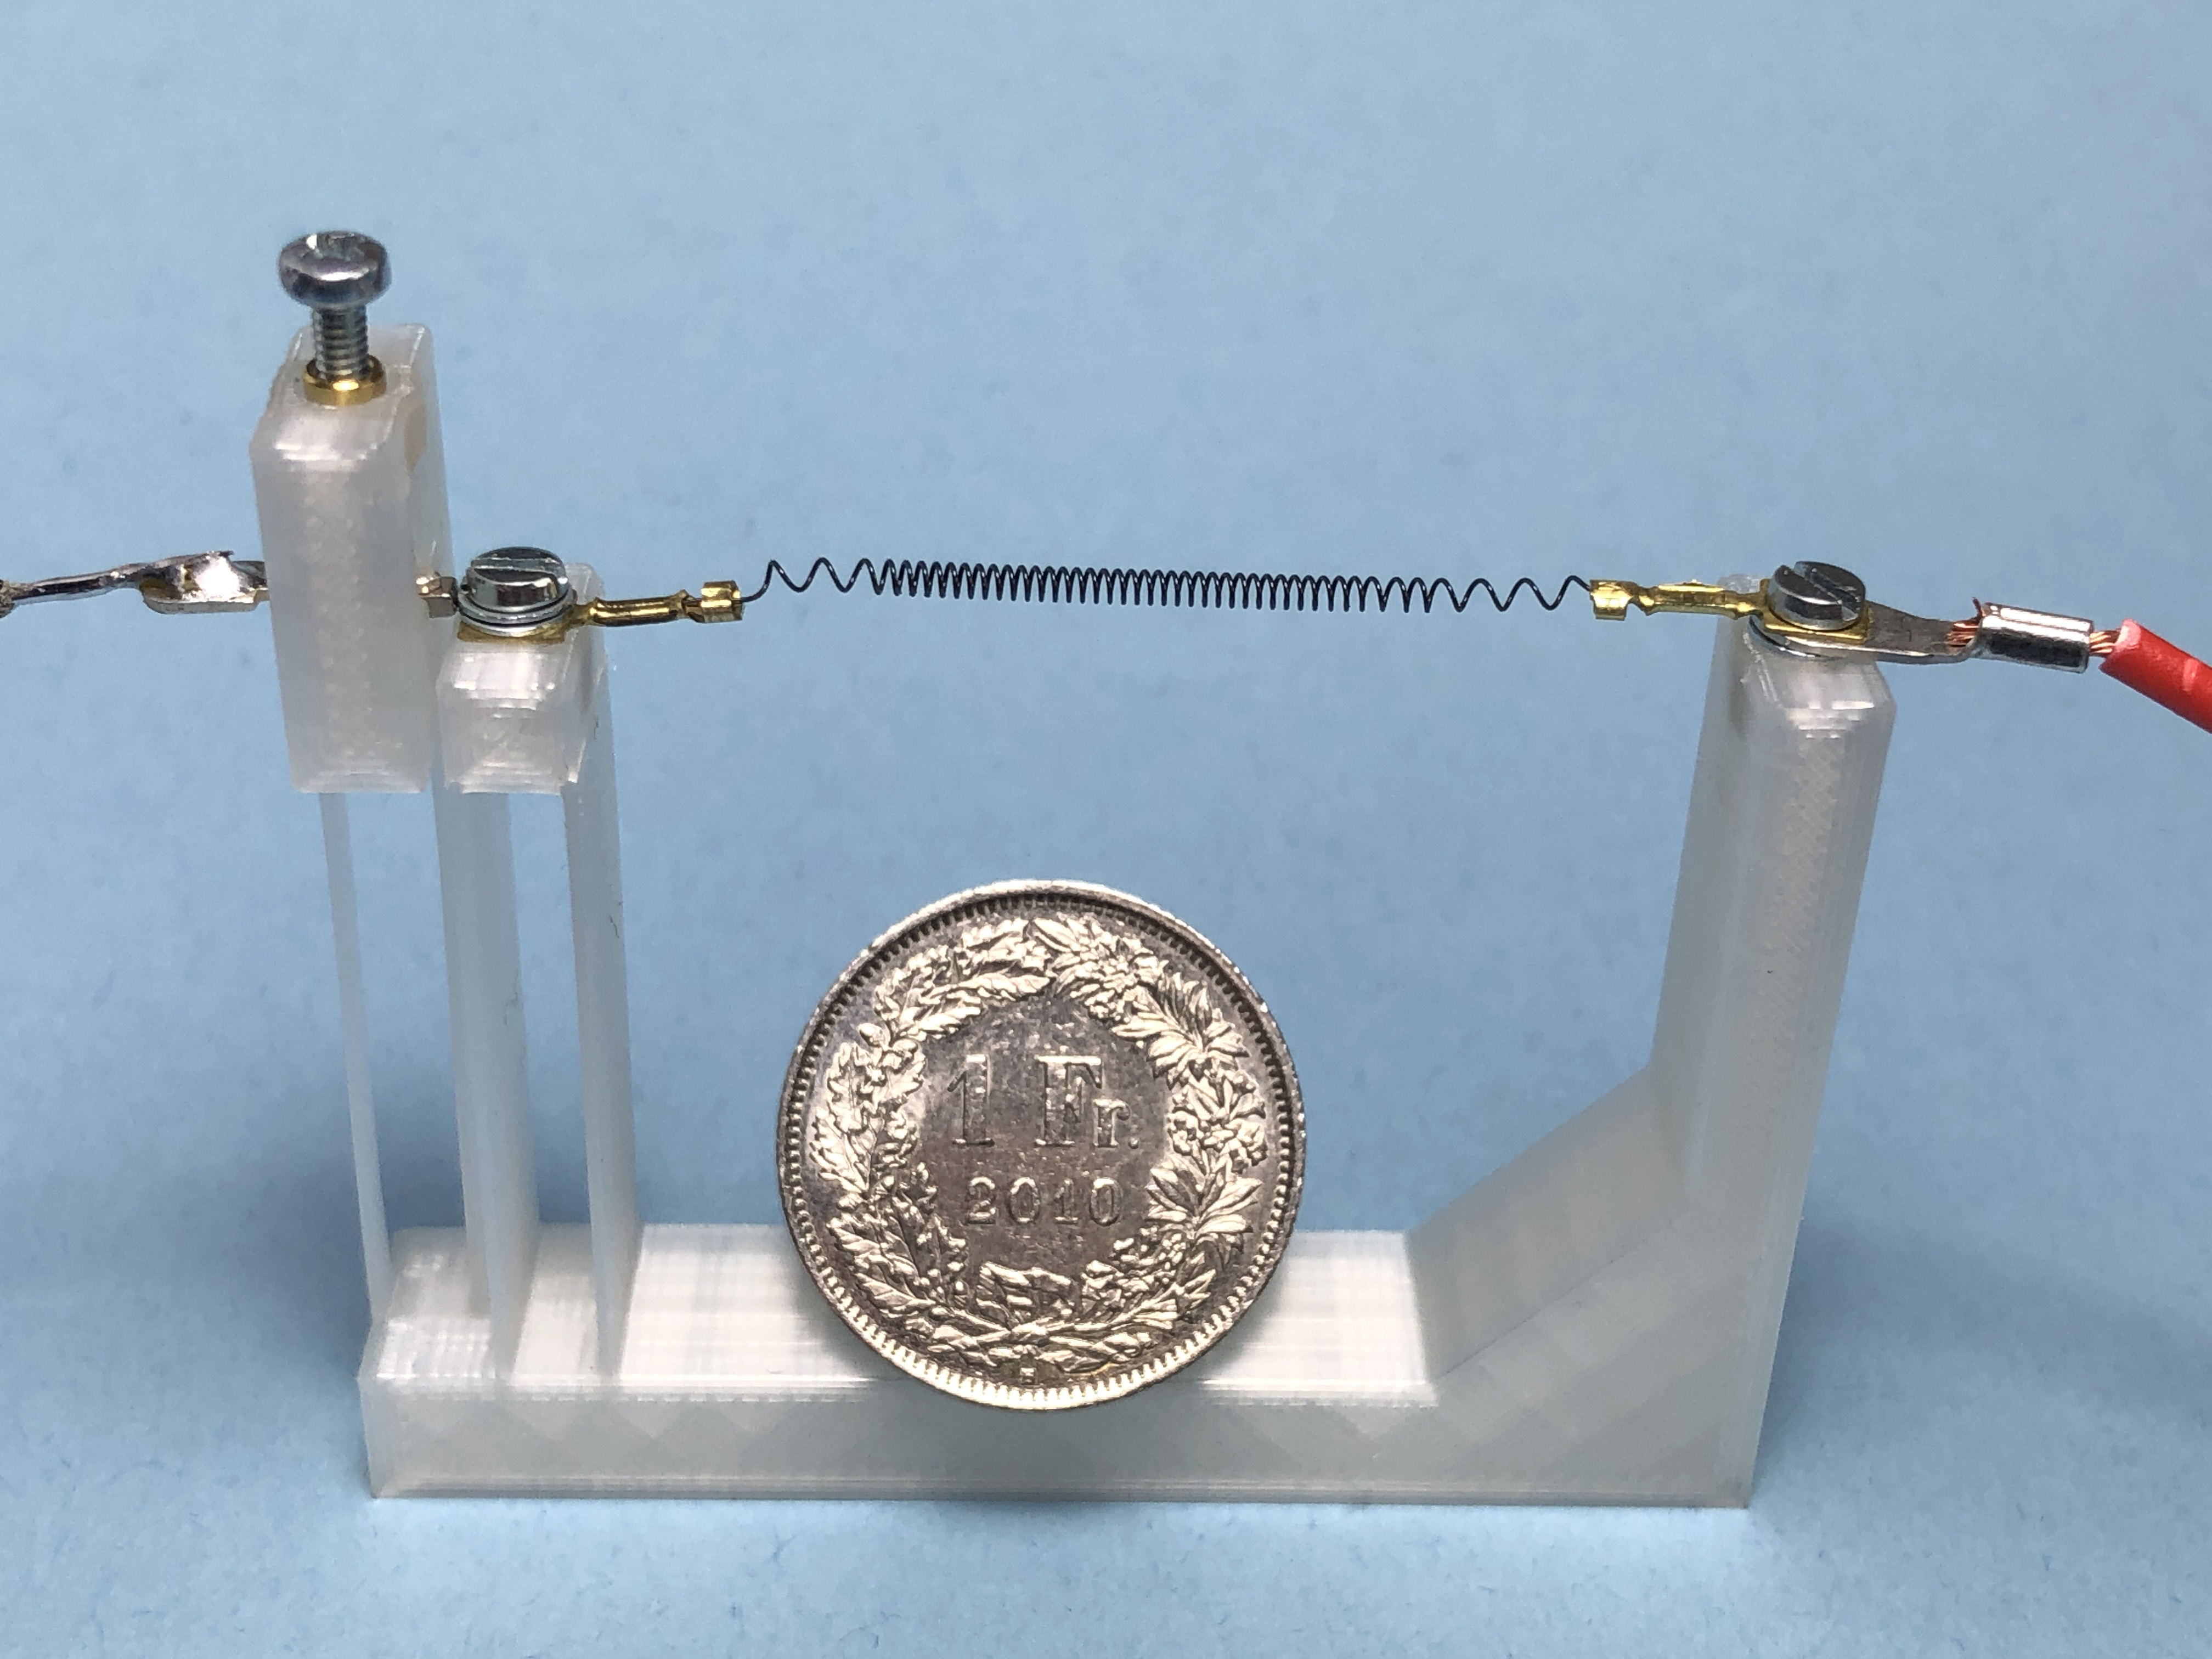
\includegraphics[width=0.75\textwidth]{images/chap6/proto-full.jpg}};
    \end{scope}
  \end{tikzpicture}%
  \caption{The integrated SMA control system implemented using a flexure-based magnetic latch creating an SMA mechanical oscillator.}
  \label{fig:proto-full}
\end{figure}

\begin{figure}[htb!] % t for top of the page, H could be put to impose the position of the float
  \centering
  \begin{annotationimage}{trim={0 0cm 0 20cm},clip, width=0.75\textwidth}{images/chap6/proto-closeup.jpg}
   \draw[annotation right = {SMA Coil at 0.6}] to (0.85,0.48);
   \draw[annotation left = {Magnet at 0.6}] to (0.47,0.5);
   \draw[coordinate label = {Bias Leaf Spring at (0.74,0.1)}];
   \draw[coordinate label = {Leaf Spring at (0.27,0.1)}];
 \end{annotationimage}
  \caption{The close-up structure of the magnetic latch system that acts as the oscillating electrical contact for the SMA coil. Here, the biasing leaf spring also act as a linear stage for the actuator.}
  \label{fig:proto-closeup}
\end{figure}

Here, in this proof-of-concept, the magnetic latch consists of a small magnet, with an attractive force of $150$ g, mounted on a thin leaf spring measuring $500\mu\mathrm{m}\times2.5\mathrm{mm}\times30\mathrm{mm}$. An M2 screw is used to clamp an electrically conductive wire to the magnet and acts as the ground of the electrical circuit. The magnet latches onto another ferromagnetic M2 screw which is mounted to the end-effector of the SMA actuator, as seen in \cref{fig:proto-closeup}. The SMA is supplied by \textit{Dynalloy, Inc} (Irvine, CA) and is a 90\degreeC Flexinol\textsuperscript{\textregistered} coil with wire diameter of 200 $\mu$m and an outer diameter of 1.4 mm. The coil contains around 40 coils and with a solid length of 8 mm. The SMA is mounted on a 3D printed support containing a flexure-based linear stage which supports the free end of the SMA. The linear stage is 3D printed from PLA and consists of 2 parallel leaf springs with dimensions 500 $\mu$m x 10 mm x 30 mm.

This basic concept can be implemented in using different methods. The latch system can be replaced by a bistable mechanism and can then be paired with antagonistic SMA actuators. Here, the control system can be linked to the snap-through of the bistable mechanism where each stable position controls the heating of each SMA element. In this way, the first SMA can be heated till the snap-through of the bistable mechanism which will then change the electrical contact across the antagonistic SMA. This concept has been implemented and validated in \cref{sec:smabb-gripper}.

\subsection{Sizing of the oscillator}
% Sizing strategies (thermal model) + results
% Stroke : rigidity of flexural linear stages; make reference to LDIA paper
As mentioned previously, the thermomechanical behaviour of the SME is exploited to create the mechanical control system. The sizing of the oscillator system is, thus, directly, dependant on the thermal properties of the active element. The rise time or time till the snap-through occurs, depends on the time required to heat the SMA using Joule's heating. This implies that the current supplied across the SMA dictates the rise time of the oscillator. The fall time or time required to re-establish the electrical contact across the SMA depends on the cooling time of the SMA wire or coil. In the case where the SMA is cooled using passive thermal exchange with the surrounding air, the fall time can be controlled by adequately sizing the diameter of the SMA wire or coil. The amplitude of the system, in this case, depends on the latch system and can be sized using the equation \ref{eq:osc-stroke-sizing}. Furthermore, the stroke of the SMA actuator can be sized using the methods presented in \cref{chap:design-methodology} so as to ensure that the actuator is capable of deforming to the levels demanded by the oscillator amplitude. This will ensure that the snap-through of the oscillator occurs before the SMA overheats.

% Cooling time
The fall time of the control system can be calculated using a simple thermal model based on the passive cooling of the SMA wire or coil. Here, the time constant, $\tau_c$, of the system in which the thermal exchange of heat from the surface of the SMA to the surround air is used to cool down the SMA can be expressed as :
\begin{equation}\label{eq:tau}
  \tau_c = \rho cd/(kH)
\end{equation}
where $\rho$ [kg/m$^3$] is the density, $c$ [J/(kgK)] is the specific heat capacity, $d$ is the wire diameter, $k = 4$ is the ratio between the surface area of heat exchange, $A_S$ and the volume of the active element, $V$, and $H$ [W/(m$^2$K)] is the heat transfer coefficient. The thermal model of the wire can be expressed as :
\begin{equation}\label{eq:thermalmodel}
  T(t) = T_R + (T_2-T_R)e^{-t/\tau}
\end{equation}
where $T_R$ is the ambient room temperature and $t$ is time. Thus, the cooling time, $t_c$, based on the temperature gradient between the SMA and the surrounding air, can be expressed as :
\begin{equation}\label{eq:coolingtime}
  t_c = \tau_c\log{\frac{T_2-T_R+\frac{T_2-T_1}{2}}{T_2-T_R-\frac{T_2-T_1}{2}}}
\end{equation}
where the subscripts, 1 and 2, represents the operating points of the actuator as shown in \cref{chap:design-methodology}. The physical properties of the SMA were obtained by consulting the data given by the supplier at \textit{Dynalloy}.

\begin{figure}[htb!] % t for top of the page, H could be put to impose the position of the float
  \centering
  \resizebox{0.8\textwidth}{!}{%% Creator: Matplotlib, PGF backend
%%
%% To include the figure in your LaTeX document, write
%%   \input{<filename>.pgf}
%%
%% Make sure the required packages are loaded in your preamble
%%   \usepackage{pgf}
%%
%% Figures using additional raster images can only be included by \input if
%% they are in the same directory as the main LaTeX file. For loading figures
%% from other directories you can use the `import` package
%%   \usepackage{import}
%% and then include the figures with
%%   \import{<path to file>}{<filename>.pgf}
%%
%% Matplotlib used the following preamble
%%
\begingroup%
\makeatletter%
\begin{pgfpicture}%
\pgfpathrectangle{\pgfpointorigin}{\pgfqpoint{5.757567in}{4.396925in}}%
\pgfusepath{use as bounding box, clip}%
\begin{pgfscope}%
\pgfsetbuttcap%
\pgfsetmiterjoin%
\pgfsetlinewidth{0.000000pt}%
\definecolor{currentstroke}{rgb}{0.000000,0.000000,0.000000}%
\pgfsetstrokecolor{currentstroke}%
\pgfsetstrokeopacity{0.000000}%
\pgfsetdash{}{0pt}%
\pgfpathmoveto{\pgfqpoint{0.000000in}{0.000000in}}%
\pgfpathlineto{\pgfqpoint{5.757567in}{0.000000in}}%
\pgfpathlineto{\pgfqpoint{5.757567in}{4.396925in}}%
\pgfpathlineto{\pgfqpoint{0.000000in}{4.396925in}}%
\pgfpathclose%
\pgfusepath{}%
\end{pgfscope}%
\begin{pgfscope}%
\pgfsetbuttcap%
\pgfsetmiterjoin%
\pgfsetlinewidth{0.000000pt}%
\definecolor{currentstroke}{rgb}{0.000000,0.000000,0.000000}%
\pgfsetstrokecolor{currentstroke}%
\pgfsetstrokeopacity{0.000000}%
\pgfsetdash{}{0pt}%
\pgfpathmoveto{\pgfqpoint{0.697567in}{0.600925in}}%
\pgfpathlineto{\pgfqpoint{5.657567in}{0.600925in}}%
\pgfpathlineto{\pgfqpoint{5.657567in}{4.296925in}}%
\pgfpathlineto{\pgfqpoint{0.697567in}{4.296925in}}%
\pgfpathclose%
\pgfusepath{}%
\end{pgfscope}%
\begin{pgfscope}%
\pgfpathrectangle{\pgfqpoint{0.697567in}{0.600925in}}{\pgfqpoint{4.960000in}{3.696000in}}%
\pgfusepath{clip}%
\pgfsetrectcap%
\pgfsetroundjoin%
\pgfsetlinewidth{0.803000pt}%
\definecolor{currentstroke}{rgb}{0.690196,0.690196,0.690196}%
\pgfsetstrokecolor{currentstroke}%
\pgfsetstrokeopacity{0.200000}%
\pgfsetdash{}{0pt}%
\pgfpathmoveto{\pgfqpoint{0.923021in}{0.600925in}}%
\pgfpathlineto{\pgfqpoint{0.923021in}{4.296925in}}%
\pgfusepath{stroke}%
\end{pgfscope}%
\begin{pgfscope}%
\pgfsetbuttcap%
\pgfsetroundjoin%
\definecolor{currentfill}{rgb}{0.000000,0.000000,0.000000}%
\pgfsetfillcolor{currentfill}%
\pgfsetlinewidth{0.803000pt}%
\definecolor{currentstroke}{rgb}{0.000000,0.000000,0.000000}%
\pgfsetstrokecolor{currentstroke}%
\pgfsetdash{}{0pt}%
\pgfsys@defobject{currentmarker}{\pgfqpoint{0.000000in}{-0.048611in}}{\pgfqpoint{0.000000in}{0.000000in}}{%
\pgfpathmoveto{\pgfqpoint{0.000000in}{0.000000in}}%
\pgfpathlineto{\pgfqpoint{0.000000in}{-0.048611in}}%
\pgfusepath{stroke,fill}%
}%
\begin{pgfscope}%
\pgfsys@transformshift{0.923021in}{0.600925in}%
\pgfsys@useobject{currentmarker}{}%
\end{pgfscope}%
\end{pgfscope}%
\begin{pgfscope}%
\definecolor{textcolor}{rgb}{0.000000,0.000000,0.000000}%
\pgfsetstrokecolor{textcolor}%
\pgfsetfillcolor{textcolor}%
\pgftext[x=0.923021in,y=0.503703in,,top]{\color{textcolor}\rmfamily\fontsize{13.000000}{15.600000}\selectfont \(\displaystyle 0\)}%
\end{pgfscope}%
\begin{pgfscope}%
\pgfpathrectangle{\pgfqpoint{0.697567in}{0.600925in}}{\pgfqpoint{4.960000in}{3.696000in}}%
\pgfusepath{clip}%
\pgfsetrectcap%
\pgfsetroundjoin%
\pgfsetlinewidth{0.803000pt}%
\definecolor{currentstroke}{rgb}{0.690196,0.690196,0.690196}%
\pgfsetstrokecolor{currentstroke}%
\pgfsetstrokeopacity{0.200000}%
\pgfsetdash{}{0pt}%
\pgfpathmoveto{\pgfqpoint{1.672860in}{0.600925in}}%
\pgfpathlineto{\pgfqpoint{1.672860in}{4.296925in}}%
\pgfusepath{stroke}%
\end{pgfscope}%
\begin{pgfscope}%
\pgfsetbuttcap%
\pgfsetroundjoin%
\definecolor{currentfill}{rgb}{0.000000,0.000000,0.000000}%
\pgfsetfillcolor{currentfill}%
\pgfsetlinewidth{0.803000pt}%
\definecolor{currentstroke}{rgb}{0.000000,0.000000,0.000000}%
\pgfsetstrokecolor{currentstroke}%
\pgfsetdash{}{0pt}%
\pgfsys@defobject{currentmarker}{\pgfqpoint{0.000000in}{-0.048611in}}{\pgfqpoint{0.000000in}{0.000000in}}{%
\pgfpathmoveto{\pgfqpoint{0.000000in}{0.000000in}}%
\pgfpathlineto{\pgfqpoint{0.000000in}{-0.048611in}}%
\pgfusepath{stroke,fill}%
}%
\begin{pgfscope}%
\pgfsys@transformshift{1.672860in}{0.600925in}%
\pgfsys@useobject{currentmarker}{}%
\end{pgfscope}%
\end{pgfscope}%
\begin{pgfscope}%
\definecolor{textcolor}{rgb}{0.000000,0.000000,0.000000}%
\pgfsetstrokecolor{textcolor}%
\pgfsetfillcolor{textcolor}%
\pgftext[x=1.672860in,y=0.503703in,,top]{\color{textcolor}\rmfamily\fontsize{13.000000}{15.600000}\selectfont \(\displaystyle 5\)}%
\end{pgfscope}%
\begin{pgfscope}%
\pgfpathrectangle{\pgfqpoint{0.697567in}{0.600925in}}{\pgfqpoint{4.960000in}{3.696000in}}%
\pgfusepath{clip}%
\pgfsetrectcap%
\pgfsetroundjoin%
\pgfsetlinewidth{0.803000pt}%
\definecolor{currentstroke}{rgb}{0.690196,0.690196,0.690196}%
\pgfsetstrokecolor{currentstroke}%
\pgfsetstrokeopacity{0.200000}%
\pgfsetdash{}{0pt}%
\pgfpathmoveto{\pgfqpoint{2.422699in}{0.600925in}}%
\pgfpathlineto{\pgfqpoint{2.422699in}{4.296925in}}%
\pgfusepath{stroke}%
\end{pgfscope}%
\begin{pgfscope}%
\pgfsetbuttcap%
\pgfsetroundjoin%
\definecolor{currentfill}{rgb}{0.000000,0.000000,0.000000}%
\pgfsetfillcolor{currentfill}%
\pgfsetlinewidth{0.803000pt}%
\definecolor{currentstroke}{rgb}{0.000000,0.000000,0.000000}%
\pgfsetstrokecolor{currentstroke}%
\pgfsetdash{}{0pt}%
\pgfsys@defobject{currentmarker}{\pgfqpoint{0.000000in}{-0.048611in}}{\pgfqpoint{0.000000in}{0.000000in}}{%
\pgfpathmoveto{\pgfqpoint{0.000000in}{0.000000in}}%
\pgfpathlineto{\pgfqpoint{0.000000in}{-0.048611in}}%
\pgfusepath{stroke,fill}%
}%
\begin{pgfscope}%
\pgfsys@transformshift{2.422699in}{0.600925in}%
\pgfsys@useobject{currentmarker}{}%
\end{pgfscope}%
\end{pgfscope}%
\begin{pgfscope}%
\definecolor{textcolor}{rgb}{0.000000,0.000000,0.000000}%
\pgfsetstrokecolor{textcolor}%
\pgfsetfillcolor{textcolor}%
\pgftext[x=2.422699in,y=0.503703in,,top]{\color{textcolor}\rmfamily\fontsize{13.000000}{15.600000}\selectfont \(\displaystyle 10\)}%
\end{pgfscope}%
\begin{pgfscope}%
\pgfpathrectangle{\pgfqpoint{0.697567in}{0.600925in}}{\pgfqpoint{4.960000in}{3.696000in}}%
\pgfusepath{clip}%
\pgfsetrectcap%
\pgfsetroundjoin%
\pgfsetlinewidth{0.803000pt}%
\definecolor{currentstroke}{rgb}{0.690196,0.690196,0.690196}%
\pgfsetstrokecolor{currentstroke}%
\pgfsetstrokeopacity{0.200000}%
\pgfsetdash{}{0pt}%
\pgfpathmoveto{\pgfqpoint{3.172538in}{0.600925in}}%
\pgfpathlineto{\pgfqpoint{3.172538in}{4.296925in}}%
\pgfusepath{stroke}%
\end{pgfscope}%
\begin{pgfscope}%
\pgfsetbuttcap%
\pgfsetroundjoin%
\definecolor{currentfill}{rgb}{0.000000,0.000000,0.000000}%
\pgfsetfillcolor{currentfill}%
\pgfsetlinewidth{0.803000pt}%
\definecolor{currentstroke}{rgb}{0.000000,0.000000,0.000000}%
\pgfsetstrokecolor{currentstroke}%
\pgfsetdash{}{0pt}%
\pgfsys@defobject{currentmarker}{\pgfqpoint{0.000000in}{-0.048611in}}{\pgfqpoint{0.000000in}{0.000000in}}{%
\pgfpathmoveto{\pgfqpoint{0.000000in}{0.000000in}}%
\pgfpathlineto{\pgfqpoint{0.000000in}{-0.048611in}}%
\pgfusepath{stroke,fill}%
}%
\begin{pgfscope}%
\pgfsys@transformshift{3.172538in}{0.600925in}%
\pgfsys@useobject{currentmarker}{}%
\end{pgfscope}%
\end{pgfscope}%
\begin{pgfscope}%
\definecolor{textcolor}{rgb}{0.000000,0.000000,0.000000}%
\pgfsetstrokecolor{textcolor}%
\pgfsetfillcolor{textcolor}%
\pgftext[x=3.172538in,y=0.503703in,,top]{\color{textcolor}\rmfamily\fontsize{13.000000}{15.600000}\selectfont \(\displaystyle 15\)}%
\end{pgfscope}%
\begin{pgfscope}%
\pgfpathrectangle{\pgfqpoint{0.697567in}{0.600925in}}{\pgfqpoint{4.960000in}{3.696000in}}%
\pgfusepath{clip}%
\pgfsetrectcap%
\pgfsetroundjoin%
\pgfsetlinewidth{0.803000pt}%
\definecolor{currentstroke}{rgb}{0.690196,0.690196,0.690196}%
\pgfsetstrokecolor{currentstroke}%
\pgfsetstrokeopacity{0.200000}%
\pgfsetdash{}{0pt}%
\pgfpathmoveto{\pgfqpoint{3.922377in}{0.600925in}}%
\pgfpathlineto{\pgfqpoint{3.922377in}{4.296925in}}%
\pgfusepath{stroke}%
\end{pgfscope}%
\begin{pgfscope}%
\pgfsetbuttcap%
\pgfsetroundjoin%
\definecolor{currentfill}{rgb}{0.000000,0.000000,0.000000}%
\pgfsetfillcolor{currentfill}%
\pgfsetlinewidth{0.803000pt}%
\definecolor{currentstroke}{rgb}{0.000000,0.000000,0.000000}%
\pgfsetstrokecolor{currentstroke}%
\pgfsetdash{}{0pt}%
\pgfsys@defobject{currentmarker}{\pgfqpoint{0.000000in}{-0.048611in}}{\pgfqpoint{0.000000in}{0.000000in}}{%
\pgfpathmoveto{\pgfqpoint{0.000000in}{0.000000in}}%
\pgfpathlineto{\pgfqpoint{0.000000in}{-0.048611in}}%
\pgfusepath{stroke,fill}%
}%
\begin{pgfscope}%
\pgfsys@transformshift{3.922377in}{0.600925in}%
\pgfsys@useobject{currentmarker}{}%
\end{pgfscope}%
\end{pgfscope}%
\begin{pgfscope}%
\definecolor{textcolor}{rgb}{0.000000,0.000000,0.000000}%
\pgfsetstrokecolor{textcolor}%
\pgfsetfillcolor{textcolor}%
\pgftext[x=3.922377in,y=0.503703in,,top]{\color{textcolor}\rmfamily\fontsize{13.000000}{15.600000}\selectfont \(\displaystyle 20\)}%
\end{pgfscope}%
\begin{pgfscope}%
\pgfpathrectangle{\pgfqpoint{0.697567in}{0.600925in}}{\pgfqpoint{4.960000in}{3.696000in}}%
\pgfusepath{clip}%
\pgfsetrectcap%
\pgfsetroundjoin%
\pgfsetlinewidth{0.803000pt}%
\definecolor{currentstroke}{rgb}{0.690196,0.690196,0.690196}%
\pgfsetstrokecolor{currentstroke}%
\pgfsetstrokeopacity{0.200000}%
\pgfsetdash{}{0pt}%
\pgfpathmoveto{\pgfqpoint{4.672216in}{0.600925in}}%
\pgfpathlineto{\pgfqpoint{4.672216in}{4.296925in}}%
\pgfusepath{stroke}%
\end{pgfscope}%
\begin{pgfscope}%
\pgfsetbuttcap%
\pgfsetroundjoin%
\definecolor{currentfill}{rgb}{0.000000,0.000000,0.000000}%
\pgfsetfillcolor{currentfill}%
\pgfsetlinewidth{0.803000pt}%
\definecolor{currentstroke}{rgb}{0.000000,0.000000,0.000000}%
\pgfsetstrokecolor{currentstroke}%
\pgfsetdash{}{0pt}%
\pgfsys@defobject{currentmarker}{\pgfqpoint{0.000000in}{-0.048611in}}{\pgfqpoint{0.000000in}{0.000000in}}{%
\pgfpathmoveto{\pgfqpoint{0.000000in}{0.000000in}}%
\pgfpathlineto{\pgfqpoint{0.000000in}{-0.048611in}}%
\pgfusepath{stroke,fill}%
}%
\begin{pgfscope}%
\pgfsys@transformshift{4.672216in}{0.600925in}%
\pgfsys@useobject{currentmarker}{}%
\end{pgfscope}%
\end{pgfscope}%
\begin{pgfscope}%
\definecolor{textcolor}{rgb}{0.000000,0.000000,0.000000}%
\pgfsetstrokecolor{textcolor}%
\pgfsetfillcolor{textcolor}%
\pgftext[x=4.672216in,y=0.503703in,,top]{\color{textcolor}\rmfamily\fontsize{13.000000}{15.600000}\selectfont \(\displaystyle 25\)}%
\end{pgfscope}%
\begin{pgfscope}%
\pgfpathrectangle{\pgfqpoint{0.697567in}{0.600925in}}{\pgfqpoint{4.960000in}{3.696000in}}%
\pgfusepath{clip}%
\pgfsetrectcap%
\pgfsetroundjoin%
\pgfsetlinewidth{0.803000pt}%
\definecolor{currentstroke}{rgb}{0.690196,0.690196,0.690196}%
\pgfsetstrokecolor{currentstroke}%
\pgfsetstrokeopacity{0.200000}%
\pgfsetdash{}{0pt}%
\pgfpathmoveto{\pgfqpoint{5.422055in}{0.600925in}}%
\pgfpathlineto{\pgfqpoint{5.422055in}{4.296925in}}%
\pgfusepath{stroke}%
\end{pgfscope}%
\begin{pgfscope}%
\pgfsetbuttcap%
\pgfsetroundjoin%
\definecolor{currentfill}{rgb}{0.000000,0.000000,0.000000}%
\pgfsetfillcolor{currentfill}%
\pgfsetlinewidth{0.803000pt}%
\definecolor{currentstroke}{rgb}{0.000000,0.000000,0.000000}%
\pgfsetstrokecolor{currentstroke}%
\pgfsetdash{}{0pt}%
\pgfsys@defobject{currentmarker}{\pgfqpoint{0.000000in}{-0.048611in}}{\pgfqpoint{0.000000in}{0.000000in}}{%
\pgfpathmoveto{\pgfqpoint{0.000000in}{0.000000in}}%
\pgfpathlineto{\pgfqpoint{0.000000in}{-0.048611in}}%
\pgfusepath{stroke,fill}%
}%
\begin{pgfscope}%
\pgfsys@transformshift{5.422055in}{0.600925in}%
\pgfsys@useobject{currentmarker}{}%
\end{pgfscope}%
\end{pgfscope}%
\begin{pgfscope}%
\definecolor{textcolor}{rgb}{0.000000,0.000000,0.000000}%
\pgfsetstrokecolor{textcolor}%
\pgfsetfillcolor{textcolor}%
\pgftext[x=5.422055in,y=0.503703in,,top]{\color{textcolor}\rmfamily\fontsize{13.000000}{15.600000}\selectfont \(\displaystyle 30\)}%
\end{pgfscope}%
\begin{pgfscope}%
\definecolor{textcolor}{rgb}{0.000000,0.000000,0.000000}%
\pgfsetstrokecolor{textcolor}%
\pgfsetfillcolor{textcolor}%
\pgftext[x=3.177567in,y=0.300000in,,top]{\color{textcolor}\rmfamily\fontsize{15.000000}{18.000000}\bfseries\selectfont Time [s]}%
\end{pgfscope}%
\begin{pgfscope}%
\pgfpathrectangle{\pgfqpoint{0.697567in}{0.600925in}}{\pgfqpoint{4.960000in}{3.696000in}}%
\pgfusepath{clip}%
\pgfsetrectcap%
\pgfsetroundjoin%
\pgfsetlinewidth{0.803000pt}%
\definecolor{currentstroke}{rgb}{0.690196,0.690196,0.690196}%
\pgfsetstrokecolor{currentstroke}%
\pgfsetstrokeopacity{0.200000}%
\pgfsetdash{}{0pt}%
\pgfpathmoveto{\pgfqpoint{0.697567in}{1.147983in}}%
\pgfpathlineto{\pgfqpoint{5.657567in}{1.147983in}}%
\pgfusepath{stroke}%
\end{pgfscope}%
\begin{pgfscope}%
\pgfsetbuttcap%
\pgfsetroundjoin%
\definecolor{currentfill}{rgb}{0.000000,0.000000,0.000000}%
\pgfsetfillcolor{currentfill}%
\pgfsetlinewidth{0.803000pt}%
\definecolor{currentstroke}{rgb}{0.000000,0.000000,0.000000}%
\pgfsetstrokecolor{currentstroke}%
\pgfsetdash{}{0pt}%
\pgfsys@defobject{currentmarker}{\pgfqpoint{-0.048611in}{0.000000in}}{\pgfqpoint{0.000000in}{0.000000in}}{%
\pgfpathmoveto{\pgfqpoint{0.000000in}{0.000000in}}%
\pgfpathlineto{\pgfqpoint{-0.048611in}{0.000000in}}%
\pgfusepath{stroke,fill}%
}%
\begin{pgfscope}%
\pgfsys@transformshift{0.697567in}{1.147983in}%
\pgfsys@useobject{currentmarker}{}%
\end{pgfscope}%
\end{pgfscope}%
\begin{pgfscope}%
\definecolor{textcolor}{rgb}{0.000000,0.000000,0.000000}%
\pgfsetstrokecolor{textcolor}%
\pgfsetfillcolor{textcolor}%
\pgftext[x=0.437152in,y=1.090113in,left,base]{\color{textcolor}\rmfamily\fontsize{13.000000}{15.600000}\selectfont \(\displaystyle 40\)}%
\end{pgfscope}%
\begin{pgfscope}%
\pgfpathrectangle{\pgfqpoint{0.697567in}{0.600925in}}{\pgfqpoint{4.960000in}{3.696000in}}%
\pgfusepath{clip}%
\pgfsetrectcap%
\pgfsetroundjoin%
\pgfsetlinewidth{0.803000pt}%
\definecolor{currentstroke}{rgb}{0.690196,0.690196,0.690196}%
\pgfsetstrokecolor{currentstroke}%
\pgfsetstrokeopacity{0.200000}%
\pgfsetdash{}{0pt}%
\pgfpathmoveto{\pgfqpoint{0.697567in}{1.884018in}}%
\pgfpathlineto{\pgfqpoint{5.657567in}{1.884018in}}%
\pgfusepath{stroke}%
\end{pgfscope}%
\begin{pgfscope}%
\pgfsetbuttcap%
\pgfsetroundjoin%
\definecolor{currentfill}{rgb}{0.000000,0.000000,0.000000}%
\pgfsetfillcolor{currentfill}%
\pgfsetlinewidth{0.803000pt}%
\definecolor{currentstroke}{rgb}{0.000000,0.000000,0.000000}%
\pgfsetstrokecolor{currentstroke}%
\pgfsetdash{}{0pt}%
\pgfsys@defobject{currentmarker}{\pgfqpoint{-0.048611in}{0.000000in}}{\pgfqpoint{0.000000in}{0.000000in}}{%
\pgfpathmoveto{\pgfqpoint{0.000000in}{0.000000in}}%
\pgfpathlineto{\pgfqpoint{-0.048611in}{0.000000in}}%
\pgfusepath{stroke,fill}%
}%
\begin{pgfscope}%
\pgfsys@transformshift{0.697567in}{1.884018in}%
\pgfsys@useobject{currentmarker}{}%
\end{pgfscope}%
\end{pgfscope}%
\begin{pgfscope}%
\definecolor{textcolor}{rgb}{0.000000,0.000000,0.000000}%
\pgfsetstrokecolor{textcolor}%
\pgfsetfillcolor{textcolor}%
\pgftext[x=0.437152in,y=1.826148in,left,base]{\color{textcolor}\rmfamily\fontsize{13.000000}{15.600000}\selectfont \(\displaystyle 60\)}%
\end{pgfscope}%
\begin{pgfscope}%
\pgfpathrectangle{\pgfqpoint{0.697567in}{0.600925in}}{\pgfqpoint{4.960000in}{3.696000in}}%
\pgfusepath{clip}%
\pgfsetrectcap%
\pgfsetroundjoin%
\pgfsetlinewidth{0.803000pt}%
\definecolor{currentstroke}{rgb}{0.690196,0.690196,0.690196}%
\pgfsetstrokecolor{currentstroke}%
\pgfsetstrokeopacity{0.200000}%
\pgfsetdash{}{0pt}%
\pgfpathmoveto{\pgfqpoint{0.697567in}{2.620053in}}%
\pgfpathlineto{\pgfqpoint{5.657567in}{2.620053in}}%
\pgfusepath{stroke}%
\end{pgfscope}%
\begin{pgfscope}%
\pgfsetbuttcap%
\pgfsetroundjoin%
\definecolor{currentfill}{rgb}{0.000000,0.000000,0.000000}%
\pgfsetfillcolor{currentfill}%
\pgfsetlinewidth{0.803000pt}%
\definecolor{currentstroke}{rgb}{0.000000,0.000000,0.000000}%
\pgfsetstrokecolor{currentstroke}%
\pgfsetdash{}{0pt}%
\pgfsys@defobject{currentmarker}{\pgfqpoint{-0.048611in}{0.000000in}}{\pgfqpoint{0.000000in}{0.000000in}}{%
\pgfpathmoveto{\pgfqpoint{0.000000in}{0.000000in}}%
\pgfpathlineto{\pgfqpoint{-0.048611in}{0.000000in}}%
\pgfusepath{stroke,fill}%
}%
\begin{pgfscope}%
\pgfsys@transformshift{0.697567in}{2.620053in}%
\pgfsys@useobject{currentmarker}{}%
\end{pgfscope}%
\end{pgfscope}%
\begin{pgfscope}%
\definecolor{textcolor}{rgb}{0.000000,0.000000,0.000000}%
\pgfsetstrokecolor{textcolor}%
\pgfsetfillcolor{textcolor}%
\pgftext[x=0.437152in,y=2.562183in,left,base]{\color{textcolor}\rmfamily\fontsize{13.000000}{15.600000}\selectfont \(\displaystyle 80\)}%
\end{pgfscope}%
\begin{pgfscope}%
\pgfpathrectangle{\pgfqpoint{0.697567in}{0.600925in}}{\pgfqpoint{4.960000in}{3.696000in}}%
\pgfusepath{clip}%
\pgfsetrectcap%
\pgfsetroundjoin%
\pgfsetlinewidth{0.803000pt}%
\definecolor{currentstroke}{rgb}{0.690196,0.690196,0.690196}%
\pgfsetstrokecolor{currentstroke}%
\pgfsetstrokeopacity{0.200000}%
\pgfsetdash{}{0pt}%
\pgfpathmoveto{\pgfqpoint{0.697567in}{3.356088in}}%
\pgfpathlineto{\pgfqpoint{5.657567in}{3.356088in}}%
\pgfusepath{stroke}%
\end{pgfscope}%
\begin{pgfscope}%
\pgfsetbuttcap%
\pgfsetroundjoin%
\definecolor{currentfill}{rgb}{0.000000,0.000000,0.000000}%
\pgfsetfillcolor{currentfill}%
\pgfsetlinewidth{0.803000pt}%
\definecolor{currentstroke}{rgb}{0.000000,0.000000,0.000000}%
\pgfsetstrokecolor{currentstroke}%
\pgfsetdash{}{0pt}%
\pgfsys@defobject{currentmarker}{\pgfqpoint{-0.048611in}{0.000000in}}{\pgfqpoint{0.000000in}{0.000000in}}{%
\pgfpathmoveto{\pgfqpoint{0.000000in}{0.000000in}}%
\pgfpathlineto{\pgfqpoint{-0.048611in}{0.000000in}}%
\pgfusepath{stroke,fill}%
}%
\begin{pgfscope}%
\pgfsys@transformshift{0.697567in}{3.356088in}%
\pgfsys@useobject{currentmarker}{}%
\end{pgfscope}%
\end{pgfscope}%
\begin{pgfscope}%
\definecolor{textcolor}{rgb}{0.000000,0.000000,0.000000}%
\pgfsetstrokecolor{textcolor}%
\pgfsetfillcolor{textcolor}%
\pgftext[x=0.355555in,y=3.298218in,left,base]{\color{textcolor}\rmfamily\fontsize{13.000000}{15.600000}\selectfont \(\displaystyle 100\)}%
\end{pgfscope}%
\begin{pgfscope}%
\pgfpathrectangle{\pgfqpoint{0.697567in}{0.600925in}}{\pgfqpoint{4.960000in}{3.696000in}}%
\pgfusepath{clip}%
\pgfsetrectcap%
\pgfsetroundjoin%
\pgfsetlinewidth{0.803000pt}%
\definecolor{currentstroke}{rgb}{0.690196,0.690196,0.690196}%
\pgfsetstrokecolor{currentstroke}%
\pgfsetstrokeopacity{0.200000}%
\pgfsetdash{}{0pt}%
\pgfpathmoveto{\pgfqpoint{0.697567in}{4.092123in}}%
\pgfpathlineto{\pgfqpoint{5.657567in}{4.092123in}}%
\pgfusepath{stroke}%
\end{pgfscope}%
\begin{pgfscope}%
\pgfsetbuttcap%
\pgfsetroundjoin%
\definecolor{currentfill}{rgb}{0.000000,0.000000,0.000000}%
\pgfsetfillcolor{currentfill}%
\pgfsetlinewidth{0.803000pt}%
\definecolor{currentstroke}{rgb}{0.000000,0.000000,0.000000}%
\pgfsetstrokecolor{currentstroke}%
\pgfsetdash{}{0pt}%
\pgfsys@defobject{currentmarker}{\pgfqpoint{-0.048611in}{0.000000in}}{\pgfqpoint{0.000000in}{0.000000in}}{%
\pgfpathmoveto{\pgfqpoint{0.000000in}{0.000000in}}%
\pgfpathlineto{\pgfqpoint{-0.048611in}{0.000000in}}%
\pgfusepath{stroke,fill}%
}%
\begin{pgfscope}%
\pgfsys@transformshift{0.697567in}{4.092123in}%
\pgfsys@useobject{currentmarker}{}%
\end{pgfscope}%
\end{pgfscope}%
\begin{pgfscope}%
\definecolor{textcolor}{rgb}{0.000000,0.000000,0.000000}%
\pgfsetstrokecolor{textcolor}%
\pgfsetfillcolor{textcolor}%
\pgftext[x=0.355555in,y=4.034253in,left,base]{\color{textcolor}\rmfamily\fontsize{13.000000}{15.600000}\selectfont \(\displaystyle 120\)}%
\end{pgfscope}%
\begin{pgfscope}%
\definecolor{textcolor}{rgb}{0.000000,0.000000,0.000000}%
\pgfsetstrokecolor{textcolor}%
\pgfsetfillcolor{textcolor}%
\pgftext[x=0.300000in,y=2.448925in,,bottom,rotate=90.000000]{\color{textcolor}\rmfamily\fontsize{15.000000}{18.000000}\bfseries\selectfont Temperature [°C]}%
\end{pgfscope}%
\begin{pgfscope}%
\pgfpathrectangle{\pgfqpoint{0.697567in}{0.600925in}}{\pgfqpoint{4.960000in}{3.696000in}}%
\pgfusepath{clip}%
\pgfsetrectcap%
\pgfsetroundjoin%
\pgfsetlinewidth{1.505625pt}%
\definecolor{currentstroke}{rgb}{0.411765,0.509804,0.745098}%
\pgfsetstrokecolor{currentstroke}%
\pgfsetdash{}{0pt}%
\pgfpathmoveto{\pgfqpoint{0.923021in}{4.128925in}}%
\pgfpathlineto{\pgfqpoint{0.945606in}{4.055321in}}%
\pgfpathlineto{\pgfqpoint{0.960265in}{3.908114in}}%
\pgfpathlineto{\pgfqpoint{0.972978in}{3.871313in}}%
\pgfpathlineto{\pgfqpoint{0.983149in}{3.871313in}}%
\pgfpathlineto{\pgfqpoint{0.994816in}{3.687304in}}%
\pgfpathlineto{\pgfqpoint{1.005589in}{3.613700in}}%
\pgfpathlineto{\pgfqpoint{1.016059in}{3.466493in}}%
\pgfpathlineto{\pgfqpoint{1.027277in}{3.466493in}}%
\pgfpathlineto{\pgfqpoint{1.038047in}{3.352408in}}%
\pgfpathlineto{\pgfqpoint{1.049794in}{3.308246in}}%
\pgfpathlineto{\pgfqpoint{1.062260in}{3.172079in}}%
\pgfpathlineto{\pgfqpoint{1.069888in}{3.109516in}}%
\pgfpathlineto{\pgfqpoint{1.084546in}{3.109516in}}%
\pgfpathlineto{\pgfqpoint{1.096213in}{2.991751in}}%
\pgfpathlineto{\pgfqpoint{1.107431in}{2.991751in}}%
\pgfpathlineto{\pgfqpoint{1.119097in}{2.862945in}}%
\pgfpathlineto{\pgfqpoint{1.130318in}{2.862945in}}%
\pgfpathlineto{\pgfqpoint{1.141982in}{2.759900in}}%
\pgfpathlineto{\pgfqpoint{1.153350in}{2.712058in}}%
\pgfpathlineto{\pgfqpoint{1.166067in}{2.612693in}}%
\pgfpathlineto{\pgfqpoint{1.174589in}{2.612693in}}%
\pgfpathlineto{\pgfqpoint{1.186554in}{2.542769in}}%
\pgfpathlineto{\pgfqpoint{1.195230in}{2.513328in}}%
\pgfpathlineto{\pgfqpoint{1.206447in}{2.513328in}}%
\pgfpathlineto{\pgfqpoint{1.218114in}{2.425004in}}%
\pgfpathlineto{\pgfqpoint{1.230678in}{2.380842in}}%
\pgfpathlineto{\pgfqpoint{1.238907in}{2.314599in}}%
\pgfpathlineto{\pgfqpoint{1.251319in}{2.314599in}}%
\pgfpathlineto{\pgfqpoint{1.262028in}{2.252036in}}%
\pgfpathlineto{\pgfqpoint{1.273549in}{2.237315in}}%
\pgfpathlineto{\pgfqpoint{1.284613in}{2.237315in}}%
\pgfpathlineto{\pgfqpoint{1.294860in}{2.163711in}}%
\pgfpathlineto{\pgfqpoint{1.305784in}{2.134270in}}%
\pgfpathlineto{\pgfqpoint{1.318193in}{2.068027in}}%
\pgfpathlineto{\pgfqpoint{1.326576in}{2.068027in}}%
\pgfpathlineto{\pgfqpoint{1.337488in}{2.023865in}}%
\pgfpathlineto{\pgfqpoint{1.348258in}{2.005464in}}%
\pgfpathlineto{\pgfqpoint{1.359476in}{2.005464in}}%
\pgfpathlineto{\pgfqpoint{1.370245in}{1.924500in}}%
\pgfpathlineto{\pgfqpoint{1.383410in}{1.924500in}}%
\pgfpathlineto{\pgfqpoint{1.395223in}{1.876658in}}%
\pgfpathlineto{\pgfqpoint{1.408535in}{1.836176in}}%
\pgfpathlineto{\pgfqpoint{1.418407in}{1.810415in}}%
\pgfpathlineto{\pgfqpoint{1.430373in}{1.810415in}}%
\pgfpathlineto{\pgfqpoint{1.441505in}{1.769933in}}%
\pgfpathlineto{\pgfqpoint{1.453171in}{1.751532in}}%
\pgfpathlineto{\pgfqpoint{1.463981in}{1.711050in}}%
\pgfpathlineto{\pgfqpoint{1.476898in}{1.711050in}}%
\pgfpathlineto{\pgfqpoint{1.484636in}{1.677928in}}%
\pgfpathlineto{\pgfqpoint{1.495857in}{1.663208in}}%
\pgfpathlineto{\pgfqpoint{1.506770in}{1.663208in}}%
\pgfpathlineto{\pgfqpoint{1.517919in}{1.630086in}}%
\pgfpathlineto{\pgfqpoint{1.529377in}{1.604325in}}%
\pgfpathlineto{\pgfqpoint{1.541193in}{1.571203in}}%
\pgfpathlineto{\pgfqpoint{1.551443in}{1.571203in}}%
\pgfpathlineto{\pgfqpoint{1.563074in}{1.552802in}}%
\pgfpathlineto{\pgfqpoint{1.573544in}{1.545442in}}%
\pgfpathlineto{\pgfqpoint{1.584167in}{1.545442in}}%
\pgfpathlineto{\pgfqpoint{1.594185in}{1.508640in}}%
\pgfpathlineto{\pgfqpoint{1.605553in}{1.490239in}}%
\pgfpathlineto{\pgfqpoint{1.616472in}{1.464478in}}%
\pgfpathlineto{\pgfqpoint{1.627091in}{1.464478in}}%
\pgfpathlineto{\pgfqpoint{1.638310in}{1.438717in}}%
\pgfpathlineto{\pgfqpoint{1.650424in}{1.442397in}}%
\pgfpathlineto{\pgfqpoint{1.662241in}{1.409275in}}%
\pgfpathlineto{\pgfqpoint{1.673608in}{1.398235in}}%
\pgfpathlineto{\pgfqpoint{1.684078in}{1.398235in}}%
\pgfpathlineto{\pgfqpoint{1.696941in}{1.383514in}}%
\pgfpathlineto{\pgfqpoint{1.705168in}{1.383514in}}%
\pgfpathlineto{\pgfqpoint{1.716611in}{1.368794in}}%
\pgfpathlineto{\pgfqpoint{1.729026in}{1.354073in}}%
\pgfpathlineto{\pgfqpoint{1.737252in}{1.331992in}}%
\pgfpathlineto{\pgfqpoint{1.749451in}{1.328312in}}%
\pgfpathlineto{\pgfqpoint{1.757227in}{1.328312in}}%
\pgfpathlineto{\pgfqpoint{1.769941in}{1.302550in}}%
\pgfpathlineto{\pgfqpoint{1.781757in}{1.302550in}}%
\pgfpathlineto{\pgfqpoint{1.793574in}{1.280469in}}%
\pgfpathlineto{\pgfqpoint{1.802100in}{1.280469in}}%
\pgfpathlineto{\pgfqpoint{1.813467in}{1.262068in}}%
\pgfpathlineto{\pgfqpoint{1.824236in}{1.254708in}}%
\pgfpathlineto{\pgfqpoint{1.834258in}{1.254708in}}%
\pgfpathlineto{\pgfqpoint{1.845475in}{1.236307in}}%
\pgfpathlineto{\pgfqpoint{1.856544in}{1.236307in}}%
\pgfpathlineto{\pgfqpoint{1.868061in}{1.203186in}}%
\pgfpathlineto{\pgfqpoint{1.881373in}{1.203186in}}%
\pgfpathlineto{\pgfqpoint{1.893339in}{1.195825in}}%
\pgfpathlineto{\pgfqpoint{1.906651in}{1.188465in}}%
\pgfpathlineto{\pgfqpoint{1.918019in}{1.170064in}}%
\pgfpathlineto{\pgfqpoint{1.928189in}{1.170064in}}%
\pgfpathlineto{\pgfqpoint{1.938958in}{1.162704in}}%
\pgfpathlineto{\pgfqpoint{1.950924in}{1.162704in}}%
\pgfpathlineto{\pgfqpoint{1.961795in}{1.136943in}}%
\pgfpathlineto{\pgfqpoint{1.974062in}{1.129582in}}%
\pgfpathlineto{\pgfqpoint{1.984529in}{1.129582in}}%
\pgfpathlineto{\pgfqpoint{1.995897in}{1.136943in}}%
\pgfpathlineto{\pgfqpoint{2.008358in}{1.125902in}}%
\pgfpathlineto{\pgfqpoint{2.022345in}{1.114861in}}%
\pgfpathlineto{\pgfqpoint{2.032444in}{1.114861in}}%
\pgfpathlineto{\pgfqpoint{2.043209in}{1.107501in}}%
\pgfpathlineto{\pgfqpoint{2.055623in}{1.103821in}}%
\pgfpathlineto{\pgfqpoint{2.065944in}{1.111181in}}%
\pgfpathlineto{\pgfqpoint{2.077614in}{1.111181in}}%
\pgfpathlineto{\pgfqpoint{2.086140in}{1.085420in}}%
\pgfpathlineto{\pgfqpoint{2.097204in}{1.096461in}}%
\pgfpathlineto{\pgfqpoint{2.108123in}{1.096461in}}%
\pgfpathlineto{\pgfqpoint{2.120238in}{1.074380in}}%
\pgfpathlineto{\pgfqpoint{2.132653in}{1.074380in}}%
\pgfpathlineto{\pgfqpoint{2.144469in}{1.067019in}}%
\pgfpathlineto{\pgfqpoint{2.156290in}{1.067019in}}%
\pgfpathlineto{\pgfqpoint{2.166832in}{1.055979in}}%
\pgfpathlineto{\pgfqpoint{2.179546in}{1.055979in}}%
\pgfpathlineto{\pgfqpoint{2.191813in}{1.044938in}}%
\pgfpathlineto{\pgfqpoint{2.204174in}{1.041258in}}%
\pgfpathlineto{\pgfqpoint{2.215392in}{1.030217in}}%
\pgfpathlineto{\pgfqpoint{2.226101in}{1.030217in}}%
\pgfpathlineto{\pgfqpoint{2.238605in}{1.015497in}}%
\pgfpathlineto{\pgfqpoint{2.250270in}{1.008136in}}%
\pgfpathlineto{\pgfqpoint{2.261338in}{1.004456in}}%
\pgfpathlineto{\pgfqpoint{2.273530in}{0.997096in}}%
\pgfpathlineto{\pgfqpoint{2.285047in}{0.997096in}}%
\pgfpathlineto{\pgfqpoint{2.297162in}{1.000776in}}%
\pgfpathlineto{\pgfqpoint{2.308829in}{0.993416in}}%
\pgfpathlineto{\pgfqpoint{2.332910in}{0.993416in}}%
\pgfpathlineto{\pgfqpoint{2.355495in}{0.978695in}}%
\pgfpathlineto{\pgfqpoint{2.365519in}{0.967654in}}%
\pgfpathlineto{\pgfqpoint{2.389149in}{0.967654in}}%
\pgfpathlineto{\pgfqpoint{2.400670in}{0.963974in}}%
\pgfpathlineto{\pgfqpoint{2.413829in}{0.956614in}}%
\pgfpathlineto{\pgfqpoint{2.447550in}{0.956614in}}%
\pgfpathlineto{\pgfqpoint{2.461759in}{0.945573in}}%
\pgfpathlineto{\pgfqpoint{2.473575in}{0.941893in}}%
\pgfpathlineto{\pgfqpoint{2.484195in}{0.941893in}}%
\pgfpathlineto{\pgfqpoint{2.495113in}{0.934533in}}%
\pgfpathlineto{\pgfqpoint{2.527720in}{0.934533in}}%
\pgfpathlineto{\pgfqpoint{2.539835in}{0.938213in}}%
\pgfpathlineto{\pgfqpoint{2.550605in}{0.934533in}}%
\pgfpathlineto{\pgfqpoint{2.576182in}{0.919812in}}%
\pgfpathlineto{\pgfqpoint{2.585455in}{0.919812in}}%
\pgfpathlineto{\pgfqpoint{2.596823in}{0.916132in}}%
\pgfpathlineto{\pgfqpoint{2.609536in}{0.912452in}}%
\pgfpathlineto{\pgfqpoint{2.632421in}{0.912452in}}%
\pgfpathlineto{\pgfqpoint{2.645733in}{0.897731in}}%
\pgfpathlineto{\pgfqpoint{2.658297in}{0.897731in}}%
\pgfpathlineto{\pgfqpoint{2.666075in}{0.901411in}}%
\pgfpathlineto{\pgfqpoint{2.677373in}{0.901411in}}%
\pgfpathlineto{\pgfqpoint{2.689488in}{0.894051in}}%
\pgfpathlineto{\pgfqpoint{2.733427in}{0.894051in}}%
\pgfpathlineto{\pgfqpoint{2.744495in}{0.897731in}}%
\pgfpathlineto{\pgfqpoint{2.852337in}{0.897731in}}%
\pgfpathlineto{\pgfqpoint{2.862808in}{0.875650in}}%
\pgfpathlineto{\pgfqpoint{2.875671in}{0.860929in}}%
\pgfpathlineto{\pgfqpoint{2.888086in}{0.860929in}}%
\pgfpathlineto{\pgfqpoint{2.902445in}{0.857249in}}%
\pgfpathlineto{\pgfqpoint{2.915241in}{0.857249in}}%
\pgfpathlineto{\pgfqpoint{2.927505in}{0.864610in}}%
\pgfpathlineto{\pgfqpoint{2.938949in}{0.849889in}}%
\pgfpathlineto{\pgfqpoint{2.950691in}{0.853569in}}%
\pgfpathlineto{\pgfqpoint{2.972007in}{0.853569in}}%
\pgfpathlineto{\pgfqpoint{2.983374in}{0.860929in}}%
\pgfpathlineto{\pgfqpoint{2.996686in}{0.849889in}}%
\pgfpathlineto{\pgfqpoint{3.008353in}{0.849889in}}%
\pgfpathlineto{\pgfqpoint{3.024956in}{0.838848in}}%
\pgfpathlineto{\pgfqpoint{3.058609in}{0.838848in}}%
\pgfpathlineto{\pgfqpoint{3.070726in}{0.849889in}}%
\pgfpathlineto{\pgfqpoint{3.078801in}{0.849889in}}%
\pgfpathlineto{\pgfqpoint{3.091515in}{0.846209in}}%
\pgfpathlineto{\pgfqpoint{3.102596in}{0.838848in}}%
\pgfpathlineto{\pgfqpoint{3.113518in}{0.838848in}}%
\pgfpathlineto{\pgfqpoint{3.124771in}{0.846209in}}%
\pgfpathlineto{\pgfqpoint{3.135391in}{0.827808in}}%
\pgfpathlineto{\pgfqpoint{3.158814in}{0.827808in}}%
\pgfpathlineto{\pgfqpoint{3.170863in}{0.824128in}}%
\pgfpathlineto{\pgfqpoint{3.184923in}{0.824128in}}%
\pgfpathlineto{\pgfqpoint{3.196589in}{0.827808in}}%
\pgfpathlineto{\pgfqpoint{3.208835in}{0.827808in}}%
\pgfpathlineto{\pgfqpoint{3.220648in}{0.831488in}}%
\pgfpathlineto{\pgfqpoint{3.231866in}{0.831488in}}%
\pgfpathlineto{\pgfqpoint{3.257293in}{0.816767in}}%
\pgfpathlineto{\pgfqpoint{3.269259in}{0.813087in}}%
\pgfpathlineto{\pgfqpoint{3.280028in}{0.813087in}}%
\pgfpathlineto{\pgfqpoint{3.291695in}{0.824128in}}%
\pgfpathlineto{\pgfqpoint{3.304413in}{0.824128in}}%
\pgfpathlineto{\pgfqpoint{3.315626in}{0.813087in}}%
\pgfpathlineto{\pgfqpoint{3.326844in}{0.813087in}}%
\pgfpathlineto{\pgfqpoint{3.339109in}{0.816767in}}%
\pgfpathlineto{\pgfqpoint{3.365284in}{0.816767in}}%
\pgfpathlineto{\pgfqpoint{3.376026in}{0.813087in}}%
\pgfpathlineto{\pgfqpoint{3.387095in}{0.802047in}}%
\pgfpathlineto{\pgfqpoint{3.397266in}{0.805727in}}%
\pgfpathlineto{\pgfqpoint{3.420150in}{0.805727in}}%
\pgfpathlineto{\pgfqpoint{3.432940in}{0.802047in}}%
\pgfpathlineto{\pgfqpoint{3.479982in}{0.802047in}}%
\pgfpathlineto{\pgfqpoint{3.490452in}{0.805727in}}%
\pgfpathlineto{\pgfqpoint{3.501221in}{0.805727in}}%
\pgfpathlineto{\pgfqpoint{3.512439in}{0.798366in}}%
\pgfpathlineto{\pgfqpoint{3.533229in}{0.798366in}}%
\pgfpathlineto{\pgfqpoint{3.544896in}{0.791006in}}%
\pgfpathlineto{\pgfqpoint{3.557460in}{0.791006in}}%
\pgfpathlineto{\pgfqpoint{3.568678in}{0.802047in}}%
\pgfpathlineto{\pgfqpoint{3.580195in}{0.802047in}}%
\pgfpathlineto{\pgfqpoint{3.589169in}{0.787326in}}%
\pgfpathlineto{\pgfqpoint{3.600687in}{0.791006in}}%
\pgfpathlineto{\pgfqpoint{3.612401in}{0.791006in}}%
\pgfpathlineto{\pgfqpoint{3.623616in}{0.798366in}}%
\pgfpathlineto{\pgfqpoint{3.635232in}{0.798366in}}%
\pgfpathlineto{\pgfqpoint{3.647199in}{0.787326in}}%
\pgfpathlineto{\pgfqpoint{3.657910in}{0.791006in}}%
\pgfpathlineto{\pgfqpoint{3.669875in}{0.798366in}}%
\pgfpathlineto{\pgfqpoint{3.680863in}{0.798366in}}%
\pgfpathlineto{\pgfqpoint{3.693277in}{0.783646in}}%
\pgfpathlineto{\pgfqpoint{3.736657in}{0.783646in}}%
\pgfpathlineto{\pgfqpoint{3.747423in}{0.791006in}}%
\pgfpathlineto{\pgfqpoint{3.759239in}{0.791006in}}%
\pgfpathlineto{\pgfqpoint{3.771205in}{0.783646in}}%
\pgfpathlineto{\pgfqpoint{3.784068in}{0.783646in}}%
\pgfpathlineto{\pgfqpoint{3.791995in}{0.787326in}}%
\pgfpathlineto{\pgfqpoint{3.802764in}{0.787326in}}%
\pgfpathlineto{\pgfqpoint{3.813833in}{0.772605in}}%
\pgfpathlineto{\pgfqpoint{3.825948in}{0.783646in}}%
\pgfpathlineto{\pgfqpoint{3.836570in}{0.772605in}}%
\pgfpathlineto{\pgfqpoint{3.861697in}{0.772605in}}%
\pgfpathlineto{\pgfqpoint{3.873779in}{0.783646in}}%
\pgfpathlineto{\pgfqpoint{3.937796in}{0.783646in}}%
\pgfpathlineto{\pgfqpoint{3.948715in}{0.791006in}}%
\pgfpathlineto{\pgfqpoint{3.959933in}{0.779966in}}%
\pgfpathlineto{\pgfqpoint{3.971450in}{0.783646in}}%
\pgfpathlineto{\pgfqpoint{3.982518in}{0.783646in}}%
\pgfpathlineto{\pgfqpoint{3.994051in}{0.779966in}}%
\pgfpathlineto{\pgfqpoint{4.003907in}{0.779966in}}%
\pgfpathlineto{\pgfqpoint{4.015574in}{0.783646in}}%
\pgfpathlineto{\pgfqpoint{4.027167in}{0.783646in}}%
\pgfpathlineto{\pgfqpoint{4.038128in}{0.772605in}}%
\pgfpathlineto{\pgfqpoint{4.084273in}{0.772605in}}%
\pgfpathlineto{\pgfqpoint{4.094444in}{0.779966in}}%
\pgfpathlineto{\pgfqpoint{4.106559in}{0.779966in}}%
\pgfpathlineto{\pgfqpoint{4.118926in}{0.783646in}}%
\pgfpathlineto{\pgfqpoint{4.130258in}{0.783646in}}%
\pgfpathlineto{\pgfqpoint{4.142221in}{0.776285in}}%
\pgfpathlineto{\pgfqpoint{4.154486in}{0.772605in}}%
\pgfpathlineto{\pgfqpoint{4.166082in}{0.779966in}}%
\pgfpathlineto{\pgfqpoint{4.185976in}{0.779966in}}%
\pgfpathlineto{\pgfqpoint{4.197048in}{0.776285in}}%
\pgfpathlineto{\pgfqpoint{4.207514in}{0.776285in}}%
\pgfpathlineto{\pgfqpoint{4.217834in}{0.772605in}}%
\pgfpathlineto{\pgfqpoint{4.229950in}{0.772605in}}%
\pgfpathlineto{\pgfqpoint{4.242065in}{0.779966in}}%
\pgfpathlineto{\pgfqpoint{4.253582in}{0.779966in}}%
\pgfpathlineto{\pgfqpoint{4.264501in}{0.768925in}}%
\pgfpathlineto{\pgfqpoint{4.273326in}{0.779966in}}%
\pgfpathlineto{\pgfqpoint{4.284095in}{0.779966in}}%
\pgfpathlineto{\pgfqpoint{4.295462in}{0.772605in}}%
\pgfpathlineto{\pgfqpoint{4.305788in}{0.772605in}}%
\pgfpathlineto{\pgfqpoint{4.316417in}{0.776285in}}%
\pgfpathlineto{\pgfqpoint{4.337472in}{0.776285in}}%
\pgfpathlineto{\pgfqpoint{4.347343in}{0.783646in}}%
\pgfpathlineto{\pgfqpoint{4.358561in}{0.783646in}}%
\pgfpathlineto{\pgfqpoint{4.369772in}{0.776285in}}%
\pgfpathlineto{\pgfqpoint{4.409266in}{0.776285in}}%
\pgfpathlineto{\pgfqpoint{4.421232in}{0.779966in}}%
\pgfpathlineto{\pgfqpoint{4.433048in}{0.779966in}}%
\pgfpathlineto{\pgfqpoint{4.444265in}{0.768925in}}%
\pgfpathlineto{\pgfqpoint{4.465355in}{0.776285in}}%
\pgfpathlineto{\pgfqpoint{4.487342in}{0.776285in}}%
\pgfpathlineto{\pgfqpoint{4.499158in}{0.772605in}}%
\pgfpathlineto{\pgfqpoint{4.510825in}{0.776285in}}%
\pgfpathlineto{\pgfqpoint{4.522492in}{0.772605in}}%
\pgfpathlineto{\pgfqpoint{4.578581in}{0.772605in}}%
\pgfpathlineto{\pgfqpoint{4.589800in}{0.776285in}}%
\pgfpathlineto{\pgfqpoint{4.655654in}{0.776285in}}%
\pgfpathlineto{\pgfqpoint{4.665825in}{0.772605in}}%
\pgfpathlineto{\pgfqpoint{4.677791in}{0.768925in}}%
\pgfpathlineto{\pgfqpoint{4.689607in}{0.783646in}}%
\pgfpathlineto{\pgfqpoint{4.700226in}{0.783646in}}%
\pgfpathlineto{\pgfqpoint{4.711445in}{0.779966in}}%
\pgfpathlineto{\pgfqpoint{4.723261in}{0.783646in}}%
\pgfpathlineto{\pgfqpoint{4.734339in}{0.783646in}}%
\pgfpathlineto{\pgfqpoint{4.745846in}{0.772605in}}%
\pgfpathlineto{\pgfqpoint{4.757363in}{0.772605in}}%
\pgfpathlineto{\pgfqpoint{4.769478in}{0.783646in}}%
\pgfpathlineto{\pgfqpoint{4.780248in}{0.783646in}}%
\pgfpathlineto{\pgfqpoint{4.792513in}{0.787326in}}%
\pgfpathlineto{\pgfqpoint{4.801940in}{0.787326in}}%
\pgfpathlineto{\pgfqpoint{4.813459in}{0.772605in}}%
\pgfpathlineto{\pgfqpoint{4.825423in}{0.776285in}}%
\pgfpathlineto{\pgfqpoint{4.856522in}{0.776285in}}%
\pgfpathlineto{\pgfqpoint{4.867966in}{0.779966in}}%
\pgfpathlineto{\pgfqpoint{4.880381in}{0.779966in}}%
\pgfpathlineto{\pgfqpoint{4.891299in}{0.783646in}}%
\pgfpathlineto{\pgfqpoint{4.903116in}{0.772605in}}%
\pgfpathlineto{\pgfqpoint{4.913737in}{0.779966in}}%
\pgfpathlineto{\pgfqpoint{4.925551in}{0.779966in}}%
\pgfpathlineto{\pgfqpoint{4.936919in}{0.772605in}}%
\pgfpathlineto{\pgfqpoint{4.948137in}{0.779966in}}%
\pgfpathlineto{\pgfqpoint{4.962346in}{0.776285in}}%
\pgfpathlineto{\pgfqpoint{4.986727in}{0.776285in}}%
\pgfpathlineto{\pgfqpoint{4.998244in}{0.772605in}}%
\pgfpathlineto{\pgfqpoint{5.009687in}{0.772605in}}%
\pgfpathlineto{\pgfqpoint{5.020905in}{0.783646in}}%
\pgfpathlineto{\pgfqpoint{5.032012in}{0.783646in}}%
\pgfpathlineto{\pgfqpoint{5.044277in}{0.776285in}}%
\pgfpathlineto{\pgfqpoint{5.056042in}{0.772605in}}%
\pgfpathlineto{\pgfqpoint{5.068156in}{0.776285in}}%
\pgfpathlineto{\pgfqpoint{5.079673in}{0.776285in}}%
\pgfpathlineto{\pgfqpoint{5.090742in}{0.779966in}}%
\pgfpathlineto{\pgfqpoint{5.102192in}{0.779966in}}%
\pgfpathlineto{\pgfqpoint{5.115286in}{0.776285in}}%
\pgfpathlineto{\pgfqpoint{5.159854in}{0.776285in}}%
\pgfpathlineto{\pgfqpoint{5.172120in}{0.787326in}}%
\pgfpathlineto{\pgfqpoint{5.180345in}{0.787326in}}%
\pgfpathlineto{\pgfqpoint{5.192012in}{0.779966in}}%
\pgfpathlineto{\pgfqpoint{5.205474in}{0.776285in}}%
\pgfpathlineto{\pgfqpoint{5.216841in}{0.779966in}}%
\pgfpathlineto{\pgfqpoint{5.240477in}{0.779966in}}%
\pgfpathlineto{\pgfqpoint{5.254234in}{0.772605in}}%
\pgfpathlineto{\pgfqpoint{5.267622in}{0.776285in}}%
\pgfpathlineto{\pgfqpoint{5.280037in}{0.772605in}}%
\pgfpathlineto{\pgfqpoint{5.291812in}{0.776285in}}%
\pgfpathlineto{\pgfqpoint{5.303479in}{0.776285in}}%
\pgfpathlineto{\pgfqpoint{5.314697in}{0.772605in}}%
\pgfpathlineto{\pgfqpoint{5.327114in}{0.779966in}}%
\pgfpathlineto{\pgfqpoint{5.351791in}{0.772605in}}%
\pgfpathlineto{\pgfqpoint{5.364953in}{0.783646in}}%
\pgfpathlineto{\pgfqpoint{5.374675in}{0.783646in}}%
\pgfpathlineto{\pgfqpoint{5.411320in}{0.772605in}}%
\pgfpathlineto{\pgfqpoint{5.432112in}{0.772605in}}%
\pgfpathlineto{\pgfqpoint{5.432112in}{0.772605in}}%
\pgfusepath{stroke}%
\end{pgfscope}%
\begin{pgfscope}%
\pgfpathrectangle{\pgfqpoint{0.697567in}{0.600925in}}{\pgfqpoint{4.960000in}{3.696000in}}%
\pgfusepath{clip}%
\pgfsetbuttcap%
\pgfsetroundjoin%
\pgfsetlinewidth{1.505625pt}%
\definecolor{currentstroke}{rgb}{0.286275,0.666667,0.435294}%
\pgfsetstrokecolor{currentstroke}%
\pgfsetdash{{5.550000pt}{2.400000pt}}{0.000000pt}%
\pgfpathmoveto{\pgfqpoint{0.923021in}{4.128925in}}%
\pgfpathlineto{\pgfqpoint{0.960265in}{4.033286in}}%
\pgfpathlineto{\pgfqpoint{0.994816in}{3.946996in}}%
\pgfpathlineto{\pgfqpoint{1.027277in}{3.868003in}}%
\pgfpathlineto{\pgfqpoint{1.062260in}{3.785074in}}%
\pgfpathlineto{\pgfqpoint{1.096213in}{3.706708in}}%
\pgfpathlineto{\pgfqpoint{1.130318in}{3.630039in}}%
\pgfpathlineto{\pgfqpoint{1.166067in}{3.551823in}}%
\pgfpathlineto{\pgfqpoint{1.195230in}{3.489603in}}%
\pgfpathlineto{\pgfqpoint{1.230678in}{3.415843in}}%
\pgfpathlineto{\pgfqpoint{1.262028in}{3.352279in}}%
\pgfpathlineto{\pgfqpoint{1.294860in}{3.287345in}}%
\pgfpathlineto{\pgfqpoint{1.326576in}{3.226170in}}%
\pgfpathlineto{\pgfqpoint{1.359476in}{3.164280in}}%
\pgfpathlineto{\pgfqpoint{1.395223in}{3.098799in}}%
\pgfpathlineto{\pgfqpoint{1.430373in}{3.036159in}}%
\pgfpathlineto{\pgfqpoint{1.463981in}{2.977841in}}%
\pgfpathlineto{\pgfqpoint{1.495857in}{2.923917in}}%
\pgfpathlineto{\pgfqpoint{1.529377in}{2.868630in}}%
\pgfpathlineto{\pgfqpoint{1.563074in}{2.814481in}}%
\pgfpathlineto{\pgfqpoint{1.594185in}{2.765727in}}%
\pgfpathlineto{\pgfqpoint{1.627091in}{2.715426in}}%
\pgfpathlineto{\pgfqpoint{1.662241in}{2.663093in}}%
\pgfpathlineto{\pgfqpoint{1.696941in}{2.612809in}}%
\pgfpathlineto{\pgfqpoint{1.729026in}{2.567504in}}%
\pgfpathlineto{\pgfqpoint{1.757227in}{2.528603in}}%
\pgfpathlineto{\pgfqpoint{1.793574in}{2.479704in}}%
\pgfpathlineto{\pgfqpoint{1.824236in}{2.439511in}}%
\pgfpathlineto{\pgfqpoint{1.856544in}{2.398183in}}%
\pgfpathlineto{\pgfqpoint{1.893339in}{2.352358in}}%
\pgfpathlineto{\pgfqpoint{1.928189in}{2.310144in}}%
\pgfpathlineto{\pgfqpoint{1.961795in}{2.270504in}}%
\pgfpathlineto{\pgfqpoint{1.995897in}{2.231320in}}%
\pgfpathlineto{\pgfqpoint{2.032444in}{2.190462in}}%
\pgfpathlineto{\pgfqpoint{2.065944in}{2.154014in}}%
\pgfpathlineto{\pgfqpoint{2.108123in}{2.109448in}}%
\pgfpathlineto{\pgfqpoint{2.144469in}{2.072198in}}%
\pgfpathlineto{\pgfqpoint{2.179546in}{2.037230in}}%
\pgfpathlineto{\pgfqpoint{2.215392in}{2.002465in}}%
\pgfpathlineto{\pgfqpoint{2.250270in}{1.969553in}}%
\pgfpathlineto{\pgfqpoint{2.285047in}{1.937611in}}%
\pgfpathlineto{\pgfqpoint{2.321542in}{1.905004in}}%
\pgfpathlineto{\pgfqpoint{2.365519in}{1.866920in}}%
\pgfpathlineto{\pgfqpoint{2.400670in}{1.837398in}}%
\pgfpathlineto{\pgfqpoint{2.435741in}{1.808735in}}%
\pgfpathlineto{\pgfqpoint{2.473575in}{1.778675in}}%
\pgfpathlineto{\pgfqpoint{2.517250in}{1.745054in}}%
\pgfpathlineto{\pgfqpoint{2.550605in}{1.720133in}}%
\pgfpathlineto{\pgfqpoint{2.596823in}{1.686649in}}%
\pgfpathlineto{\pgfqpoint{2.632421in}{1.661665in}}%
\pgfpathlineto{\pgfqpoint{2.677373in}{1.631086in}}%
\pgfpathlineto{\pgfqpoint{2.721760in}{1.601918in}}%
\pgfpathlineto{\pgfqpoint{2.768427in}{1.572316in}}%
\pgfpathlineto{\pgfqpoint{2.814346in}{1.544216in}}%
\pgfpathlineto{\pgfqpoint{2.862808in}{1.515624in}}%
\pgfpathlineto{\pgfqpoint{2.902445in}{1.493025in}}%
\pgfpathlineto{\pgfqpoint{2.950691in}{1.466438in}}%
\pgfpathlineto{\pgfqpoint{2.996686in}{1.442001in}}%
\pgfpathlineto{\pgfqpoint{3.047395in}{1.416051in}}%
\pgfpathlineto{\pgfqpoint{3.091515in}{1.394288in}}%
\pgfpathlineto{\pgfqpoint{3.135391in}{1.373371in}}%
\pgfpathlineto{\pgfqpoint{3.184923in}{1.350598in}}%
\pgfpathlineto{\pgfqpoint{3.231866in}{1.329807in}}%
\pgfpathlineto{\pgfqpoint{3.280028in}{1.309248in}}%
\pgfpathlineto{\pgfqpoint{3.326844in}{1.289986in}}%
\pgfpathlineto{\pgfqpoint{3.376026in}{1.270490in}}%
\pgfpathlineto{\pgfqpoint{3.432940in}{1.248838in}}%
\pgfpathlineto{\pgfqpoint{3.490452in}{1.227908in}}%
\pgfpathlineto{\pgfqpoint{3.544896in}{1.208936in}}%
\pgfpathlineto{\pgfqpoint{3.600687in}{1.190307in}}%
\pgfpathlineto{\pgfqpoint{3.657910in}{1.172020in}}%
\pgfpathlineto{\pgfqpoint{3.713171in}{1.155113in}}%
\pgfpathlineto{\pgfqpoint{3.771205in}{1.138121in}}%
\pgfpathlineto{\pgfqpoint{3.836570in}{1.119876in}}%
\pgfpathlineto{\pgfqpoint{3.892925in}{1.104871in}}%
\pgfpathlineto{\pgfqpoint{3.959933in}{1.087863in}}%
\pgfpathlineto{\pgfqpoint{4.027167in}{1.071662in}}%
\pgfpathlineto{\pgfqpoint{4.094444in}{1.056275in}}%
\pgfpathlineto{\pgfqpoint{4.166082in}{1.040749in}}%
\pgfpathlineto{\pgfqpoint{4.229950in}{1.027616in}}%
\pgfpathlineto{\pgfqpoint{4.305788in}{1.012843in}}%
\pgfpathlineto{\pgfqpoint{4.379494in}{0.999295in}}%
\pgfpathlineto{\pgfqpoint{4.454586in}{0.986265in}}%
\pgfpathlineto{\pgfqpoint{4.534162in}{0.973260in}}%
\pgfpathlineto{\pgfqpoint{4.612024in}{0.961289in}}%
\pgfpathlineto{\pgfqpoint{4.689607in}{0.950059in}}%
\pgfpathlineto{\pgfqpoint{4.769478in}{0.939181in}}%
\pgfpathlineto{\pgfqpoint{4.856522in}{0.928070in}}%
\pgfpathlineto{\pgfqpoint{4.948137in}{0.917157in}}%
\pgfpathlineto{\pgfqpoint{5.044277in}{0.906509in}}%
\pgfpathlineto{\pgfqpoint{5.136371in}{0.897028in}}%
\pgfpathlineto{\pgfqpoint{5.240477in}{0.887094in}}%
\pgfpathlineto{\pgfqpoint{5.339530in}{0.878358in}}%
\pgfpathlineto{\pgfqpoint{5.432112in}{0.870778in}}%
\pgfpathlineto{\pgfqpoint{5.432112in}{0.870778in}}%
\pgfusepath{stroke}%
\end{pgfscope}%
\begin{pgfscope}%
\pgfpathrectangle{\pgfqpoint{0.697567in}{0.600925in}}{\pgfqpoint{4.960000in}{3.696000in}}%
\pgfusepath{clip}%
\pgfsetrectcap%
\pgfsetroundjoin%
\pgfsetlinewidth{1.505625pt}%
\definecolor{currentstroke}{rgb}{0.909804,0.180392,0.086275}%
\pgfsetstrokecolor{currentstroke}%
\pgfsetdash{}{0pt}%
\pgfpathmoveto{\pgfqpoint{0.923021in}{4.100977in}}%
\pgfpathlineto{\pgfqpoint{0.945606in}{3.936304in}}%
\pgfpathlineto{\pgfqpoint{0.960265in}{3.833849in}}%
\pgfpathlineto{\pgfqpoint{0.983149in}{3.680541in}}%
\pgfpathlineto{\pgfqpoint{1.005589in}{3.537734in}}%
\pgfpathlineto{\pgfqpoint{1.027277in}{3.406441in}}%
\pgfpathlineto{\pgfqpoint{1.049794in}{3.276787in}}%
\pgfpathlineto{\pgfqpoint{1.069888in}{3.166538in}}%
\pgfpathlineto{\pgfqpoint{1.096213in}{3.029490in}}%
\pgfpathlineto{\pgfqpoint{1.119097in}{2.916814in}}%
\pgfpathlineto{\pgfqpoint{1.141982in}{2.809828in}}%
\pgfpathlineto{\pgfqpoint{1.166067in}{2.703062in}}%
\pgfpathlineto{\pgfqpoint{1.186554in}{2.616717in}}%
\pgfpathlineto{\pgfqpoint{1.206447in}{2.536625in}}%
\pgfpathlineto{\pgfqpoint{1.230678in}{2.443821in}}%
\pgfpathlineto{\pgfqpoint{1.251319in}{2.368685in}}%
\pgfpathlineto{\pgfqpoint{1.273549in}{2.291599in}}%
\pgfpathlineto{\pgfqpoint{1.294860in}{2.221255in}}%
\pgfpathlineto{\pgfqpoint{1.318193in}{2.148032in}}%
\pgfpathlineto{\pgfqpoint{1.337488in}{2.090338in}}%
\pgfpathlineto{\pgfqpoint{1.359476in}{2.027595in}}%
\pgfpathlineto{\pgfqpoint{1.383410in}{1.962754in}}%
\pgfpathlineto{\pgfqpoint{1.408535in}{1.898368in}}%
\pgfpathlineto{\pgfqpoint{1.430373in}{1.845305in}}%
\pgfpathlineto{\pgfqpoint{1.453171in}{1.792637in}}%
\pgfpathlineto{\pgfqpoint{1.476898in}{1.740639in}}%
\pgfpathlineto{\pgfqpoint{1.495857in}{1.701051in}}%
\pgfpathlineto{\pgfqpoint{1.517919in}{1.657075in}}%
\pgfpathlineto{\pgfqpoint{1.541193in}{1.613003in}}%
\pgfpathlineto{\pgfqpoint{1.563074in}{1.573636in}}%
\pgfpathlineto{\pgfqpoint{1.584167in}{1.537489in}}%
\pgfpathlineto{\pgfqpoint{1.605553in}{1.502562in}}%
\pgfpathlineto{\pgfqpoint{1.627091in}{1.469054in}}%
\pgfpathlineto{\pgfqpoint{1.650424in}{1.434552in}}%
\pgfpathlineto{\pgfqpoint{1.673608in}{1.402031in}}%
\pgfpathlineto{\pgfqpoint{1.696941in}{1.370979in}}%
\pgfpathlineto{\pgfqpoint{1.716611in}{1.346047in}}%
\pgfpathlineto{\pgfqpoint{1.737252in}{1.321052in}}%
\pgfpathlineto{\pgfqpoint{1.757227in}{1.297951in}}%
\pgfpathlineto{\pgfqpoint{1.781757in}{1.270975in}}%
\pgfpathlineto{\pgfqpoint{1.802100in}{1.249714in}}%
\pgfpathlineto{\pgfqpoint{1.824236in}{1.227664in}}%
\pgfpathlineto{\pgfqpoint{1.845475in}{1.207522in}}%
\pgfpathlineto{\pgfqpoint{1.868061in}{1.187140in}}%
\pgfpathlineto{\pgfqpoint{1.893339in}{1.165531in}}%
\pgfpathlineto{\pgfqpoint{1.918019in}{1.145595in}}%
\pgfpathlineto{\pgfqpoint{1.938958in}{1.129531in}}%
\pgfpathlineto{\pgfqpoint{1.961795in}{1.112860in}}%
\pgfpathlineto{\pgfqpoint{1.984529in}{1.097098in}}%
\pgfpathlineto{\pgfqpoint{2.008358in}{1.081426in}}%
\pgfpathlineto{\pgfqpoint{2.032444in}{1.066421in}}%
\pgfpathlineto{\pgfqpoint{2.055623in}{1.052734in}}%
\pgfpathlineto{\pgfqpoint{2.086140in}{1.035776in}}%
\pgfpathlineto{\pgfqpoint{2.108123in}{1.024266in}}%
\pgfpathlineto{\pgfqpoint{2.132653in}{1.012082in}}%
\pgfpathlineto{\pgfqpoint{2.166832in}{0.996195in}}%
\pgfpathlineto{\pgfqpoint{2.191813in}{0.985336in}}%
\pgfpathlineto{\pgfqpoint{2.226101in}{0.971399in}}%
\pgfpathlineto{\pgfqpoint{2.261338in}{0.958160in}}%
\pgfpathlineto{\pgfqpoint{2.297162in}{0.945741in}}%
\pgfpathlineto{\pgfqpoint{2.332910in}{0.934313in}}%
\pgfpathlineto{\pgfqpoint{2.365519in}{0.924666in}}%
\pgfpathlineto{\pgfqpoint{2.400670in}{0.915034in}}%
\pgfpathlineto{\pgfqpoint{2.435741in}{0.906160in}}%
\pgfpathlineto{\pgfqpoint{2.473575in}{0.897344in}}%
\pgfpathlineto{\pgfqpoint{2.517250in}{0.888063in}}%
\pgfpathlineto{\pgfqpoint{2.563621in}{0.879165in}}%
\pgfpathlineto{\pgfqpoint{2.609536in}{0.871228in}}%
\pgfpathlineto{\pgfqpoint{2.658297in}{0.863656in}}%
\pgfpathlineto{\pgfqpoint{2.709495in}{0.856556in}}%
\pgfpathlineto{\pgfqpoint{2.755115in}{0.850887in}}%
\pgfpathlineto{\pgfqpoint{2.814346in}{0.844350in}}%
\pgfpathlineto{\pgfqpoint{2.875671in}{0.838444in}}%
\pgfpathlineto{\pgfqpoint{2.938949in}{0.833152in}}%
\pgfpathlineto{\pgfqpoint{3.008353in}{0.828157in}}%
\pgfpathlineto{\pgfqpoint{3.078801in}{0.823829in}}%
\pgfpathlineto{\pgfqpoint{3.158814in}{0.819682in}}%
\pgfpathlineto{\pgfqpoint{3.244280in}{0.816009in}}%
\pgfpathlineto{\pgfqpoint{3.339109in}{0.812685in}}%
\pgfpathlineto{\pgfqpoint{3.446926in}{0.809679in}}%
\pgfpathlineto{\pgfqpoint{3.568678in}{0.807060in}}%
\pgfpathlineto{\pgfqpoint{3.713171in}{0.804758in}}%
\pgfpathlineto{\pgfqpoint{3.881561in}{0.802872in}}%
\pgfpathlineto{\pgfqpoint{4.084273in}{0.801377in}}%
\pgfpathlineto{\pgfqpoint{4.347343in}{0.800225in}}%
\pgfpathlineto{\pgfqpoint{4.711445in}{0.799431in}}%
\pgfpathlineto{\pgfqpoint{5.303479in}{0.798974in}}%
\pgfpathlineto{\pgfqpoint{5.432112in}{0.798933in}}%
\pgfpathlineto{\pgfqpoint{5.432112in}{0.798933in}}%
\pgfusepath{stroke}%
\end{pgfscope}%
\begin{pgfscope}%
\pgfsetrectcap%
\pgfsetmiterjoin%
\pgfsetlinewidth{0.803000pt}%
\definecolor{currentstroke}{rgb}{0.000000,0.000000,0.000000}%
\pgfsetstrokecolor{currentstroke}%
\pgfsetdash{}{0pt}%
\pgfpathmoveto{\pgfqpoint{0.697567in}{0.600925in}}%
\pgfpathlineto{\pgfqpoint{0.697567in}{4.296925in}}%
\pgfusepath{stroke}%
\end{pgfscope}%
\begin{pgfscope}%
\pgfsetrectcap%
\pgfsetmiterjoin%
\pgfsetlinewidth{0.803000pt}%
\definecolor{currentstroke}{rgb}{0.000000,0.000000,0.000000}%
\pgfsetstrokecolor{currentstroke}%
\pgfsetdash{}{0pt}%
\pgfpathmoveto{\pgfqpoint{5.657567in}{0.600925in}}%
\pgfpathlineto{\pgfqpoint{5.657567in}{4.296925in}}%
\pgfusepath{stroke}%
\end{pgfscope}%
\begin{pgfscope}%
\pgfsetrectcap%
\pgfsetmiterjoin%
\pgfsetlinewidth{0.803000pt}%
\definecolor{currentstroke}{rgb}{0.000000,0.000000,0.000000}%
\pgfsetstrokecolor{currentstroke}%
\pgfsetdash{}{0pt}%
\pgfpathmoveto{\pgfqpoint{0.697567in}{0.600925in}}%
\pgfpathlineto{\pgfqpoint{5.657567in}{0.600925in}}%
\pgfusepath{stroke}%
\end{pgfscope}%
\begin{pgfscope}%
\pgfsetrectcap%
\pgfsetmiterjoin%
\pgfsetlinewidth{0.803000pt}%
\definecolor{currentstroke}{rgb}{0.000000,0.000000,0.000000}%
\pgfsetstrokecolor{currentstroke}%
\pgfsetdash{}{0pt}%
\pgfpathmoveto{\pgfqpoint{0.697567in}{4.296925in}}%
\pgfpathlineto{\pgfqpoint{5.657567in}{4.296925in}}%
\pgfusepath{stroke}%
\end{pgfscope}%
\begin{pgfscope}%
\pgfsetbuttcap%
\pgfsetmiterjoin%
\definecolor{currentfill}{rgb}{1.000000,1.000000,1.000000}%
\pgfsetfillcolor{currentfill}%
\pgfsetfillopacity{0.800000}%
\pgfsetlinewidth{1.003750pt}%
\definecolor{currentstroke}{rgb}{0.800000,0.800000,0.800000}%
\pgfsetstrokecolor{currentstroke}%
\pgfsetstrokeopacity{0.800000}%
\pgfsetdash{}{0pt}%
\pgfpathmoveto{\pgfqpoint{3.611709in}{3.405259in}}%
\pgfpathlineto{\pgfqpoint{5.531178in}{3.405259in}}%
\pgfpathquadraticcurveto{\pgfqpoint{5.567289in}{3.405259in}}{\pgfqpoint{5.567289in}{3.441370in}}%
\pgfpathlineto{\pgfqpoint{5.567289in}{4.170536in}}%
\pgfpathquadraticcurveto{\pgfqpoint{5.567289in}{4.206647in}}{\pgfqpoint{5.531178in}{4.206647in}}%
\pgfpathlineto{\pgfqpoint{3.611709in}{4.206647in}}%
\pgfpathquadraticcurveto{\pgfqpoint{3.575598in}{4.206647in}}{\pgfqpoint{3.575598in}{4.170536in}}%
\pgfpathlineto{\pgfqpoint{3.575598in}{3.441370in}}%
\pgfpathquadraticcurveto{\pgfqpoint{3.575598in}{3.405259in}}{\pgfqpoint{3.611709in}{3.405259in}}%
\pgfpathclose%
\pgfusepath{stroke,fill}%
\end{pgfscope}%
\begin{pgfscope}%
\pgfsetrectcap%
\pgfsetroundjoin%
\pgfsetlinewidth{1.505625pt}%
\definecolor{currentstroke}{rgb}{0.411765,0.509804,0.745098}%
\pgfsetstrokecolor{currentstroke}%
\pgfsetdash{}{0pt}%
\pgfpathmoveto{\pgfqpoint{3.647820in}{4.071231in}}%
\pgfpathlineto{\pgfqpoint{4.008931in}{4.071231in}}%
\pgfusepath{stroke}%
\end{pgfscope}%
\begin{pgfscope}%
\definecolor{textcolor}{rgb}{0.000000,0.000000,0.000000}%
\pgfsetstrokecolor{textcolor}%
\pgfsetfillcolor{textcolor}%
\pgftext[x=4.153375in,y=4.008036in,left,base]{\color{textcolor}\rmfamily\fontsize{13.000000}{15.600000}\selectfont Experimental data}%
\end{pgfscope}%
\begin{pgfscope}%
\pgfsetbuttcap%
\pgfsetroundjoin%
\pgfsetlinewidth{1.505625pt}%
\definecolor{currentstroke}{rgb}{0.286275,0.666667,0.435294}%
\pgfsetstrokecolor{currentstroke}%
\pgfsetdash{{5.550000pt}{2.400000pt}}{0.000000pt}%
\pgfpathmoveto{\pgfqpoint{3.647820in}{3.822157in}}%
\pgfpathlineto{\pgfqpoint{4.008931in}{3.822157in}}%
\pgfusepath{stroke}%
\end{pgfscope}%
\begin{pgfscope}%
\definecolor{textcolor}{rgb}{0.000000,0.000000,0.000000}%
\pgfsetstrokecolor{textcolor}%
\pgfsetfillcolor{textcolor}%
\pgftext[x=4.153375in,y=3.758962in,left,base]{\color{textcolor}\rmfamily\fontsize{13.000000}{15.600000}\selectfont Initial fit H = 15.0}%
\end{pgfscope}%
\begin{pgfscope}%
\pgfsetrectcap%
\pgfsetroundjoin%
\pgfsetlinewidth{1.505625pt}%
\definecolor{currentstroke}{rgb}{0.909804,0.180392,0.086275}%
\pgfsetstrokecolor{currentstroke}%
\pgfsetdash{}{0pt}%
\pgfpathmoveto{\pgfqpoint{3.647820in}{3.573083in}}%
\pgfpathlineto{\pgfqpoint{4.008931in}{3.573083in}}%
\pgfusepath{stroke}%
\end{pgfscope}%
\begin{pgfscope}%
\definecolor{textcolor}{rgb}{0.000000,0.000000,0.000000}%
\pgfsetstrokecolor{textcolor}%
\pgfsetfillcolor{textcolor}%
\pgftext[x=4.153375in,y=3.509889in,left,base]{\color{textcolor}\rmfamily\fontsize{13.000000}{15.600000}\selectfont Best fit H = 43.8}%
\end{pgfscope}%
\end{pgfpicture}%
\makeatother%
\endgroup%
}
  % \begin{tabular}{r@{ : }l r@{ : }l}
  %   \fcolorbox{black}{myblue}{\rule[1pt]{0pt}{6pt}\rule[1pt]{6pt}{0pt}} & 340 mA & \fcolorbox{black}{myred}{\rule[1pt]{0pt}{6pt}\rule[1pt]{6pt}{0pt}} & 840 mA
  % \end{tabular}
  \caption{Measurement of the heat transfer coefficient, $H$, using 250 $\mu$m wire diameter SMA spring with a mandrel size of 0.5 mm.}
  \label{fig:thermal-fitting}
\end{figure}

Using a thermal camera with an optical zoom that allows for high spatial resolution and using equation \ref{eq:thermalmodel}, least-squares minimization is used to fit this thermal model to the cooling time of an SMA coil of 250 $\mu$m wire diameter. By doing so, the heat transfer coefficient, $H$, can be estimated. Using the model and the estimated parameters, the time constant and cooling times of other diameter SMA springs can be extrapolated. By extrapolating the cooling times of different diameter SMA springs, these values can be used to size this oscillator control system for other applications. In \cref{fig:cooling-time-extrapolation}, the cooling based on wire diameter of different SMA springs can be seen. Using these values, the fall time of the oscillator can be estimated for any wire diameter.

\begin{figure}[htb!] % t for top of the page, H could be put to impose the position of the float
  \centering
  \resizebox{0.8\textwidth}{!}{%% Creator: Matplotlib, PGF backend
%%
%% To include the figure in your LaTeX document, write
%%   \input{<filename>.pgf}
%%
%% Make sure the required packages are loaded in your preamble
%%   \usepackage{pgf}
%%
%% Figures using additional raster images can only be included by \input if
%% they are in the same directory as the main LaTeX file. For loading figures
%% from other directories you can use the `import` package
%%   \usepackage{import}
%% and then include the figures with
%%   \import{<path to file>}{<filename>.pgf}
%%
%% Matplotlib used the following preamble
%%
\begingroup%
\makeatletter%
\begin{pgfpicture}%
\pgfpathrectangle{\pgfpointorigin}{\pgfqpoint{5.660000in}{5.660000in}}%
\pgfusepath{use as bounding box, clip}%
\begin{pgfscope}%
\pgfsetbuttcap%
\pgfsetmiterjoin%
\pgfsetlinewidth{0.000000pt}%
\definecolor{currentstroke}{rgb}{0.000000,0.000000,0.000000}%
\pgfsetstrokecolor{currentstroke}%
\pgfsetstrokeopacity{0.000000}%
\pgfsetdash{}{0pt}%
\pgfpathmoveto{\pgfqpoint{0.000000in}{0.000000in}}%
\pgfpathlineto{\pgfqpoint{5.660000in}{0.000000in}}%
\pgfpathlineto{\pgfqpoint{5.660000in}{5.660000in}}%
\pgfpathlineto{\pgfqpoint{0.000000in}{5.660000in}}%
\pgfpathclose%
\pgfusepath{}%
\end{pgfscope}%
\begin{pgfscope}%
\pgfsetbuttcap%
\pgfsetmiterjoin%
\pgfsetlinewidth{0.000000pt}%
\definecolor{currentstroke}{rgb}{0.000000,0.000000,0.000000}%
\pgfsetstrokecolor{currentstroke}%
\pgfsetstrokeopacity{0.000000}%
\pgfsetdash{}{0pt}%
\pgfpathmoveto{\pgfqpoint{0.892706in}{3.179768in}}%
\pgfpathlineto{\pgfqpoint{5.560000in}{3.179768in}}%
\pgfpathlineto{\pgfqpoint{5.560000in}{5.560000in}}%
\pgfpathlineto{\pgfqpoint{0.892706in}{5.560000in}}%
\pgfpathclose%
\pgfusepath{}%
\end{pgfscope}%
\begin{pgfscope}%
\pgfpathrectangle{\pgfqpoint{0.892706in}{3.179768in}}{\pgfqpoint{4.667294in}{2.380232in}}%
\pgfusepath{clip}%
\pgfsetrectcap%
\pgfsetroundjoin%
\pgfsetlinewidth{0.803000pt}%
\definecolor{currentstroke}{rgb}{0.690196,0.690196,0.690196}%
\pgfsetstrokecolor{currentstroke}%
\pgfsetstrokeopacity{0.200000}%
\pgfsetdash{}{0pt}%
\pgfpathmoveto{\pgfqpoint{1.018264in}{3.179768in}}%
\pgfpathlineto{\pgfqpoint{1.018264in}{5.560000in}}%
\pgfusepath{stroke}%
\end{pgfscope}%
\begin{pgfscope}%
\pgfsetbuttcap%
\pgfsetroundjoin%
\definecolor{currentfill}{rgb}{0.000000,0.000000,0.000000}%
\pgfsetfillcolor{currentfill}%
\pgfsetlinewidth{0.803000pt}%
\definecolor{currentstroke}{rgb}{0.000000,0.000000,0.000000}%
\pgfsetstrokecolor{currentstroke}%
\pgfsetdash{}{0pt}%
\pgfsys@defobject{currentmarker}{\pgfqpoint{0.000000in}{-0.048611in}}{\pgfqpoint{0.000000in}{0.000000in}}{%
\pgfpathmoveto{\pgfqpoint{0.000000in}{0.000000in}}%
\pgfpathlineto{\pgfqpoint{0.000000in}{-0.048611in}}%
\pgfusepath{stroke,fill}%
}%
\begin{pgfscope}%
\pgfsys@transformshift{1.018264in}{3.179768in}%
\pgfsys@useobject{currentmarker}{}%
\end{pgfscope}%
\end{pgfscope}%
\begin{pgfscope}%
\pgfpathrectangle{\pgfqpoint{0.892706in}{3.179768in}}{\pgfqpoint{4.667294in}{2.380232in}}%
\pgfusepath{clip}%
\pgfsetrectcap%
\pgfsetroundjoin%
\pgfsetlinewidth{0.803000pt}%
\definecolor{currentstroke}{rgb}{0.690196,0.690196,0.690196}%
\pgfsetstrokecolor{currentstroke}%
\pgfsetstrokeopacity{0.200000}%
\pgfsetdash{}{0pt}%
\pgfpathmoveto{\pgfqpoint{1.884181in}{3.179768in}}%
\pgfpathlineto{\pgfqpoint{1.884181in}{5.560000in}}%
\pgfusepath{stroke}%
\end{pgfscope}%
\begin{pgfscope}%
\pgfsetbuttcap%
\pgfsetroundjoin%
\definecolor{currentfill}{rgb}{0.000000,0.000000,0.000000}%
\pgfsetfillcolor{currentfill}%
\pgfsetlinewidth{0.803000pt}%
\definecolor{currentstroke}{rgb}{0.000000,0.000000,0.000000}%
\pgfsetstrokecolor{currentstroke}%
\pgfsetdash{}{0pt}%
\pgfsys@defobject{currentmarker}{\pgfqpoint{0.000000in}{-0.048611in}}{\pgfqpoint{0.000000in}{0.000000in}}{%
\pgfpathmoveto{\pgfqpoint{0.000000in}{0.000000in}}%
\pgfpathlineto{\pgfqpoint{0.000000in}{-0.048611in}}%
\pgfusepath{stroke,fill}%
}%
\begin{pgfscope}%
\pgfsys@transformshift{1.884181in}{3.179768in}%
\pgfsys@useobject{currentmarker}{}%
\end{pgfscope}%
\end{pgfscope}%
\begin{pgfscope}%
\pgfpathrectangle{\pgfqpoint{0.892706in}{3.179768in}}{\pgfqpoint{4.667294in}{2.380232in}}%
\pgfusepath{clip}%
\pgfsetrectcap%
\pgfsetroundjoin%
\pgfsetlinewidth{0.803000pt}%
\definecolor{currentstroke}{rgb}{0.690196,0.690196,0.690196}%
\pgfsetstrokecolor{currentstroke}%
\pgfsetstrokeopacity{0.200000}%
\pgfsetdash{}{0pt}%
\pgfpathmoveto{\pgfqpoint{2.750098in}{3.179768in}}%
\pgfpathlineto{\pgfqpoint{2.750098in}{5.560000in}}%
\pgfusepath{stroke}%
\end{pgfscope}%
\begin{pgfscope}%
\pgfsetbuttcap%
\pgfsetroundjoin%
\definecolor{currentfill}{rgb}{0.000000,0.000000,0.000000}%
\pgfsetfillcolor{currentfill}%
\pgfsetlinewidth{0.803000pt}%
\definecolor{currentstroke}{rgb}{0.000000,0.000000,0.000000}%
\pgfsetstrokecolor{currentstroke}%
\pgfsetdash{}{0pt}%
\pgfsys@defobject{currentmarker}{\pgfqpoint{0.000000in}{-0.048611in}}{\pgfqpoint{0.000000in}{0.000000in}}{%
\pgfpathmoveto{\pgfqpoint{0.000000in}{0.000000in}}%
\pgfpathlineto{\pgfqpoint{0.000000in}{-0.048611in}}%
\pgfusepath{stroke,fill}%
}%
\begin{pgfscope}%
\pgfsys@transformshift{2.750098in}{3.179768in}%
\pgfsys@useobject{currentmarker}{}%
\end{pgfscope}%
\end{pgfscope}%
\begin{pgfscope}%
\pgfpathrectangle{\pgfqpoint{0.892706in}{3.179768in}}{\pgfqpoint{4.667294in}{2.380232in}}%
\pgfusepath{clip}%
\pgfsetrectcap%
\pgfsetroundjoin%
\pgfsetlinewidth{0.803000pt}%
\definecolor{currentstroke}{rgb}{0.690196,0.690196,0.690196}%
\pgfsetstrokecolor{currentstroke}%
\pgfsetstrokeopacity{0.200000}%
\pgfsetdash{}{0pt}%
\pgfpathmoveto{\pgfqpoint{3.616016in}{3.179768in}}%
\pgfpathlineto{\pgfqpoint{3.616016in}{5.560000in}}%
\pgfusepath{stroke}%
\end{pgfscope}%
\begin{pgfscope}%
\pgfsetbuttcap%
\pgfsetroundjoin%
\definecolor{currentfill}{rgb}{0.000000,0.000000,0.000000}%
\pgfsetfillcolor{currentfill}%
\pgfsetlinewidth{0.803000pt}%
\definecolor{currentstroke}{rgb}{0.000000,0.000000,0.000000}%
\pgfsetstrokecolor{currentstroke}%
\pgfsetdash{}{0pt}%
\pgfsys@defobject{currentmarker}{\pgfqpoint{0.000000in}{-0.048611in}}{\pgfqpoint{0.000000in}{0.000000in}}{%
\pgfpathmoveto{\pgfqpoint{0.000000in}{0.000000in}}%
\pgfpathlineto{\pgfqpoint{0.000000in}{-0.048611in}}%
\pgfusepath{stroke,fill}%
}%
\begin{pgfscope}%
\pgfsys@transformshift{3.616016in}{3.179768in}%
\pgfsys@useobject{currentmarker}{}%
\end{pgfscope}%
\end{pgfscope}%
\begin{pgfscope}%
\pgfpathrectangle{\pgfqpoint{0.892706in}{3.179768in}}{\pgfqpoint{4.667294in}{2.380232in}}%
\pgfusepath{clip}%
\pgfsetrectcap%
\pgfsetroundjoin%
\pgfsetlinewidth{0.803000pt}%
\definecolor{currentstroke}{rgb}{0.690196,0.690196,0.690196}%
\pgfsetstrokecolor{currentstroke}%
\pgfsetstrokeopacity{0.200000}%
\pgfsetdash{}{0pt}%
\pgfpathmoveto{\pgfqpoint{4.481933in}{3.179768in}}%
\pgfpathlineto{\pgfqpoint{4.481933in}{5.560000in}}%
\pgfusepath{stroke}%
\end{pgfscope}%
\begin{pgfscope}%
\pgfsetbuttcap%
\pgfsetroundjoin%
\definecolor{currentfill}{rgb}{0.000000,0.000000,0.000000}%
\pgfsetfillcolor{currentfill}%
\pgfsetlinewidth{0.803000pt}%
\definecolor{currentstroke}{rgb}{0.000000,0.000000,0.000000}%
\pgfsetstrokecolor{currentstroke}%
\pgfsetdash{}{0pt}%
\pgfsys@defobject{currentmarker}{\pgfqpoint{0.000000in}{-0.048611in}}{\pgfqpoint{0.000000in}{0.000000in}}{%
\pgfpathmoveto{\pgfqpoint{0.000000in}{0.000000in}}%
\pgfpathlineto{\pgfqpoint{0.000000in}{-0.048611in}}%
\pgfusepath{stroke,fill}%
}%
\begin{pgfscope}%
\pgfsys@transformshift{4.481933in}{3.179768in}%
\pgfsys@useobject{currentmarker}{}%
\end{pgfscope}%
\end{pgfscope}%
\begin{pgfscope}%
\pgfpathrectangle{\pgfqpoint{0.892706in}{3.179768in}}{\pgfqpoint{4.667294in}{2.380232in}}%
\pgfusepath{clip}%
\pgfsetrectcap%
\pgfsetroundjoin%
\pgfsetlinewidth{0.803000pt}%
\definecolor{currentstroke}{rgb}{0.690196,0.690196,0.690196}%
\pgfsetstrokecolor{currentstroke}%
\pgfsetstrokeopacity{0.200000}%
\pgfsetdash{}{0pt}%
\pgfpathmoveto{\pgfqpoint{5.347850in}{3.179768in}}%
\pgfpathlineto{\pgfqpoint{5.347850in}{5.560000in}}%
\pgfusepath{stroke}%
\end{pgfscope}%
\begin{pgfscope}%
\pgfsetbuttcap%
\pgfsetroundjoin%
\definecolor{currentfill}{rgb}{0.000000,0.000000,0.000000}%
\pgfsetfillcolor{currentfill}%
\pgfsetlinewidth{0.803000pt}%
\definecolor{currentstroke}{rgb}{0.000000,0.000000,0.000000}%
\pgfsetstrokecolor{currentstroke}%
\pgfsetdash{}{0pt}%
\pgfsys@defobject{currentmarker}{\pgfqpoint{0.000000in}{-0.048611in}}{\pgfqpoint{0.000000in}{0.000000in}}{%
\pgfpathmoveto{\pgfqpoint{0.000000in}{0.000000in}}%
\pgfpathlineto{\pgfqpoint{0.000000in}{-0.048611in}}%
\pgfusepath{stroke,fill}%
}%
\begin{pgfscope}%
\pgfsys@transformshift{5.347850in}{3.179768in}%
\pgfsys@useobject{currentmarker}{}%
\end{pgfscope}%
\end{pgfscope}%
\begin{pgfscope}%
\pgfpathrectangle{\pgfqpoint{0.892706in}{3.179768in}}{\pgfqpoint{4.667294in}{2.380232in}}%
\pgfusepath{clip}%
\pgfsetrectcap%
\pgfsetroundjoin%
\pgfsetlinewidth{0.803000pt}%
\definecolor{currentstroke}{rgb}{0.690196,0.690196,0.690196}%
\pgfsetstrokecolor{currentstroke}%
\pgfsetstrokeopacity{0.200000}%
\pgfsetdash{}{0pt}%
\pgfpathmoveto{\pgfqpoint{0.892706in}{3.938861in}}%
\pgfpathlineto{\pgfqpoint{5.560000in}{3.938861in}}%
\pgfusepath{stroke}%
\end{pgfscope}%
\begin{pgfscope}%
\pgfsetbuttcap%
\pgfsetroundjoin%
\definecolor{currentfill}{rgb}{0.000000,0.000000,0.000000}%
\pgfsetfillcolor{currentfill}%
\pgfsetlinewidth{0.803000pt}%
\definecolor{currentstroke}{rgb}{0.000000,0.000000,0.000000}%
\pgfsetstrokecolor{currentstroke}%
\pgfsetdash{}{0pt}%
\pgfsys@defobject{currentmarker}{\pgfqpoint{-0.048611in}{0.000000in}}{\pgfqpoint{0.000000in}{0.000000in}}{%
\pgfpathmoveto{\pgfqpoint{0.000000in}{0.000000in}}%
\pgfpathlineto{\pgfqpoint{-0.048611in}{0.000000in}}%
\pgfusepath{stroke,fill}%
}%
\begin{pgfscope}%
\pgfsys@transformshift{0.892706in}{3.938861in}%
\pgfsys@useobject{currentmarker}{}%
\end{pgfscope}%
\end{pgfscope}%
\begin{pgfscope}%
\definecolor{textcolor}{rgb}{0.000000,0.000000,0.000000}%
\pgfsetstrokecolor{textcolor}%
\pgfsetfillcolor{textcolor}%
\pgftext[x=0.561110in,y=3.880379in,left,base]{\color{textcolor}\rmfamily\fontsize{13.000000}{15.600000}\selectfont \(\displaystyle 10^{0}\)}%
\end{pgfscope}%
\begin{pgfscope}%
\pgfpathrectangle{\pgfqpoint{0.892706in}{3.179768in}}{\pgfqpoint{4.667294in}{2.380232in}}%
\pgfusepath{clip}%
\pgfsetrectcap%
\pgfsetroundjoin%
\pgfsetlinewidth{0.803000pt}%
\definecolor{currentstroke}{rgb}{0.690196,0.690196,0.690196}%
\pgfsetstrokecolor{currentstroke}%
\pgfsetstrokeopacity{0.200000}%
\pgfsetdash{}{0pt}%
\pgfpathmoveto{\pgfqpoint{0.892706in}{5.212484in}}%
\pgfpathlineto{\pgfqpoint{5.560000in}{5.212484in}}%
\pgfusepath{stroke}%
\end{pgfscope}%
\begin{pgfscope}%
\pgfsetbuttcap%
\pgfsetroundjoin%
\definecolor{currentfill}{rgb}{0.000000,0.000000,0.000000}%
\pgfsetfillcolor{currentfill}%
\pgfsetlinewidth{0.803000pt}%
\definecolor{currentstroke}{rgb}{0.000000,0.000000,0.000000}%
\pgfsetstrokecolor{currentstroke}%
\pgfsetdash{}{0pt}%
\pgfsys@defobject{currentmarker}{\pgfqpoint{-0.048611in}{0.000000in}}{\pgfqpoint{0.000000in}{0.000000in}}{%
\pgfpathmoveto{\pgfqpoint{0.000000in}{0.000000in}}%
\pgfpathlineto{\pgfqpoint{-0.048611in}{0.000000in}}%
\pgfusepath{stroke,fill}%
}%
\begin{pgfscope}%
\pgfsys@transformshift{0.892706in}{5.212484in}%
\pgfsys@useobject{currentmarker}{}%
\end{pgfscope}%
\end{pgfscope}%
\begin{pgfscope}%
\definecolor{textcolor}{rgb}{0.000000,0.000000,0.000000}%
\pgfsetstrokecolor{textcolor}%
\pgfsetfillcolor{textcolor}%
\pgftext[x=0.561110in,y=5.154002in,left,base]{\color{textcolor}\rmfamily\fontsize{13.000000}{15.600000}\selectfont \(\displaystyle 10^{1}\)}%
\end{pgfscope}%
\begin{pgfscope}%
\pgfsetbuttcap%
\pgfsetroundjoin%
\definecolor{currentfill}{rgb}{0.000000,0.000000,0.000000}%
\pgfsetfillcolor{currentfill}%
\pgfsetlinewidth{0.602250pt}%
\definecolor{currentstroke}{rgb}{0.000000,0.000000,0.000000}%
\pgfsetstrokecolor{currentstroke}%
\pgfsetdash{}{0pt}%
\pgfsys@defobject{currentmarker}{\pgfqpoint{-0.027778in}{0.000000in}}{\pgfqpoint{0.000000in}{0.000000in}}{%
\pgfpathmoveto{\pgfqpoint{0.000000in}{0.000000in}}%
\pgfpathlineto{\pgfqpoint{-0.027778in}{0.000000in}}%
\pgfusepath{stroke,fill}%
}%
\begin{pgfscope}%
\pgfsys@transformshift{0.892706in}{3.272911in}%
\pgfsys@useobject{currentmarker}{}%
\end{pgfscope}%
\end{pgfscope}%
\begin{pgfscope}%
\pgfsetbuttcap%
\pgfsetroundjoin%
\definecolor{currentfill}{rgb}{0.000000,0.000000,0.000000}%
\pgfsetfillcolor{currentfill}%
\pgfsetlinewidth{0.602250pt}%
\definecolor{currentstroke}{rgb}{0.000000,0.000000,0.000000}%
\pgfsetstrokecolor{currentstroke}%
\pgfsetdash{}{0pt}%
\pgfsys@defobject{currentmarker}{\pgfqpoint{-0.027778in}{0.000000in}}{\pgfqpoint{0.000000in}{0.000000in}}{%
\pgfpathmoveto{\pgfqpoint{0.000000in}{0.000000in}}%
\pgfpathlineto{\pgfqpoint{-0.027778in}{0.000000in}}%
\pgfusepath{stroke,fill}%
}%
\begin{pgfscope}%
\pgfsys@transformshift{0.892706in}{3.432035in}%
\pgfsys@useobject{currentmarker}{}%
\end{pgfscope}%
\end{pgfscope}%
\begin{pgfscope}%
\pgfsetbuttcap%
\pgfsetroundjoin%
\definecolor{currentfill}{rgb}{0.000000,0.000000,0.000000}%
\pgfsetfillcolor{currentfill}%
\pgfsetlinewidth{0.602250pt}%
\definecolor{currentstroke}{rgb}{0.000000,0.000000,0.000000}%
\pgfsetstrokecolor{currentstroke}%
\pgfsetdash{}{0pt}%
\pgfsys@defobject{currentmarker}{\pgfqpoint{-0.027778in}{0.000000in}}{\pgfqpoint{0.000000in}{0.000000in}}{%
\pgfpathmoveto{\pgfqpoint{0.000000in}{0.000000in}}%
\pgfpathlineto{\pgfqpoint{-0.027778in}{0.000000in}}%
\pgfusepath{stroke,fill}%
}%
\begin{pgfscope}%
\pgfsys@transformshift{0.892706in}{3.555462in}%
\pgfsys@useobject{currentmarker}{}%
\end{pgfscope}%
\end{pgfscope}%
\begin{pgfscope}%
\pgfsetbuttcap%
\pgfsetroundjoin%
\definecolor{currentfill}{rgb}{0.000000,0.000000,0.000000}%
\pgfsetfillcolor{currentfill}%
\pgfsetlinewidth{0.602250pt}%
\definecolor{currentstroke}{rgb}{0.000000,0.000000,0.000000}%
\pgfsetstrokecolor{currentstroke}%
\pgfsetdash{}{0pt}%
\pgfsys@defobject{currentmarker}{\pgfqpoint{-0.027778in}{0.000000in}}{\pgfqpoint{0.000000in}{0.000000in}}{%
\pgfpathmoveto{\pgfqpoint{0.000000in}{0.000000in}}%
\pgfpathlineto{\pgfqpoint{-0.027778in}{0.000000in}}%
\pgfusepath{stroke,fill}%
}%
\begin{pgfscope}%
\pgfsys@transformshift{0.892706in}{3.656309in}%
\pgfsys@useobject{currentmarker}{}%
\end{pgfscope}%
\end{pgfscope}%
\begin{pgfscope}%
\pgfsetbuttcap%
\pgfsetroundjoin%
\definecolor{currentfill}{rgb}{0.000000,0.000000,0.000000}%
\pgfsetfillcolor{currentfill}%
\pgfsetlinewidth{0.602250pt}%
\definecolor{currentstroke}{rgb}{0.000000,0.000000,0.000000}%
\pgfsetstrokecolor{currentstroke}%
\pgfsetdash{}{0pt}%
\pgfsys@defobject{currentmarker}{\pgfqpoint{-0.027778in}{0.000000in}}{\pgfqpoint{0.000000in}{0.000000in}}{%
\pgfpathmoveto{\pgfqpoint{0.000000in}{0.000000in}}%
\pgfpathlineto{\pgfqpoint{-0.027778in}{0.000000in}}%
\pgfusepath{stroke,fill}%
}%
\begin{pgfscope}%
\pgfsys@transformshift{0.892706in}{3.741574in}%
\pgfsys@useobject{currentmarker}{}%
\end{pgfscope}%
\end{pgfscope}%
\begin{pgfscope}%
\pgfsetbuttcap%
\pgfsetroundjoin%
\definecolor{currentfill}{rgb}{0.000000,0.000000,0.000000}%
\pgfsetfillcolor{currentfill}%
\pgfsetlinewidth{0.602250pt}%
\definecolor{currentstroke}{rgb}{0.000000,0.000000,0.000000}%
\pgfsetstrokecolor{currentstroke}%
\pgfsetdash{}{0pt}%
\pgfsys@defobject{currentmarker}{\pgfqpoint{-0.027778in}{0.000000in}}{\pgfqpoint{0.000000in}{0.000000in}}{%
\pgfpathmoveto{\pgfqpoint{0.000000in}{0.000000in}}%
\pgfpathlineto{\pgfqpoint{-0.027778in}{0.000000in}}%
\pgfusepath{stroke,fill}%
}%
\begin{pgfscope}%
\pgfsys@transformshift{0.892706in}{3.815434in}%
\pgfsys@useobject{currentmarker}{}%
\end{pgfscope}%
\end{pgfscope}%
\begin{pgfscope}%
\pgfsetbuttcap%
\pgfsetroundjoin%
\definecolor{currentfill}{rgb}{0.000000,0.000000,0.000000}%
\pgfsetfillcolor{currentfill}%
\pgfsetlinewidth{0.602250pt}%
\definecolor{currentstroke}{rgb}{0.000000,0.000000,0.000000}%
\pgfsetstrokecolor{currentstroke}%
\pgfsetdash{}{0pt}%
\pgfsys@defobject{currentmarker}{\pgfqpoint{-0.027778in}{0.000000in}}{\pgfqpoint{0.000000in}{0.000000in}}{%
\pgfpathmoveto{\pgfqpoint{0.000000in}{0.000000in}}%
\pgfpathlineto{\pgfqpoint{-0.027778in}{0.000000in}}%
\pgfusepath{stroke,fill}%
}%
\begin{pgfscope}%
\pgfsys@transformshift{0.892706in}{3.880583in}%
\pgfsys@useobject{currentmarker}{}%
\end{pgfscope}%
\end{pgfscope}%
\begin{pgfscope}%
\pgfsetbuttcap%
\pgfsetroundjoin%
\definecolor{currentfill}{rgb}{0.000000,0.000000,0.000000}%
\pgfsetfillcolor{currentfill}%
\pgfsetlinewidth{0.602250pt}%
\definecolor{currentstroke}{rgb}{0.000000,0.000000,0.000000}%
\pgfsetstrokecolor{currentstroke}%
\pgfsetdash{}{0pt}%
\pgfsys@defobject{currentmarker}{\pgfqpoint{-0.027778in}{0.000000in}}{\pgfqpoint{0.000000in}{0.000000in}}{%
\pgfpathmoveto{\pgfqpoint{0.000000in}{0.000000in}}%
\pgfpathlineto{\pgfqpoint{-0.027778in}{0.000000in}}%
\pgfusepath{stroke,fill}%
}%
\begin{pgfscope}%
\pgfsys@transformshift{0.892706in}{4.322260in}%
\pgfsys@useobject{currentmarker}{}%
\end{pgfscope}%
\end{pgfscope}%
\begin{pgfscope}%
\pgfsetbuttcap%
\pgfsetroundjoin%
\definecolor{currentfill}{rgb}{0.000000,0.000000,0.000000}%
\pgfsetfillcolor{currentfill}%
\pgfsetlinewidth{0.602250pt}%
\definecolor{currentstroke}{rgb}{0.000000,0.000000,0.000000}%
\pgfsetstrokecolor{currentstroke}%
\pgfsetdash{}{0pt}%
\pgfsys@defobject{currentmarker}{\pgfqpoint{-0.027778in}{0.000000in}}{\pgfqpoint{0.000000in}{0.000000in}}{%
\pgfpathmoveto{\pgfqpoint{0.000000in}{0.000000in}}%
\pgfpathlineto{\pgfqpoint{-0.027778in}{0.000000in}}%
\pgfusepath{stroke,fill}%
}%
\begin{pgfscope}%
\pgfsys@transformshift{0.892706in}{4.546534in}%
\pgfsys@useobject{currentmarker}{}%
\end{pgfscope}%
\end{pgfscope}%
\begin{pgfscope}%
\pgfsetbuttcap%
\pgfsetroundjoin%
\definecolor{currentfill}{rgb}{0.000000,0.000000,0.000000}%
\pgfsetfillcolor{currentfill}%
\pgfsetlinewidth{0.602250pt}%
\definecolor{currentstroke}{rgb}{0.000000,0.000000,0.000000}%
\pgfsetstrokecolor{currentstroke}%
\pgfsetdash{}{0pt}%
\pgfsys@defobject{currentmarker}{\pgfqpoint{-0.027778in}{0.000000in}}{\pgfqpoint{0.000000in}{0.000000in}}{%
\pgfpathmoveto{\pgfqpoint{0.000000in}{0.000000in}}%
\pgfpathlineto{\pgfqpoint{-0.027778in}{0.000000in}}%
\pgfusepath{stroke,fill}%
}%
\begin{pgfscope}%
\pgfsys@transformshift{0.892706in}{4.705658in}%
\pgfsys@useobject{currentmarker}{}%
\end{pgfscope}%
\end{pgfscope}%
\begin{pgfscope}%
\pgfsetbuttcap%
\pgfsetroundjoin%
\definecolor{currentfill}{rgb}{0.000000,0.000000,0.000000}%
\pgfsetfillcolor{currentfill}%
\pgfsetlinewidth{0.602250pt}%
\definecolor{currentstroke}{rgb}{0.000000,0.000000,0.000000}%
\pgfsetstrokecolor{currentstroke}%
\pgfsetdash{}{0pt}%
\pgfsys@defobject{currentmarker}{\pgfqpoint{-0.027778in}{0.000000in}}{\pgfqpoint{0.000000in}{0.000000in}}{%
\pgfpathmoveto{\pgfqpoint{0.000000in}{0.000000in}}%
\pgfpathlineto{\pgfqpoint{-0.027778in}{0.000000in}}%
\pgfusepath{stroke,fill}%
}%
\begin{pgfscope}%
\pgfsys@transformshift{0.892706in}{4.829085in}%
\pgfsys@useobject{currentmarker}{}%
\end{pgfscope}%
\end{pgfscope}%
\begin{pgfscope}%
\pgfsetbuttcap%
\pgfsetroundjoin%
\definecolor{currentfill}{rgb}{0.000000,0.000000,0.000000}%
\pgfsetfillcolor{currentfill}%
\pgfsetlinewidth{0.602250pt}%
\definecolor{currentstroke}{rgb}{0.000000,0.000000,0.000000}%
\pgfsetstrokecolor{currentstroke}%
\pgfsetdash{}{0pt}%
\pgfsys@defobject{currentmarker}{\pgfqpoint{-0.027778in}{0.000000in}}{\pgfqpoint{0.000000in}{0.000000in}}{%
\pgfpathmoveto{\pgfqpoint{0.000000in}{0.000000in}}%
\pgfpathlineto{\pgfqpoint{-0.027778in}{0.000000in}}%
\pgfusepath{stroke,fill}%
}%
\begin{pgfscope}%
\pgfsys@transformshift{0.892706in}{4.929932in}%
\pgfsys@useobject{currentmarker}{}%
\end{pgfscope}%
\end{pgfscope}%
\begin{pgfscope}%
\pgfsetbuttcap%
\pgfsetroundjoin%
\definecolor{currentfill}{rgb}{0.000000,0.000000,0.000000}%
\pgfsetfillcolor{currentfill}%
\pgfsetlinewidth{0.602250pt}%
\definecolor{currentstroke}{rgb}{0.000000,0.000000,0.000000}%
\pgfsetstrokecolor{currentstroke}%
\pgfsetdash{}{0pt}%
\pgfsys@defobject{currentmarker}{\pgfqpoint{-0.027778in}{0.000000in}}{\pgfqpoint{0.000000in}{0.000000in}}{%
\pgfpathmoveto{\pgfqpoint{0.000000in}{0.000000in}}%
\pgfpathlineto{\pgfqpoint{-0.027778in}{0.000000in}}%
\pgfusepath{stroke,fill}%
}%
\begin{pgfscope}%
\pgfsys@transformshift{0.892706in}{5.015197in}%
\pgfsys@useobject{currentmarker}{}%
\end{pgfscope}%
\end{pgfscope}%
\begin{pgfscope}%
\pgfsetbuttcap%
\pgfsetroundjoin%
\definecolor{currentfill}{rgb}{0.000000,0.000000,0.000000}%
\pgfsetfillcolor{currentfill}%
\pgfsetlinewidth{0.602250pt}%
\definecolor{currentstroke}{rgb}{0.000000,0.000000,0.000000}%
\pgfsetstrokecolor{currentstroke}%
\pgfsetdash{}{0pt}%
\pgfsys@defobject{currentmarker}{\pgfqpoint{-0.027778in}{0.000000in}}{\pgfqpoint{0.000000in}{0.000000in}}{%
\pgfpathmoveto{\pgfqpoint{0.000000in}{0.000000in}}%
\pgfpathlineto{\pgfqpoint{-0.027778in}{0.000000in}}%
\pgfusepath{stroke,fill}%
}%
\begin{pgfscope}%
\pgfsys@transformshift{0.892706in}{5.089057in}%
\pgfsys@useobject{currentmarker}{}%
\end{pgfscope}%
\end{pgfscope}%
\begin{pgfscope}%
\pgfsetbuttcap%
\pgfsetroundjoin%
\definecolor{currentfill}{rgb}{0.000000,0.000000,0.000000}%
\pgfsetfillcolor{currentfill}%
\pgfsetlinewidth{0.602250pt}%
\definecolor{currentstroke}{rgb}{0.000000,0.000000,0.000000}%
\pgfsetstrokecolor{currentstroke}%
\pgfsetdash{}{0pt}%
\pgfsys@defobject{currentmarker}{\pgfqpoint{-0.027778in}{0.000000in}}{\pgfqpoint{0.000000in}{0.000000in}}{%
\pgfpathmoveto{\pgfqpoint{0.000000in}{0.000000in}}%
\pgfpathlineto{\pgfqpoint{-0.027778in}{0.000000in}}%
\pgfusepath{stroke,fill}%
}%
\begin{pgfscope}%
\pgfsys@transformshift{0.892706in}{5.154206in}%
\pgfsys@useobject{currentmarker}{}%
\end{pgfscope}%
\end{pgfscope}%
\begin{pgfscope}%
\definecolor{textcolor}{rgb}{0.000000,0.000000,0.000000}%
\pgfsetstrokecolor{textcolor}%
\pgfsetfillcolor{textcolor}%
\pgftext[x=0.505555in,y=4.369884in,,bottom,rotate=90.000000]{\color{textcolor}\rmfamily\fontsize{15.000000}{18.000000}\bfseries\selectfont Time constant}%
\end{pgfscope}%
\begin{pgfscope}%
\pgfpathrectangle{\pgfqpoint{0.892706in}{3.179768in}}{\pgfqpoint{4.667294in}{2.380232in}}%
\pgfusepath{clip}%
\pgfsetrectcap%
\pgfsetroundjoin%
\pgfsetlinewidth{1.505625pt}%
\definecolor{currentstroke}{rgb}{0.121569,0.466667,0.705882}%
\pgfsetstrokecolor{currentstroke}%
\pgfsetdash{}{0pt}%
\pgfpathmoveto{\pgfqpoint{1.104855in}{3.287960in}}%
\pgfpathlineto{\pgfqpoint{1.191447in}{3.671359in}}%
\pgfpathlineto{\pgfqpoint{1.278039in}{3.895633in}}%
\pgfpathlineto{\pgfqpoint{1.364630in}{4.054758in}}%
\pgfpathlineto{\pgfqpoint{1.451222in}{4.178185in}}%
\pgfpathlineto{\pgfqpoint{1.537814in}{4.279032in}}%
\pgfpathlineto{\pgfqpoint{1.624406in}{4.364297in}}%
\pgfpathlineto{\pgfqpoint{1.710997in}{4.438157in}}%
\pgfpathlineto{\pgfqpoint{1.797589in}{4.503306in}}%
\pgfpathlineto{\pgfqpoint{1.884181in}{4.561583in}}%
\pgfpathlineto{\pgfqpoint{1.970773in}{4.614302in}}%
\pgfpathlineto{\pgfqpoint{2.057364in}{4.662430in}}%
\pgfpathlineto{\pgfqpoint{2.143956in}{4.706704in}}%
\pgfpathlineto{\pgfqpoint{2.230548in}{4.747695in}}%
\pgfpathlineto{\pgfqpoint{2.317140in}{4.785857in}}%
\pgfpathlineto{\pgfqpoint{2.403731in}{4.821555in}}%
\pgfpathlineto{\pgfqpoint{2.490323in}{4.855088in}}%
\pgfpathlineto{\pgfqpoint{2.576915in}{4.886704in}}%
\pgfpathlineto{\pgfqpoint{2.663506in}{4.916610in}}%
\pgfpathlineto{\pgfqpoint{2.750098in}{4.944982in}}%
\pgfpathlineto{\pgfqpoint{2.836690in}{4.971969in}}%
\pgfpathlineto{\pgfqpoint{2.923282in}{4.997701in}}%
\pgfpathlineto{\pgfqpoint{3.009873in}{5.022288in}}%
\pgfpathlineto{\pgfqpoint{3.096465in}{5.045829in}}%
\pgfpathlineto{\pgfqpoint{3.183057in}{5.068409in}}%
\pgfpathlineto{\pgfqpoint{3.269649in}{5.090103in}}%
\pgfpathlineto{\pgfqpoint{3.356240in}{5.110978in}}%
\pgfpathlineto{\pgfqpoint{3.442832in}{5.131094in}}%
\pgfpathlineto{\pgfqpoint{3.529424in}{5.150504in}}%
\pgfpathlineto{\pgfqpoint{3.616016in}{5.169256in}}%
\pgfpathlineto{\pgfqpoint{3.702607in}{5.187393in}}%
\pgfpathlineto{\pgfqpoint{3.789199in}{5.204954in}}%
\pgfpathlineto{\pgfqpoint{3.875791in}{5.221975in}}%
\pgfpathlineto{\pgfqpoint{3.962382in}{5.238487in}}%
\pgfpathlineto{\pgfqpoint{4.048974in}{5.254521in}}%
\pgfpathlineto{\pgfqpoint{4.135566in}{5.270103in}}%
\pgfpathlineto{\pgfqpoint{4.222158in}{5.285258in}}%
\pgfpathlineto{\pgfqpoint{4.308749in}{5.300009in}}%
\pgfpathlineto{\pgfqpoint{4.395341in}{5.314377in}}%
\pgfpathlineto{\pgfqpoint{4.481933in}{5.328381in}}%
\pgfpathlineto{\pgfqpoint{4.568525in}{5.342039in}}%
\pgfpathlineto{\pgfqpoint{4.655116in}{5.355368in}}%
\pgfpathlineto{\pgfqpoint{4.741708in}{5.368383in}}%
\pgfpathlineto{\pgfqpoint{4.828300in}{5.381099in}}%
\pgfpathlineto{\pgfqpoint{4.914892in}{5.393530in}}%
\pgfpathlineto{\pgfqpoint{5.001483in}{5.405687in}}%
\pgfpathlineto{\pgfqpoint{5.088075in}{5.417583in}}%
\pgfpathlineto{\pgfqpoint{5.174667in}{5.429228in}}%
\pgfpathlineto{\pgfqpoint{5.261259in}{5.440633in}}%
\pgfpathlineto{\pgfqpoint{5.347850in}{5.451808in}}%
\pgfusepath{stroke}%
\end{pgfscope}%
\begin{pgfscope}%
\pgfpathrectangle{\pgfqpoint{0.892706in}{3.179768in}}{\pgfqpoint{4.667294in}{2.380232in}}%
\pgfusepath{clip}%
\pgfsetbuttcap%
\pgfsetroundjoin%
\definecolor{currentfill}{rgb}{1.000000,0.000000,0.000000}%
\pgfsetfillcolor{currentfill}%
\pgfsetlinewidth{1.003750pt}%
\definecolor{currentstroke}{rgb}{1.000000,0.000000,0.000000}%
\pgfsetstrokecolor{currentstroke}%
\pgfsetdash{}{0pt}%
\pgfsys@defobject{currentmarker}{\pgfqpoint{-0.041667in}{-0.041667in}}{\pgfqpoint{0.041667in}{0.041667in}}{%
\pgfpathmoveto{\pgfqpoint{-0.041667in}{-0.041667in}}%
\pgfpathlineto{\pgfqpoint{0.041667in}{0.041667in}}%
\pgfpathmoveto{\pgfqpoint{-0.041667in}{0.041667in}}%
\pgfpathlineto{\pgfqpoint{0.041667in}{-0.041667in}}%
\pgfusepath{stroke,fill}%
}%
\begin{pgfscope}%
\pgfsys@transformshift{2.750098in}{4.944982in}%
\pgfsys@useobject{currentmarker}{}%
\end{pgfscope}%
\end{pgfscope}%
\begin{pgfscope}%
\pgfsetrectcap%
\pgfsetmiterjoin%
\pgfsetlinewidth{0.803000pt}%
\definecolor{currentstroke}{rgb}{0.000000,0.000000,0.000000}%
\pgfsetstrokecolor{currentstroke}%
\pgfsetdash{}{0pt}%
\pgfpathmoveto{\pgfqpoint{0.892706in}{3.179768in}}%
\pgfpathlineto{\pgfqpoint{0.892706in}{5.560000in}}%
\pgfusepath{stroke}%
\end{pgfscope}%
\begin{pgfscope}%
\pgfsetrectcap%
\pgfsetmiterjoin%
\pgfsetlinewidth{0.803000pt}%
\definecolor{currentstroke}{rgb}{0.000000,0.000000,0.000000}%
\pgfsetstrokecolor{currentstroke}%
\pgfsetdash{}{0pt}%
\pgfpathmoveto{\pgfqpoint{5.560000in}{3.179768in}}%
\pgfpathlineto{\pgfqpoint{5.560000in}{5.560000in}}%
\pgfusepath{stroke}%
\end{pgfscope}%
\begin{pgfscope}%
\pgfsetrectcap%
\pgfsetmiterjoin%
\pgfsetlinewidth{0.803000pt}%
\definecolor{currentstroke}{rgb}{0.000000,0.000000,0.000000}%
\pgfsetstrokecolor{currentstroke}%
\pgfsetdash{}{0pt}%
\pgfpathmoveto{\pgfqpoint{0.892706in}{3.179768in}}%
\pgfpathlineto{\pgfqpoint{5.560000in}{3.179768in}}%
\pgfusepath{stroke}%
\end{pgfscope}%
\begin{pgfscope}%
\pgfsetrectcap%
\pgfsetmiterjoin%
\pgfsetlinewidth{0.803000pt}%
\definecolor{currentstroke}{rgb}{0.000000,0.000000,0.000000}%
\pgfsetstrokecolor{currentstroke}%
\pgfsetdash{}{0pt}%
\pgfpathmoveto{\pgfqpoint{0.892706in}{5.560000in}}%
\pgfpathlineto{\pgfqpoint{5.560000in}{5.560000in}}%
\pgfusepath{stroke}%
\end{pgfscope}%
\begin{pgfscope}%
\definecolor{textcolor}{rgb}{0.000000,0.000000,0.000000}%
\pgfsetstrokecolor{textcolor}%
\pgfsetfillcolor{textcolor}%
\pgftext[x=2.750098in,y=4.662430in,left,base]{\color{textcolor}\rmfamily\fontsize{15.000000}{18.000000}\selectfont \(\displaystyle \tau=\) 6.17}%
\end{pgfscope}%
\begin{pgfscope}%
\pgfsetbuttcap%
\pgfsetmiterjoin%
\pgfsetlinewidth{0.000000pt}%
\definecolor{currentstroke}{rgb}{0.000000,0.000000,0.000000}%
\pgfsetstrokecolor{currentstroke}%
\pgfsetstrokeopacity{0.000000}%
\pgfsetdash{}{0pt}%
\pgfpathmoveto{\pgfqpoint{0.892706in}{0.600925in}}%
\pgfpathlineto{\pgfqpoint{5.560000in}{0.600925in}}%
\pgfpathlineto{\pgfqpoint{5.560000in}{2.981157in}}%
\pgfpathlineto{\pgfqpoint{0.892706in}{2.981157in}}%
\pgfpathclose%
\pgfusepath{}%
\end{pgfscope}%
\begin{pgfscope}%
\pgfpathrectangle{\pgfqpoint{0.892706in}{0.600925in}}{\pgfqpoint{4.667294in}{2.380232in}}%
\pgfusepath{clip}%
\pgfsetrectcap%
\pgfsetroundjoin%
\pgfsetlinewidth{0.803000pt}%
\definecolor{currentstroke}{rgb}{0.690196,0.690196,0.690196}%
\pgfsetstrokecolor{currentstroke}%
\pgfsetstrokeopacity{0.200000}%
\pgfsetdash{}{0pt}%
\pgfpathmoveto{\pgfqpoint{1.018264in}{0.600925in}}%
\pgfpathlineto{\pgfqpoint{1.018264in}{2.981157in}}%
\pgfusepath{stroke}%
\end{pgfscope}%
\begin{pgfscope}%
\pgfsetbuttcap%
\pgfsetroundjoin%
\definecolor{currentfill}{rgb}{0.000000,0.000000,0.000000}%
\pgfsetfillcolor{currentfill}%
\pgfsetlinewidth{0.803000pt}%
\definecolor{currentstroke}{rgb}{0.000000,0.000000,0.000000}%
\pgfsetstrokecolor{currentstroke}%
\pgfsetdash{}{0pt}%
\pgfsys@defobject{currentmarker}{\pgfqpoint{0.000000in}{-0.048611in}}{\pgfqpoint{0.000000in}{0.000000in}}{%
\pgfpathmoveto{\pgfqpoint{0.000000in}{0.000000in}}%
\pgfpathlineto{\pgfqpoint{0.000000in}{-0.048611in}}%
\pgfusepath{stroke,fill}%
}%
\begin{pgfscope}%
\pgfsys@transformshift{1.018264in}{0.600925in}%
\pgfsys@useobject{currentmarker}{}%
\end{pgfscope}%
\end{pgfscope}%
\begin{pgfscope}%
\definecolor{textcolor}{rgb}{0.000000,0.000000,0.000000}%
\pgfsetstrokecolor{textcolor}%
\pgfsetfillcolor{textcolor}%
\pgftext[x=1.018264in,y=0.503703in,,top]{\color{textcolor}\rmfamily\fontsize{13.000000}{15.600000}\selectfont \(\displaystyle 0\)}%
\end{pgfscope}%
\begin{pgfscope}%
\pgfpathrectangle{\pgfqpoint{0.892706in}{0.600925in}}{\pgfqpoint{4.667294in}{2.380232in}}%
\pgfusepath{clip}%
\pgfsetrectcap%
\pgfsetroundjoin%
\pgfsetlinewidth{0.803000pt}%
\definecolor{currentstroke}{rgb}{0.690196,0.690196,0.690196}%
\pgfsetstrokecolor{currentstroke}%
\pgfsetstrokeopacity{0.200000}%
\pgfsetdash{}{0pt}%
\pgfpathmoveto{\pgfqpoint{1.884181in}{0.600925in}}%
\pgfpathlineto{\pgfqpoint{1.884181in}{2.981157in}}%
\pgfusepath{stroke}%
\end{pgfscope}%
\begin{pgfscope}%
\pgfsetbuttcap%
\pgfsetroundjoin%
\definecolor{currentfill}{rgb}{0.000000,0.000000,0.000000}%
\pgfsetfillcolor{currentfill}%
\pgfsetlinewidth{0.803000pt}%
\definecolor{currentstroke}{rgb}{0.000000,0.000000,0.000000}%
\pgfsetstrokecolor{currentstroke}%
\pgfsetdash{}{0pt}%
\pgfsys@defobject{currentmarker}{\pgfqpoint{0.000000in}{-0.048611in}}{\pgfqpoint{0.000000in}{0.000000in}}{%
\pgfpathmoveto{\pgfqpoint{0.000000in}{0.000000in}}%
\pgfpathlineto{\pgfqpoint{0.000000in}{-0.048611in}}%
\pgfusepath{stroke,fill}%
}%
\begin{pgfscope}%
\pgfsys@transformshift{1.884181in}{0.600925in}%
\pgfsys@useobject{currentmarker}{}%
\end{pgfscope}%
\end{pgfscope}%
\begin{pgfscope}%
\definecolor{textcolor}{rgb}{0.000000,0.000000,0.000000}%
\pgfsetstrokecolor{textcolor}%
\pgfsetfillcolor{textcolor}%
\pgftext[x=1.884181in,y=0.503703in,,top]{\color{textcolor}\rmfamily\fontsize{13.000000}{15.600000}\selectfont \(\displaystyle 100\)}%
\end{pgfscope}%
\begin{pgfscope}%
\pgfpathrectangle{\pgfqpoint{0.892706in}{0.600925in}}{\pgfqpoint{4.667294in}{2.380232in}}%
\pgfusepath{clip}%
\pgfsetrectcap%
\pgfsetroundjoin%
\pgfsetlinewidth{0.803000pt}%
\definecolor{currentstroke}{rgb}{0.690196,0.690196,0.690196}%
\pgfsetstrokecolor{currentstroke}%
\pgfsetstrokeopacity{0.200000}%
\pgfsetdash{}{0pt}%
\pgfpathmoveto{\pgfqpoint{2.750098in}{0.600925in}}%
\pgfpathlineto{\pgfqpoint{2.750098in}{2.981157in}}%
\pgfusepath{stroke}%
\end{pgfscope}%
\begin{pgfscope}%
\pgfsetbuttcap%
\pgfsetroundjoin%
\definecolor{currentfill}{rgb}{0.000000,0.000000,0.000000}%
\pgfsetfillcolor{currentfill}%
\pgfsetlinewidth{0.803000pt}%
\definecolor{currentstroke}{rgb}{0.000000,0.000000,0.000000}%
\pgfsetstrokecolor{currentstroke}%
\pgfsetdash{}{0pt}%
\pgfsys@defobject{currentmarker}{\pgfqpoint{0.000000in}{-0.048611in}}{\pgfqpoint{0.000000in}{0.000000in}}{%
\pgfpathmoveto{\pgfqpoint{0.000000in}{0.000000in}}%
\pgfpathlineto{\pgfqpoint{0.000000in}{-0.048611in}}%
\pgfusepath{stroke,fill}%
}%
\begin{pgfscope}%
\pgfsys@transformshift{2.750098in}{0.600925in}%
\pgfsys@useobject{currentmarker}{}%
\end{pgfscope}%
\end{pgfscope}%
\begin{pgfscope}%
\definecolor{textcolor}{rgb}{0.000000,0.000000,0.000000}%
\pgfsetstrokecolor{textcolor}%
\pgfsetfillcolor{textcolor}%
\pgftext[x=2.750098in,y=0.503703in,,top]{\color{textcolor}\rmfamily\fontsize{13.000000}{15.600000}\selectfont \(\displaystyle 200\)}%
\end{pgfscope}%
\begin{pgfscope}%
\pgfpathrectangle{\pgfqpoint{0.892706in}{0.600925in}}{\pgfqpoint{4.667294in}{2.380232in}}%
\pgfusepath{clip}%
\pgfsetrectcap%
\pgfsetroundjoin%
\pgfsetlinewidth{0.803000pt}%
\definecolor{currentstroke}{rgb}{0.690196,0.690196,0.690196}%
\pgfsetstrokecolor{currentstroke}%
\pgfsetstrokeopacity{0.200000}%
\pgfsetdash{}{0pt}%
\pgfpathmoveto{\pgfqpoint{3.616016in}{0.600925in}}%
\pgfpathlineto{\pgfqpoint{3.616016in}{2.981157in}}%
\pgfusepath{stroke}%
\end{pgfscope}%
\begin{pgfscope}%
\pgfsetbuttcap%
\pgfsetroundjoin%
\definecolor{currentfill}{rgb}{0.000000,0.000000,0.000000}%
\pgfsetfillcolor{currentfill}%
\pgfsetlinewidth{0.803000pt}%
\definecolor{currentstroke}{rgb}{0.000000,0.000000,0.000000}%
\pgfsetstrokecolor{currentstroke}%
\pgfsetdash{}{0pt}%
\pgfsys@defobject{currentmarker}{\pgfqpoint{0.000000in}{-0.048611in}}{\pgfqpoint{0.000000in}{0.000000in}}{%
\pgfpathmoveto{\pgfqpoint{0.000000in}{0.000000in}}%
\pgfpathlineto{\pgfqpoint{0.000000in}{-0.048611in}}%
\pgfusepath{stroke,fill}%
}%
\begin{pgfscope}%
\pgfsys@transformshift{3.616016in}{0.600925in}%
\pgfsys@useobject{currentmarker}{}%
\end{pgfscope}%
\end{pgfscope}%
\begin{pgfscope}%
\definecolor{textcolor}{rgb}{0.000000,0.000000,0.000000}%
\pgfsetstrokecolor{textcolor}%
\pgfsetfillcolor{textcolor}%
\pgftext[x=3.616016in,y=0.503703in,,top]{\color{textcolor}\rmfamily\fontsize{13.000000}{15.600000}\selectfont \(\displaystyle 300\)}%
\end{pgfscope}%
\begin{pgfscope}%
\pgfpathrectangle{\pgfqpoint{0.892706in}{0.600925in}}{\pgfqpoint{4.667294in}{2.380232in}}%
\pgfusepath{clip}%
\pgfsetrectcap%
\pgfsetroundjoin%
\pgfsetlinewidth{0.803000pt}%
\definecolor{currentstroke}{rgb}{0.690196,0.690196,0.690196}%
\pgfsetstrokecolor{currentstroke}%
\pgfsetstrokeopacity{0.200000}%
\pgfsetdash{}{0pt}%
\pgfpathmoveto{\pgfqpoint{4.481933in}{0.600925in}}%
\pgfpathlineto{\pgfqpoint{4.481933in}{2.981157in}}%
\pgfusepath{stroke}%
\end{pgfscope}%
\begin{pgfscope}%
\pgfsetbuttcap%
\pgfsetroundjoin%
\definecolor{currentfill}{rgb}{0.000000,0.000000,0.000000}%
\pgfsetfillcolor{currentfill}%
\pgfsetlinewidth{0.803000pt}%
\definecolor{currentstroke}{rgb}{0.000000,0.000000,0.000000}%
\pgfsetstrokecolor{currentstroke}%
\pgfsetdash{}{0pt}%
\pgfsys@defobject{currentmarker}{\pgfqpoint{0.000000in}{-0.048611in}}{\pgfqpoint{0.000000in}{0.000000in}}{%
\pgfpathmoveto{\pgfqpoint{0.000000in}{0.000000in}}%
\pgfpathlineto{\pgfqpoint{0.000000in}{-0.048611in}}%
\pgfusepath{stroke,fill}%
}%
\begin{pgfscope}%
\pgfsys@transformshift{4.481933in}{0.600925in}%
\pgfsys@useobject{currentmarker}{}%
\end{pgfscope}%
\end{pgfscope}%
\begin{pgfscope}%
\definecolor{textcolor}{rgb}{0.000000,0.000000,0.000000}%
\pgfsetstrokecolor{textcolor}%
\pgfsetfillcolor{textcolor}%
\pgftext[x=4.481933in,y=0.503703in,,top]{\color{textcolor}\rmfamily\fontsize{13.000000}{15.600000}\selectfont \(\displaystyle 400\)}%
\end{pgfscope}%
\begin{pgfscope}%
\pgfpathrectangle{\pgfqpoint{0.892706in}{0.600925in}}{\pgfqpoint{4.667294in}{2.380232in}}%
\pgfusepath{clip}%
\pgfsetrectcap%
\pgfsetroundjoin%
\pgfsetlinewidth{0.803000pt}%
\definecolor{currentstroke}{rgb}{0.690196,0.690196,0.690196}%
\pgfsetstrokecolor{currentstroke}%
\pgfsetstrokeopacity{0.200000}%
\pgfsetdash{}{0pt}%
\pgfpathmoveto{\pgfqpoint{5.347850in}{0.600925in}}%
\pgfpathlineto{\pgfqpoint{5.347850in}{2.981157in}}%
\pgfusepath{stroke}%
\end{pgfscope}%
\begin{pgfscope}%
\pgfsetbuttcap%
\pgfsetroundjoin%
\definecolor{currentfill}{rgb}{0.000000,0.000000,0.000000}%
\pgfsetfillcolor{currentfill}%
\pgfsetlinewidth{0.803000pt}%
\definecolor{currentstroke}{rgb}{0.000000,0.000000,0.000000}%
\pgfsetstrokecolor{currentstroke}%
\pgfsetdash{}{0pt}%
\pgfsys@defobject{currentmarker}{\pgfqpoint{0.000000in}{-0.048611in}}{\pgfqpoint{0.000000in}{0.000000in}}{%
\pgfpathmoveto{\pgfqpoint{0.000000in}{0.000000in}}%
\pgfpathlineto{\pgfqpoint{0.000000in}{-0.048611in}}%
\pgfusepath{stroke,fill}%
}%
\begin{pgfscope}%
\pgfsys@transformshift{5.347850in}{0.600925in}%
\pgfsys@useobject{currentmarker}{}%
\end{pgfscope}%
\end{pgfscope}%
\begin{pgfscope}%
\definecolor{textcolor}{rgb}{0.000000,0.000000,0.000000}%
\pgfsetstrokecolor{textcolor}%
\pgfsetfillcolor{textcolor}%
\pgftext[x=5.347850in,y=0.503703in,,top]{\color{textcolor}\rmfamily\fontsize{13.000000}{15.600000}\selectfont \(\displaystyle 500\)}%
\end{pgfscope}%
\begin{pgfscope}%
\definecolor{textcolor}{rgb}{0.000000,0.000000,0.000000}%
\pgfsetstrokecolor{textcolor}%
\pgfsetfillcolor{textcolor}%
\pgftext[x=3.226353in,y=0.300000in,,top]{\color{textcolor}\rmfamily\fontsize{15.000000}{18.000000}\bfseries\selectfont Wire Diameter [\(\displaystyle \mu m\)]}%
\end{pgfscope}%
\begin{pgfscope}%
\pgfpathrectangle{\pgfqpoint{0.892706in}{0.600925in}}{\pgfqpoint{4.667294in}{2.380232in}}%
\pgfusepath{clip}%
\pgfsetrectcap%
\pgfsetroundjoin%
\pgfsetlinewidth{0.803000pt}%
\definecolor{currentstroke}{rgb}{0.690196,0.690196,0.690196}%
\pgfsetstrokecolor{currentstroke}%
\pgfsetstrokeopacity{0.200000}%
\pgfsetdash{}{0pt}%
\pgfpathmoveto{\pgfqpoint{0.892706in}{1.401728in}}%
\pgfpathlineto{\pgfqpoint{5.560000in}{1.401728in}}%
\pgfusepath{stroke}%
\end{pgfscope}%
\begin{pgfscope}%
\pgfsetbuttcap%
\pgfsetroundjoin%
\definecolor{currentfill}{rgb}{0.000000,0.000000,0.000000}%
\pgfsetfillcolor{currentfill}%
\pgfsetlinewidth{0.803000pt}%
\definecolor{currentstroke}{rgb}{0.000000,0.000000,0.000000}%
\pgfsetstrokecolor{currentstroke}%
\pgfsetdash{}{0pt}%
\pgfsys@defobject{currentmarker}{\pgfqpoint{-0.048611in}{0.000000in}}{\pgfqpoint{0.000000in}{0.000000in}}{%
\pgfpathmoveto{\pgfqpoint{0.000000in}{0.000000in}}%
\pgfpathlineto{\pgfqpoint{-0.048611in}{0.000000in}}%
\pgfusepath{stroke,fill}%
}%
\begin{pgfscope}%
\pgfsys@transformshift{0.892706in}{1.401728in}%
\pgfsys@useobject{currentmarker}{}%
\end{pgfscope}%
\end{pgfscope}%
\begin{pgfscope}%
\definecolor{textcolor}{rgb}{0.000000,0.000000,0.000000}%
\pgfsetstrokecolor{textcolor}%
\pgfsetfillcolor{textcolor}%
\pgftext[x=0.561110in,y=1.343246in,left,base]{\color{textcolor}\rmfamily\fontsize{13.000000}{15.600000}\selectfont \(\displaystyle 10^{0}\)}%
\end{pgfscope}%
\begin{pgfscope}%
\pgfpathrectangle{\pgfqpoint{0.892706in}{0.600925in}}{\pgfqpoint{4.667294in}{2.380232in}}%
\pgfusepath{clip}%
\pgfsetrectcap%
\pgfsetroundjoin%
\pgfsetlinewidth{0.803000pt}%
\definecolor{currentstroke}{rgb}{0.690196,0.690196,0.690196}%
\pgfsetstrokecolor{currentstroke}%
\pgfsetstrokeopacity{0.200000}%
\pgfsetdash{}{0pt}%
\pgfpathmoveto{\pgfqpoint{0.892706in}{2.675351in}}%
\pgfpathlineto{\pgfqpoint{5.560000in}{2.675351in}}%
\pgfusepath{stroke}%
\end{pgfscope}%
\begin{pgfscope}%
\pgfsetbuttcap%
\pgfsetroundjoin%
\definecolor{currentfill}{rgb}{0.000000,0.000000,0.000000}%
\pgfsetfillcolor{currentfill}%
\pgfsetlinewidth{0.803000pt}%
\definecolor{currentstroke}{rgb}{0.000000,0.000000,0.000000}%
\pgfsetstrokecolor{currentstroke}%
\pgfsetdash{}{0pt}%
\pgfsys@defobject{currentmarker}{\pgfqpoint{-0.048611in}{0.000000in}}{\pgfqpoint{0.000000in}{0.000000in}}{%
\pgfpathmoveto{\pgfqpoint{0.000000in}{0.000000in}}%
\pgfpathlineto{\pgfqpoint{-0.048611in}{0.000000in}}%
\pgfusepath{stroke,fill}%
}%
\begin{pgfscope}%
\pgfsys@transformshift{0.892706in}{2.675351in}%
\pgfsys@useobject{currentmarker}{}%
\end{pgfscope}%
\end{pgfscope}%
\begin{pgfscope}%
\definecolor{textcolor}{rgb}{0.000000,0.000000,0.000000}%
\pgfsetstrokecolor{textcolor}%
\pgfsetfillcolor{textcolor}%
\pgftext[x=0.561110in,y=2.616869in,left,base]{\color{textcolor}\rmfamily\fontsize{13.000000}{15.600000}\selectfont \(\displaystyle 10^{1}\)}%
\end{pgfscope}%
\begin{pgfscope}%
\pgfsetbuttcap%
\pgfsetroundjoin%
\definecolor{currentfill}{rgb}{0.000000,0.000000,0.000000}%
\pgfsetfillcolor{currentfill}%
\pgfsetlinewidth{0.602250pt}%
\definecolor{currentstroke}{rgb}{0.000000,0.000000,0.000000}%
\pgfsetstrokecolor{currentstroke}%
\pgfsetdash{}{0pt}%
\pgfsys@defobject{currentmarker}{\pgfqpoint{-0.027778in}{0.000000in}}{\pgfqpoint{0.000000in}{0.000000in}}{%
\pgfpathmoveto{\pgfqpoint{0.000000in}{0.000000in}}%
\pgfpathlineto{\pgfqpoint{-0.027778in}{0.000000in}}%
\pgfusepath{stroke,fill}%
}%
\begin{pgfscope}%
\pgfsys@transformshift{0.892706in}{0.735778in}%
\pgfsys@useobject{currentmarker}{}%
\end{pgfscope}%
\end{pgfscope}%
\begin{pgfscope}%
\pgfsetbuttcap%
\pgfsetroundjoin%
\definecolor{currentfill}{rgb}{0.000000,0.000000,0.000000}%
\pgfsetfillcolor{currentfill}%
\pgfsetlinewidth{0.602250pt}%
\definecolor{currentstroke}{rgb}{0.000000,0.000000,0.000000}%
\pgfsetstrokecolor{currentstroke}%
\pgfsetdash{}{0pt}%
\pgfsys@defobject{currentmarker}{\pgfqpoint{-0.027778in}{0.000000in}}{\pgfqpoint{0.000000in}{0.000000in}}{%
\pgfpathmoveto{\pgfqpoint{0.000000in}{0.000000in}}%
\pgfpathlineto{\pgfqpoint{-0.027778in}{0.000000in}}%
\pgfusepath{stroke,fill}%
}%
\begin{pgfscope}%
\pgfsys@transformshift{0.892706in}{0.894903in}%
\pgfsys@useobject{currentmarker}{}%
\end{pgfscope}%
\end{pgfscope}%
\begin{pgfscope}%
\pgfsetbuttcap%
\pgfsetroundjoin%
\definecolor{currentfill}{rgb}{0.000000,0.000000,0.000000}%
\pgfsetfillcolor{currentfill}%
\pgfsetlinewidth{0.602250pt}%
\definecolor{currentstroke}{rgb}{0.000000,0.000000,0.000000}%
\pgfsetstrokecolor{currentstroke}%
\pgfsetdash{}{0pt}%
\pgfsys@defobject{currentmarker}{\pgfqpoint{-0.027778in}{0.000000in}}{\pgfqpoint{0.000000in}{0.000000in}}{%
\pgfpathmoveto{\pgfqpoint{0.000000in}{0.000000in}}%
\pgfpathlineto{\pgfqpoint{-0.027778in}{0.000000in}}%
\pgfusepath{stroke,fill}%
}%
\begin{pgfscope}%
\pgfsys@transformshift{0.892706in}{1.018329in}%
\pgfsys@useobject{currentmarker}{}%
\end{pgfscope}%
\end{pgfscope}%
\begin{pgfscope}%
\pgfsetbuttcap%
\pgfsetroundjoin%
\definecolor{currentfill}{rgb}{0.000000,0.000000,0.000000}%
\pgfsetfillcolor{currentfill}%
\pgfsetlinewidth{0.602250pt}%
\definecolor{currentstroke}{rgb}{0.000000,0.000000,0.000000}%
\pgfsetstrokecolor{currentstroke}%
\pgfsetdash{}{0pt}%
\pgfsys@defobject{currentmarker}{\pgfqpoint{-0.027778in}{0.000000in}}{\pgfqpoint{0.000000in}{0.000000in}}{%
\pgfpathmoveto{\pgfqpoint{0.000000in}{0.000000in}}%
\pgfpathlineto{\pgfqpoint{-0.027778in}{0.000000in}}%
\pgfusepath{stroke,fill}%
}%
\begin{pgfscope}%
\pgfsys@transformshift{0.892706in}{1.119176in}%
\pgfsys@useobject{currentmarker}{}%
\end{pgfscope}%
\end{pgfscope}%
\begin{pgfscope}%
\pgfsetbuttcap%
\pgfsetroundjoin%
\definecolor{currentfill}{rgb}{0.000000,0.000000,0.000000}%
\pgfsetfillcolor{currentfill}%
\pgfsetlinewidth{0.602250pt}%
\definecolor{currentstroke}{rgb}{0.000000,0.000000,0.000000}%
\pgfsetstrokecolor{currentstroke}%
\pgfsetdash{}{0pt}%
\pgfsys@defobject{currentmarker}{\pgfqpoint{-0.027778in}{0.000000in}}{\pgfqpoint{0.000000in}{0.000000in}}{%
\pgfpathmoveto{\pgfqpoint{0.000000in}{0.000000in}}%
\pgfpathlineto{\pgfqpoint{-0.027778in}{0.000000in}}%
\pgfusepath{stroke,fill}%
}%
\begin{pgfscope}%
\pgfsys@transformshift{0.892706in}{1.204441in}%
\pgfsys@useobject{currentmarker}{}%
\end{pgfscope}%
\end{pgfscope}%
\begin{pgfscope}%
\pgfsetbuttcap%
\pgfsetroundjoin%
\definecolor{currentfill}{rgb}{0.000000,0.000000,0.000000}%
\pgfsetfillcolor{currentfill}%
\pgfsetlinewidth{0.602250pt}%
\definecolor{currentstroke}{rgb}{0.000000,0.000000,0.000000}%
\pgfsetstrokecolor{currentstroke}%
\pgfsetdash{}{0pt}%
\pgfsys@defobject{currentmarker}{\pgfqpoint{-0.027778in}{0.000000in}}{\pgfqpoint{0.000000in}{0.000000in}}{%
\pgfpathmoveto{\pgfqpoint{0.000000in}{0.000000in}}%
\pgfpathlineto{\pgfqpoint{-0.027778in}{0.000000in}}%
\pgfusepath{stroke,fill}%
}%
\begin{pgfscope}%
\pgfsys@transformshift{0.892706in}{1.278301in}%
\pgfsys@useobject{currentmarker}{}%
\end{pgfscope}%
\end{pgfscope}%
\begin{pgfscope}%
\pgfsetbuttcap%
\pgfsetroundjoin%
\definecolor{currentfill}{rgb}{0.000000,0.000000,0.000000}%
\pgfsetfillcolor{currentfill}%
\pgfsetlinewidth{0.602250pt}%
\definecolor{currentstroke}{rgb}{0.000000,0.000000,0.000000}%
\pgfsetstrokecolor{currentstroke}%
\pgfsetdash{}{0pt}%
\pgfsys@defobject{currentmarker}{\pgfqpoint{-0.027778in}{0.000000in}}{\pgfqpoint{0.000000in}{0.000000in}}{%
\pgfpathmoveto{\pgfqpoint{0.000000in}{0.000000in}}%
\pgfpathlineto{\pgfqpoint{-0.027778in}{0.000000in}}%
\pgfusepath{stroke,fill}%
}%
\begin{pgfscope}%
\pgfsys@transformshift{0.892706in}{1.343450in}%
\pgfsys@useobject{currentmarker}{}%
\end{pgfscope}%
\end{pgfscope}%
\begin{pgfscope}%
\pgfsetbuttcap%
\pgfsetroundjoin%
\definecolor{currentfill}{rgb}{0.000000,0.000000,0.000000}%
\pgfsetfillcolor{currentfill}%
\pgfsetlinewidth{0.602250pt}%
\definecolor{currentstroke}{rgb}{0.000000,0.000000,0.000000}%
\pgfsetstrokecolor{currentstroke}%
\pgfsetdash{}{0pt}%
\pgfsys@defobject{currentmarker}{\pgfqpoint{-0.027778in}{0.000000in}}{\pgfqpoint{0.000000in}{0.000000in}}{%
\pgfpathmoveto{\pgfqpoint{0.000000in}{0.000000in}}%
\pgfpathlineto{\pgfqpoint{-0.027778in}{0.000000in}}%
\pgfusepath{stroke,fill}%
}%
\begin{pgfscope}%
\pgfsys@transformshift{0.892706in}{1.785127in}%
\pgfsys@useobject{currentmarker}{}%
\end{pgfscope}%
\end{pgfscope}%
\begin{pgfscope}%
\pgfsetbuttcap%
\pgfsetroundjoin%
\definecolor{currentfill}{rgb}{0.000000,0.000000,0.000000}%
\pgfsetfillcolor{currentfill}%
\pgfsetlinewidth{0.602250pt}%
\definecolor{currentstroke}{rgb}{0.000000,0.000000,0.000000}%
\pgfsetstrokecolor{currentstroke}%
\pgfsetdash{}{0pt}%
\pgfsys@defobject{currentmarker}{\pgfqpoint{-0.027778in}{0.000000in}}{\pgfqpoint{0.000000in}{0.000000in}}{%
\pgfpathmoveto{\pgfqpoint{0.000000in}{0.000000in}}%
\pgfpathlineto{\pgfqpoint{-0.027778in}{0.000000in}}%
\pgfusepath{stroke,fill}%
}%
\begin{pgfscope}%
\pgfsys@transformshift{0.892706in}{2.009401in}%
\pgfsys@useobject{currentmarker}{}%
\end{pgfscope}%
\end{pgfscope}%
\begin{pgfscope}%
\pgfsetbuttcap%
\pgfsetroundjoin%
\definecolor{currentfill}{rgb}{0.000000,0.000000,0.000000}%
\pgfsetfillcolor{currentfill}%
\pgfsetlinewidth{0.602250pt}%
\definecolor{currentstroke}{rgb}{0.000000,0.000000,0.000000}%
\pgfsetstrokecolor{currentstroke}%
\pgfsetdash{}{0pt}%
\pgfsys@defobject{currentmarker}{\pgfqpoint{-0.027778in}{0.000000in}}{\pgfqpoint{0.000000in}{0.000000in}}{%
\pgfpathmoveto{\pgfqpoint{0.000000in}{0.000000in}}%
\pgfpathlineto{\pgfqpoint{-0.027778in}{0.000000in}}%
\pgfusepath{stroke,fill}%
}%
\begin{pgfscope}%
\pgfsys@transformshift{0.892706in}{2.168525in}%
\pgfsys@useobject{currentmarker}{}%
\end{pgfscope}%
\end{pgfscope}%
\begin{pgfscope}%
\pgfsetbuttcap%
\pgfsetroundjoin%
\definecolor{currentfill}{rgb}{0.000000,0.000000,0.000000}%
\pgfsetfillcolor{currentfill}%
\pgfsetlinewidth{0.602250pt}%
\definecolor{currentstroke}{rgb}{0.000000,0.000000,0.000000}%
\pgfsetstrokecolor{currentstroke}%
\pgfsetdash{}{0pt}%
\pgfsys@defobject{currentmarker}{\pgfqpoint{-0.027778in}{0.000000in}}{\pgfqpoint{0.000000in}{0.000000in}}{%
\pgfpathmoveto{\pgfqpoint{0.000000in}{0.000000in}}%
\pgfpathlineto{\pgfqpoint{-0.027778in}{0.000000in}}%
\pgfusepath{stroke,fill}%
}%
\begin{pgfscope}%
\pgfsys@transformshift{0.892706in}{2.291952in}%
\pgfsys@useobject{currentmarker}{}%
\end{pgfscope}%
\end{pgfscope}%
\begin{pgfscope}%
\pgfsetbuttcap%
\pgfsetroundjoin%
\definecolor{currentfill}{rgb}{0.000000,0.000000,0.000000}%
\pgfsetfillcolor{currentfill}%
\pgfsetlinewidth{0.602250pt}%
\definecolor{currentstroke}{rgb}{0.000000,0.000000,0.000000}%
\pgfsetstrokecolor{currentstroke}%
\pgfsetdash{}{0pt}%
\pgfsys@defobject{currentmarker}{\pgfqpoint{-0.027778in}{0.000000in}}{\pgfqpoint{0.000000in}{0.000000in}}{%
\pgfpathmoveto{\pgfqpoint{0.000000in}{0.000000in}}%
\pgfpathlineto{\pgfqpoint{-0.027778in}{0.000000in}}%
\pgfusepath{stroke,fill}%
}%
\begin{pgfscope}%
\pgfsys@transformshift{0.892706in}{2.392799in}%
\pgfsys@useobject{currentmarker}{}%
\end{pgfscope}%
\end{pgfscope}%
\begin{pgfscope}%
\pgfsetbuttcap%
\pgfsetroundjoin%
\definecolor{currentfill}{rgb}{0.000000,0.000000,0.000000}%
\pgfsetfillcolor{currentfill}%
\pgfsetlinewidth{0.602250pt}%
\definecolor{currentstroke}{rgb}{0.000000,0.000000,0.000000}%
\pgfsetstrokecolor{currentstroke}%
\pgfsetdash{}{0pt}%
\pgfsys@defobject{currentmarker}{\pgfqpoint{-0.027778in}{0.000000in}}{\pgfqpoint{0.000000in}{0.000000in}}{%
\pgfpathmoveto{\pgfqpoint{0.000000in}{0.000000in}}%
\pgfpathlineto{\pgfqpoint{-0.027778in}{0.000000in}}%
\pgfusepath{stroke,fill}%
}%
\begin{pgfscope}%
\pgfsys@transformshift{0.892706in}{2.478064in}%
\pgfsys@useobject{currentmarker}{}%
\end{pgfscope}%
\end{pgfscope}%
\begin{pgfscope}%
\pgfsetbuttcap%
\pgfsetroundjoin%
\definecolor{currentfill}{rgb}{0.000000,0.000000,0.000000}%
\pgfsetfillcolor{currentfill}%
\pgfsetlinewidth{0.602250pt}%
\definecolor{currentstroke}{rgb}{0.000000,0.000000,0.000000}%
\pgfsetstrokecolor{currentstroke}%
\pgfsetdash{}{0pt}%
\pgfsys@defobject{currentmarker}{\pgfqpoint{-0.027778in}{0.000000in}}{\pgfqpoint{0.000000in}{0.000000in}}{%
\pgfpathmoveto{\pgfqpoint{0.000000in}{0.000000in}}%
\pgfpathlineto{\pgfqpoint{-0.027778in}{0.000000in}}%
\pgfusepath{stroke,fill}%
}%
\begin{pgfscope}%
\pgfsys@transformshift{0.892706in}{2.551924in}%
\pgfsys@useobject{currentmarker}{}%
\end{pgfscope}%
\end{pgfscope}%
\begin{pgfscope}%
\pgfsetbuttcap%
\pgfsetroundjoin%
\definecolor{currentfill}{rgb}{0.000000,0.000000,0.000000}%
\pgfsetfillcolor{currentfill}%
\pgfsetlinewidth{0.602250pt}%
\definecolor{currentstroke}{rgb}{0.000000,0.000000,0.000000}%
\pgfsetstrokecolor{currentstroke}%
\pgfsetdash{}{0pt}%
\pgfsys@defobject{currentmarker}{\pgfqpoint{-0.027778in}{0.000000in}}{\pgfqpoint{0.000000in}{0.000000in}}{%
\pgfpathmoveto{\pgfqpoint{0.000000in}{0.000000in}}%
\pgfpathlineto{\pgfqpoint{-0.027778in}{0.000000in}}%
\pgfusepath{stroke,fill}%
}%
\begin{pgfscope}%
\pgfsys@transformshift{0.892706in}{2.617073in}%
\pgfsys@useobject{currentmarker}{}%
\end{pgfscope}%
\end{pgfscope}%
\begin{pgfscope}%
\definecolor{textcolor}{rgb}{0.000000,0.000000,0.000000}%
\pgfsetstrokecolor{textcolor}%
\pgfsetfillcolor{textcolor}%
\pgftext[x=0.250000in,y=0.976470in,left,base,rotate=90.000000]{\color{textcolor}\rmfamily\fontsize{15.000000}{18.000000}\bfseries\selectfont Cooling Time [s]}%
\end{pgfscope}%
\begin{pgfscope}%
\definecolor{textcolor}{rgb}{0.000000,0.000000,0.000000}%
\pgfsetstrokecolor{textcolor}%
\pgfsetfillcolor{textcolor}%
\pgftext[x=0.466666in,y=0.961207in,left,base,rotate=90.000000]{\color{textcolor}\rmfamily\fontsize{15.000000}{18.000000}\bfseries\selectfont \(\displaystyle \Delta T=\)45°C - 32°C}%
\end{pgfscope}%
\begin{pgfscope}%
\pgfpathrectangle{\pgfqpoint{0.892706in}{0.600925in}}{\pgfqpoint{4.667294in}{2.380232in}}%
\pgfusepath{clip}%
\pgfsetrectcap%
\pgfsetroundjoin%
\pgfsetlinewidth{1.505625pt}%
\definecolor{currentstroke}{rgb}{0.121569,0.466667,0.705882}%
\pgfsetstrokecolor{currentstroke}%
\pgfsetdash{}{0pt}%
\pgfpathmoveto{\pgfqpoint{1.104855in}{0.709117in}}%
\pgfpathlineto{\pgfqpoint{1.191447in}{1.092516in}}%
\pgfpathlineto{\pgfqpoint{1.278039in}{1.316790in}}%
\pgfpathlineto{\pgfqpoint{1.364630in}{1.475915in}}%
\pgfpathlineto{\pgfqpoint{1.451222in}{1.599342in}}%
\pgfpathlineto{\pgfqpoint{1.537814in}{1.700189in}}%
\pgfpathlineto{\pgfqpoint{1.624406in}{1.785454in}}%
\pgfpathlineto{\pgfqpoint{1.710997in}{1.859314in}}%
\pgfpathlineto{\pgfqpoint{1.797589in}{1.924463in}}%
\pgfpathlineto{\pgfqpoint{1.884181in}{1.982740in}}%
\pgfpathlineto{\pgfqpoint{1.970773in}{2.035459in}}%
\pgfpathlineto{\pgfqpoint{2.057364in}{2.083587in}}%
\pgfpathlineto{\pgfqpoint{2.143956in}{2.127861in}}%
\pgfpathlineto{\pgfqpoint{2.230548in}{2.168852in}}%
\pgfpathlineto{\pgfqpoint{2.317140in}{2.207014in}}%
\pgfpathlineto{\pgfqpoint{2.403731in}{2.242712in}}%
\pgfpathlineto{\pgfqpoint{2.490323in}{2.276245in}}%
\pgfpathlineto{\pgfqpoint{2.576915in}{2.307861in}}%
\pgfpathlineto{\pgfqpoint{2.663506in}{2.337767in}}%
\pgfpathlineto{\pgfqpoint{2.750098in}{2.366139in}}%
\pgfpathlineto{\pgfqpoint{2.836690in}{2.393126in}}%
\pgfpathlineto{\pgfqpoint{2.923282in}{2.418858in}}%
\pgfpathlineto{\pgfqpoint{3.009873in}{2.443445in}}%
\pgfpathlineto{\pgfqpoint{3.096465in}{2.466986in}}%
\pgfpathlineto{\pgfqpoint{3.183057in}{2.489566in}}%
\pgfpathlineto{\pgfqpoint{3.269649in}{2.511260in}}%
\pgfpathlineto{\pgfqpoint{3.356240in}{2.532135in}}%
\pgfpathlineto{\pgfqpoint{3.442832in}{2.552251in}}%
\pgfpathlineto{\pgfqpoint{3.529424in}{2.571661in}}%
\pgfpathlineto{\pgfqpoint{3.616016in}{2.590413in}}%
\pgfpathlineto{\pgfqpoint{3.702607in}{2.608550in}}%
\pgfpathlineto{\pgfqpoint{3.789199in}{2.626111in}}%
\pgfpathlineto{\pgfqpoint{3.875791in}{2.643132in}}%
\pgfpathlineto{\pgfqpoint{3.962382in}{2.659644in}}%
\pgfpathlineto{\pgfqpoint{4.048974in}{2.675678in}}%
\pgfpathlineto{\pgfqpoint{4.135566in}{2.691260in}}%
\pgfpathlineto{\pgfqpoint{4.222158in}{2.706415in}}%
\pgfpathlineto{\pgfqpoint{4.308749in}{2.721166in}}%
\pgfpathlineto{\pgfqpoint{4.395341in}{2.735534in}}%
\pgfpathlineto{\pgfqpoint{4.481933in}{2.749538in}}%
\pgfpathlineto{\pgfqpoint{4.568525in}{2.763196in}}%
\pgfpathlineto{\pgfqpoint{4.655116in}{2.776525in}}%
\pgfpathlineto{\pgfqpoint{4.741708in}{2.789540in}}%
\pgfpathlineto{\pgfqpoint{4.828300in}{2.802256in}}%
\pgfpathlineto{\pgfqpoint{4.914892in}{2.814687in}}%
\pgfpathlineto{\pgfqpoint{5.001483in}{2.826844in}}%
\pgfpathlineto{\pgfqpoint{5.088075in}{2.838740in}}%
\pgfpathlineto{\pgfqpoint{5.174667in}{2.850385in}}%
\pgfpathlineto{\pgfqpoint{5.261259in}{2.861790in}}%
\pgfpathlineto{\pgfqpoint{5.347850in}{2.872965in}}%
\pgfusepath{stroke}%
\end{pgfscope}%
\begin{pgfscope}%
\pgfpathrectangle{\pgfqpoint{0.892706in}{0.600925in}}{\pgfqpoint{4.667294in}{2.380232in}}%
\pgfusepath{clip}%
\pgfsetbuttcap%
\pgfsetroundjoin%
\definecolor{currentfill}{rgb}{1.000000,0.000000,0.000000}%
\pgfsetfillcolor{currentfill}%
\pgfsetlinewidth{1.003750pt}%
\definecolor{currentstroke}{rgb}{1.000000,0.000000,0.000000}%
\pgfsetstrokecolor{currentstroke}%
\pgfsetdash{}{0pt}%
\pgfsys@defobject{currentmarker}{\pgfqpoint{-0.041667in}{-0.041667in}}{\pgfqpoint{0.041667in}{0.041667in}}{%
\pgfpathmoveto{\pgfqpoint{-0.041667in}{-0.041667in}}%
\pgfpathlineto{\pgfqpoint{0.041667in}{0.041667in}}%
\pgfpathmoveto{\pgfqpoint{-0.041667in}{0.041667in}}%
\pgfpathlineto{\pgfqpoint{0.041667in}{-0.041667in}}%
\pgfusepath{stroke,fill}%
}%
\begin{pgfscope}%
\pgfsys@transformshift{2.750098in}{2.366139in}%
\pgfsys@useobject{currentmarker}{}%
\end{pgfscope}%
\end{pgfscope}%
\begin{pgfscope}%
\pgfsetrectcap%
\pgfsetmiterjoin%
\pgfsetlinewidth{0.803000pt}%
\definecolor{currentstroke}{rgb}{0.000000,0.000000,0.000000}%
\pgfsetstrokecolor{currentstroke}%
\pgfsetdash{}{0pt}%
\pgfpathmoveto{\pgfqpoint{0.892706in}{0.600925in}}%
\pgfpathlineto{\pgfqpoint{0.892706in}{2.981157in}}%
\pgfusepath{stroke}%
\end{pgfscope}%
\begin{pgfscope}%
\pgfsetrectcap%
\pgfsetmiterjoin%
\pgfsetlinewidth{0.803000pt}%
\definecolor{currentstroke}{rgb}{0.000000,0.000000,0.000000}%
\pgfsetstrokecolor{currentstroke}%
\pgfsetdash{}{0pt}%
\pgfpathmoveto{\pgfqpoint{5.560000in}{0.600925in}}%
\pgfpathlineto{\pgfqpoint{5.560000in}{2.981157in}}%
\pgfusepath{stroke}%
\end{pgfscope}%
\begin{pgfscope}%
\pgfsetrectcap%
\pgfsetmiterjoin%
\pgfsetlinewidth{0.803000pt}%
\definecolor{currentstroke}{rgb}{0.000000,0.000000,0.000000}%
\pgfsetstrokecolor{currentstroke}%
\pgfsetdash{}{0pt}%
\pgfpathmoveto{\pgfqpoint{0.892706in}{0.600925in}}%
\pgfpathlineto{\pgfqpoint{5.560000in}{0.600925in}}%
\pgfusepath{stroke}%
\end{pgfscope}%
\begin{pgfscope}%
\pgfsetrectcap%
\pgfsetmiterjoin%
\pgfsetlinewidth{0.803000pt}%
\definecolor{currentstroke}{rgb}{0.000000,0.000000,0.000000}%
\pgfsetstrokecolor{currentstroke}%
\pgfsetdash{}{0pt}%
\pgfpathmoveto{\pgfqpoint{0.892706in}{2.981157in}}%
\pgfpathlineto{\pgfqpoint{5.560000in}{2.981157in}}%
\pgfusepath{stroke}%
\end{pgfscope}%
\begin{pgfscope}%
\definecolor{textcolor}{rgb}{0.000000,0.000000,0.000000}%
\pgfsetstrokecolor{textcolor}%
\pgfsetfillcolor{textcolor}%
\pgftext[x=2.750098in,y=2.083587in,left,base]{\color{textcolor}\rmfamily\fontsize{15.000000}{18.000000}\selectfont \(\displaystyle t_{cooling}=\) 5.72s}%
\end{pgfscope}%
\end{pgfpicture}%
\makeatother%
\endgroup%
}
  % \begin{tabular}{r@{ : }l r@{ : }l}
  %   \fcolorbox{black}{myblue}{\rule[1pt]{0pt}{6pt}\rule[1pt]{6pt}{0pt}} & 340 mA & \fcolorbox{black}{myred}{\rule[1pt]{0pt}{6pt}\rule[1pt]{6pt}{0pt}} & 840 mA
  % \end{tabular}
  \caption{Extrapolation of the cooling time based on wire diameter with $H = 43.8$ W/(m$^2$K).}
  \label{fig:cooling-time-extrapolation}
\end{figure}

% Heating time
The rise time of the oscillator, $t_h$, can be estimated by calculating the time required to heat the SMA wire using Joule heating. Using the known resistance of the SMA wire, $R$, and the current, $I$, supplied to the system the heating time can be easily measured using the basic laws of electro-thermodynamics. In the case of slower rise time with small currents, the loss of heat with the surrounding air by convection must be taken into account and can be estimated with the equation :

\begin{equation}\label{eq:heatingtime}
  t_h = \int_{T_1}^{T_2} \frac{\rho Vc}{I^2R(T)-HA_S(T-T_R)} dT
\end{equation}
% \begin{equation}
%   \label{eq:heatingtime}
%   t_h = \[ \int_{T_1}^{T_2} \frac{\rho Vc}{I^2R-HA_S(T-T_R)} \,dT \]
% \end{equation}

The control system was supplied with a constant current and left to oscillate for 2 minutes to test the repeatability and consistency of the rise and fall times. The temperature of the SMA coil was measured using a thermal camera with high spatial resolution and the stroke of the SMA actuator was measured using a laser displacement sensor. In \cref{fig:thermal-osc}, the temperature and position fluctuations of the oscillator are shown. The rise time of the magnetic latch-based control system when supplied with $340$ mA was measured to be $3.8 \pm 0.18$ s while the rise time when supplied with $840$ mA was measured to be $0.64 \pm 0.09$ s. The cooling time when supplied with $340$ mA and $840$ mA was found to be $5.71 \pm 0.09$ s and $5.82 \pm 0.2$ s, respectively. Thus, the period of the oscillations for the two measurements were found to be $9.60 \pm 0.17$ s and $6.47 \pm 0.22$ s which corresponds to a frequency of $0.10$ Hz and $0.16$ Hz.

% Measurement of frequency and duty cycle
\begin{figure}[htb!] % t for top of the page, H could be put to impose the position of the float
  \centering
  \begin{subfigure}[b]{\textwidth}
      \centering
      \resizebox{0.75\textwidth}{!}{%% Creator: Matplotlib, PGF backend
%%
%% To include the figure in your LaTeX document, write
%%   \input{<filename>.pgf}
%%
%% Make sure the required packages are loaded in your preamble
%%   \usepackage{pgf}
%%
%% Figures using additional raster images can only be included by \input if
%% they are in the same directory as the main LaTeX file. For loading figures
%% from other directories you can use the `import` package
%%   \usepackage{import}
%% and then include the figures with
%%   \import{<path to file>}{<filename>.pgf}
%%
%% Matplotlib used the following preamble
%%
\begingroup%
\makeatletter%
\begin{pgfpicture}%
\pgfpathrectangle{\pgfpointorigin}{\pgfqpoint{5.732879in}{4.396925in}}%
\pgfusepath{use as bounding box, clip}%
\begin{pgfscope}%
\pgfsetbuttcap%
\pgfsetmiterjoin%
\pgfsetlinewidth{0.000000pt}%
\definecolor{currentstroke}{rgb}{0.000000,0.000000,0.000000}%
\pgfsetstrokecolor{currentstroke}%
\pgfsetstrokeopacity{0.000000}%
\pgfsetdash{}{0pt}%
\pgfpathmoveto{\pgfqpoint{0.000000in}{0.000000in}}%
\pgfpathlineto{\pgfqpoint{5.732879in}{0.000000in}}%
\pgfpathlineto{\pgfqpoint{5.732879in}{4.396925in}}%
\pgfpathlineto{\pgfqpoint{0.000000in}{4.396925in}}%
\pgfpathclose%
\pgfusepath{}%
\end{pgfscope}%
\begin{pgfscope}%
\pgfsetbuttcap%
\pgfsetmiterjoin%
\pgfsetlinewidth{0.000000pt}%
\definecolor{currentstroke}{rgb}{0.000000,0.000000,0.000000}%
\pgfsetstrokecolor{currentstroke}%
\pgfsetstrokeopacity{0.000000}%
\pgfsetdash{}{0pt}%
\pgfpathmoveto{\pgfqpoint{0.615970in}{0.600925in}}%
\pgfpathlineto{\pgfqpoint{5.575970in}{0.600925in}}%
\pgfpathlineto{\pgfqpoint{5.575970in}{4.296925in}}%
\pgfpathlineto{\pgfqpoint{0.615970in}{4.296925in}}%
\pgfpathclose%
\pgfusepath{}%
\end{pgfscope}%
\begin{pgfscope}%
\pgfpathrectangle{\pgfqpoint{0.615970in}{0.600925in}}{\pgfqpoint{4.960000in}{3.696000in}}%
\pgfusepath{clip}%
\pgfsetbuttcap%
\pgfsetroundjoin%
\pgfsetlinewidth{0.803000pt}%
\definecolor{currentstroke}{rgb}{0.690196,0.690196,0.690196}%
\pgfsetstrokecolor{currentstroke}%
\pgfsetstrokeopacity{0.750000}%
\pgfsetdash{{0.800000pt}{1.320000pt}}{0.000000pt}%
\pgfpathmoveto{\pgfqpoint{0.841425in}{0.600925in}}%
\pgfpathlineto{\pgfqpoint{0.841425in}{4.296925in}}%
\pgfusepath{stroke}%
\end{pgfscope}%
\begin{pgfscope}%
\pgfsetbuttcap%
\pgfsetroundjoin%
\definecolor{currentfill}{rgb}{0.000000,0.000000,0.000000}%
\pgfsetfillcolor{currentfill}%
\pgfsetlinewidth{0.803000pt}%
\definecolor{currentstroke}{rgb}{0.000000,0.000000,0.000000}%
\pgfsetstrokecolor{currentstroke}%
\pgfsetdash{}{0pt}%
\pgfsys@defobject{currentmarker}{\pgfqpoint{0.000000in}{-0.048611in}}{\pgfqpoint{0.000000in}{0.000000in}}{%
\pgfpathmoveto{\pgfqpoint{0.000000in}{0.000000in}}%
\pgfpathlineto{\pgfqpoint{0.000000in}{-0.048611in}}%
\pgfusepath{stroke,fill}%
}%
\begin{pgfscope}%
\pgfsys@transformshift{0.841425in}{0.600925in}%
\pgfsys@useobject{currentmarker}{}%
\end{pgfscope}%
\end{pgfscope}%
\begin{pgfscope}%
\definecolor{textcolor}{rgb}{0.000000,0.000000,0.000000}%
\pgfsetstrokecolor{textcolor}%
\pgfsetfillcolor{textcolor}%
\pgftext[x=0.841425in,y=0.503703in,,top]{\color{textcolor}\rmfamily\fontsize{13.000000}{15.600000}\selectfont \(\displaystyle 0.0\)}%
\end{pgfscope}%
\begin{pgfscope}%
\pgfpathrectangle{\pgfqpoint{0.615970in}{0.600925in}}{\pgfqpoint{4.960000in}{3.696000in}}%
\pgfusepath{clip}%
\pgfsetbuttcap%
\pgfsetroundjoin%
\pgfsetlinewidth{0.803000pt}%
\definecolor{currentstroke}{rgb}{0.690196,0.690196,0.690196}%
\pgfsetstrokecolor{currentstroke}%
\pgfsetstrokeopacity{0.750000}%
\pgfsetdash{{0.800000pt}{1.320000pt}}{0.000000pt}%
\pgfpathmoveto{\pgfqpoint{1.422224in}{0.600925in}}%
\pgfpathlineto{\pgfqpoint{1.422224in}{4.296925in}}%
\pgfusepath{stroke}%
\end{pgfscope}%
\begin{pgfscope}%
\pgfsetbuttcap%
\pgfsetroundjoin%
\definecolor{currentfill}{rgb}{0.000000,0.000000,0.000000}%
\pgfsetfillcolor{currentfill}%
\pgfsetlinewidth{0.803000pt}%
\definecolor{currentstroke}{rgb}{0.000000,0.000000,0.000000}%
\pgfsetstrokecolor{currentstroke}%
\pgfsetdash{}{0pt}%
\pgfsys@defobject{currentmarker}{\pgfqpoint{0.000000in}{-0.048611in}}{\pgfqpoint{0.000000in}{0.000000in}}{%
\pgfpathmoveto{\pgfqpoint{0.000000in}{0.000000in}}%
\pgfpathlineto{\pgfqpoint{0.000000in}{-0.048611in}}%
\pgfusepath{stroke,fill}%
}%
\begin{pgfscope}%
\pgfsys@transformshift{1.422224in}{0.600925in}%
\pgfsys@useobject{currentmarker}{}%
\end{pgfscope}%
\end{pgfscope}%
\begin{pgfscope}%
\definecolor{textcolor}{rgb}{0.000000,0.000000,0.000000}%
\pgfsetstrokecolor{textcolor}%
\pgfsetfillcolor{textcolor}%
\pgftext[x=1.422224in,y=0.503703in,,top]{\color{textcolor}\rmfamily\fontsize{13.000000}{15.600000}\selectfont \(\displaystyle 2.5\)}%
\end{pgfscope}%
\begin{pgfscope}%
\pgfpathrectangle{\pgfqpoint{0.615970in}{0.600925in}}{\pgfqpoint{4.960000in}{3.696000in}}%
\pgfusepath{clip}%
\pgfsetbuttcap%
\pgfsetroundjoin%
\pgfsetlinewidth{0.803000pt}%
\definecolor{currentstroke}{rgb}{0.690196,0.690196,0.690196}%
\pgfsetstrokecolor{currentstroke}%
\pgfsetstrokeopacity{0.750000}%
\pgfsetdash{{0.800000pt}{1.320000pt}}{0.000000pt}%
\pgfpathmoveto{\pgfqpoint{2.003023in}{0.600925in}}%
\pgfpathlineto{\pgfqpoint{2.003023in}{4.296925in}}%
\pgfusepath{stroke}%
\end{pgfscope}%
\begin{pgfscope}%
\pgfsetbuttcap%
\pgfsetroundjoin%
\definecolor{currentfill}{rgb}{0.000000,0.000000,0.000000}%
\pgfsetfillcolor{currentfill}%
\pgfsetlinewidth{0.803000pt}%
\definecolor{currentstroke}{rgb}{0.000000,0.000000,0.000000}%
\pgfsetstrokecolor{currentstroke}%
\pgfsetdash{}{0pt}%
\pgfsys@defobject{currentmarker}{\pgfqpoint{0.000000in}{-0.048611in}}{\pgfqpoint{0.000000in}{0.000000in}}{%
\pgfpathmoveto{\pgfqpoint{0.000000in}{0.000000in}}%
\pgfpathlineto{\pgfqpoint{0.000000in}{-0.048611in}}%
\pgfusepath{stroke,fill}%
}%
\begin{pgfscope}%
\pgfsys@transformshift{2.003023in}{0.600925in}%
\pgfsys@useobject{currentmarker}{}%
\end{pgfscope}%
\end{pgfscope}%
\begin{pgfscope}%
\definecolor{textcolor}{rgb}{0.000000,0.000000,0.000000}%
\pgfsetstrokecolor{textcolor}%
\pgfsetfillcolor{textcolor}%
\pgftext[x=2.003023in,y=0.503703in,,top]{\color{textcolor}\rmfamily\fontsize{13.000000}{15.600000}\selectfont \(\displaystyle 5.0\)}%
\end{pgfscope}%
\begin{pgfscope}%
\pgfpathrectangle{\pgfqpoint{0.615970in}{0.600925in}}{\pgfqpoint{4.960000in}{3.696000in}}%
\pgfusepath{clip}%
\pgfsetbuttcap%
\pgfsetroundjoin%
\pgfsetlinewidth{0.803000pt}%
\definecolor{currentstroke}{rgb}{0.690196,0.690196,0.690196}%
\pgfsetstrokecolor{currentstroke}%
\pgfsetstrokeopacity{0.750000}%
\pgfsetdash{{0.800000pt}{1.320000pt}}{0.000000pt}%
\pgfpathmoveto{\pgfqpoint{2.583823in}{0.600925in}}%
\pgfpathlineto{\pgfqpoint{2.583823in}{4.296925in}}%
\pgfusepath{stroke}%
\end{pgfscope}%
\begin{pgfscope}%
\pgfsetbuttcap%
\pgfsetroundjoin%
\definecolor{currentfill}{rgb}{0.000000,0.000000,0.000000}%
\pgfsetfillcolor{currentfill}%
\pgfsetlinewidth{0.803000pt}%
\definecolor{currentstroke}{rgb}{0.000000,0.000000,0.000000}%
\pgfsetstrokecolor{currentstroke}%
\pgfsetdash{}{0pt}%
\pgfsys@defobject{currentmarker}{\pgfqpoint{0.000000in}{-0.048611in}}{\pgfqpoint{0.000000in}{0.000000in}}{%
\pgfpathmoveto{\pgfqpoint{0.000000in}{0.000000in}}%
\pgfpathlineto{\pgfqpoint{0.000000in}{-0.048611in}}%
\pgfusepath{stroke,fill}%
}%
\begin{pgfscope}%
\pgfsys@transformshift{2.583823in}{0.600925in}%
\pgfsys@useobject{currentmarker}{}%
\end{pgfscope}%
\end{pgfscope}%
\begin{pgfscope}%
\definecolor{textcolor}{rgb}{0.000000,0.000000,0.000000}%
\pgfsetstrokecolor{textcolor}%
\pgfsetfillcolor{textcolor}%
\pgftext[x=2.583823in,y=0.503703in,,top]{\color{textcolor}\rmfamily\fontsize{13.000000}{15.600000}\selectfont \(\displaystyle 7.5\)}%
\end{pgfscope}%
\begin{pgfscope}%
\pgfpathrectangle{\pgfqpoint{0.615970in}{0.600925in}}{\pgfqpoint{4.960000in}{3.696000in}}%
\pgfusepath{clip}%
\pgfsetbuttcap%
\pgfsetroundjoin%
\pgfsetlinewidth{0.803000pt}%
\definecolor{currentstroke}{rgb}{0.690196,0.690196,0.690196}%
\pgfsetstrokecolor{currentstroke}%
\pgfsetstrokeopacity{0.750000}%
\pgfsetdash{{0.800000pt}{1.320000pt}}{0.000000pt}%
\pgfpathmoveto{\pgfqpoint{3.164622in}{0.600925in}}%
\pgfpathlineto{\pgfqpoint{3.164622in}{4.296925in}}%
\pgfusepath{stroke}%
\end{pgfscope}%
\begin{pgfscope}%
\pgfsetbuttcap%
\pgfsetroundjoin%
\definecolor{currentfill}{rgb}{0.000000,0.000000,0.000000}%
\pgfsetfillcolor{currentfill}%
\pgfsetlinewidth{0.803000pt}%
\definecolor{currentstroke}{rgb}{0.000000,0.000000,0.000000}%
\pgfsetstrokecolor{currentstroke}%
\pgfsetdash{}{0pt}%
\pgfsys@defobject{currentmarker}{\pgfqpoint{0.000000in}{-0.048611in}}{\pgfqpoint{0.000000in}{0.000000in}}{%
\pgfpathmoveto{\pgfqpoint{0.000000in}{0.000000in}}%
\pgfpathlineto{\pgfqpoint{0.000000in}{-0.048611in}}%
\pgfusepath{stroke,fill}%
}%
\begin{pgfscope}%
\pgfsys@transformshift{3.164622in}{0.600925in}%
\pgfsys@useobject{currentmarker}{}%
\end{pgfscope}%
\end{pgfscope}%
\begin{pgfscope}%
\definecolor{textcolor}{rgb}{0.000000,0.000000,0.000000}%
\pgfsetstrokecolor{textcolor}%
\pgfsetfillcolor{textcolor}%
\pgftext[x=3.164622in,y=0.503703in,,top]{\color{textcolor}\rmfamily\fontsize{13.000000}{15.600000}\selectfont \(\displaystyle 10.0\)}%
\end{pgfscope}%
\begin{pgfscope}%
\pgfpathrectangle{\pgfqpoint{0.615970in}{0.600925in}}{\pgfqpoint{4.960000in}{3.696000in}}%
\pgfusepath{clip}%
\pgfsetbuttcap%
\pgfsetroundjoin%
\pgfsetlinewidth{0.803000pt}%
\definecolor{currentstroke}{rgb}{0.690196,0.690196,0.690196}%
\pgfsetstrokecolor{currentstroke}%
\pgfsetstrokeopacity{0.750000}%
\pgfsetdash{{0.800000pt}{1.320000pt}}{0.000000pt}%
\pgfpathmoveto{\pgfqpoint{3.745421in}{0.600925in}}%
\pgfpathlineto{\pgfqpoint{3.745421in}{4.296925in}}%
\pgfusepath{stroke}%
\end{pgfscope}%
\begin{pgfscope}%
\pgfsetbuttcap%
\pgfsetroundjoin%
\definecolor{currentfill}{rgb}{0.000000,0.000000,0.000000}%
\pgfsetfillcolor{currentfill}%
\pgfsetlinewidth{0.803000pt}%
\definecolor{currentstroke}{rgb}{0.000000,0.000000,0.000000}%
\pgfsetstrokecolor{currentstroke}%
\pgfsetdash{}{0pt}%
\pgfsys@defobject{currentmarker}{\pgfqpoint{0.000000in}{-0.048611in}}{\pgfqpoint{0.000000in}{0.000000in}}{%
\pgfpathmoveto{\pgfqpoint{0.000000in}{0.000000in}}%
\pgfpathlineto{\pgfqpoint{0.000000in}{-0.048611in}}%
\pgfusepath{stroke,fill}%
}%
\begin{pgfscope}%
\pgfsys@transformshift{3.745421in}{0.600925in}%
\pgfsys@useobject{currentmarker}{}%
\end{pgfscope}%
\end{pgfscope}%
\begin{pgfscope}%
\definecolor{textcolor}{rgb}{0.000000,0.000000,0.000000}%
\pgfsetstrokecolor{textcolor}%
\pgfsetfillcolor{textcolor}%
\pgftext[x=3.745421in,y=0.503703in,,top]{\color{textcolor}\rmfamily\fontsize{13.000000}{15.600000}\selectfont \(\displaystyle 12.5\)}%
\end{pgfscope}%
\begin{pgfscope}%
\pgfpathrectangle{\pgfqpoint{0.615970in}{0.600925in}}{\pgfqpoint{4.960000in}{3.696000in}}%
\pgfusepath{clip}%
\pgfsetbuttcap%
\pgfsetroundjoin%
\pgfsetlinewidth{0.803000pt}%
\definecolor{currentstroke}{rgb}{0.690196,0.690196,0.690196}%
\pgfsetstrokecolor{currentstroke}%
\pgfsetstrokeopacity{0.750000}%
\pgfsetdash{{0.800000pt}{1.320000pt}}{0.000000pt}%
\pgfpathmoveto{\pgfqpoint{4.326221in}{0.600925in}}%
\pgfpathlineto{\pgfqpoint{4.326221in}{4.296925in}}%
\pgfusepath{stroke}%
\end{pgfscope}%
\begin{pgfscope}%
\pgfsetbuttcap%
\pgfsetroundjoin%
\definecolor{currentfill}{rgb}{0.000000,0.000000,0.000000}%
\pgfsetfillcolor{currentfill}%
\pgfsetlinewidth{0.803000pt}%
\definecolor{currentstroke}{rgb}{0.000000,0.000000,0.000000}%
\pgfsetstrokecolor{currentstroke}%
\pgfsetdash{}{0pt}%
\pgfsys@defobject{currentmarker}{\pgfqpoint{0.000000in}{-0.048611in}}{\pgfqpoint{0.000000in}{0.000000in}}{%
\pgfpathmoveto{\pgfqpoint{0.000000in}{0.000000in}}%
\pgfpathlineto{\pgfqpoint{0.000000in}{-0.048611in}}%
\pgfusepath{stroke,fill}%
}%
\begin{pgfscope}%
\pgfsys@transformshift{4.326221in}{0.600925in}%
\pgfsys@useobject{currentmarker}{}%
\end{pgfscope}%
\end{pgfscope}%
\begin{pgfscope}%
\definecolor{textcolor}{rgb}{0.000000,0.000000,0.000000}%
\pgfsetstrokecolor{textcolor}%
\pgfsetfillcolor{textcolor}%
\pgftext[x=4.326221in,y=0.503703in,,top]{\color{textcolor}\rmfamily\fontsize{13.000000}{15.600000}\selectfont \(\displaystyle 15.0\)}%
\end{pgfscope}%
\begin{pgfscope}%
\pgfpathrectangle{\pgfqpoint{0.615970in}{0.600925in}}{\pgfqpoint{4.960000in}{3.696000in}}%
\pgfusepath{clip}%
\pgfsetbuttcap%
\pgfsetroundjoin%
\pgfsetlinewidth{0.803000pt}%
\definecolor{currentstroke}{rgb}{0.690196,0.690196,0.690196}%
\pgfsetstrokecolor{currentstroke}%
\pgfsetstrokeopacity{0.750000}%
\pgfsetdash{{0.800000pt}{1.320000pt}}{0.000000pt}%
\pgfpathmoveto{\pgfqpoint{4.907020in}{0.600925in}}%
\pgfpathlineto{\pgfqpoint{4.907020in}{4.296925in}}%
\pgfusepath{stroke}%
\end{pgfscope}%
\begin{pgfscope}%
\pgfsetbuttcap%
\pgfsetroundjoin%
\definecolor{currentfill}{rgb}{0.000000,0.000000,0.000000}%
\pgfsetfillcolor{currentfill}%
\pgfsetlinewidth{0.803000pt}%
\definecolor{currentstroke}{rgb}{0.000000,0.000000,0.000000}%
\pgfsetstrokecolor{currentstroke}%
\pgfsetdash{}{0pt}%
\pgfsys@defobject{currentmarker}{\pgfqpoint{0.000000in}{-0.048611in}}{\pgfqpoint{0.000000in}{0.000000in}}{%
\pgfpathmoveto{\pgfqpoint{0.000000in}{0.000000in}}%
\pgfpathlineto{\pgfqpoint{0.000000in}{-0.048611in}}%
\pgfusepath{stroke,fill}%
}%
\begin{pgfscope}%
\pgfsys@transformshift{4.907020in}{0.600925in}%
\pgfsys@useobject{currentmarker}{}%
\end{pgfscope}%
\end{pgfscope}%
\begin{pgfscope}%
\definecolor{textcolor}{rgb}{0.000000,0.000000,0.000000}%
\pgfsetstrokecolor{textcolor}%
\pgfsetfillcolor{textcolor}%
\pgftext[x=4.907020in,y=0.503703in,,top]{\color{textcolor}\rmfamily\fontsize{13.000000}{15.600000}\selectfont \(\displaystyle 17.5\)}%
\end{pgfscope}%
\begin{pgfscope}%
\pgfpathrectangle{\pgfqpoint{0.615970in}{0.600925in}}{\pgfqpoint{4.960000in}{3.696000in}}%
\pgfusepath{clip}%
\pgfsetbuttcap%
\pgfsetroundjoin%
\pgfsetlinewidth{0.803000pt}%
\definecolor{currentstroke}{rgb}{0.690196,0.690196,0.690196}%
\pgfsetstrokecolor{currentstroke}%
\pgfsetstrokeopacity{0.750000}%
\pgfsetdash{{0.800000pt}{1.320000pt}}{0.000000pt}%
\pgfpathmoveto{\pgfqpoint{5.487819in}{0.600925in}}%
\pgfpathlineto{\pgfqpoint{5.487819in}{4.296925in}}%
\pgfusepath{stroke}%
\end{pgfscope}%
\begin{pgfscope}%
\pgfsetbuttcap%
\pgfsetroundjoin%
\definecolor{currentfill}{rgb}{0.000000,0.000000,0.000000}%
\pgfsetfillcolor{currentfill}%
\pgfsetlinewidth{0.803000pt}%
\definecolor{currentstroke}{rgb}{0.000000,0.000000,0.000000}%
\pgfsetstrokecolor{currentstroke}%
\pgfsetdash{}{0pt}%
\pgfsys@defobject{currentmarker}{\pgfqpoint{0.000000in}{-0.048611in}}{\pgfqpoint{0.000000in}{0.000000in}}{%
\pgfpathmoveto{\pgfqpoint{0.000000in}{0.000000in}}%
\pgfpathlineto{\pgfqpoint{0.000000in}{-0.048611in}}%
\pgfusepath{stroke,fill}%
}%
\begin{pgfscope}%
\pgfsys@transformshift{5.487819in}{0.600925in}%
\pgfsys@useobject{currentmarker}{}%
\end{pgfscope}%
\end{pgfscope}%
\begin{pgfscope}%
\definecolor{textcolor}{rgb}{0.000000,0.000000,0.000000}%
\pgfsetstrokecolor{textcolor}%
\pgfsetfillcolor{textcolor}%
\pgftext[x=5.487819in,y=0.503703in,,top]{\color{textcolor}\rmfamily\fontsize{13.000000}{15.600000}\selectfont \(\displaystyle 20.0\)}%
\end{pgfscope}%
\begin{pgfscope}%
\definecolor{textcolor}{rgb}{0.000000,0.000000,0.000000}%
\pgfsetstrokecolor{textcolor}%
\pgfsetfillcolor{textcolor}%
\pgftext[x=3.095970in,y=0.300000in,,top]{\color{textcolor}\rmfamily\fontsize{15.000000}{18.000000}\bfseries\selectfont Time [s]}%
\end{pgfscope}%
\begin{pgfscope}%
\pgfpathrectangle{\pgfqpoint{0.615970in}{0.600925in}}{\pgfqpoint{4.960000in}{3.696000in}}%
\pgfusepath{clip}%
\pgfsetbuttcap%
\pgfsetroundjoin%
\pgfsetlinewidth{0.803000pt}%
\definecolor{currentstroke}{rgb}{0.690196,0.690196,0.690196}%
\pgfsetstrokecolor{currentstroke}%
\pgfsetstrokeopacity{0.750000}%
\pgfsetdash{{0.800000pt}{1.320000pt}}{0.000000pt}%
\pgfpathmoveto{\pgfqpoint{0.615970in}{0.873354in}}%
\pgfpathlineto{\pgfqpoint{5.575970in}{0.873354in}}%
\pgfusepath{stroke}%
\end{pgfscope}%
\begin{pgfscope}%
\pgfsetbuttcap%
\pgfsetroundjoin%
\definecolor{currentfill}{rgb}{0.000000,0.000000,0.000000}%
\pgfsetfillcolor{currentfill}%
\pgfsetlinewidth{0.803000pt}%
\definecolor{currentstroke}{rgb}{0.000000,0.000000,0.000000}%
\pgfsetstrokecolor{currentstroke}%
\pgfsetdash{}{0pt}%
\pgfsys@defobject{currentmarker}{\pgfqpoint{-0.048611in}{0.000000in}}{\pgfqpoint{0.000000in}{0.000000in}}{%
\pgfpathmoveto{\pgfqpoint{0.000000in}{0.000000in}}%
\pgfpathlineto{\pgfqpoint{-0.048611in}{0.000000in}}%
\pgfusepath{stroke,fill}%
}%
\begin{pgfscope}%
\pgfsys@transformshift{0.615970in}{0.873354in}%
\pgfsys@useobject{currentmarker}{}%
\end{pgfscope}%
\end{pgfscope}%
\begin{pgfscope}%
\definecolor{textcolor}{rgb}{0.000000,0.000000,0.000000}%
\pgfsetstrokecolor{textcolor}%
\pgfsetfillcolor{textcolor}%
\pgftext[x=0.355555in,y=0.815484in,left,base]{\color{textcolor}\rmfamily\fontsize{13.000000}{15.600000}\selectfont \(\displaystyle 32\)}%
\end{pgfscope}%
\begin{pgfscope}%
\pgfpathrectangle{\pgfqpoint{0.615970in}{0.600925in}}{\pgfqpoint{4.960000in}{3.696000in}}%
\pgfusepath{clip}%
\pgfsetbuttcap%
\pgfsetroundjoin%
\pgfsetlinewidth{0.803000pt}%
\definecolor{currentstroke}{rgb}{0.690196,0.690196,0.690196}%
\pgfsetstrokecolor{currentstroke}%
\pgfsetstrokeopacity{0.750000}%
\pgfsetdash{{0.800000pt}{1.320000pt}}{0.000000pt}%
\pgfpathmoveto{\pgfqpoint{0.615970in}{1.334994in}}%
\pgfpathlineto{\pgfqpoint{5.575970in}{1.334994in}}%
\pgfusepath{stroke}%
\end{pgfscope}%
\begin{pgfscope}%
\pgfsetbuttcap%
\pgfsetroundjoin%
\definecolor{currentfill}{rgb}{0.000000,0.000000,0.000000}%
\pgfsetfillcolor{currentfill}%
\pgfsetlinewidth{0.803000pt}%
\definecolor{currentstroke}{rgb}{0.000000,0.000000,0.000000}%
\pgfsetstrokecolor{currentstroke}%
\pgfsetdash{}{0pt}%
\pgfsys@defobject{currentmarker}{\pgfqpoint{-0.048611in}{0.000000in}}{\pgfqpoint{0.000000in}{0.000000in}}{%
\pgfpathmoveto{\pgfqpoint{0.000000in}{0.000000in}}%
\pgfpathlineto{\pgfqpoint{-0.048611in}{0.000000in}}%
\pgfusepath{stroke,fill}%
}%
\begin{pgfscope}%
\pgfsys@transformshift{0.615970in}{1.334994in}%
\pgfsys@useobject{currentmarker}{}%
\end{pgfscope}%
\end{pgfscope}%
\begin{pgfscope}%
\definecolor{textcolor}{rgb}{0.000000,0.000000,0.000000}%
\pgfsetstrokecolor{textcolor}%
\pgfsetfillcolor{textcolor}%
\pgftext[x=0.355555in,y=1.277124in,left,base]{\color{textcolor}\rmfamily\fontsize{13.000000}{15.600000}\selectfont \(\displaystyle 34\)}%
\end{pgfscope}%
\begin{pgfscope}%
\pgfpathrectangle{\pgfqpoint{0.615970in}{0.600925in}}{\pgfqpoint{4.960000in}{3.696000in}}%
\pgfusepath{clip}%
\pgfsetbuttcap%
\pgfsetroundjoin%
\pgfsetlinewidth{0.803000pt}%
\definecolor{currentstroke}{rgb}{0.690196,0.690196,0.690196}%
\pgfsetstrokecolor{currentstroke}%
\pgfsetstrokeopacity{0.750000}%
\pgfsetdash{{0.800000pt}{1.320000pt}}{0.000000pt}%
\pgfpathmoveto{\pgfqpoint{0.615970in}{1.796634in}}%
\pgfpathlineto{\pgfqpoint{5.575970in}{1.796634in}}%
\pgfusepath{stroke}%
\end{pgfscope}%
\begin{pgfscope}%
\pgfsetbuttcap%
\pgfsetroundjoin%
\definecolor{currentfill}{rgb}{0.000000,0.000000,0.000000}%
\pgfsetfillcolor{currentfill}%
\pgfsetlinewidth{0.803000pt}%
\definecolor{currentstroke}{rgb}{0.000000,0.000000,0.000000}%
\pgfsetstrokecolor{currentstroke}%
\pgfsetdash{}{0pt}%
\pgfsys@defobject{currentmarker}{\pgfqpoint{-0.048611in}{0.000000in}}{\pgfqpoint{0.000000in}{0.000000in}}{%
\pgfpathmoveto{\pgfqpoint{0.000000in}{0.000000in}}%
\pgfpathlineto{\pgfqpoint{-0.048611in}{0.000000in}}%
\pgfusepath{stroke,fill}%
}%
\begin{pgfscope}%
\pgfsys@transformshift{0.615970in}{1.796634in}%
\pgfsys@useobject{currentmarker}{}%
\end{pgfscope}%
\end{pgfscope}%
\begin{pgfscope}%
\definecolor{textcolor}{rgb}{0.000000,0.000000,0.000000}%
\pgfsetstrokecolor{textcolor}%
\pgfsetfillcolor{textcolor}%
\pgftext[x=0.355555in,y=1.738764in,left,base]{\color{textcolor}\rmfamily\fontsize{13.000000}{15.600000}\selectfont \(\displaystyle 36\)}%
\end{pgfscope}%
\begin{pgfscope}%
\pgfpathrectangle{\pgfqpoint{0.615970in}{0.600925in}}{\pgfqpoint{4.960000in}{3.696000in}}%
\pgfusepath{clip}%
\pgfsetbuttcap%
\pgfsetroundjoin%
\pgfsetlinewidth{0.803000pt}%
\definecolor{currentstroke}{rgb}{0.690196,0.690196,0.690196}%
\pgfsetstrokecolor{currentstroke}%
\pgfsetstrokeopacity{0.750000}%
\pgfsetdash{{0.800000pt}{1.320000pt}}{0.000000pt}%
\pgfpathmoveto{\pgfqpoint{0.615970in}{2.258274in}}%
\pgfpathlineto{\pgfqpoint{5.575970in}{2.258274in}}%
\pgfusepath{stroke}%
\end{pgfscope}%
\begin{pgfscope}%
\pgfsetbuttcap%
\pgfsetroundjoin%
\definecolor{currentfill}{rgb}{0.000000,0.000000,0.000000}%
\pgfsetfillcolor{currentfill}%
\pgfsetlinewidth{0.803000pt}%
\definecolor{currentstroke}{rgb}{0.000000,0.000000,0.000000}%
\pgfsetstrokecolor{currentstroke}%
\pgfsetdash{}{0pt}%
\pgfsys@defobject{currentmarker}{\pgfqpoint{-0.048611in}{0.000000in}}{\pgfqpoint{0.000000in}{0.000000in}}{%
\pgfpathmoveto{\pgfqpoint{0.000000in}{0.000000in}}%
\pgfpathlineto{\pgfqpoint{-0.048611in}{0.000000in}}%
\pgfusepath{stroke,fill}%
}%
\begin{pgfscope}%
\pgfsys@transformshift{0.615970in}{2.258274in}%
\pgfsys@useobject{currentmarker}{}%
\end{pgfscope}%
\end{pgfscope}%
\begin{pgfscope}%
\definecolor{textcolor}{rgb}{0.000000,0.000000,0.000000}%
\pgfsetstrokecolor{textcolor}%
\pgfsetfillcolor{textcolor}%
\pgftext[x=0.355555in,y=2.200404in,left,base]{\color{textcolor}\rmfamily\fontsize{13.000000}{15.600000}\selectfont \(\displaystyle 38\)}%
\end{pgfscope}%
\begin{pgfscope}%
\pgfpathrectangle{\pgfqpoint{0.615970in}{0.600925in}}{\pgfqpoint{4.960000in}{3.696000in}}%
\pgfusepath{clip}%
\pgfsetbuttcap%
\pgfsetroundjoin%
\pgfsetlinewidth{0.803000pt}%
\definecolor{currentstroke}{rgb}{0.690196,0.690196,0.690196}%
\pgfsetstrokecolor{currentstroke}%
\pgfsetstrokeopacity{0.750000}%
\pgfsetdash{{0.800000pt}{1.320000pt}}{0.000000pt}%
\pgfpathmoveto{\pgfqpoint{0.615970in}{2.719914in}}%
\pgfpathlineto{\pgfqpoint{5.575970in}{2.719914in}}%
\pgfusepath{stroke}%
\end{pgfscope}%
\begin{pgfscope}%
\pgfsetbuttcap%
\pgfsetroundjoin%
\definecolor{currentfill}{rgb}{0.000000,0.000000,0.000000}%
\pgfsetfillcolor{currentfill}%
\pgfsetlinewidth{0.803000pt}%
\definecolor{currentstroke}{rgb}{0.000000,0.000000,0.000000}%
\pgfsetstrokecolor{currentstroke}%
\pgfsetdash{}{0pt}%
\pgfsys@defobject{currentmarker}{\pgfqpoint{-0.048611in}{0.000000in}}{\pgfqpoint{0.000000in}{0.000000in}}{%
\pgfpathmoveto{\pgfqpoint{0.000000in}{0.000000in}}%
\pgfpathlineto{\pgfqpoint{-0.048611in}{0.000000in}}%
\pgfusepath{stroke,fill}%
}%
\begin{pgfscope}%
\pgfsys@transformshift{0.615970in}{2.719914in}%
\pgfsys@useobject{currentmarker}{}%
\end{pgfscope}%
\end{pgfscope}%
\begin{pgfscope}%
\definecolor{textcolor}{rgb}{0.000000,0.000000,0.000000}%
\pgfsetstrokecolor{textcolor}%
\pgfsetfillcolor{textcolor}%
\pgftext[x=0.355555in,y=2.662044in,left,base]{\color{textcolor}\rmfamily\fontsize{13.000000}{15.600000}\selectfont \(\displaystyle 40\)}%
\end{pgfscope}%
\begin{pgfscope}%
\pgfpathrectangle{\pgfqpoint{0.615970in}{0.600925in}}{\pgfqpoint{4.960000in}{3.696000in}}%
\pgfusepath{clip}%
\pgfsetbuttcap%
\pgfsetroundjoin%
\pgfsetlinewidth{0.803000pt}%
\definecolor{currentstroke}{rgb}{0.690196,0.690196,0.690196}%
\pgfsetstrokecolor{currentstroke}%
\pgfsetstrokeopacity{0.750000}%
\pgfsetdash{{0.800000pt}{1.320000pt}}{0.000000pt}%
\pgfpathmoveto{\pgfqpoint{0.615970in}{3.181554in}}%
\pgfpathlineto{\pgfqpoint{5.575970in}{3.181554in}}%
\pgfusepath{stroke}%
\end{pgfscope}%
\begin{pgfscope}%
\pgfsetbuttcap%
\pgfsetroundjoin%
\definecolor{currentfill}{rgb}{0.000000,0.000000,0.000000}%
\pgfsetfillcolor{currentfill}%
\pgfsetlinewidth{0.803000pt}%
\definecolor{currentstroke}{rgb}{0.000000,0.000000,0.000000}%
\pgfsetstrokecolor{currentstroke}%
\pgfsetdash{}{0pt}%
\pgfsys@defobject{currentmarker}{\pgfqpoint{-0.048611in}{0.000000in}}{\pgfqpoint{0.000000in}{0.000000in}}{%
\pgfpathmoveto{\pgfqpoint{0.000000in}{0.000000in}}%
\pgfpathlineto{\pgfqpoint{-0.048611in}{0.000000in}}%
\pgfusepath{stroke,fill}%
}%
\begin{pgfscope}%
\pgfsys@transformshift{0.615970in}{3.181554in}%
\pgfsys@useobject{currentmarker}{}%
\end{pgfscope}%
\end{pgfscope}%
\begin{pgfscope}%
\definecolor{textcolor}{rgb}{0.000000,0.000000,0.000000}%
\pgfsetstrokecolor{textcolor}%
\pgfsetfillcolor{textcolor}%
\pgftext[x=0.355555in,y=3.123684in,left,base]{\color{textcolor}\rmfamily\fontsize{13.000000}{15.600000}\selectfont \(\displaystyle 42\)}%
\end{pgfscope}%
\begin{pgfscope}%
\pgfpathrectangle{\pgfqpoint{0.615970in}{0.600925in}}{\pgfqpoint{4.960000in}{3.696000in}}%
\pgfusepath{clip}%
\pgfsetbuttcap%
\pgfsetroundjoin%
\pgfsetlinewidth{0.803000pt}%
\definecolor{currentstroke}{rgb}{0.690196,0.690196,0.690196}%
\pgfsetstrokecolor{currentstroke}%
\pgfsetstrokeopacity{0.750000}%
\pgfsetdash{{0.800000pt}{1.320000pt}}{0.000000pt}%
\pgfpathmoveto{\pgfqpoint{0.615970in}{3.643194in}}%
\pgfpathlineto{\pgfqpoint{5.575970in}{3.643194in}}%
\pgfusepath{stroke}%
\end{pgfscope}%
\begin{pgfscope}%
\pgfsetbuttcap%
\pgfsetroundjoin%
\definecolor{currentfill}{rgb}{0.000000,0.000000,0.000000}%
\pgfsetfillcolor{currentfill}%
\pgfsetlinewidth{0.803000pt}%
\definecolor{currentstroke}{rgb}{0.000000,0.000000,0.000000}%
\pgfsetstrokecolor{currentstroke}%
\pgfsetdash{}{0pt}%
\pgfsys@defobject{currentmarker}{\pgfqpoint{-0.048611in}{0.000000in}}{\pgfqpoint{0.000000in}{0.000000in}}{%
\pgfpathmoveto{\pgfqpoint{0.000000in}{0.000000in}}%
\pgfpathlineto{\pgfqpoint{-0.048611in}{0.000000in}}%
\pgfusepath{stroke,fill}%
}%
\begin{pgfscope}%
\pgfsys@transformshift{0.615970in}{3.643194in}%
\pgfsys@useobject{currentmarker}{}%
\end{pgfscope}%
\end{pgfscope}%
\begin{pgfscope}%
\definecolor{textcolor}{rgb}{0.000000,0.000000,0.000000}%
\pgfsetstrokecolor{textcolor}%
\pgfsetfillcolor{textcolor}%
\pgftext[x=0.355555in,y=3.585324in,left,base]{\color{textcolor}\rmfamily\fontsize{13.000000}{15.600000}\selectfont \(\displaystyle 44\)}%
\end{pgfscope}%
\begin{pgfscope}%
\pgfpathrectangle{\pgfqpoint{0.615970in}{0.600925in}}{\pgfqpoint{4.960000in}{3.696000in}}%
\pgfusepath{clip}%
\pgfsetbuttcap%
\pgfsetroundjoin%
\pgfsetlinewidth{0.803000pt}%
\definecolor{currentstroke}{rgb}{0.690196,0.690196,0.690196}%
\pgfsetstrokecolor{currentstroke}%
\pgfsetstrokeopacity{0.750000}%
\pgfsetdash{{0.800000pt}{1.320000pt}}{0.000000pt}%
\pgfpathmoveto{\pgfqpoint{0.615970in}{4.104834in}}%
\pgfpathlineto{\pgfqpoint{5.575970in}{4.104834in}}%
\pgfusepath{stroke}%
\end{pgfscope}%
\begin{pgfscope}%
\pgfsetbuttcap%
\pgfsetroundjoin%
\definecolor{currentfill}{rgb}{0.000000,0.000000,0.000000}%
\pgfsetfillcolor{currentfill}%
\pgfsetlinewidth{0.803000pt}%
\definecolor{currentstroke}{rgb}{0.000000,0.000000,0.000000}%
\pgfsetstrokecolor{currentstroke}%
\pgfsetdash{}{0pt}%
\pgfsys@defobject{currentmarker}{\pgfqpoint{-0.048611in}{0.000000in}}{\pgfqpoint{0.000000in}{0.000000in}}{%
\pgfpathmoveto{\pgfqpoint{0.000000in}{0.000000in}}%
\pgfpathlineto{\pgfqpoint{-0.048611in}{0.000000in}}%
\pgfusepath{stroke,fill}%
}%
\begin{pgfscope}%
\pgfsys@transformshift{0.615970in}{4.104834in}%
\pgfsys@useobject{currentmarker}{}%
\end{pgfscope}%
\end{pgfscope}%
\begin{pgfscope}%
\definecolor{textcolor}{rgb}{0.000000,0.000000,0.000000}%
\pgfsetstrokecolor{textcolor}%
\pgfsetfillcolor{textcolor}%
\pgftext[x=0.355555in,y=4.046964in,left,base]{\color{textcolor}\rmfamily\fontsize{13.000000}{15.600000}\selectfont \(\displaystyle 46\)}%
\end{pgfscope}%
\begin{pgfscope}%
\definecolor{textcolor}{rgb}{0.000000,0.000000,0.000000}%
\pgfsetstrokecolor{textcolor}%
\pgfsetfillcolor{textcolor}%
\pgftext[x=0.300000in,y=2.448925in,,bottom,rotate=90.000000]{\color{textcolor}\rmfamily\fontsize{15.000000}{18.000000}\bfseries\selectfont Temperature [°C]}%
\end{pgfscope}%
\begin{pgfscope}%
\pgfpathrectangle{\pgfqpoint{0.615970in}{0.600925in}}{\pgfqpoint{4.960000in}{3.696000in}}%
\pgfusepath{clip}%
\pgfsetrectcap%
\pgfsetroundjoin%
\pgfsetlinewidth{1.505625pt}%
\definecolor{currentstroke}{rgb}{0.000000,0.447059,0.741176}%
\pgfsetstrokecolor{currentstroke}%
\pgfsetdash{}{0pt}%
\pgfpathmoveto{\pgfqpoint{0.841425in}{0.847511in}}%
\pgfpathlineto{\pgfqpoint{0.851614in}{0.861482in}}%
\pgfpathlineto{\pgfqpoint{0.862504in}{0.835287in}}%
\pgfpathlineto{\pgfqpoint{0.875016in}{0.789881in}}%
\pgfpathlineto{\pgfqpoint{0.886137in}{0.768925in}}%
\pgfpathlineto{\pgfqpoint{0.896101in}{0.947054in}}%
\pgfpathlineto{\pgfqpoint{0.906759in}{0.952293in}}%
\pgfpathlineto{\pgfqpoint{0.917649in}{1.036118in}}%
\pgfpathlineto{\pgfqpoint{0.927844in}{0.997698in}}%
\pgfpathlineto{\pgfqpoint{0.937575in}{0.964517in}}%
\pgfpathlineto{\pgfqpoint{0.948158in}{1.016908in}}%
\pgfpathlineto{\pgfqpoint{0.957890in}{1.006430in}}%
\pgfpathlineto{\pgfqpoint{0.967599in}{1.175827in}}%
\pgfpathlineto{\pgfqpoint{0.978953in}{1.205515in}}%
\pgfpathlineto{\pgfqpoint{0.991281in}{1.273623in}}%
\pgfpathlineto{\pgfqpoint{1.001476in}{1.315536in}}%
\pgfpathlineto{\pgfqpoint{1.012080in}{1.385391in}}%
\pgfpathlineto{\pgfqpoint{1.022490in}{1.401108in}}%
\pgfpathlineto{\pgfqpoint{1.035815in}{1.451752in}}%
\pgfpathlineto{\pgfqpoint{1.049718in}{1.511129in}}%
\pgfpathlineto{\pgfqpoint{1.063388in}{1.530339in}}%
\pgfpathlineto{\pgfqpoint{1.074741in}{1.511129in}}%
\pgfpathlineto{\pgfqpoint{1.084738in}{1.718946in}}%
\pgfpathlineto{\pgfqpoint{1.094933in}{1.760858in}}%
\pgfpathlineto{\pgfqpoint{1.109530in}{1.746887in}}%
\pgfpathlineto{\pgfqpoint{1.120883in}{1.727678in}}%
\pgfpathlineto{\pgfqpoint{1.132005in}{1.834206in}}%
\pgfpathlineto{\pgfqpoint{1.141968in}{1.876118in}}%
\pgfpathlineto{\pgfqpoint{1.153089in}{1.909299in}}%
\pgfpathlineto{\pgfqpoint{1.163748in}{1.904060in}}%
\pgfpathlineto{\pgfqpoint{1.173711in}{2.160775in}}%
\pgfpathlineto{\pgfqpoint{1.183906in}{2.092667in}}%
\pgfpathlineto{\pgfqpoint{1.195027in}{2.143312in}}%
\pgfpathlineto{\pgfqpoint{1.207076in}{2.143312in}}%
\pgfpathlineto{\pgfqpoint{1.217270in}{2.207927in}}%
\pgfpathlineto{\pgfqpoint{1.227234in}{2.216659in}}%
\pgfpathlineto{\pgfqpoint{1.238124in}{2.251586in}}%
\pgfpathlineto{\pgfqpoint{1.249014in}{2.344143in}}%
\pgfpathlineto{\pgfqpoint{1.259904in}{2.469881in}}%
\pgfpathlineto{\pgfqpoint{1.270330in}{2.379070in}}%
\pgfpathlineto{\pgfqpoint{1.281453in}{2.476867in}}%
\pgfpathlineto{\pgfqpoint{1.291646in}{2.590380in}}%
\pgfpathlineto{\pgfqpoint{1.301610in}{2.579902in}}%
\pgfpathlineto{\pgfqpoint{1.312963in}{2.691669in}}%
\pgfpathlineto{\pgfqpoint{1.324780in}{2.581648in}}%
\pgfpathlineto{\pgfqpoint{1.335901in}{2.635786in}}%
\pgfpathlineto{\pgfqpoint{1.345864in}{2.623561in}}%
\pgfpathlineto{\pgfqpoint{1.355827in}{2.707386in}}%
\pgfpathlineto{\pgfqpoint{1.366725in}{2.686430in}}%
\pgfpathlineto{\pgfqpoint{1.377379in}{2.799944in}}%
\pgfpathlineto{\pgfqpoint{1.387364in}{2.782480in}}%
\pgfpathlineto{\pgfqpoint{1.407754in}{2.890754in}}%
\pgfpathlineto{\pgfqpoint{1.417948in}{2.892501in}}%
\pgfpathlineto{\pgfqpoint{1.429070in}{2.902979in}}%
\pgfpathlineto{\pgfqpoint{1.447606in}{3.109050in}}%
\pgfpathlineto{\pgfqpoint{1.458032in}{3.098571in}}%
\pgfpathlineto{\pgfqpoint{1.468922in}{3.213831in}}%
\pgfpathlineto{\pgfqpoint{1.479354in}{3.266222in}}%
\pgfpathlineto{\pgfqpoint{1.489544in}{3.330838in}}%
\pgfpathlineto{\pgfqpoint{1.500202in}{3.290671in}}%
\pgfpathlineto{\pgfqpoint{1.512482in}{3.320359in}}%
\pgfpathlineto{\pgfqpoint{1.522677in}{3.547386in}}%
\pgfpathlineto{\pgfqpoint{1.532408in}{3.418156in}}%
\pgfpathlineto{\pgfqpoint{1.543298in}{3.524684in}}%
\pgfpathlineto{\pgfqpoint{1.555810in}{3.484517in}}%
\pgfpathlineto{\pgfqpoint{1.566005in}{3.519445in}}%
\pgfpathlineto{\pgfqpoint{1.576330in}{3.458322in}}%
\pgfpathlineto{\pgfqpoint{1.587451in}{3.568343in}}%
\pgfpathlineto{\pgfqpoint{1.599037in}{3.749964in}}%
\pgfpathlineto{\pgfqpoint{1.625569in}{3.622480in}}%
\pgfpathlineto{\pgfqpoint{1.649203in}{3.889673in}}%
\pgfpathlineto{\pgfqpoint{1.675540in}{3.894912in}}%
\pgfpathlineto{\pgfqpoint{1.699196in}{3.966513in}}%
\pgfpathlineto{\pgfqpoint{1.723756in}{3.119528in}}%
\pgfpathlineto{\pgfqpoint{1.748071in}{3.089840in}}%
\pgfpathlineto{\pgfqpoint{1.773095in}{3.660900in}}%
\pgfpathlineto{\pgfqpoint{1.799277in}{3.702813in}}%
\pgfpathlineto{\pgfqpoint{1.809008in}{3.760443in}}%
\pgfpathlineto{\pgfqpoint{1.819435in}{3.655661in}}%
\pgfpathlineto{\pgfqpoint{1.829862in}{3.573582in}}%
\pgfpathlineto{\pgfqpoint{1.840056in}{3.584060in}}%
\pgfpathlineto{\pgfqpoint{1.856044in}{3.442605in}}%
\pgfpathlineto{\pgfqpoint{1.872494in}{3.440858in}}%
\pgfpathlineto{\pgfqpoint{1.889177in}{3.334330in}}%
\pgfpathlineto{\pgfqpoint{1.905396in}{3.128260in}}%
\pgfpathlineto{\pgfqpoint{1.916981in}{3.070630in}}%
\pgfpathlineto{\pgfqpoint{1.926944in}{3.220817in}}%
\pgfpathlineto{\pgfqpoint{1.937139in}{3.161440in}}%
\pgfpathlineto{\pgfqpoint{1.948492in}{2.923935in}}%
\pgfpathlineto{\pgfqpoint{1.960541in}{2.999029in}}%
\pgfpathlineto{\pgfqpoint{1.978382in}{2.958863in}}%
\pgfpathlineto{\pgfqpoint{1.994719in}{2.798197in}}%
\pgfpathlineto{\pgfqpoint{2.010706in}{2.869798in}}%
\pgfpathlineto{\pgfqpoint{2.027407in}{2.649756in}}%
\pgfpathlineto{\pgfqpoint{2.043839in}{2.717865in}}%
\pgfpathlineto{\pgfqpoint{2.059595in}{2.544975in}}%
\pgfpathlineto{\pgfqpoint{2.074656in}{2.537989in}}%
\pgfpathlineto{\pgfqpoint{2.084850in}{2.513540in}}%
\pgfpathlineto{\pgfqpoint{2.095972in}{2.548467in}}%
\pgfpathlineto{\pgfqpoint{2.108252in}{2.511794in}}%
\pgfpathlineto{\pgfqpoint{2.119374in}{2.466388in}}%
\pgfpathlineto{\pgfqpoint{2.129105in}{2.473374in}}%
\pgfpathlineto{\pgfqpoint{2.140346in}{2.333665in}}%
\pgfpathlineto{\pgfqpoint{2.152162in}{2.255079in}}%
\pgfpathlineto{\pgfqpoint{2.163516in}{2.227137in}}%
\pgfpathlineto{\pgfqpoint{2.175101in}{2.241108in}}%
\pgfpathlineto{\pgfqpoint{2.185991in}{2.206181in}}%
\pgfpathlineto{\pgfqpoint{2.198966in}{2.185224in}}%
\pgfpathlineto{\pgfqpoint{2.211941in}{2.080443in}}%
\pgfpathlineto{\pgfqpoint{2.224453in}{2.120609in}}%
\pgfpathlineto{\pgfqpoint{2.235111in}{2.089174in}}%
\pgfpathlineto{\pgfqpoint{2.244843in}{2.108384in}}%
\pgfpathlineto{\pgfqpoint{2.255155in}{2.014081in}}%
\pgfpathlineto{\pgfqpoint{2.267899in}{1.961690in}}%
\pgfpathlineto{\pgfqpoint{2.277862in}{1.958197in}}%
\pgfpathlineto{\pgfqpoint{2.287825in}{1.963436in}}%
\pgfpathlineto{\pgfqpoint{2.298833in}{1.982646in}}%
\pgfpathlineto{\pgfqpoint{2.311809in}{1.820235in}}%
\pgfpathlineto{\pgfqpoint{2.322235in}{1.851669in}}%
\pgfpathlineto{\pgfqpoint{2.334979in}{1.767844in}}%
\pgfpathlineto{\pgfqpoint{2.345173in}{1.849923in}}%
\pgfpathlineto{\pgfqpoint{2.357685in}{1.799278in}}%
\pgfpathlineto{\pgfqpoint{2.369502in}{1.734663in}}%
\pgfpathlineto{\pgfqpoint{2.380161in}{1.631628in}}%
\pgfpathlineto{\pgfqpoint{2.390123in}{1.677033in}}%
\pgfpathlineto{\pgfqpoint{2.414452in}{1.666555in}}%
\pgfpathlineto{\pgfqpoint{2.424879in}{1.610671in}}%
\pgfpathlineto{\pgfqpoint{2.435073in}{1.687511in}}%
\pgfpathlineto{\pgfqpoint{2.444805in}{1.589715in}}%
\pgfpathlineto{\pgfqpoint{2.456390in}{1.554788in}}%
\pgfpathlineto{\pgfqpoint{2.470987in}{1.551295in}}%
\pgfpathlineto{\pgfqpoint{2.483066in}{1.530339in}}%
\pgfpathlineto{\pgfqpoint{2.500212in}{1.504143in}}%
\pgfpathlineto{\pgfqpoint{2.514809in}{1.535578in}}%
\pgfpathlineto{\pgfqpoint{2.529406in}{1.455245in}}%
\pgfpathlineto{\pgfqpoint{2.540296in}{1.437781in}}%
\pgfpathlineto{\pgfqpoint{2.550259in}{1.427303in}}%
\pgfpathlineto{\pgfqpoint{2.561149in}{1.357449in}}%
\pgfpathlineto{\pgfqpoint{2.572966in}{1.409840in}}%
\pgfpathlineto{\pgfqpoint{2.583392in}{1.401108in}}%
\pgfpathlineto{\pgfqpoint{2.593355in}{1.418572in}}%
\pgfpathlineto{\pgfqpoint{2.604013in}{1.312043in}}%
\pgfpathlineto{\pgfqpoint{2.616062in}{1.369673in}}%
\pgfpathlineto{\pgfqpoint{2.626865in}{1.367927in}}%
\pgfpathlineto{\pgfqpoint{2.636823in}{1.437781in}}%
\pgfpathlineto{\pgfqpoint{2.647481in}{1.331253in}}%
\pgfpathlineto{\pgfqpoint{2.660225in}{1.348717in}}%
\pgfpathlineto{\pgfqpoint{2.670875in}{1.310297in}}%
\pgfpathlineto{\pgfqpoint{2.681056in}{1.233457in}}%
\pgfpathlineto{\pgfqpoint{2.692178in}{1.222979in}}%
\pgfpathlineto{\pgfqpoint{2.703763in}{1.249174in}}%
\pgfpathlineto{\pgfqpoint{2.715116in}{1.222979in}}%
\pgfpathlineto{\pgfqpoint{2.725311in}{1.289341in}}%
\pgfpathlineto{\pgfqpoint{2.735506in}{1.303312in}}%
\pgfpathlineto{\pgfqpoint{2.746530in}{1.215994in}}%
\pgfpathlineto{\pgfqpoint{2.756494in}{1.146139in}}%
\pgfpathlineto{\pgfqpoint{2.766319in}{1.081524in}}%
\pgfpathlineto{\pgfqpoint{2.777904in}{1.181066in}}%
\pgfpathlineto{\pgfqpoint{2.790159in}{1.140900in}}%
\pgfpathlineto{\pgfqpoint{2.800586in}{1.123436in}}%
\pgfpathlineto{\pgfqpoint{2.810781in}{1.116451in}}%
\pgfpathlineto{\pgfqpoint{2.822366in}{1.086763in}}%
\pgfpathlineto{\pgfqpoint{2.834182in}{1.074538in}}%
\pgfpathlineto{\pgfqpoint{2.845999in}{1.060567in}}%
\pgfpathlineto{\pgfqpoint{2.856889in}{1.147885in}}%
\pgfpathlineto{\pgfqpoint{2.867084in}{1.060567in}}%
\pgfpathlineto{\pgfqpoint{2.878901in}{1.156617in}}%
\pgfpathlineto{\pgfqpoint{2.889791in}{1.093748in}}%
\pgfpathlineto{\pgfqpoint{2.899991in}{1.032626in}}%
\pgfpathlineto{\pgfqpoint{2.910180in}{0.983727in}}%
\pgfpathlineto{\pgfqpoint{2.922460in}{0.974996in}}%
\pgfpathlineto{\pgfqpoint{2.932655in}{0.906888in}}%
\pgfpathlineto{\pgfqpoint{2.942853in}{1.006430in}}%
\pgfpathlineto{\pgfqpoint{2.953740in}{1.100734in}}%
\pgfpathlineto{\pgfqpoint{2.965094in}{0.940068in}}%
\pgfpathlineto{\pgfqpoint{2.976215in}{0.929590in}}%
\pgfpathlineto{\pgfqpoint{2.986410in}{1.032626in}}%
\pgfpathlineto{\pgfqpoint{2.997456in}{0.955786in}}%
\pgfpathlineto{\pgfqpoint{3.009505in}{1.013416in}}%
\pgfpathlineto{\pgfqpoint{3.019468in}{0.987220in}}%
\pgfpathlineto{\pgfqpoint{3.029431in}{0.934829in}}%
\pgfpathlineto{\pgfqpoint{3.040784in}{0.852750in}}%
\pgfpathlineto{\pgfqpoint{3.051442in}{0.927844in}}%
\pgfpathlineto{\pgfqpoint{3.061637in}{1.048343in}}%
\pgfpathlineto{\pgfqpoint{3.071832in}{1.067553in}}%
\pgfpathlineto{\pgfqpoint{3.082027in}{0.983727in}}%
\pgfpathlineto{\pgfqpoint{3.092222in}{0.969757in}}%
\pgfpathlineto{\pgfqpoint{3.101953in}{0.882438in}}%
\pgfpathlineto{\pgfqpoint{3.112611in}{0.920858in}}%
\pgfpathlineto{\pgfqpoint{3.124892in}{0.997698in}}%
\pgfpathlineto{\pgfqpoint{3.134855in}{0.934829in}}%
\pgfpathlineto{\pgfqpoint{3.144586in}{0.952293in}}%
\pgfpathlineto{\pgfqpoint{3.154781in}{1.057075in}}%
\pgfpathlineto{\pgfqpoint{3.164744in}{1.064060in}}%
\pgfpathlineto{\pgfqpoint{3.174244in}{1.088509in}}%
\pgfpathlineto{\pgfqpoint{3.184098in}{1.317283in}}%
\pgfpathlineto{\pgfqpoint{3.194524in}{1.236950in}}%
\pgfpathlineto{\pgfqpoint{3.204255in}{1.282355in}}%
\pgfpathlineto{\pgfqpoint{3.214450in}{1.205515in}}%
\pgfpathlineto{\pgfqpoint{3.226035in}{1.226472in}}%
\pgfpathlineto{\pgfqpoint{3.236230in}{1.287594in}}%
\pgfpathlineto{\pgfqpoint{3.246433in}{1.327761in}}%
\pgfpathlineto{\pgfqpoint{3.257547in}{1.226472in}}%
\pgfpathlineto{\pgfqpoint{3.269595in}{1.416825in}}%
\pgfpathlineto{\pgfqpoint{3.279790in}{1.429050in}}%
\pgfpathlineto{\pgfqpoint{3.289986in}{1.380152in}}%
\pgfpathlineto{\pgfqpoint{3.301106in}{1.615910in}}%
\pgfpathlineto{\pgfqpoint{3.313850in}{1.605432in}}%
\pgfpathlineto{\pgfqpoint{3.324740in}{1.587969in}}%
\pgfpathlineto{\pgfqpoint{3.345129in}{1.718946in}}%
\pgfpathlineto{\pgfqpoint{3.357178in}{1.760858in}}%
\pgfpathlineto{\pgfqpoint{3.367141in}{1.759112in}}%
\pgfpathlineto{\pgfqpoint{3.377104in}{1.752127in}}%
\pgfpathlineto{\pgfqpoint{3.388689in}{1.923270in}}%
\pgfpathlineto{\pgfqpoint{3.401201in}{1.905806in}}%
\pgfpathlineto{\pgfqpoint{3.411396in}{2.097906in}}%
\pgfpathlineto{\pgfqpoint{3.421359in}{2.124102in}}%
\pgfpathlineto{\pgfqpoint{3.431322in}{2.097906in}}%
\pgfpathlineto{\pgfqpoint{3.443371in}{2.138072in}}%
\pgfpathlineto{\pgfqpoint{3.453565in}{2.225391in}}%
\pgfpathlineto{\pgfqpoint{3.463760in}{2.199195in}}%
\pgfpathlineto{\pgfqpoint{3.475113in}{2.338904in}}%
\pgfpathlineto{\pgfqpoint{3.487167in}{2.368592in}}%
\pgfpathlineto{\pgfqpoint{3.497593in}{2.436700in}}%
\pgfpathlineto{\pgfqpoint{3.507788in}{2.434954in}}%
\pgfpathlineto{\pgfqpoint{3.518911in}{2.380817in}}%
\pgfpathlineto{\pgfqpoint{3.531422in}{2.511794in}}%
\pgfpathlineto{\pgfqpoint{3.541763in}{2.571170in}}%
\pgfpathlineto{\pgfqpoint{3.550104in}{2.593873in}}%
\pgfpathlineto{\pgfqpoint{3.561921in}{2.691669in}}%
\pgfpathlineto{\pgfqpoint{3.574432in}{2.730089in}}%
\pgfpathlineto{\pgfqpoint{3.585905in}{2.791212in}}%
\pgfpathlineto{\pgfqpoint{3.596100in}{2.703894in}}%
\pgfpathlineto{\pgfqpoint{3.606492in}{2.696908in}}%
\pgfpathlineto{\pgfqpoint{3.618077in}{2.983312in}}%
\pgfpathlineto{\pgfqpoint{3.628969in}{2.955370in}}%
\pgfpathlineto{\pgfqpoint{3.638700in}{2.876784in}}%
\pgfpathlineto{\pgfqpoint{3.649822in}{3.006014in}}%
\pgfpathlineto{\pgfqpoint{3.662333in}{2.953623in}}%
\pgfpathlineto{\pgfqpoint{3.672760in}{3.044434in}}%
\pgfpathlineto{\pgfqpoint{3.682723in}{3.058405in}}%
\pgfpathlineto{\pgfqpoint{3.694309in}{3.136991in}}%
\pgfpathlineto{\pgfqpoint{3.706820in}{3.213831in}}%
\pgfpathlineto{\pgfqpoint{3.716551in}{3.325599in}}%
\pgfpathlineto{\pgfqpoint{3.726283in}{3.330838in}}%
\pgfpathlineto{\pgfqpoint{3.736941in}{3.215578in}}%
\pgfpathlineto{\pgfqpoint{3.748518in}{3.262729in}}%
\pgfpathlineto{\pgfqpoint{3.758713in}{3.428634in}}%
\pgfpathlineto{\pgfqpoint{3.768908in}{3.460068in}}%
\pgfpathlineto{\pgfqpoint{3.779798in}{3.570089in}}%
\pgfpathlineto{\pgfqpoint{3.791846in}{3.486264in}}%
\pgfpathlineto{\pgfqpoint{3.803431in}{3.688842in}}%
\pgfpathlineto{\pgfqpoint{3.813626in}{3.687095in}}%
\pgfpathlineto{\pgfqpoint{3.824979in}{3.618987in}}%
\pgfpathlineto{\pgfqpoint{3.835869in}{3.617241in}}%
\pgfpathlineto{\pgfqpoint{3.846991in}{3.685349in}}%
\pgfpathlineto{\pgfqpoint{3.857186in}{3.772667in}}%
\pgfpathlineto{\pgfqpoint{3.868075in}{3.760443in}}%
\pgfpathlineto{\pgfqpoint{3.879661in}{3.884434in}}%
\pgfpathlineto{\pgfqpoint{3.891709in}{3.688842in}}%
\pgfpathlineto{\pgfqpoint{3.903062in}{3.772667in}}%
\pgfpathlineto{\pgfqpoint{3.913025in}{3.863478in}}%
\pgfpathlineto{\pgfqpoint{3.925537in}{4.069549in}}%
\pgfpathlineto{\pgfqpoint{3.937820in}{4.128925in}}%
\pgfpathlineto{\pgfqpoint{3.952415in}{3.987470in}}%
\pgfpathlineto{\pgfqpoint{3.963537in}{3.266222in}}%
\pgfpathlineto{\pgfqpoint{3.973731in}{3.229549in}}%
\pgfpathlineto{\pgfqpoint{3.984621in}{3.203353in}}%
\pgfpathlineto{\pgfqpoint{3.996901in}{3.746472in}}%
\pgfpathlineto{\pgfqpoint{4.007328in}{3.776160in}}%
\pgfpathlineto{\pgfqpoint{4.017291in}{3.853000in}}%
\pgfpathlineto{\pgfqpoint{4.027255in}{3.821565in}}%
\pgfpathlineto{\pgfqpoint{4.038840in}{3.751711in}}%
\pgfpathlineto{\pgfqpoint{4.049034in}{3.713291in}}%
\pgfpathlineto{\pgfqpoint{4.059229in}{3.615495in}}%
\pgfpathlineto{\pgfqpoint{4.069424in}{3.713291in}}%
\pgfpathlineto{\pgfqpoint{4.081935in}{3.578821in}}%
\pgfpathlineto{\pgfqpoint{4.092362in}{3.596285in}}%
\pgfpathlineto{\pgfqpoint{4.102789in}{3.578821in}}%
\pgfpathlineto{\pgfqpoint{4.114837in}{3.517698in}}%
\pgfpathlineto{\pgfqpoint{4.126654in}{3.327345in}}%
\pgfpathlineto{\pgfqpoint{4.137543in}{3.278447in}}%
\pgfpathlineto{\pgfqpoint{4.147738in}{3.371004in}}%
\pgfpathlineto{\pgfqpoint{4.160250in}{3.278447in}}%
\pgfpathlineto{\pgfqpoint{4.171604in}{3.154455in}}%
\pgfpathlineto{\pgfqpoint{4.184115in}{3.180650in}}%
\pgfpathlineto{\pgfqpoint{4.195469in}{2.999029in}}%
\pgfpathlineto{\pgfqpoint{4.206127in}{3.019985in}}%
\pgfpathlineto{\pgfqpoint{4.216785in}{2.976326in}}%
\pgfpathlineto{\pgfqpoint{4.230224in}{2.916950in}}%
\pgfpathlineto{\pgfqpoint{4.242504in}{2.826139in}}%
\pgfpathlineto{\pgfqpoint{4.253857in}{2.882023in}}%
\pgfpathlineto{\pgfqpoint{4.263859in}{2.714372in}}%
\pgfpathlineto{\pgfqpoint{4.274749in}{2.696908in}}%
\pgfpathlineto{\pgfqpoint{4.286334in}{2.682937in}}%
\pgfpathlineto{\pgfqpoint{4.297455in}{2.628800in}}%
\pgfpathlineto{\pgfqpoint{4.307418in}{2.588634in}}%
\pgfpathlineto{\pgfqpoint{4.318077in}{2.506555in}}%
\pgfpathlineto{\pgfqpoint{4.329588in}{2.571170in}}%
\pgfpathlineto{\pgfqpoint{4.341159in}{2.496077in}}%
\pgfpathlineto{\pgfqpoint{4.351353in}{2.468135in}}%
\pgfpathlineto{\pgfqpoint{4.361780in}{2.543228in}}%
\pgfpathlineto{\pgfqpoint{4.372670in}{2.492584in}}%
\pgfpathlineto{\pgfqpoint{4.383097in}{2.476867in}}%
\pgfpathlineto{\pgfqpoint{4.393524in}{2.527511in}}%
\pgfpathlineto{\pgfqpoint{4.404414in}{2.433208in}}%
\pgfpathlineto{\pgfqpoint{4.415999in}{2.356368in}}%
\pgfpathlineto{\pgfqpoint{4.426194in}{2.269050in}}%
\pgfpathlineto{\pgfqpoint{4.436620in}{2.272542in}}%
\pgfpathlineto{\pgfqpoint{4.446583in}{2.262064in}}%
\pgfpathlineto{\pgfqpoint{4.457937in}{2.101399in}}%
\pgfpathlineto{\pgfqpoint{4.468250in}{2.066472in}}%
\pgfpathlineto{\pgfqpoint{4.478232in}{2.125848in}}%
\pgfpathlineto{\pgfqpoint{4.488872in}{2.097906in}}%
\pgfpathlineto{\pgfqpoint{4.499432in}{2.036784in}}%
\pgfpathlineto{\pgfqpoint{4.509622in}{2.103145in}}%
\pgfpathlineto{\pgfqpoint{4.520672in}{2.026305in}}%
\pgfpathlineto{\pgfqpoint{4.533184in}{2.021066in}}%
\pgfpathlineto{\pgfqpoint{4.543611in}{1.918031in}}%
\pgfpathlineto{\pgfqpoint{4.553579in}{1.926763in}}%
\pgfpathlineto{\pgfqpoint{4.564696in}{1.972168in}}%
\pgfpathlineto{\pgfqpoint{4.576281in}{1.930255in}}%
\pgfpathlineto{\pgfqpoint{4.587402in}{1.865640in}}%
\pgfpathlineto{\pgfqpoint{4.597365in}{1.820235in}}%
\pgfpathlineto{\pgfqpoint{4.608453in}{1.830713in}}%
\pgfpathlineto{\pgfqpoint{4.620731in}{1.767844in}}%
\pgfpathlineto{\pgfqpoint{4.631389in}{1.785307in}}%
\pgfpathlineto{\pgfqpoint{4.641358in}{1.778322in}}%
\pgfpathlineto{\pgfqpoint{4.652242in}{1.724185in}}%
\pgfpathlineto{\pgfqpoint{4.663367in}{1.715453in}}%
\pgfpathlineto{\pgfqpoint{4.673791in}{1.727678in}}%
\pgfpathlineto{\pgfqpoint{4.683985in}{1.729424in}}%
\pgfpathlineto{\pgfqpoint{4.694430in}{1.680526in}}%
\pgfpathlineto{\pgfqpoint{4.706721in}{1.612418in}}%
\pgfpathlineto{\pgfqpoint{4.717588in}{1.586222in}}%
\pgfpathlineto{\pgfqpoint{4.727545in}{1.554788in}}%
\pgfpathlineto{\pgfqpoint{4.739362in}{1.600193in}}%
\pgfpathlineto{\pgfqpoint{4.765776in}{1.586222in}}%
\pgfpathlineto{\pgfqpoint{4.776898in}{1.432542in}}%
\pgfpathlineto{\pgfqpoint{4.787092in}{1.409840in}}%
\pgfpathlineto{\pgfqpoint{4.798677in}{1.456991in}}%
\pgfpathlineto{\pgfqpoint{4.811884in}{1.353956in}}%
\pgfpathlineto{\pgfqpoint{4.824396in}{1.409840in}}%
\pgfpathlineto{\pgfqpoint{4.835286in}{1.453499in}}%
\pgfpathlineto{\pgfqpoint{4.846639in}{1.291087in}}%
\pgfpathlineto{\pgfqpoint{4.857529in}{1.373166in}}%
\pgfpathlineto{\pgfqpoint{4.870787in}{1.292833in}}%
\pgfpathlineto{\pgfqpoint{4.883530in}{1.353956in}}%
\pgfpathlineto{\pgfqpoint{4.895579in}{1.275370in}}%
\pgfpathlineto{\pgfqpoint{4.905773in}{1.266638in}}%
\pgfpathlineto{\pgfqpoint{4.915737in}{1.235204in}}%
\pgfpathlineto{\pgfqpoint{4.926163in}{1.210754in}}%
\pgfpathlineto{\pgfqpoint{4.938679in}{1.200276in}}%
\pgfpathlineto{\pgfqpoint{4.948870in}{1.280609in}}%
\pgfpathlineto{\pgfqpoint{4.959065in}{1.233457in}}%
\pgfpathlineto{\pgfqpoint{4.970903in}{1.139154in}}%
\pgfpathlineto{\pgfqpoint{4.983270in}{1.086763in}}%
\pgfpathlineto{\pgfqpoint{4.994624in}{1.140900in}}%
\pgfpathlineto{\pgfqpoint{5.004818in}{1.118197in}}%
\pgfpathlineto{\pgfqpoint{5.015013in}{1.144393in}}%
\pgfpathlineto{\pgfqpoint{5.027062in}{1.132168in}}%
\pgfpathlineto{\pgfqpoint{5.038647in}{1.083270in}}%
\pgfpathlineto{\pgfqpoint{5.050000in}{0.992459in}}%
\pgfpathlineto{\pgfqpoint{5.060195in}{0.992459in}}%
\pgfpathlineto{\pgfqpoint{5.071085in}{0.976742in}}%
\pgfpathlineto{\pgfqpoint{5.082207in}{0.966264in}}%
\pgfpathlineto{\pgfqpoint{5.093096in}{1.029133in}}%
\pgfpathlineto{\pgfqpoint{5.102828in}{0.980235in}}%
\pgfpathlineto{\pgfqpoint{5.113486in}{0.969757in}}%
\pgfpathlineto{\pgfqpoint{5.123912in}{0.961025in}}%
\pgfpathlineto{\pgfqpoint{5.133876in}{0.968010in}}%
\pgfpathlineto{\pgfqpoint{5.143839in}{1.036118in}}%
\pgfpathlineto{\pgfqpoint{5.154497in}{0.992459in}}%
\pgfpathlineto{\pgfqpoint{5.164924in}{0.894663in}}%
\pgfpathlineto{\pgfqpoint{5.175583in}{0.933083in}}%
\pgfpathlineto{\pgfqpoint{5.189947in}{0.920858in}}%
\pgfpathlineto{\pgfqpoint{5.201069in}{0.851004in}}%
\pgfpathlineto{\pgfqpoint{5.212422in}{0.852750in}}%
\pgfpathlineto{\pgfqpoint{5.223775in}{0.922605in}}%
\pgfpathlineto{\pgfqpoint{5.234665in}{0.901648in}}%
\pgfpathlineto{\pgfqpoint{5.246024in}{0.938322in}}%
\pgfpathlineto{\pgfqpoint{5.258763in}{0.870214in}}%
\pgfpathlineto{\pgfqpoint{5.270116in}{0.854497in}}%
\pgfpathlineto{\pgfqpoint{5.281932in}{0.863229in}}%
\pgfpathlineto{\pgfqpoint{5.293054in}{0.884185in}}%
\pgfpathlineto{\pgfqpoint{5.304639in}{0.810838in}}%
\pgfpathlineto{\pgfqpoint{5.316919in}{1.023894in}}%
\pgfpathlineto{\pgfqpoint{5.328968in}{0.924351in}}%
\pgfpathlineto{\pgfqpoint{5.340321in}{0.987220in}}%
\pgfpathlineto{\pgfqpoint{5.350516in}{0.966264in}}%
\pgfpathlineto{\pgfqpoint{5.350516in}{0.966264in}}%
\pgfusepath{stroke}%
\end{pgfscope}%
\begin{pgfscope}%
\pgfpathrectangle{\pgfqpoint{0.615970in}{0.600925in}}{\pgfqpoint{4.960000in}{3.696000in}}%
\pgfusepath{clip}%
\pgfsetrectcap%
\pgfsetroundjoin%
\pgfsetlinewidth{1.505625pt}%
\definecolor{currentstroke}{rgb}{0.905882,0.207843,0.219608}%
\pgfsetstrokecolor{currentstroke}%
\pgfsetdash{}{0pt}%
\pgfpathmoveto{\pgfqpoint{0.841425in}{1.025640in}}%
\pgfpathlineto{\pgfqpoint{0.851620in}{0.929590in}}%
\pgfpathlineto{\pgfqpoint{0.861526in}{0.950547in}}%
\pgfpathlineto{\pgfqpoint{0.871960in}{0.980235in}}%
\pgfpathlineto{\pgfqpoint{0.882147in}{0.919112in}}%
\pgfpathlineto{\pgfqpoint{0.892110in}{1.008177in}}%
\pgfpathlineto{\pgfqpoint{0.903119in}{1.029133in}}%
\pgfpathlineto{\pgfqpoint{0.915167in}{0.987220in}}%
\pgfpathlineto{\pgfqpoint{0.926662in}{1.568759in}}%
\pgfpathlineto{\pgfqpoint{0.937552in}{1.888343in}}%
\pgfpathlineto{\pgfqpoint{0.947747in}{1.921524in}}%
\pgfpathlineto{\pgfqpoint{0.959340in}{1.956451in}}%
\pgfpathlineto{\pgfqpoint{0.972547in}{3.308135in}}%
\pgfpathlineto{\pgfqpoint{0.983900in}{3.381482in}}%
\pgfpathlineto{\pgfqpoint{0.993864in}{3.334330in}}%
\pgfpathlineto{\pgfqpoint{1.002900in}{3.397199in}}%
\pgfpathlineto{\pgfqpoint{1.015644in}{3.528176in}}%
\pgfpathlineto{\pgfqpoint{1.027460in}{3.591046in}}%
\pgfpathlineto{\pgfqpoint{1.039972in}{3.748218in}}%
\pgfpathlineto{\pgfqpoint{1.050167in}{3.704559in}}%
\pgfpathlineto{\pgfqpoint{1.062215in}{3.535162in}}%
\pgfpathlineto{\pgfqpoint{1.074032in}{3.481025in}}%
\pgfpathlineto{\pgfqpoint{1.085154in}{3.465307in}}%
\pgfpathlineto{\pgfqpoint{1.095117in}{3.329091in}}%
\pgfpathlineto{\pgfqpoint{1.106238in}{3.426887in}}%
\pgfpathlineto{\pgfqpoint{1.118287in}{3.376243in}}%
\pgfpathlineto{\pgfqpoint{1.129648in}{3.276700in}}%
\pgfpathlineto{\pgfqpoint{1.140298in}{3.274954in}}%
\pgfpathlineto{\pgfqpoint{1.150261in}{3.297657in}}%
\pgfpathlineto{\pgfqpoint{1.161151in}{3.061898in}}%
\pgfpathlineto{\pgfqpoint{1.172505in}{2.979819in}}%
\pgfpathlineto{\pgfqpoint{1.182700in}{3.014746in}}%
\pgfpathlineto{\pgfqpoint{1.193359in}{2.983312in}}%
\pgfpathlineto{\pgfqpoint{1.204712in}{3.040942in}}%
\pgfpathlineto{\pgfqpoint{1.216199in}{3.072376in}}%
\pgfpathlineto{\pgfqpoint{1.226162in}{3.016492in}}%
\pgfpathlineto{\pgfqpoint{1.236589in}{2.960609in}}%
\pgfpathlineto{\pgfqpoint{1.248869in}{2.965848in}}%
\pgfpathlineto{\pgfqpoint{1.259527in}{2.906472in}}%
\pgfpathlineto{\pgfqpoint{1.269490in}{2.649756in}}%
\pgfpathlineto{\pgfqpoint{1.281013in}{2.668966in}}%
\pgfpathlineto{\pgfqpoint{1.293293in}{2.716118in}}%
\pgfpathlineto{\pgfqpoint{1.303374in}{2.660235in}}%
\pgfpathlineto{\pgfqpoint{1.313569in}{2.531004in}}%
\pgfpathlineto{\pgfqpoint{1.324459in}{2.434954in}}%
\pgfpathlineto{\pgfqpoint{1.335580in}{2.469881in}}%
\pgfpathlineto{\pgfqpoint{1.346239in}{2.441939in}}%
\pgfpathlineto{\pgfqpoint{1.356433in}{2.496077in}}%
\pgfpathlineto{\pgfqpoint{1.368018in}{2.515287in}}%
\pgfpathlineto{\pgfqpoint{1.380762in}{2.427969in}}%
\pgfpathlineto{\pgfqpoint{1.393506in}{2.260318in}}%
\pgfpathlineto{\pgfqpoint{1.404627in}{2.255079in}}%
\pgfpathlineto{\pgfqpoint{1.415054in}{2.312709in}}%
\pgfpathlineto{\pgfqpoint{1.425481in}{2.330172in}}%
\pgfpathlineto{\pgfqpoint{1.437760in}{2.181732in}}%
\pgfpathlineto{\pgfqpoint{1.448882in}{2.167761in}}%
\pgfpathlineto{\pgfqpoint{1.459541in}{2.159029in}}%
\pgfpathlineto{\pgfqpoint{1.469736in}{2.132833in}}%
\pgfpathlineto{\pgfqpoint{1.480632in}{2.073457in}}%
\pgfpathlineto{\pgfqpoint{1.492210in}{2.068218in}}%
\pgfpathlineto{\pgfqpoint{1.502405in}{1.932002in}}%
\pgfpathlineto{\pgfqpoint{1.513064in}{1.980900in}}%
\pgfpathlineto{\pgfqpoint{1.523729in}{1.881357in}}%
\pgfpathlineto{\pgfqpoint{1.535193in}{1.938987in}}%
\pgfpathlineto{\pgfqpoint{1.545620in}{1.897075in}}%
\pgfpathlineto{\pgfqpoint{1.556279in}{1.841191in}}%
\pgfpathlineto{\pgfqpoint{1.567399in}{1.905806in}}%
\pgfpathlineto{\pgfqpoint{1.578289in}{1.851669in}}%
\pgfpathlineto{\pgfqpoint{1.588181in}{1.823727in}}%
\pgfpathlineto{\pgfqpoint{1.599071in}{1.724185in}}%
\pgfpathlineto{\pgfqpoint{1.610424in}{1.821981in}}%
\pgfpathlineto{\pgfqpoint{1.620851in}{1.703228in}}%
\pgfpathlineto{\pgfqpoint{1.630950in}{1.752127in}}%
\pgfpathlineto{\pgfqpoint{1.641840in}{1.673540in}}%
\pgfpathlineto{\pgfqpoint{1.654048in}{1.701482in}}%
\pgfpathlineto{\pgfqpoint{1.665634in}{1.670048in}}%
\pgfpathlineto{\pgfqpoint{1.675967in}{1.598447in}}%
\pgfpathlineto{\pgfqpoint{1.687320in}{1.640359in}}%
\pgfpathlineto{\pgfqpoint{1.698441in}{1.622896in}}%
\pgfpathlineto{\pgfqpoint{1.709331in}{1.484933in}}%
\pgfpathlineto{\pgfqpoint{1.719527in}{1.537324in}}%
\pgfpathlineto{\pgfqpoint{1.728138in}{1.523353in}}%
\pgfpathlineto{\pgfqpoint{1.739028in}{1.366181in}}%
\pgfpathlineto{\pgfqpoint{1.749109in}{1.409840in}}%
\pgfpathlineto{\pgfqpoint{1.759303in}{1.481441in}}%
\pgfpathlineto{\pgfqpoint{1.770193in}{1.477948in}}%
\pgfpathlineto{\pgfqpoint{1.780388in}{1.462231in}}%
\pgfpathlineto{\pgfqpoint{1.790351in}{1.477948in}}%
\pgfpathlineto{\pgfqpoint{1.801704in}{1.387137in}}%
\pgfpathlineto{\pgfqpoint{1.813984in}{1.357449in}}%
\pgfpathlineto{\pgfqpoint{1.825338in}{1.432542in}}%
\pgfpathlineto{\pgfqpoint{1.837389in}{1.345224in}}%
\pgfpathlineto{\pgfqpoint{1.847350in}{1.374912in}}%
\pgfpathlineto{\pgfqpoint{1.859629in}{1.338239in}}%
\pgfpathlineto{\pgfqpoint{1.873068in}{1.320775in}}%
\pgfpathlineto{\pgfqpoint{1.883495in}{1.256160in}}%
\pgfpathlineto{\pgfqpoint{1.893458in}{1.250921in}}%
\pgfpathlineto{\pgfqpoint{1.904116in}{1.303312in}}%
\pgfpathlineto{\pgfqpoint{1.916165in}{1.236950in}}%
\pgfpathlineto{\pgfqpoint{1.928676in}{1.266638in}}%
\pgfpathlineto{\pgfqpoint{1.939566in}{1.191544in}}%
\pgfpathlineto{\pgfqpoint{1.949761in}{1.196784in}}%
\pgfpathlineto{\pgfqpoint{1.963200in}{1.174081in}}%
\pgfpathlineto{\pgfqpoint{1.976870in}{1.133915in}}%
\pgfpathlineto{\pgfqpoint{1.988918in}{1.133915in}}%
\pgfpathlineto{\pgfqpoint{2.000503in}{1.158364in}}%
\pgfpathlineto{\pgfqpoint{2.011624in}{1.097241in}}%
\pgfpathlineto{\pgfqpoint{2.021819in}{1.025640in}}%
\pgfpathlineto{\pgfqpoint{2.033636in}{1.072792in}}%
\pgfpathlineto{\pgfqpoint{2.044069in}{1.102480in}}%
\pgfpathlineto{\pgfqpoint{2.054410in}{0.978488in}}%
\pgfpathlineto{\pgfqpoint{2.064604in}{0.964517in}}%
\pgfpathlineto{\pgfqpoint{2.077348in}{0.978488in}}%
\pgfpathlineto{\pgfqpoint{2.087543in}{0.964517in}}%
\pgfpathlineto{\pgfqpoint{2.097274in}{1.018655in}}%
\pgfpathlineto{\pgfqpoint{2.108627in}{0.992459in}}%
\pgfpathlineto{\pgfqpoint{2.130407in}{1.025640in}}%
\pgfpathlineto{\pgfqpoint{2.140370in}{0.971503in}}%
\pgfpathlineto{\pgfqpoint{2.151492in}{1.029133in}}%
\pgfpathlineto{\pgfqpoint{2.162614in}{1.046596in}}%
\pgfpathlineto{\pgfqpoint{2.173504in}{0.997698in}}%
\pgfpathlineto{\pgfqpoint{2.183699in}{0.997698in}}%
\pgfpathlineto{\pgfqpoint{2.195284in}{0.978488in}}%
\pgfpathlineto{\pgfqpoint{2.206405in}{0.943561in}}%
\pgfpathlineto{\pgfqpoint{2.217758in}{0.981981in}}%
\pgfpathlineto{\pgfqpoint{2.227721in}{0.948800in}}%
\pgfpathlineto{\pgfqpoint{2.238843in}{0.933083in}}%
\pgfpathlineto{\pgfqpoint{2.250197in}{0.851004in}}%
\pgfpathlineto{\pgfqpoint{2.261550in}{0.945308in}}%
\pgfpathlineto{\pgfqpoint{2.271745in}{0.903395in}}%
\pgfpathlineto{\pgfqpoint{2.282171in}{0.943561in}}%
\pgfpathlineto{\pgfqpoint{2.293297in}{1.008177in}}%
\pgfpathlineto{\pgfqpoint{2.303488in}{0.955786in}}%
\pgfpathlineto{\pgfqpoint{2.313451in}{0.952293in}}%
\pgfpathlineto{\pgfqpoint{2.324804in}{0.936576in}}%
\pgfpathlineto{\pgfqpoint{2.337316in}{0.915619in}}%
\pgfpathlineto{\pgfqpoint{2.347974in}{0.908634in}}%
\pgfpathlineto{\pgfqpoint{2.357706in}{0.940068in}}%
\pgfpathlineto{\pgfqpoint{2.368827in}{0.945308in}}%
\pgfpathlineto{\pgfqpoint{2.381005in}{0.842272in}}%
\pgfpathlineto{\pgfqpoint{2.392126in}{0.830048in}}%
\pgfpathlineto{\pgfqpoint{2.402218in}{0.868468in}}%
\pgfpathlineto{\pgfqpoint{2.413108in}{1.900567in}}%
\pgfpathlineto{\pgfqpoint{2.424303in}{1.961690in}}%
\pgfpathlineto{\pgfqpoint{2.435888in}{2.815661in}}%
\pgfpathlineto{\pgfqpoint{2.446083in}{3.252251in}}%
\pgfpathlineto{\pgfqpoint{2.457204in}{3.259237in}}%
\pgfpathlineto{\pgfqpoint{2.469253in}{3.213831in}}%
\pgfpathlineto{\pgfqpoint{2.479679in}{3.362272in}}%
\pgfpathlineto{\pgfqpoint{2.489642in}{3.320359in}}%
\pgfpathlineto{\pgfqpoint{2.500532in}{3.423395in}}%
\pgfpathlineto{\pgfqpoint{2.512349in}{3.461815in}}%
\pgfpathlineto{\pgfqpoint{2.523239in}{3.503727in}}%
\pgfpathlineto{\pgfqpoint{2.533434in}{3.430380in}}%
\pgfpathlineto{\pgfqpoint{2.543165in}{3.456576in}}%
\pgfpathlineto{\pgfqpoint{2.554750in}{3.446097in}}%
\pgfpathlineto{\pgfqpoint{2.564482in}{3.467054in}}%
\pgfpathlineto{\pgfqpoint{2.574908in}{3.426887in}}%
\pgfpathlineto{\pgfqpoint{2.586030in}{3.488010in}}%
\pgfpathlineto{\pgfqpoint{2.599006in}{3.252251in}}%
\pgfpathlineto{\pgfqpoint{2.609895in}{3.198114in}}%
\pgfpathlineto{\pgfqpoint{2.620090in}{3.215578in}}%
\pgfpathlineto{\pgfqpoint{2.631212in}{3.091586in}}%
\pgfpathlineto{\pgfqpoint{2.644882in}{2.997282in}}%
\pgfpathlineto{\pgfqpoint{2.656324in}{2.913457in}}%
\pgfpathlineto{\pgfqpoint{2.668372in}{2.829632in}}%
\pgfpathlineto{\pgfqpoint{2.679031in}{2.805183in}}%
\pgfpathlineto{\pgfqpoint{2.688994in}{2.847095in}}%
\pgfpathlineto{\pgfqpoint{2.701737in}{2.810422in}}%
\pgfpathlineto{\pgfqpoint{2.714841in}{2.766763in}}%
\pgfpathlineto{\pgfqpoint{2.726194in}{2.738821in}}%
\pgfpathlineto{\pgfqpoint{2.736157in}{2.702147in}}%
\pgfpathlineto{\pgfqpoint{2.746587in}{2.696908in}}%
\pgfpathlineto{\pgfqpoint{2.758169in}{2.621815in}}%
\pgfpathlineto{\pgfqpoint{2.768827in}{2.634039in}}%
\pgfpathlineto{\pgfqpoint{2.778791in}{2.518779in}}%
\pgfpathlineto{\pgfqpoint{2.790376in}{2.572917in}}%
\pgfpathlineto{\pgfqpoint{2.801855in}{2.452418in}}%
\pgfpathlineto{\pgfqpoint{2.813201in}{2.391295in}}%
\pgfpathlineto{\pgfqpoint{2.823291in}{2.321440in}}%
\pgfpathlineto{\pgfqpoint{2.833949in}{2.338904in}}%
\pgfpathlineto{\pgfqpoint{2.846284in}{2.384309in}}%
\pgfpathlineto{\pgfqpoint{2.856479in}{2.347636in}}%
\pgfpathlineto{\pgfqpoint{2.866674in}{2.321440in}}%
\pgfpathlineto{\pgfqpoint{2.878259in}{2.326680in}}%
\pgfpathlineto{\pgfqpoint{2.889381in}{2.276035in}}%
\pgfpathlineto{\pgfqpoint{2.900270in}{2.223644in}}%
\pgfpathlineto{\pgfqpoint{2.910234in}{2.033291in}}%
\pgfpathlineto{\pgfqpoint{2.920892in}{2.040276in}}%
\pgfpathlineto{\pgfqpoint{2.932019in}{2.111877in}}%
\pgfpathlineto{\pgfqpoint{2.943374in}{2.033291in}}%
\pgfpathlineto{\pgfqpoint{2.953561in}{1.991378in}}%
\pgfpathlineto{\pgfqpoint{2.964451in}{1.918031in}}%
\pgfpathlineto{\pgfqpoint{2.975342in}{1.907553in}}%
\pgfpathlineto{\pgfqpoint{2.986000in}{1.947719in}}%
\pgfpathlineto{\pgfqpoint{2.996200in}{1.965183in}}%
\pgfpathlineto{\pgfqpoint{3.007548in}{1.893582in}}%
\pgfpathlineto{\pgfqpoint{3.020060in}{1.842937in}}%
\pgfpathlineto{\pgfqpoint{3.031181in}{1.828966in}}%
\pgfpathlineto{\pgfqpoint{3.042535in}{1.881357in}}%
\pgfpathlineto{\pgfqpoint{3.065478in}{1.771337in}}%
\pgfpathlineto{\pgfqpoint{3.077309in}{1.783561in}}%
\pgfpathlineto{\pgfqpoint{3.098626in}{1.757366in}}%
\pgfpathlineto{\pgfqpoint{3.109979in}{1.699736in}}%
\pgfpathlineto{\pgfqpoint{3.121332in}{1.621149in}}%
\pgfpathlineto{\pgfqpoint{3.131759in}{1.577490in}}%
\pgfpathlineto{\pgfqpoint{3.143112in}{1.565266in}}%
\pgfpathlineto{\pgfqpoint{3.155160in}{1.521607in}}%
\pgfpathlineto{\pgfqpoint{3.165819in}{1.570505in}}%
\pgfpathlineto{\pgfqpoint{3.177404in}{1.509382in}}%
\pgfpathlineto{\pgfqpoint{3.187830in}{1.502397in}}%
\pgfpathlineto{\pgfqpoint{3.198606in}{1.441274in}}%
\pgfpathlineto{\pgfqpoint{3.209728in}{1.458738in}}%
\pgfpathlineto{\pgfqpoint{3.223861in}{1.467470in}}%
\pgfpathlineto{\pgfqpoint{3.234520in}{1.456991in}}%
\pgfpathlineto{\pgfqpoint{3.246800in}{1.397615in}}%
\pgfpathlineto{\pgfqpoint{3.256763in}{1.425557in}}%
\pgfpathlineto{\pgfqpoint{3.269507in}{1.366181in}}%
\pgfpathlineto{\pgfqpoint{3.282021in}{1.434289in}}%
\pgfpathlineto{\pgfqpoint{3.295225in}{1.292833in}}%
\pgfpathlineto{\pgfqpoint{3.305420in}{1.296326in}}%
\pgfpathlineto{\pgfqpoint{3.315383in}{1.263145in}}%
\pgfpathlineto{\pgfqpoint{3.326041in}{1.319029in}}%
\pgfpathlineto{\pgfqpoint{3.338788in}{1.140900in}}%
\pgfpathlineto{\pgfqpoint{3.348748in}{1.158364in}}%
\pgfpathlineto{\pgfqpoint{3.358480in}{1.147885in}}%
\pgfpathlineto{\pgfqpoint{3.369833in}{1.139154in}}%
\pgfpathlineto{\pgfqpoint{3.382113in}{1.193291in}}%
\pgfpathlineto{\pgfqpoint{3.392308in}{1.243935in}}%
\pgfpathlineto{\pgfqpoint{3.402734in}{1.200276in}}%
\pgfpathlineto{\pgfqpoint{3.414108in}{1.184559in}}%
\pgfpathlineto{\pgfqpoint{3.426162in}{1.186305in}}%
\pgfpathlineto{\pgfqpoint{3.436815in}{1.182813in}}%
\pgfpathlineto{\pgfqpoint{3.447242in}{1.043104in}}%
\pgfpathlineto{\pgfqpoint{3.458363in}{1.046596in}}%
\pgfpathlineto{\pgfqpoint{3.469716in}{1.107719in}}%
\pgfpathlineto{\pgfqpoint{3.481072in}{0.950547in}}%
\pgfpathlineto{\pgfqpoint{3.491496in}{1.044850in}}%
\pgfpathlineto{\pgfqpoint{3.501924in}{1.008177in}}%
\pgfpathlineto{\pgfqpoint{3.512582in}{0.990713in}}%
\pgfpathlineto{\pgfqpoint{3.523151in}{1.109466in}}%
\pgfpathlineto{\pgfqpoint{3.533114in}{1.076285in}}%
\pgfpathlineto{\pgfqpoint{3.544586in}{1.212501in}}%
\pgfpathlineto{\pgfqpoint{3.556403in}{1.196784in}}%
\pgfpathlineto{\pgfqpoint{3.568107in}{0.974996in}}%
\pgfpathlineto{\pgfqpoint{3.578070in}{1.011669in}}%
\pgfpathlineto{\pgfqpoint{3.588509in}{1.013416in}}%
\pgfpathlineto{\pgfqpoint{3.600313in}{0.990713in}}%
\pgfpathlineto{\pgfqpoint{3.611898in}{0.940068in}}%
\pgfpathlineto{\pgfqpoint{3.621861in}{0.912127in}}%
\pgfpathlineto{\pgfqpoint{3.632751in}{0.987220in}}%
\pgfpathlineto{\pgfqpoint{3.644104in}{0.997698in}}%
\pgfpathlineto{\pgfqpoint{3.659860in}{0.959278in}}%
\pgfpathlineto{\pgfqpoint{3.671909in}{0.945308in}}%
\pgfpathlineto{\pgfqpoint{3.682335in}{0.814330in}}%
\pgfpathlineto{\pgfqpoint{3.692762in}{0.899902in}}%
\pgfpathlineto{\pgfqpoint{3.703883in}{0.854497in}}%
\pgfpathlineto{\pgfqpoint{3.716627in}{0.929590in}}%
\pgfpathlineto{\pgfqpoint{3.727980in}{0.908634in}}%
\pgfpathlineto{\pgfqpoint{3.737943in}{0.877199in}}%
\pgfpathlineto{\pgfqpoint{3.748370in}{0.919112in}}%
\pgfpathlineto{\pgfqpoint{3.759955in}{0.838779in}}%
\pgfpathlineto{\pgfqpoint{3.771540in}{0.983727in}}%
\pgfpathlineto{\pgfqpoint{3.781271in}{0.934829in}}%
\pgfpathlineto{\pgfqpoint{3.792625in}{0.994206in}}%
\pgfpathlineto{\pgfqpoint{3.803051in}{0.934829in}}%
\pgfpathlineto{\pgfqpoint{3.814405in}{0.980235in}}%
\pgfpathlineto{\pgfqpoint{3.824886in}{0.906888in}}%
\pgfpathlineto{\pgfqpoint{3.824886in}{0.906888in}}%
\pgfusepath{stroke}%
\end{pgfscope}%
\begin{pgfscope}%
\pgfsetrectcap%
\pgfsetmiterjoin%
\pgfsetlinewidth{0.803000pt}%
\definecolor{currentstroke}{rgb}{0.000000,0.000000,0.000000}%
\pgfsetstrokecolor{currentstroke}%
\pgfsetdash{}{0pt}%
\pgfpathmoveto{\pgfqpoint{0.615970in}{0.600925in}}%
\pgfpathlineto{\pgfqpoint{0.615970in}{4.296925in}}%
\pgfusepath{stroke}%
\end{pgfscope}%
\begin{pgfscope}%
\pgfsetrectcap%
\pgfsetmiterjoin%
\pgfsetlinewidth{0.803000pt}%
\definecolor{currentstroke}{rgb}{0.000000,0.000000,0.000000}%
\pgfsetstrokecolor{currentstroke}%
\pgfsetdash{}{0pt}%
\pgfpathmoveto{\pgfqpoint{5.575970in}{0.600925in}}%
\pgfpathlineto{\pgfqpoint{5.575970in}{4.296925in}}%
\pgfusepath{stroke}%
\end{pgfscope}%
\begin{pgfscope}%
\pgfsetrectcap%
\pgfsetmiterjoin%
\pgfsetlinewidth{0.803000pt}%
\definecolor{currentstroke}{rgb}{0.000000,0.000000,0.000000}%
\pgfsetstrokecolor{currentstroke}%
\pgfsetdash{}{0pt}%
\pgfpathmoveto{\pgfqpoint{0.615970in}{0.600925in}}%
\pgfpathlineto{\pgfqpoint{5.575970in}{0.600925in}}%
\pgfusepath{stroke}%
\end{pgfscope}%
\begin{pgfscope}%
\pgfsetrectcap%
\pgfsetmiterjoin%
\pgfsetlinewidth{0.803000pt}%
\definecolor{currentstroke}{rgb}{0.000000,0.000000,0.000000}%
\pgfsetstrokecolor{currentstroke}%
\pgfsetdash{}{0pt}%
\pgfpathmoveto{\pgfqpoint{0.615970in}{4.296925in}}%
\pgfpathlineto{\pgfqpoint{5.575970in}{4.296925in}}%
\pgfusepath{stroke}%
\end{pgfscope}%
\end{pgfpicture}%
\makeatother%
\endgroup%
}
  \end{subfigure}
  ~
  \begin{subfigure}[b]{\textwidth}
      \centering
      \resizebox{0.75\textwidth}{!}{%% Creator: Matplotlib, PGF backend
%%
%% To include the figure in your LaTeX document, write
%%   \input{<filename>.pgf}
%%
%% Make sure the required packages are loaded in your preamble
%%   \usepackage{pgf}
%%
%% Figures using additional raster images can only be included by \input if
%% they are in the same directory as the main LaTeX file. For loading figures
%% from other directories you can use the `import` package
%%   \usepackage{import}
%% and then include the figures with
%%   \import{<path to file>}{<filename>.pgf}
%%
%% Matplotlib used the following preamble
%%
\begingroup%
\makeatletter%
\begin{pgfpicture}%
\pgfpathrectangle{\pgfpointorigin}{\pgfqpoint{5.777250in}{4.396925in}}%
\pgfusepath{use as bounding box, clip}%
\begin{pgfscope}%
\pgfsetbuttcap%
\pgfsetmiterjoin%
\pgfsetlinewidth{0.000000pt}%
\definecolor{currentstroke}{rgb}{0.000000,0.000000,0.000000}%
\pgfsetstrokecolor{currentstroke}%
\pgfsetstrokeopacity{0.000000}%
\pgfsetdash{}{0pt}%
\pgfpathmoveto{\pgfqpoint{0.000000in}{0.000000in}}%
\pgfpathlineto{\pgfqpoint{5.777250in}{0.000000in}}%
\pgfpathlineto{\pgfqpoint{5.777250in}{4.396925in}}%
\pgfpathlineto{\pgfqpoint{0.000000in}{4.396925in}}%
\pgfpathclose%
\pgfusepath{}%
\end{pgfscope}%
\begin{pgfscope}%
\pgfsetbuttcap%
\pgfsetmiterjoin%
\pgfsetlinewidth{0.000000pt}%
\definecolor{currentstroke}{rgb}{0.000000,0.000000,0.000000}%
\pgfsetstrokecolor{currentstroke}%
\pgfsetstrokeopacity{0.000000}%
\pgfsetdash{}{0pt}%
\pgfpathmoveto{\pgfqpoint{0.661302in}{0.600925in}}%
\pgfpathlineto{\pgfqpoint{5.621302in}{0.600925in}}%
\pgfpathlineto{\pgfqpoint{5.621302in}{4.296925in}}%
\pgfpathlineto{\pgfqpoint{0.661302in}{4.296925in}}%
\pgfpathclose%
\pgfusepath{}%
\end{pgfscope}%
\begin{pgfscope}%
\pgfpathrectangle{\pgfqpoint{0.661302in}{0.600925in}}{\pgfqpoint{4.960000in}{3.696000in}}%
\pgfusepath{clip}%
\pgfsetbuttcap%
\pgfsetroundjoin%
\pgfsetlinewidth{0.803000pt}%
\definecolor{currentstroke}{rgb}{0.690196,0.690196,0.690196}%
\pgfsetstrokecolor{currentstroke}%
\pgfsetstrokeopacity{0.750000}%
\pgfsetdash{{0.800000pt}{1.320000pt}}{0.000000pt}%
\pgfpathmoveto{\pgfqpoint{0.886756in}{0.600925in}}%
\pgfpathlineto{\pgfqpoint{0.886756in}{4.296925in}}%
\pgfusepath{stroke}%
\end{pgfscope}%
\begin{pgfscope}%
\pgfsetbuttcap%
\pgfsetroundjoin%
\definecolor{currentfill}{rgb}{0.000000,0.000000,0.000000}%
\pgfsetfillcolor{currentfill}%
\pgfsetlinewidth{0.803000pt}%
\definecolor{currentstroke}{rgb}{0.000000,0.000000,0.000000}%
\pgfsetstrokecolor{currentstroke}%
\pgfsetdash{}{0pt}%
\pgfsys@defobject{currentmarker}{\pgfqpoint{0.000000in}{-0.048611in}}{\pgfqpoint{0.000000in}{0.000000in}}{%
\pgfpathmoveto{\pgfqpoint{0.000000in}{0.000000in}}%
\pgfpathlineto{\pgfqpoint{0.000000in}{-0.048611in}}%
\pgfusepath{stroke,fill}%
}%
\begin{pgfscope}%
\pgfsys@transformshift{0.886756in}{0.600925in}%
\pgfsys@useobject{currentmarker}{}%
\end{pgfscope}%
\end{pgfscope}%
\begin{pgfscope}%
\definecolor{textcolor}{rgb}{0.000000,0.000000,0.000000}%
\pgfsetstrokecolor{textcolor}%
\pgfsetfillcolor{textcolor}%
\pgftext[x=0.886756in,y=0.503703in,,top]{\color{textcolor}\rmfamily\fontsize{13.000000}{15.600000}\selectfont \(\displaystyle 0.0\)}%
\end{pgfscope}%
\begin{pgfscope}%
\pgfpathrectangle{\pgfqpoint{0.661302in}{0.600925in}}{\pgfqpoint{4.960000in}{3.696000in}}%
\pgfusepath{clip}%
\pgfsetbuttcap%
\pgfsetroundjoin%
\pgfsetlinewidth{0.803000pt}%
\definecolor{currentstroke}{rgb}{0.690196,0.690196,0.690196}%
\pgfsetstrokecolor{currentstroke}%
\pgfsetstrokeopacity{0.750000}%
\pgfsetdash{{0.800000pt}{1.320000pt}}{0.000000pt}%
\pgfpathmoveto{\pgfqpoint{1.467435in}{0.600925in}}%
\pgfpathlineto{\pgfqpoint{1.467435in}{4.296925in}}%
\pgfusepath{stroke}%
\end{pgfscope}%
\begin{pgfscope}%
\pgfsetbuttcap%
\pgfsetroundjoin%
\definecolor{currentfill}{rgb}{0.000000,0.000000,0.000000}%
\pgfsetfillcolor{currentfill}%
\pgfsetlinewidth{0.803000pt}%
\definecolor{currentstroke}{rgb}{0.000000,0.000000,0.000000}%
\pgfsetstrokecolor{currentstroke}%
\pgfsetdash{}{0pt}%
\pgfsys@defobject{currentmarker}{\pgfqpoint{0.000000in}{-0.048611in}}{\pgfqpoint{0.000000in}{0.000000in}}{%
\pgfpathmoveto{\pgfqpoint{0.000000in}{0.000000in}}%
\pgfpathlineto{\pgfqpoint{0.000000in}{-0.048611in}}%
\pgfusepath{stroke,fill}%
}%
\begin{pgfscope}%
\pgfsys@transformshift{1.467435in}{0.600925in}%
\pgfsys@useobject{currentmarker}{}%
\end{pgfscope}%
\end{pgfscope}%
\begin{pgfscope}%
\definecolor{textcolor}{rgb}{0.000000,0.000000,0.000000}%
\pgfsetstrokecolor{textcolor}%
\pgfsetfillcolor{textcolor}%
\pgftext[x=1.467435in,y=0.503703in,,top]{\color{textcolor}\rmfamily\fontsize{13.000000}{15.600000}\selectfont \(\displaystyle 2.5\)}%
\end{pgfscope}%
\begin{pgfscope}%
\pgfpathrectangle{\pgfqpoint{0.661302in}{0.600925in}}{\pgfqpoint{4.960000in}{3.696000in}}%
\pgfusepath{clip}%
\pgfsetbuttcap%
\pgfsetroundjoin%
\pgfsetlinewidth{0.803000pt}%
\definecolor{currentstroke}{rgb}{0.690196,0.690196,0.690196}%
\pgfsetstrokecolor{currentstroke}%
\pgfsetstrokeopacity{0.750000}%
\pgfsetdash{{0.800000pt}{1.320000pt}}{0.000000pt}%
\pgfpathmoveto{\pgfqpoint{2.048114in}{0.600925in}}%
\pgfpathlineto{\pgfqpoint{2.048114in}{4.296925in}}%
\pgfusepath{stroke}%
\end{pgfscope}%
\begin{pgfscope}%
\pgfsetbuttcap%
\pgfsetroundjoin%
\definecolor{currentfill}{rgb}{0.000000,0.000000,0.000000}%
\pgfsetfillcolor{currentfill}%
\pgfsetlinewidth{0.803000pt}%
\definecolor{currentstroke}{rgb}{0.000000,0.000000,0.000000}%
\pgfsetstrokecolor{currentstroke}%
\pgfsetdash{}{0pt}%
\pgfsys@defobject{currentmarker}{\pgfqpoint{0.000000in}{-0.048611in}}{\pgfqpoint{0.000000in}{0.000000in}}{%
\pgfpathmoveto{\pgfqpoint{0.000000in}{0.000000in}}%
\pgfpathlineto{\pgfqpoint{0.000000in}{-0.048611in}}%
\pgfusepath{stroke,fill}%
}%
\begin{pgfscope}%
\pgfsys@transformshift{2.048114in}{0.600925in}%
\pgfsys@useobject{currentmarker}{}%
\end{pgfscope}%
\end{pgfscope}%
\begin{pgfscope}%
\definecolor{textcolor}{rgb}{0.000000,0.000000,0.000000}%
\pgfsetstrokecolor{textcolor}%
\pgfsetfillcolor{textcolor}%
\pgftext[x=2.048114in,y=0.503703in,,top]{\color{textcolor}\rmfamily\fontsize{13.000000}{15.600000}\selectfont \(\displaystyle 5.0\)}%
\end{pgfscope}%
\begin{pgfscope}%
\pgfpathrectangle{\pgfqpoint{0.661302in}{0.600925in}}{\pgfqpoint{4.960000in}{3.696000in}}%
\pgfusepath{clip}%
\pgfsetbuttcap%
\pgfsetroundjoin%
\pgfsetlinewidth{0.803000pt}%
\definecolor{currentstroke}{rgb}{0.690196,0.690196,0.690196}%
\pgfsetstrokecolor{currentstroke}%
\pgfsetstrokeopacity{0.750000}%
\pgfsetdash{{0.800000pt}{1.320000pt}}{0.000000pt}%
\pgfpathmoveto{\pgfqpoint{2.628794in}{0.600925in}}%
\pgfpathlineto{\pgfqpoint{2.628794in}{4.296925in}}%
\pgfusepath{stroke}%
\end{pgfscope}%
\begin{pgfscope}%
\pgfsetbuttcap%
\pgfsetroundjoin%
\definecolor{currentfill}{rgb}{0.000000,0.000000,0.000000}%
\pgfsetfillcolor{currentfill}%
\pgfsetlinewidth{0.803000pt}%
\definecolor{currentstroke}{rgb}{0.000000,0.000000,0.000000}%
\pgfsetstrokecolor{currentstroke}%
\pgfsetdash{}{0pt}%
\pgfsys@defobject{currentmarker}{\pgfqpoint{0.000000in}{-0.048611in}}{\pgfqpoint{0.000000in}{0.000000in}}{%
\pgfpathmoveto{\pgfqpoint{0.000000in}{0.000000in}}%
\pgfpathlineto{\pgfqpoint{0.000000in}{-0.048611in}}%
\pgfusepath{stroke,fill}%
}%
\begin{pgfscope}%
\pgfsys@transformshift{2.628794in}{0.600925in}%
\pgfsys@useobject{currentmarker}{}%
\end{pgfscope}%
\end{pgfscope}%
\begin{pgfscope}%
\definecolor{textcolor}{rgb}{0.000000,0.000000,0.000000}%
\pgfsetstrokecolor{textcolor}%
\pgfsetfillcolor{textcolor}%
\pgftext[x=2.628794in,y=0.503703in,,top]{\color{textcolor}\rmfamily\fontsize{13.000000}{15.600000}\selectfont \(\displaystyle 7.5\)}%
\end{pgfscope}%
\begin{pgfscope}%
\pgfpathrectangle{\pgfqpoint{0.661302in}{0.600925in}}{\pgfqpoint{4.960000in}{3.696000in}}%
\pgfusepath{clip}%
\pgfsetbuttcap%
\pgfsetroundjoin%
\pgfsetlinewidth{0.803000pt}%
\definecolor{currentstroke}{rgb}{0.690196,0.690196,0.690196}%
\pgfsetstrokecolor{currentstroke}%
\pgfsetstrokeopacity{0.750000}%
\pgfsetdash{{0.800000pt}{1.320000pt}}{0.000000pt}%
\pgfpathmoveto{\pgfqpoint{3.209473in}{0.600925in}}%
\pgfpathlineto{\pgfqpoint{3.209473in}{4.296925in}}%
\pgfusepath{stroke}%
\end{pgfscope}%
\begin{pgfscope}%
\pgfsetbuttcap%
\pgfsetroundjoin%
\definecolor{currentfill}{rgb}{0.000000,0.000000,0.000000}%
\pgfsetfillcolor{currentfill}%
\pgfsetlinewidth{0.803000pt}%
\definecolor{currentstroke}{rgb}{0.000000,0.000000,0.000000}%
\pgfsetstrokecolor{currentstroke}%
\pgfsetdash{}{0pt}%
\pgfsys@defobject{currentmarker}{\pgfqpoint{0.000000in}{-0.048611in}}{\pgfqpoint{0.000000in}{0.000000in}}{%
\pgfpathmoveto{\pgfqpoint{0.000000in}{0.000000in}}%
\pgfpathlineto{\pgfqpoint{0.000000in}{-0.048611in}}%
\pgfusepath{stroke,fill}%
}%
\begin{pgfscope}%
\pgfsys@transformshift{3.209473in}{0.600925in}%
\pgfsys@useobject{currentmarker}{}%
\end{pgfscope}%
\end{pgfscope}%
\begin{pgfscope}%
\definecolor{textcolor}{rgb}{0.000000,0.000000,0.000000}%
\pgfsetstrokecolor{textcolor}%
\pgfsetfillcolor{textcolor}%
\pgftext[x=3.209473in,y=0.503703in,,top]{\color{textcolor}\rmfamily\fontsize{13.000000}{15.600000}\selectfont \(\displaystyle 10.0\)}%
\end{pgfscope}%
\begin{pgfscope}%
\pgfpathrectangle{\pgfqpoint{0.661302in}{0.600925in}}{\pgfqpoint{4.960000in}{3.696000in}}%
\pgfusepath{clip}%
\pgfsetbuttcap%
\pgfsetroundjoin%
\pgfsetlinewidth{0.803000pt}%
\definecolor{currentstroke}{rgb}{0.690196,0.690196,0.690196}%
\pgfsetstrokecolor{currentstroke}%
\pgfsetstrokeopacity{0.750000}%
\pgfsetdash{{0.800000pt}{1.320000pt}}{0.000000pt}%
\pgfpathmoveto{\pgfqpoint{3.790152in}{0.600925in}}%
\pgfpathlineto{\pgfqpoint{3.790152in}{4.296925in}}%
\pgfusepath{stroke}%
\end{pgfscope}%
\begin{pgfscope}%
\pgfsetbuttcap%
\pgfsetroundjoin%
\definecolor{currentfill}{rgb}{0.000000,0.000000,0.000000}%
\pgfsetfillcolor{currentfill}%
\pgfsetlinewidth{0.803000pt}%
\definecolor{currentstroke}{rgb}{0.000000,0.000000,0.000000}%
\pgfsetstrokecolor{currentstroke}%
\pgfsetdash{}{0pt}%
\pgfsys@defobject{currentmarker}{\pgfqpoint{0.000000in}{-0.048611in}}{\pgfqpoint{0.000000in}{0.000000in}}{%
\pgfpathmoveto{\pgfqpoint{0.000000in}{0.000000in}}%
\pgfpathlineto{\pgfqpoint{0.000000in}{-0.048611in}}%
\pgfusepath{stroke,fill}%
}%
\begin{pgfscope}%
\pgfsys@transformshift{3.790152in}{0.600925in}%
\pgfsys@useobject{currentmarker}{}%
\end{pgfscope}%
\end{pgfscope}%
\begin{pgfscope}%
\definecolor{textcolor}{rgb}{0.000000,0.000000,0.000000}%
\pgfsetstrokecolor{textcolor}%
\pgfsetfillcolor{textcolor}%
\pgftext[x=3.790152in,y=0.503703in,,top]{\color{textcolor}\rmfamily\fontsize{13.000000}{15.600000}\selectfont \(\displaystyle 12.5\)}%
\end{pgfscope}%
\begin{pgfscope}%
\pgfpathrectangle{\pgfqpoint{0.661302in}{0.600925in}}{\pgfqpoint{4.960000in}{3.696000in}}%
\pgfusepath{clip}%
\pgfsetbuttcap%
\pgfsetroundjoin%
\pgfsetlinewidth{0.803000pt}%
\definecolor{currentstroke}{rgb}{0.690196,0.690196,0.690196}%
\pgfsetstrokecolor{currentstroke}%
\pgfsetstrokeopacity{0.750000}%
\pgfsetdash{{0.800000pt}{1.320000pt}}{0.000000pt}%
\pgfpathmoveto{\pgfqpoint{4.370831in}{0.600925in}}%
\pgfpathlineto{\pgfqpoint{4.370831in}{4.296925in}}%
\pgfusepath{stroke}%
\end{pgfscope}%
\begin{pgfscope}%
\pgfsetbuttcap%
\pgfsetroundjoin%
\definecolor{currentfill}{rgb}{0.000000,0.000000,0.000000}%
\pgfsetfillcolor{currentfill}%
\pgfsetlinewidth{0.803000pt}%
\definecolor{currentstroke}{rgb}{0.000000,0.000000,0.000000}%
\pgfsetstrokecolor{currentstroke}%
\pgfsetdash{}{0pt}%
\pgfsys@defobject{currentmarker}{\pgfqpoint{0.000000in}{-0.048611in}}{\pgfqpoint{0.000000in}{0.000000in}}{%
\pgfpathmoveto{\pgfqpoint{0.000000in}{0.000000in}}%
\pgfpathlineto{\pgfqpoint{0.000000in}{-0.048611in}}%
\pgfusepath{stroke,fill}%
}%
\begin{pgfscope}%
\pgfsys@transformshift{4.370831in}{0.600925in}%
\pgfsys@useobject{currentmarker}{}%
\end{pgfscope}%
\end{pgfscope}%
\begin{pgfscope}%
\definecolor{textcolor}{rgb}{0.000000,0.000000,0.000000}%
\pgfsetstrokecolor{textcolor}%
\pgfsetfillcolor{textcolor}%
\pgftext[x=4.370831in,y=0.503703in,,top]{\color{textcolor}\rmfamily\fontsize{13.000000}{15.600000}\selectfont \(\displaystyle 15.0\)}%
\end{pgfscope}%
\begin{pgfscope}%
\pgfpathrectangle{\pgfqpoint{0.661302in}{0.600925in}}{\pgfqpoint{4.960000in}{3.696000in}}%
\pgfusepath{clip}%
\pgfsetbuttcap%
\pgfsetroundjoin%
\pgfsetlinewidth{0.803000pt}%
\definecolor{currentstroke}{rgb}{0.690196,0.690196,0.690196}%
\pgfsetstrokecolor{currentstroke}%
\pgfsetstrokeopacity{0.750000}%
\pgfsetdash{{0.800000pt}{1.320000pt}}{0.000000pt}%
\pgfpathmoveto{\pgfqpoint{4.951510in}{0.600925in}}%
\pgfpathlineto{\pgfqpoint{4.951510in}{4.296925in}}%
\pgfusepath{stroke}%
\end{pgfscope}%
\begin{pgfscope}%
\pgfsetbuttcap%
\pgfsetroundjoin%
\definecolor{currentfill}{rgb}{0.000000,0.000000,0.000000}%
\pgfsetfillcolor{currentfill}%
\pgfsetlinewidth{0.803000pt}%
\definecolor{currentstroke}{rgb}{0.000000,0.000000,0.000000}%
\pgfsetstrokecolor{currentstroke}%
\pgfsetdash{}{0pt}%
\pgfsys@defobject{currentmarker}{\pgfqpoint{0.000000in}{-0.048611in}}{\pgfqpoint{0.000000in}{0.000000in}}{%
\pgfpathmoveto{\pgfqpoint{0.000000in}{0.000000in}}%
\pgfpathlineto{\pgfqpoint{0.000000in}{-0.048611in}}%
\pgfusepath{stroke,fill}%
}%
\begin{pgfscope}%
\pgfsys@transformshift{4.951510in}{0.600925in}%
\pgfsys@useobject{currentmarker}{}%
\end{pgfscope}%
\end{pgfscope}%
\begin{pgfscope}%
\definecolor{textcolor}{rgb}{0.000000,0.000000,0.000000}%
\pgfsetstrokecolor{textcolor}%
\pgfsetfillcolor{textcolor}%
\pgftext[x=4.951510in,y=0.503703in,,top]{\color{textcolor}\rmfamily\fontsize{13.000000}{15.600000}\selectfont \(\displaystyle 17.5\)}%
\end{pgfscope}%
\begin{pgfscope}%
\pgfpathrectangle{\pgfqpoint{0.661302in}{0.600925in}}{\pgfqpoint{4.960000in}{3.696000in}}%
\pgfusepath{clip}%
\pgfsetbuttcap%
\pgfsetroundjoin%
\pgfsetlinewidth{0.803000pt}%
\definecolor{currentstroke}{rgb}{0.690196,0.690196,0.690196}%
\pgfsetstrokecolor{currentstroke}%
\pgfsetstrokeopacity{0.750000}%
\pgfsetdash{{0.800000pt}{1.320000pt}}{0.000000pt}%
\pgfpathmoveto{\pgfqpoint{5.532190in}{0.600925in}}%
\pgfpathlineto{\pgfqpoint{5.532190in}{4.296925in}}%
\pgfusepath{stroke}%
\end{pgfscope}%
\begin{pgfscope}%
\pgfsetbuttcap%
\pgfsetroundjoin%
\definecolor{currentfill}{rgb}{0.000000,0.000000,0.000000}%
\pgfsetfillcolor{currentfill}%
\pgfsetlinewidth{0.803000pt}%
\definecolor{currentstroke}{rgb}{0.000000,0.000000,0.000000}%
\pgfsetstrokecolor{currentstroke}%
\pgfsetdash{}{0pt}%
\pgfsys@defobject{currentmarker}{\pgfqpoint{0.000000in}{-0.048611in}}{\pgfqpoint{0.000000in}{0.000000in}}{%
\pgfpathmoveto{\pgfqpoint{0.000000in}{0.000000in}}%
\pgfpathlineto{\pgfqpoint{0.000000in}{-0.048611in}}%
\pgfusepath{stroke,fill}%
}%
\begin{pgfscope}%
\pgfsys@transformshift{5.532190in}{0.600925in}%
\pgfsys@useobject{currentmarker}{}%
\end{pgfscope}%
\end{pgfscope}%
\begin{pgfscope}%
\definecolor{textcolor}{rgb}{0.000000,0.000000,0.000000}%
\pgfsetstrokecolor{textcolor}%
\pgfsetfillcolor{textcolor}%
\pgftext[x=5.532190in,y=0.503703in,,top]{\color{textcolor}\rmfamily\fontsize{13.000000}{15.600000}\selectfont \(\displaystyle 20.0\)}%
\end{pgfscope}%
\begin{pgfscope}%
\definecolor{textcolor}{rgb}{0.000000,0.000000,0.000000}%
\pgfsetstrokecolor{textcolor}%
\pgfsetfillcolor{textcolor}%
\pgftext[x=3.141302in,y=0.300000in,,top]{\color{textcolor}\rmfamily\fontsize{15.000000}{18.000000}\bfseries\selectfont Time [s]}%
\end{pgfscope}%
\begin{pgfscope}%
\pgfpathrectangle{\pgfqpoint{0.661302in}{0.600925in}}{\pgfqpoint{4.960000in}{3.696000in}}%
\pgfusepath{clip}%
\pgfsetbuttcap%
\pgfsetroundjoin%
\pgfsetlinewidth{0.803000pt}%
\definecolor{currentstroke}{rgb}{0.690196,0.690196,0.690196}%
\pgfsetstrokecolor{currentstroke}%
\pgfsetstrokeopacity{0.750000}%
\pgfsetdash{{0.800000pt}{1.320000pt}}{0.000000pt}%
\pgfpathmoveto{\pgfqpoint{0.661302in}{0.919439in}}%
\pgfpathlineto{\pgfqpoint{5.621302in}{0.919439in}}%
\pgfusepath{stroke}%
\end{pgfscope}%
\begin{pgfscope}%
\pgfsetbuttcap%
\pgfsetroundjoin%
\definecolor{currentfill}{rgb}{0.000000,0.000000,0.000000}%
\pgfsetfillcolor{currentfill}%
\pgfsetlinewidth{0.803000pt}%
\definecolor{currentstroke}{rgb}{0.000000,0.000000,0.000000}%
\pgfsetstrokecolor{currentstroke}%
\pgfsetdash{}{0pt}%
\pgfsys@defobject{currentmarker}{\pgfqpoint{-0.048611in}{0.000000in}}{\pgfqpoint{0.000000in}{0.000000in}}{%
\pgfpathmoveto{\pgfqpoint{0.000000in}{0.000000in}}%
\pgfpathlineto{\pgfqpoint{-0.048611in}{0.000000in}}%
\pgfusepath{stroke,fill}%
}%
\begin{pgfscope}%
\pgfsys@transformshift{0.661302in}{0.919439in}%
\pgfsys@useobject{currentmarker}{}%
\end{pgfscope}%
\end{pgfscope}%
\begin{pgfscope}%
\definecolor{textcolor}{rgb}{0.000000,0.000000,0.000000}%
\pgfsetstrokecolor{textcolor}%
\pgfsetfillcolor{textcolor}%
\pgftext[x=0.355555in,y=0.861569in,left,base]{\color{textcolor}\rmfamily\fontsize{13.000000}{15.600000}\selectfont \(\displaystyle 0.3\)}%
\end{pgfscope}%
\begin{pgfscope}%
\pgfpathrectangle{\pgfqpoint{0.661302in}{0.600925in}}{\pgfqpoint{4.960000in}{3.696000in}}%
\pgfusepath{clip}%
\pgfsetbuttcap%
\pgfsetroundjoin%
\pgfsetlinewidth{0.803000pt}%
\definecolor{currentstroke}{rgb}{0.690196,0.690196,0.690196}%
\pgfsetstrokecolor{currentstroke}%
\pgfsetstrokeopacity{0.750000}%
\pgfsetdash{{0.800000pt}{1.320000pt}}{0.000000pt}%
\pgfpathmoveto{\pgfqpoint{0.661302in}{1.362127in}}%
\pgfpathlineto{\pgfqpoint{5.621302in}{1.362127in}}%
\pgfusepath{stroke}%
\end{pgfscope}%
\begin{pgfscope}%
\pgfsetbuttcap%
\pgfsetroundjoin%
\definecolor{currentfill}{rgb}{0.000000,0.000000,0.000000}%
\pgfsetfillcolor{currentfill}%
\pgfsetlinewidth{0.803000pt}%
\definecolor{currentstroke}{rgb}{0.000000,0.000000,0.000000}%
\pgfsetstrokecolor{currentstroke}%
\pgfsetdash{}{0pt}%
\pgfsys@defobject{currentmarker}{\pgfqpoint{-0.048611in}{0.000000in}}{\pgfqpoint{0.000000in}{0.000000in}}{%
\pgfpathmoveto{\pgfqpoint{0.000000in}{0.000000in}}%
\pgfpathlineto{\pgfqpoint{-0.048611in}{0.000000in}}%
\pgfusepath{stroke,fill}%
}%
\begin{pgfscope}%
\pgfsys@transformshift{0.661302in}{1.362127in}%
\pgfsys@useobject{currentmarker}{}%
\end{pgfscope}%
\end{pgfscope}%
\begin{pgfscope}%
\definecolor{textcolor}{rgb}{0.000000,0.000000,0.000000}%
\pgfsetstrokecolor{textcolor}%
\pgfsetfillcolor{textcolor}%
\pgftext[x=0.355555in,y=1.304256in,left,base]{\color{textcolor}\rmfamily\fontsize{13.000000}{15.600000}\selectfont \(\displaystyle 0.4\)}%
\end{pgfscope}%
\begin{pgfscope}%
\pgfpathrectangle{\pgfqpoint{0.661302in}{0.600925in}}{\pgfqpoint{4.960000in}{3.696000in}}%
\pgfusepath{clip}%
\pgfsetbuttcap%
\pgfsetroundjoin%
\pgfsetlinewidth{0.803000pt}%
\definecolor{currentstroke}{rgb}{0.690196,0.690196,0.690196}%
\pgfsetstrokecolor{currentstroke}%
\pgfsetstrokeopacity{0.750000}%
\pgfsetdash{{0.800000pt}{1.320000pt}}{0.000000pt}%
\pgfpathmoveto{\pgfqpoint{0.661302in}{1.804814in}}%
\pgfpathlineto{\pgfqpoint{5.621302in}{1.804814in}}%
\pgfusepath{stroke}%
\end{pgfscope}%
\begin{pgfscope}%
\pgfsetbuttcap%
\pgfsetroundjoin%
\definecolor{currentfill}{rgb}{0.000000,0.000000,0.000000}%
\pgfsetfillcolor{currentfill}%
\pgfsetlinewidth{0.803000pt}%
\definecolor{currentstroke}{rgb}{0.000000,0.000000,0.000000}%
\pgfsetstrokecolor{currentstroke}%
\pgfsetdash{}{0pt}%
\pgfsys@defobject{currentmarker}{\pgfqpoint{-0.048611in}{0.000000in}}{\pgfqpoint{0.000000in}{0.000000in}}{%
\pgfpathmoveto{\pgfqpoint{0.000000in}{0.000000in}}%
\pgfpathlineto{\pgfqpoint{-0.048611in}{0.000000in}}%
\pgfusepath{stroke,fill}%
}%
\begin{pgfscope}%
\pgfsys@transformshift{0.661302in}{1.804814in}%
\pgfsys@useobject{currentmarker}{}%
\end{pgfscope}%
\end{pgfscope}%
\begin{pgfscope}%
\definecolor{textcolor}{rgb}{0.000000,0.000000,0.000000}%
\pgfsetstrokecolor{textcolor}%
\pgfsetfillcolor{textcolor}%
\pgftext[x=0.355555in,y=1.746944in,left,base]{\color{textcolor}\rmfamily\fontsize{13.000000}{15.600000}\selectfont \(\displaystyle 0.5\)}%
\end{pgfscope}%
\begin{pgfscope}%
\pgfpathrectangle{\pgfqpoint{0.661302in}{0.600925in}}{\pgfqpoint{4.960000in}{3.696000in}}%
\pgfusepath{clip}%
\pgfsetbuttcap%
\pgfsetroundjoin%
\pgfsetlinewidth{0.803000pt}%
\definecolor{currentstroke}{rgb}{0.690196,0.690196,0.690196}%
\pgfsetstrokecolor{currentstroke}%
\pgfsetstrokeopacity{0.750000}%
\pgfsetdash{{0.800000pt}{1.320000pt}}{0.000000pt}%
\pgfpathmoveto{\pgfqpoint{0.661302in}{2.247502in}}%
\pgfpathlineto{\pgfqpoint{5.621302in}{2.247502in}}%
\pgfusepath{stroke}%
\end{pgfscope}%
\begin{pgfscope}%
\pgfsetbuttcap%
\pgfsetroundjoin%
\definecolor{currentfill}{rgb}{0.000000,0.000000,0.000000}%
\pgfsetfillcolor{currentfill}%
\pgfsetlinewidth{0.803000pt}%
\definecolor{currentstroke}{rgb}{0.000000,0.000000,0.000000}%
\pgfsetstrokecolor{currentstroke}%
\pgfsetdash{}{0pt}%
\pgfsys@defobject{currentmarker}{\pgfqpoint{-0.048611in}{0.000000in}}{\pgfqpoint{0.000000in}{0.000000in}}{%
\pgfpathmoveto{\pgfqpoint{0.000000in}{0.000000in}}%
\pgfpathlineto{\pgfqpoint{-0.048611in}{0.000000in}}%
\pgfusepath{stroke,fill}%
}%
\begin{pgfscope}%
\pgfsys@transformshift{0.661302in}{2.247502in}%
\pgfsys@useobject{currentmarker}{}%
\end{pgfscope}%
\end{pgfscope}%
\begin{pgfscope}%
\definecolor{textcolor}{rgb}{0.000000,0.000000,0.000000}%
\pgfsetstrokecolor{textcolor}%
\pgfsetfillcolor{textcolor}%
\pgftext[x=0.355555in,y=2.189632in,left,base]{\color{textcolor}\rmfamily\fontsize{13.000000}{15.600000}\selectfont \(\displaystyle 0.6\)}%
\end{pgfscope}%
\begin{pgfscope}%
\pgfpathrectangle{\pgfqpoint{0.661302in}{0.600925in}}{\pgfqpoint{4.960000in}{3.696000in}}%
\pgfusepath{clip}%
\pgfsetbuttcap%
\pgfsetroundjoin%
\pgfsetlinewidth{0.803000pt}%
\definecolor{currentstroke}{rgb}{0.690196,0.690196,0.690196}%
\pgfsetstrokecolor{currentstroke}%
\pgfsetstrokeopacity{0.750000}%
\pgfsetdash{{0.800000pt}{1.320000pt}}{0.000000pt}%
\pgfpathmoveto{\pgfqpoint{0.661302in}{2.690190in}}%
\pgfpathlineto{\pgfqpoint{5.621302in}{2.690190in}}%
\pgfusepath{stroke}%
\end{pgfscope}%
\begin{pgfscope}%
\pgfsetbuttcap%
\pgfsetroundjoin%
\definecolor{currentfill}{rgb}{0.000000,0.000000,0.000000}%
\pgfsetfillcolor{currentfill}%
\pgfsetlinewidth{0.803000pt}%
\definecolor{currentstroke}{rgb}{0.000000,0.000000,0.000000}%
\pgfsetstrokecolor{currentstroke}%
\pgfsetdash{}{0pt}%
\pgfsys@defobject{currentmarker}{\pgfqpoint{-0.048611in}{0.000000in}}{\pgfqpoint{0.000000in}{0.000000in}}{%
\pgfpathmoveto{\pgfqpoint{0.000000in}{0.000000in}}%
\pgfpathlineto{\pgfqpoint{-0.048611in}{0.000000in}}%
\pgfusepath{stroke,fill}%
}%
\begin{pgfscope}%
\pgfsys@transformshift{0.661302in}{2.690190in}%
\pgfsys@useobject{currentmarker}{}%
\end{pgfscope}%
\end{pgfscope}%
\begin{pgfscope}%
\definecolor{textcolor}{rgb}{0.000000,0.000000,0.000000}%
\pgfsetstrokecolor{textcolor}%
\pgfsetfillcolor{textcolor}%
\pgftext[x=0.355555in,y=2.632320in,left,base]{\color{textcolor}\rmfamily\fontsize{13.000000}{15.600000}\selectfont \(\displaystyle 0.7\)}%
\end{pgfscope}%
\begin{pgfscope}%
\pgfpathrectangle{\pgfqpoint{0.661302in}{0.600925in}}{\pgfqpoint{4.960000in}{3.696000in}}%
\pgfusepath{clip}%
\pgfsetbuttcap%
\pgfsetroundjoin%
\pgfsetlinewidth{0.803000pt}%
\definecolor{currentstroke}{rgb}{0.690196,0.690196,0.690196}%
\pgfsetstrokecolor{currentstroke}%
\pgfsetstrokeopacity{0.750000}%
\pgfsetdash{{0.800000pt}{1.320000pt}}{0.000000pt}%
\pgfpathmoveto{\pgfqpoint{0.661302in}{3.132878in}}%
\pgfpathlineto{\pgfqpoint{5.621302in}{3.132878in}}%
\pgfusepath{stroke}%
\end{pgfscope}%
\begin{pgfscope}%
\pgfsetbuttcap%
\pgfsetroundjoin%
\definecolor{currentfill}{rgb}{0.000000,0.000000,0.000000}%
\pgfsetfillcolor{currentfill}%
\pgfsetlinewidth{0.803000pt}%
\definecolor{currentstroke}{rgb}{0.000000,0.000000,0.000000}%
\pgfsetstrokecolor{currentstroke}%
\pgfsetdash{}{0pt}%
\pgfsys@defobject{currentmarker}{\pgfqpoint{-0.048611in}{0.000000in}}{\pgfqpoint{0.000000in}{0.000000in}}{%
\pgfpathmoveto{\pgfqpoint{0.000000in}{0.000000in}}%
\pgfpathlineto{\pgfqpoint{-0.048611in}{0.000000in}}%
\pgfusepath{stroke,fill}%
}%
\begin{pgfscope}%
\pgfsys@transformshift{0.661302in}{3.132878in}%
\pgfsys@useobject{currentmarker}{}%
\end{pgfscope}%
\end{pgfscope}%
\begin{pgfscope}%
\definecolor{textcolor}{rgb}{0.000000,0.000000,0.000000}%
\pgfsetstrokecolor{textcolor}%
\pgfsetfillcolor{textcolor}%
\pgftext[x=0.355555in,y=3.075007in,left,base]{\color{textcolor}\rmfamily\fontsize{13.000000}{15.600000}\selectfont \(\displaystyle 0.8\)}%
\end{pgfscope}%
\begin{pgfscope}%
\pgfpathrectangle{\pgfqpoint{0.661302in}{0.600925in}}{\pgfqpoint{4.960000in}{3.696000in}}%
\pgfusepath{clip}%
\pgfsetbuttcap%
\pgfsetroundjoin%
\pgfsetlinewidth{0.803000pt}%
\definecolor{currentstroke}{rgb}{0.690196,0.690196,0.690196}%
\pgfsetstrokecolor{currentstroke}%
\pgfsetstrokeopacity{0.750000}%
\pgfsetdash{{0.800000pt}{1.320000pt}}{0.000000pt}%
\pgfpathmoveto{\pgfqpoint{0.661302in}{3.575565in}}%
\pgfpathlineto{\pgfqpoint{5.621302in}{3.575565in}}%
\pgfusepath{stroke}%
\end{pgfscope}%
\begin{pgfscope}%
\pgfsetbuttcap%
\pgfsetroundjoin%
\definecolor{currentfill}{rgb}{0.000000,0.000000,0.000000}%
\pgfsetfillcolor{currentfill}%
\pgfsetlinewidth{0.803000pt}%
\definecolor{currentstroke}{rgb}{0.000000,0.000000,0.000000}%
\pgfsetstrokecolor{currentstroke}%
\pgfsetdash{}{0pt}%
\pgfsys@defobject{currentmarker}{\pgfqpoint{-0.048611in}{0.000000in}}{\pgfqpoint{0.000000in}{0.000000in}}{%
\pgfpathmoveto{\pgfqpoint{0.000000in}{0.000000in}}%
\pgfpathlineto{\pgfqpoint{-0.048611in}{0.000000in}}%
\pgfusepath{stroke,fill}%
}%
\begin{pgfscope}%
\pgfsys@transformshift{0.661302in}{3.575565in}%
\pgfsys@useobject{currentmarker}{}%
\end{pgfscope}%
\end{pgfscope}%
\begin{pgfscope}%
\definecolor{textcolor}{rgb}{0.000000,0.000000,0.000000}%
\pgfsetstrokecolor{textcolor}%
\pgfsetfillcolor{textcolor}%
\pgftext[x=0.355555in,y=3.517695in,left,base]{\color{textcolor}\rmfamily\fontsize{13.000000}{15.600000}\selectfont \(\displaystyle 0.9\)}%
\end{pgfscope}%
\begin{pgfscope}%
\pgfpathrectangle{\pgfqpoint{0.661302in}{0.600925in}}{\pgfqpoint{4.960000in}{3.696000in}}%
\pgfusepath{clip}%
\pgfsetbuttcap%
\pgfsetroundjoin%
\pgfsetlinewidth{0.803000pt}%
\definecolor{currentstroke}{rgb}{0.690196,0.690196,0.690196}%
\pgfsetstrokecolor{currentstroke}%
\pgfsetstrokeopacity{0.750000}%
\pgfsetdash{{0.800000pt}{1.320000pt}}{0.000000pt}%
\pgfpathmoveto{\pgfqpoint{0.661302in}{4.018253in}}%
\pgfpathlineto{\pgfqpoint{5.621302in}{4.018253in}}%
\pgfusepath{stroke}%
\end{pgfscope}%
\begin{pgfscope}%
\pgfsetbuttcap%
\pgfsetroundjoin%
\definecolor{currentfill}{rgb}{0.000000,0.000000,0.000000}%
\pgfsetfillcolor{currentfill}%
\pgfsetlinewidth{0.803000pt}%
\definecolor{currentstroke}{rgb}{0.000000,0.000000,0.000000}%
\pgfsetstrokecolor{currentstroke}%
\pgfsetdash{}{0pt}%
\pgfsys@defobject{currentmarker}{\pgfqpoint{-0.048611in}{0.000000in}}{\pgfqpoint{0.000000in}{0.000000in}}{%
\pgfpathmoveto{\pgfqpoint{0.000000in}{0.000000in}}%
\pgfpathlineto{\pgfqpoint{-0.048611in}{0.000000in}}%
\pgfusepath{stroke,fill}%
}%
\begin{pgfscope}%
\pgfsys@transformshift{0.661302in}{4.018253in}%
\pgfsys@useobject{currentmarker}{}%
\end{pgfscope}%
\end{pgfscope}%
\begin{pgfscope}%
\definecolor{textcolor}{rgb}{0.000000,0.000000,0.000000}%
\pgfsetstrokecolor{textcolor}%
\pgfsetfillcolor{textcolor}%
\pgftext[x=0.355555in,y=3.960383in,left,base]{\color{textcolor}\rmfamily\fontsize{13.000000}{15.600000}\selectfont \(\displaystyle 1.0\)}%
\end{pgfscope}%
\begin{pgfscope}%
\definecolor{textcolor}{rgb}{0.000000,0.000000,0.000000}%
\pgfsetstrokecolor{textcolor}%
\pgfsetfillcolor{textcolor}%
\pgftext[x=0.300000in,y=2.448925in,,bottom,rotate=90.000000]{\color{textcolor}\rmfamily\fontsize{15.000000}{18.000000}\bfseries\selectfont Position [mm]}%
\end{pgfscope}%
\begin{pgfscope}%
\pgfpathrectangle{\pgfqpoint{0.661302in}{0.600925in}}{\pgfqpoint{4.960000in}{3.696000in}}%
\pgfusepath{clip}%
\pgfsetrectcap%
\pgfsetroundjoin%
\pgfsetlinewidth{1.505625pt}%
\definecolor{currentstroke}{rgb}{0.000000,0.447059,0.741176}%
\pgfsetstrokecolor{currentstroke}%
\pgfsetdash{}{0pt}%
\pgfpathmoveto{\pgfqpoint{0.886756in}{0.870743in}}%
\pgfpathlineto{\pgfqpoint{0.897638in}{0.990269in}}%
\pgfpathlineto{\pgfqpoint{0.907830in}{0.950427in}}%
\pgfpathlineto{\pgfqpoint{0.920108in}{1.105368in}}%
\pgfpathlineto{\pgfqpoint{0.931227in}{1.096514in}}%
\pgfpathlineto{\pgfqpoint{0.941652in}{1.149636in}}%
\pgfpathlineto{\pgfqpoint{0.952076in}{1.211613in}}%
\pgfpathlineto{\pgfqpoint{0.962732in}{1.229320in}}%
\pgfpathlineto{\pgfqpoint{0.972925in}{1.286870in}}%
\pgfpathlineto{\pgfqpoint{0.993467in}{1.357700in}}%
\pgfpathlineto{\pgfqpoint{1.002943in}{1.362127in}}%
\pgfpathlineto{\pgfqpoint{1.014063in}{1.419676in}}%
\pgfpathlineto{\pgfqpoint{1.036586in}{1.499360in}}%
\pgfpathlineto{\pgfqpoint{1.046559in}{1.525921in}}%
\pgfpathlineto{\pgfqpoint{1.057596in}{1.556909in}}%
\pgfpathlineto{\pgfqpoint{1.067552in}{1.579044in}}%
\pgfpathlineto{\pgfqpoint{1.080874in}{1.614459in}}%
\pgfpathlineto{\pgfqpoint{1.095005in}{1.649874in}}%
\pgfpathlineto{\pgfqpoint{1.108441in}{1.685289in}}%
\pgfpathlineto{\pgfqpoint{1.119825in}{1.711850in}}%
\pgfpathlineto{\pgfqpoint{1.130250in}{1.738411in}}%
\pgfpathlineto{\pgfqpoint{1.139979in}{1.760546in}}%
\pgfpathlineto{\pgfqpoint{1.154573in}{1.800387in}}%
\pgfpathlineto{\pgfqpoint{1.166156in}{1.822522in}}%
\pgfpathlineto{\pgfqpoint{1.177283in}{1.849083in}}%
\pgfpathlineto{\pgfqpoint{1.188163in}{1.871217in}}%
\pgfpathlineto{\pgfqpoint{1.198356in}{1.804814in}}%
\pgfpathlineto{\pgfqpoint{1.209012in}{1.924340in}}%
\pgfpathlineto{\pgfqpoint{1.218973in}{1.946474in}}%
\pgfpathlineto{\pgfqpoint{1.229397in}{1.968609in}}%
\pgfpathlineto{\pgfqpoint{1.240285in}{1.981889in}}%
\pgfpathlineto{\pgfqpoint{1.252331in}{2.021731in}}%
\pgfpathlineto{\pgfqpoint{1.262523in}{2.026158in}}%
\pgfpathlineto{\pgfqpoint{1.272716in}{2.026158in}}%
\pgfpathlineto{\pgfqpoint{1.283141in}{2.092561in}}%
\pgfpathlineto{\pgfqpoint{1.294028in}{2.114696in}}%
\pgfpathlineto{\pgfqpoint{1.305148in}{2.141257in}}%
\pgfpathlineto{\pgfqpoint{1.315572in}{2.163391in}}%
\pgfpathlineto{\pgfqpoint{1.326691in}{2.189953in}}%
\pgfpathlineto{\pgfqpoint{1.336659in}{2.212087in}}%
\pgfpathlineto{\pgfqpoint{1.347546in}{2.234221in}}%
\pgfpathlineto{\pgfqpoint{1.357964in}{2.260783in}}%
\pgfpathlineto{\pgfqpoint{1.369779in}{2.287344in}}%
\pgfpathlineto{\pgfqpoint{1.380898in}{2.313905in}}%
\pgfpathlineto{\pgfqpoint{1.390859in}{2.336040in}}%
\pgfpathlineto{\pgfqpoint{1.401052in}{2.353747in}}%
\pgfpathlineto{\pgfqpoint{1.422364in}{2.406870in}}%
\pgfpathlineto{\pgfqpoint{1.432581in}{2.247502in}}%
\pgfpathlineto{\pgfqpoint{1.442774in}{2.451138in}}%
\pgfpathlineto{\pgfqpoint{1.452739in}{2.473273in}}%
\pgfpathlineto{\pgfqpoint{1.474974in}{2.526395in}}%
\pgfpathlineto{\pgfqpoint{1.493043in}{2.566237in}}%
\pgfpathlineto{\pgfqpoint{1.503236in}{2.592799in}}%
\pgfpathlineto{\pgfqpoint{1.514129in}{2.614933in}}%
\pgfpathlineto{\pgfqpoint{1.524316in}{2.601652in}}%
\pgfpathlineto{\pgfqpoint{1.534509in}{2.663629in}}%
\pgfpathlineto{\pgfqpoint{1.545165in}{2.690190in}}%
\pgfpathlineto{\pgfqpoint{1.557674in}{2.690190in}}%
\pgfpathlineto{\pgfqpoint{1.567635in}{2.738885in}}%
\pgfpathlineto{\pgfqpoint{1.578291in}{2.761020in}}%
\pgfpathlineto{\pgfqpoint{1.588484in}{2.783154in}}%
\pgfpathlineto{\pgfqpoint{1.600761in}{2.814142in}}%
\pgfpathlineto{\pgfqpoint{1.611084in}{2.836277in}}%
\pgfpathlineto{\pgfqpoint{1.621972in}{2.858411in}}%
\pgfpathlineto{\pgfqpoint{1.632396in}{2.884972in}}%
\pgfpathlineto{\pgfqpoint{1.644211in}{2.911534in}}%
\pgfpathlineto{\pgfqpoint{1.694366in}{3.013352in}}%
\pgfpathlineto{\pgfqpoint{1.720698in}{3.062048in}}%
\pgfpathlineto{\pgfqpoint{1.744117in}{3.097463in}}%
\pgfpathlineto{\pgfqpoint{1.769600in}{4.111217in}}%
\pgfpathlineto{\pgfqpoint{1.792983in}{3.779202in}}%
\pgfpathlineto{\pgfqpoint{1.818007in}{3.845605in}}%
\pgfpathlineto{\pgfqpoint{1.844178in}{3.845605in}}%
\pgfpathlineto{\pgfqpoint{1.854139in}{3.810190in}}%
\pgfpathlineto{\pgfqpoint{1.864332in}{3.796909in}}%
\pgfpathlineto{\pgfqpoint{1.874756in}{3.788055in}}%
\pgfpathlineto{\pgfqpoint{1.885412in}{3.792482in}}%
\pgfpathlineto{\pgfqpoint{1.900933in}{3.770348in}}%
\pgfpathlineto{\pgfqpoint{1.917612in}{3.752640in}}%
\pgfpathlineto{\pgfqpoint{1.934291in}{3.730506in}}%
\pgfpathlineto{\pgfqpoint{1.950275in}{3.708372in}}%
\pgfpathlineto{\pgfqpoint{1.961858in}{3.695091in}}%
\pgfpathlineto{\pgfqpoint{1.972050in}{3.664103in}}%
\pgfpathlineto{\pgfqpoint{1.982011in}{3.664103in}}%
\pgfpathlineto{\pgfqpoint{2.005408in}{3.637542in}}%
\pgfpathlineto{\pgfqpoint{2.023246in}{3.610980in}}%
\pgfpathlineto{\pgfqpoint{2.039811in}{3.588846in}}%
\pgfpathlineto{\pgfqpoint{2.056953in}{3.562285in}}%
\pgfpathlineto{\pgfqpoint{2.073864in}{3.531297in}}%
\pgfpathlineto{\pgfqpoint{2.088690in}{3.513589in}}%
\pgfpathlineto{\pgfqpoint{2.104442in}{3.487028in}}%
\pgfpathlineto{\pgfqpoint{2.119499in}{3.460467in}}%
\pgfpathlineto{\pgfqpoint{2.130850in}{3.442759in}}%
\pgfpathlineto{\pgfqpoint{2.140812in}{3.420625in}}%
\pgfpathlineto{\pgfqpoint{2.153089in}{3.402917in}}%
\pgfpathlineto{\pgfqpoint{2.164209in}{3.354221in}}%
\pgfpathlineto{\pgfqpoint{2.174983in}{3.358648in}}%
\pgfpathlineto{\pgfqpoint{2.185176in}{3.336514in}}%
\pgfpathlineto{\pgfqpoint{2.197222in}{3.132878in}}%
\pgfpathlineto{\pgfqpoint{2.208573in}{3.287818in}}%
\pgfpathlineto{\pgfqpoint{2.219924in}{3.265684in}}%
\pgfpathlineto{\pgfqpoint{2.231507in}{3.239123in}}%
\pgfpathlineto{\pgfqpoint{2.245174in}{3.212561in}}%
\pgfpathlineto{\pgfqpoint{2.256757in}{3.186000in}}%
\pgfpathlineto{\pgfqpoint{2.269498in}{3.159439in}}%
\pgfpathlineto{\pgfqpoint{2.279922in}{3.132878in}}%
\pgfpathlineto{\pgfqpoint{2.289769in}{3.110743in}}%
\pgfpathlineto{\pgfqpoint{2.299962in}{3.084182in}}%
\pgfpathlineto{\pgfqpoint{2.312935in}{3.053194in}}%
\pgfpathlineto{\pgfqpoint{2.322896in}{3.035486in}}%
\pgfpathlineto{\pgfqpoint{2.332857in}{3.008925in}}%
\pgfpathlineto{\pgfqpoint{2.343631in}{2.982364in}}%
\pgfpathlineto{\pgfqpoint{2.356604in}{2.955802in}}%
\pgfpathlineto{\pgfqpoint{2.368649in}{2.929241in}}%
\pgfpathlineto{\pgfqpoint{2.379816in}{2.898253in}}%
\pgfpathlineto{\pgfqpoint{2.390656in}{2.871692in}}%
\pgfpathlineto{\pgfqpoint{2.402471in}{2.840704in}}%
\pgfpathlineto{\pgfqpoint{2.414285in}{2.814142in}}%
\pgfpathlineto{\pgfqpoint{2.424941in}{2.787581in}}%
\pgfpathlineto{\pgfqpoint{2.459226in}{2.707897in}}%
\pgfpathlineto{\pgfqpoint{2.479843in}{2.654775in}}%
\pgfpathlineto{\pgfqpoint{2.501387in}{2.606079in}}%
\pgfpathlineto{\pgfqpoint{2.515981in}{2.570664in}}%
\pgfpathlineto{\pgfqpoint{2.527825in}{2.544103in}}%
\pgfpathlineto{\pgfqpoint{2.544967in}{2.504261in}}%
\pgfpathlineto{\pgfqpoint{2.574156in}{2.433431in}}%
\pgfpathlineto{\pgfqpoint{2.585043in}{2.411297in}}%
\pgfpathlineto{\pgfqpoint{2.595699in}{2.247502in}}%
\pgfpathlineto{\pgfqpoint{2.605892in}{2.358174in}}%
\pgfpathlineto{\pgfqpoint{2.628363in}{2.309478in}}%
\pgfpathlineto{\pgfqpoint{2.638324in}{2.282917in}}%
\pgfpathlineto{\pgfqpoint{2.661026in}{2.234221in}}%
\pgfpathlineto{\pgfqpoint{2.671594in}{2.207660in}}%
\pgfpathlineto{\pgfqpoint{2.681782in}{2.185526in}}%
\pgfpathlineto{\pgfqpoint{2.692206in}{2.158965in}}%
\pgfpathlineto{\pgfqpoint{2.705179in}{2.127976in}}%
\pgfpathlineto{\pgfqpoint{2.715821in}{2.101415in}}%
\pgfpathlineto{\pgfqpoint{2.726701in}{2.079281in}}%
\pgfpathlineto{\pgfqpoint{2.736894in}{2.052719in}}%
\pgfpathlineto{\pgfqpoint{2.759828in}{1.999597in}}%
\pgfpathlineto{\pgfqpoint{2.770484in}{1.973036in}}%
\pgfpathlineto{\pgfqpoint{2.780348in}{1.937621in}}%
\pgfpathlineto{\pgfqpoint{2.791235in}{1.919913in}}%
\pgfpathlineto{\pgfqpoint{2.811483in}{1.875644in}}%
\pgfpathlineto{\pgfqpoint{2.822611in}{1.849083in}}%
\pgfpathlineto{\pgfqpoint{2.834856in}{1.818095in}}%
\pgfpathlineto{\pgfqpoint{2.845512in}{1.795961in}}%
\pgfpathlineto{\pgfqpoint{2.855936in}{1.769399in}}%
\pgfpathlineto{\pgfqpoint{2.867287in}{1.742838in}}%
\pgfpathlineto{\pgfqpoint{2.879101in}{1.711850in}}%
\pgfpathlineto{\pgfqpoint{2.890684in}{1.685289in}}%
\pgfpathlineto{\pgfqpoint{2.912459in}{1.632166in}}%
\pgfpathlineto{\pgfqpoint{2.923578in}{1.583470in}}%
\pgfpathlineto{\pgfqpoint{2.934698in}{1.579044in}}%
\pgfpathlineto{\pgfqpoint{2.944897in}{1.552482in}}%
\pgfpathlineto{\pgfqpoint{2.956241in}{1.530348in}}%
\pgfpathlineto{\pgfqpoint{2.967361in}{1.499360in}}%
\pgfpathlineto{\pgfqpoint{2.977322in}{1.477225in}}%
\pgfpathlineto{\pgfqpoint{2.988448in}{1.446237in}}%
\pgfpathlineto{\pgfqpoint{2.998634in}{1.419676in}}%
\pgfpathlineto{\pgfqpoint{3.009753in}{1.397542in}}%
\pgfpathlineto{\pgfqpoint{3.021104in}{1.366553in}}%
\pgfpathlineto{\pgfqpoint{3.031992in}{1.344419in}}%
\pgfpathlineto{\pgfqpoint{3.042804in}{1.317858in}}%
\pgfpathlineto{\pgfqpoint{3.075468in}{1.242601in}}%
\pgfpathlineto{\pgfqpoint{3.085662in}{1.216040in}}%
\pgfpathlineto{\pgfqpoint{3.096084in}{1.193905in}}%
\pgfpathlineto{\pgfqpoint{3.106509in}{1.162917in}}%
\pgfpathlineto{\pgfqpoint{3.116470in}{1.131929in}}%
\pgfpathlineto{\pgfqpoint{3.126663in}{1.096514in}}%
\pgfpathlineto{\pgfqpoint{3.136855in}{0.985842in}}%
\pgfpathlineto{\pgfqpoint{3.147511in}{0.932719in}}%
\pgfpathlineto{\pgfqpoint{3.157472in}{1.074380in}}%
\pgfpathlineto{\pgfqpoint{3.169519in}{1.043391in}}%
\pgfpathlineto{\pgfqpoint{3.179711in}{1.114221in}}%
\pgfpathlineto{\pgfqpoint{3.189672in}{1.158490in}}%
\pgfpathlineto{\pgfqpoint{3.209366in}{1.238174in}}%
\pgfpathlineto{\pgfqpoint{3.220482in}{1.273589in}}%
\pgfpathlineto{\pgfqpoint{3.228712in}{1.317858in}}%
\pgfpathlineto{\pgfqpoint{3.239368in}{1.353273in}}%
\pgfpathlineto{\pgfqpoint{3.259290in}{1.415249in}}%
\pgfpathlineto{\pgfqpoint{3.270649in}{1.455091in}}%
\pgfpathlineto{\pgfqpoint{3.281066in}{1.486079in}}%
\pgfpathlineto{\pgfqpoint{3.292185in}{1.517067in}}%
\pgfpathlineto{\pgfqpoint{3.302378in}{1.548055in}}%
\pgfpathlineto{\pgfqpoint{3.334809in}{1.632166in}}%
\pgfpathlineto{\pgfqpoint{3.345697in}{1.658727in}}%
\pgfpathlineto{\pgfqpoint{3.358669in}{1.694142in}}%
\pgfpathlineto{\pgfqpoint{3.379981in}{1.747265in}}%
\pgfpathlineto{\pgfqpoint{3.389711in}{1.760546in}}%
\pgfpathlineto{\pgfqpoint{3.401757in}{1.800387in}}%
\pgfpathlineto{\pgfqpoint{3.422142in}{1.844656in}}%
\pgfpathlineto{\pgfqpoint{3.446002in}{1.902206in}}%
\pgfpathlineto{\pgfqpoint{3.455963in}{1.924340in}}%
\pgfpathlineto{\pgfqpoint{3.465925in}{1.950901in}}%
\pgfpathlineto{\pgfqpoint{3.498124in}{2.021731in}}%
\pgfpathlineto{\pgfqpoint{3.508784in}{2.043866in}}%
\pgfpathlineto{\pgfqpoint{3.519668in}{2.070427in}}%
\pgfpathlineto{\pgfqpoint{3.531950in}{2.070427in}}%
\pgfpathlineto{\pgfqpoint{3.542143in}{2.114696in}}%
\pgfpathlineto{\pgfqpoint{3.553031in}{2.145684in}}%
\pgfpathlineto{\pgfqpoint{3.563455in}{2.172245in}}%
\pgfpathlineto{\pgfqpoint{3.586303in}{2.220941in}}%
\pgfpathlineto{\pgfqpoint{3.594874in}{2.243075in}}%
\pgfpathlineto{\pgfqpoint{3.606464in}{2.269636in}}%
\pgfpathlineto{\pgfqpoint{3.618967in}{2.300625in}}%
\pgfpathlineto{\pgfqpoint{3.630436in}{2.322759in}}%
\pgfpathlineto{\pgfqpoint{3.641092in}{2.344893in}}%
\pgfpathlineto{\pgfqpoint{3.651019in}{2.367028in}}%
\pgfpathlineto{\pgfqpoint{3.662602in}{2.398016in}}%
\pgfpathlineto{\pgfqpoint{3.673510in}{2.420150in}}%
\pgfpathlineto{\pgfqpoint{3.683453in}{2.442285in}}%
\pgfpathlineto{\pgfqpoint{3.706849in}{2.499834in}}%
\pgfpathlineto{\pgfqpoint{3.717274in}{2.521968in}}%
\pgfpathlineto{\pgfqpoint{3.751558in}{2.601652in}}%
\pgfpathlineto{\pgfqpoint{3.761056in}{2.601652in}}%
\pgfpathlineto{\pgfqpoint{3.771712in}{2.650348in}}%
\pgfpathlineto{\pgfqpoint{3.793247in}{2.699044in}}%
\pgfpathlineto{\pgfqpoint{3.803440in}{2.725605in}}%
\pgfpathlineto{\pgfqpoint{3.813633in}{2.747739in}}%
\pgfpathlineto{\pgfqpoint{3.824289in}{2.774300in}}%
\pgfpathlineto{\pgfqpoint{3.836567in}{2.800862in}}%
\pgfpathlineto{\pgfqpoint{3.848150in}{2.822996in}}%
\pgfpathlineto{\pgfqpoint{3.859732in}{2.849557in}}%
\pgfpathlineto{\pgfqpoint{3.869693in}{2.876119in}}%
\pgfpathlineto{\pgfqpoint{3.880581in}{2.898253in}}%
\pgfpathlineto{\pgfqpoint{3.891700in}{2.924814in}}%
\pgfpathlineto{\pgfqpoint{3.901893in}{2.946949in}}%
\pgfpathlineto{\pgfqpoint{3.912780in}{2.969083in}}%
\pgfpathlineto{\pgfqpoint{3.924363in}{2.995644in}}%
\pgfpathlineto{\pgfqpoint{3.936409in}{3.017779in}}%
\pgfpathlineto{\pgfqpoint{3.947528in}{3.039913in}}%
\pgfpathlineto{\pgfqpoint{3.958416in}{3.057621in}}%
\pgfpathlineto{\pgfqpoint{3.969999in}{3.044340in}}%
\pgfpathlineto{\pgfqpoint{3.982508in}{3.097463in}}%
\pgfpathlineto{\pgfqpoint{3.996871in}{3.788055in}}%
\pgfpathlineto{\pgfqpoint{4.008221in}{3.726079in}}%
\pgfpathlineto{\pgfqpoint{4.018884in}{3.779202in}}%
\pgfpathlineto{\pgfqpoint{4.029070in}{3.916435in}}%
\pgfpathlineto{\pgfqpoint{4.041584in}{3.836751in}}%
\pgfpathlineto{\pgfqpoint{4.051772in}{3.881020in}}%
\pgfpathlineto{\pgfqpoint{4.061965in}{3.841178in}}%
\pgfpathlineto{\pgfqpoint{4.071926in}{3.872166in}}%
\pgfpathlineto{\pgfqpoint{4.083277in}{3.841178in}}%
\pgfpathlineto{\pgfqpoint{4.093470in}{3.832324in}}%
\pgfpathlineto{\pgfqpoint{4.103894in}{3.796909in}}%
\pgfpathlineto{\pgfqpoint{4.114087in}{3.801336in}}%
\pgfpathlineto{\pgfqpoint{4.126371in}{3.796909in}}%
\pgfpathlineto{\pgfqpoint{4.137021in}{3.779202in}}%
\pgfpathlineto{\pgfqpoint{4.148140in}{3.761494in}}%
\pgfpathlineto{\pgfqpoint{4.159259in}{3.757067in}}%
\pgfpathlineto{\pgfqpoint{4.171073in}{3.743787in}}%
\pgfpathlineto{\pgfqpoint{4.182193in}{3.730506in}}%
\pgfpathlineto{\pgfqpoint{4.193544in}{3.712799in}}%
\pgfpathlineto{\pgfqpoint{4.204895in}{3.703945in}}%
\pgfpathlineto{\pgfqpoint{4.216246in}{3.690664in}}%
\pgfpathlineto{\pgfqpoint{4.228523in}{3.668530in}}%
\pgfpathlineto{\pgfqpoint{4.240106in}{3.650822in}}%
\pgfpathlineto{\pgfqpoint{4.274622in}{3.606553in}}%
\pgfpathlineto{\pgfqpoint{4.287131in}{3.588846in}}%
\pgfpathlineto{\pgfqpoint{4.298256in}{3.571138in}}%
\pgfpathlineto{\pgfqpoint{4.308951in}{3.557858in}}%
\pgfpathlineto{\pgfqpoint{4.319138in}{3.540150in}}%
\pgfpathlineto{\pgfqpoint{4.330720in}{3.522443in}}%
\pgfpathlineto{\pgfqpoint{4.341846in}{3.487028in}}%
\pgfpathlineto{\pgfqpoint{4.352496in}{3.487028in}}%
\pgfpathlineto{\pgfqpoint{4.362461in}{3.469320in}}%
\pgfpathlineto{\pgfqpoint{4.373951in}{3.447186in}}%
\pgfpathlineto{\pgfqpoint{4.385534in}{3.429478in}}%
\pgfpathlineto{\pgfqpoint{4.395958in}{3.411771in}}%
\pgfpathlineto{\pgfqpoint{4.406383in}{3.389636in}}%
\pgfpathlineto{\pgfqpoint{4.417045in}{3.371929in}}%
\pgfpathlineto{\pgfqpoint{4.449008in}{3.305526in}}%
\pgfpathlineto{\pgfqpoint{4.460359in}{3.283391in}}%
\pgfpathlineto{\pgfqpoint{4.480976in}{3.239123in}}%
\pgfpathlineto{\pgfqpoint{4.491169in}{3.216988in}}%
\pgfpathlineto{\pgfqpoint{4.502288in}{3.194854in}}%
\pgfpathlineto{\pgfqpoint{4.512599in}{3.172719in}}%
\pgfpathlineto{\pgfqpoint{4.522793in}{3.146158in}}%
\pgfpathlineto{\pgfqpoint{4.533345in}{3.088609in}}%
\pgfpathlineto{\pgfqpoint{4.543770in}{3.097463in}}%
\pgfpathlineto{\pgfqpoint{4.554426in}{3.070901in}}%
\pgfpathlineto{\pgfqpoint{4.565013in}{3.048767in}}%
\pgfpathlineto{\pgfqpoint{4.577520in}{3.017779in}}%
\pgfpathlineto{\pgfqpoint{4.587944in}{2.995644in}}%
\pgfpathlineto{\pgfqpoint{4.598832in}{2.955802in}}%
\pgfpathlineto{\pgfqpoint{4.609024in}{2.942522in}}%
\pgfpathlineto{\pgfqpoint{4.620608in}{2.915961in}}%
\pgfpathlineto{\pgfqpoint{4.642846in}{2.862838in}}%
\pgfpathlineto{\pgfqpoint{4.665049in}{2.805289in}}%
\pgfpathlineto{\pgfqpoint{4.675936in}{2.783154in}}%
\pgfpathlineto{\pgfqpoint{4.686593in}{2.756593in}}%
\pgfpathlineto{\pgfqpoint{4.696785in}{2.730032in}}%
\pgfpathlineto{\pgfqpoint{4.707673in}{2.707897in}}%
\pgfpathlineto{\pgfqpoint{4.718329in}{2.645921in}}%
\pgfpathlineto{\pgfqpoint{4.728290in}{2.654775in}}%
\pgfpathlineto{\pgfqpoint{4.738714in}{2.601652in}}%
\pgfpathlineto{\pgfqpoint{4.751226in}{2.601652in}}%
\pgfpathlineto{\pgfqpoint{4.761886in}{2.579518in}}%
\pgfpathlineto{\pgfqpoint{4.772073in}{2.552957in}}%
\pgfpathlineto{\pgfqpoint{4.783886in}{2.526395in}}%
\pgfpathlineto{\pgfqpoint{4.796859in}{2.495407in}}%
\pgfpathlineto{\pgfqpoint{4.810063in}{2.424577in}}%
\pgfpathlineto{\pgfqpoint{4.821183in}{2.437858in}}%
\pgfpathlineto{\pgfqpoint{4.832765in}{2.411297in}}%
\pgfpathlineto{\pgfqpoint{4.843653in}{2.247502in}}%
\pgfpathlineto{\pgfqpoint{4.856394in}{2.349320in}}%
\pgfpathlineto{\pgfqpoint{4.879559in}{2.300625in}}%
\pgfpathlineto{\pgfqpoint{4.915979in}{2.216514in}}%
\pgfpathlineto{\pgfqpoint{4.928025in}{2.185526in}}%
\pgfpathlineto{\pgfqpoint{4.940071in}{2.158965in}}%
\pgfpathlineto{\pgfqpoint{4.950032in}{2.132403in}}%
\pgfpathlineto{\pgfqpoint{4.959993in}{2.114696in}}%
\pgfpathlineto{\pgfqpoint{4.970417in}{2.088134in}}%
\pgfpathlineto{\pgfqpoint{4.983159in}{2.057146in}}%
\pgfpathlineto{\pgfqpoint{4.993351in}{2.026158in}}%
\pgfpathlineto{\pgfqpoint{5.003544in}{2.008451in}}%
\pgfpathlineto{\pgfqpoint{5.015126in}{1.981889in}}%
\pgfpathlineto{\pgfqpoint{5.027513in}{1.950901in}}%
\pgfpathlineto{\pgfqpoint{5.038864in}{1.924340in}}%
\pgfpathlineto{\pgfqpoint{5.049057in}{1.897779in}}%
\pgfpathlineto{\pgfqpoint{5.059481in}{1.875644in}}%
\pgfpathlineto{\pgfqpoint{5.071295in}{1.849083in}}%
\pgfpathlineto{\pgfqpoint{5.082878in}{1.818095in}}%
\pgfpathlineto{\pgfqpoint{5.094229in}{1.791534in}}%
\pgfpathlineto{\pgfqpoint{5.105116in}{1.769399in}}%
\pgfpathlineto{\pgfqpoint{5.115541in}{1.747265in}}%
\pgfpathlineto{\pgfqpoint{5.126660in}{1.716277in}}%
\pgfpathlineto{\pgfqpoint{5.137316in}{1.689716in}}%
\pgfpathlineto{\pgfqpoint{5.147509in}{1.663154in}}%
\pgfpathlineto{\pgfqpoint{5.157702in}{1.641020in}}%
\pgfpathlineto{\pgfqpoint{5.168126in}{1.614459in}}%
\pgfpathlineto{\pgfqpoint{5.178087in}{1.587897in}}%
\pgfpathlineto{\pgfqpoint{5.188048in}{1.565763in}}%
\pgfpathlineto{\pgfqpoint{5.198704in}{1.543629in}}%
\pgfpathlineto{\pgfqpoint{5.209824in}{1.517067in}}%
\pgfpathlineto{\pgfqpoint{5.219786in}{1.490506in}}%
\pgfpathlineto{\pgfqpoint{5.235306in}{1.455091in}}%
\pgfpathlineto{\pgfqpoint{5.245266in}{1.406395in}}%
\pgfpathlineto{\pgfqpoint{5.256624in}{1.401968in}}%
\pgfpathlineto{\pgfqpoint{5.268207in}{1.370980in}}%
\pgfpathlineto{\pgfqpoint{5.279319in}{1.348846in}}%
\pgfpathlineto{\pgfqpoint{5.290439in}{1.322285in}}%
\pgfpathlineto{\pgfqpoint{5.302948in}{1.295723in}}%
\pgfpathlineto{\pgfqpoint{5.349047in}{1.189478in}}%
\pgfpathlineto{\pgfqpoint{5.361093in}{1.140783in}}%
\pgfpathlineto{\pgfqpoint{5.373139in}{1.118648in}}%
\pgfpathlineto{\pgfqpoint{5.384490in}{1.052245in}}%
\pgfpathlineto{\pgfqpoint{5.395847in}{0.768925in}}%
\pgfpathlineto{\pgfqpoint{5.395847in}{0.768925in}}%
\pgfusepath{stroke}%
\end{pgfscope}%
\begin{pgfscope}%
\pgfpathrectangle{\pgfqpoint{0.661302in}{0.600925in}}{\pgfqpoint{4.960000in}{3.696000in}}%
\pgfusepath{clip}%
\pgfsetrectcap%
\pgfsetroundjoin%
\pgfsetlinewidth{1.505625pt}%
\definecolor{currentstroke}{rgb}{0.905882,0.207843,0.219608}%
\pgfsetstrokecolor{currentstroke}%
\pgfsetdash{}{0pt}%
\pgfpathmoveto{\pgfqpoint{0.886756in}{1.056672in}}%
\pgfpathlineto{\pgfqpoint{0.896718in}{1.030111in}}%
\pgfpathlineto{\pgfqpoint{0.906853in}{0.999123in}}%
\pgfpathlineto{\pgfqpoint{0.917277in}{0.937146in}}%
\pgfpathlineto{\pgfqpoint{0.927238in}{1.038965in}}%
\pgfpathlineto{\pgfqpoint{0.938013in}{1.370980in}}%
\pgfpathlineto{\pgfqpoint{0.949132in}{1.543629in}}%
\pgfpathlineto{\pgfqpoint{0.960483in}{1.849083in}}%
\pgfpathlineto{\pgfqpoint{0.982864in}{2.349320in}}%
\pgfpathlineto{\pgfqpoint{0.993760in}{2.619360in}}%
\pgfpathlineto{\pgfqpoint{1.004647in}{2.942522in}}%
\pgfpathlineto{\pgfqpoint{1.017851in}{3.783629in}}%
\pgfpathlineto{\pgfqpoint{1.029202in}{4.128925in}}%
\pgfpathlineto{\pgfqpoint{1.039632in}{3.929716in}}%
\pgfpathlineto{\pgfqpoint{1.048198in}{3.858885in}}%
\pgfpathlineto{\pgfqpoint{1.060939in}{3.721652in}}%
\pgfpathlineto{\pgfqpoint{1.072528in}{3.734933in}}%
\pgfpathlineto{\pgfqpoint{1.085031in}{3.779202in}}%
\pgfpathlineto{\pgfqpoint{1.095918in}{3.774775in}}%
\pgfpathlineto{\pgfqpoint{1.107269in}{3.726079in}}%
\pgfpathlineto{\pgfqpoint{1.119084in}{3.672957in}}%
\pgfpathlineto{\pgfqpoint{1.130434in}{3.664103in}}%
\pgfpathlineto{\pgfqpoint{1.151978in}{3.655249in}}%
\pgfpathlineto{\pgfqpoint{1.163561in}{3.619834in}}%
\pgfpathlineto{\pgfqpoint{1.174912in}{3.610980in}}%
\pgfpathlineto{\pgfqpoint{1.185336in}{3.584419in}}%
\pgfpathlineto{\pgfqpoint{1.195297in}{3.566712in}}%
\pgfpathlineto{\pgfqpoint{1.206185in}{3.549004in}}%
\pgfpathlineto{\pgfqpoint{1.217536in}{3.526870in}}%
\pgfpathlineto{\pgfqpoint{1.228193in}{3.509162in}}%
\pgfpathlineto{\pgfqpoint{1.238617in}{3.487028in}}%
\pgfpathlineto{\pgfqpoint{1.249870in}{3.464893in}}%
\pgfpathlineto{\pgfqpoint{1.261221in}{3.447186in}}%
\pgfpathlineto{\pgfqpoint{1.281838in}{3.411771in}}%
\pgfpathlineto{\pgfqpoint{1.293884in}{3.389636in}}%
\pgfpathlineto{\pgfqpoint{1.304772in}{3.354221in}}%
\pgfpathlineto{\pgfqpoint{1.316355in}{3.354221in}}%
\pgfpathlineto{\pgfqpoint{1.326716in}{3.332087in}}%
\pgfpathlineto{\pgfqpoint{1.338299in}{3.309953in}}%
\pgfpathlineto{\pgfqpoint{1.348378in}{3.292245in}}%
\pgfpathlineto{\pgfqpoint{1.359266in}{3.270111in}}%
\pgfpathlineto{\pgfqpoint{1.369690in}{3.247976in}}%
\pgfpathlineto{\pgfqpoint{1.380810in}{3.225842in}}%
\pgfpathlineto{\pgfqpoint{1.391465in}{3.208134in}}%
\pgfpathlineto{\pgfqpoint{1.402816in}{3.186000in}}%
\pgfpathlineto{\pgfqpoint{1.414865in}{3.163866in}}%
\pgfpathlineto{\pgfqpoint{1.425982in}{3.137304in}}%
\pgfpathlineto{\pgfqpoint{1.438723in}{3.110743in}}%
\pgfpathlineto{\pgfqpoint{1.449842in}{3.088609in}}%
\pgfpathlineto{\pgfqpoint{1.482968in}{3.017779in}}%
\pgfpathlineto{\pgfqpoint{1.494088in}{2.995644in}}%
\pgfpathlineto{\pgfqpoint{1.504512in}{2.973510in}}%
\pgfpathlineto{\pgfqpoint{1.515400in}{2.951376in}}%
\pgfpathlineto{\pgfqpoint{1.525592in}{2.929241in}}%
\pgfpathlineto{\pgfqpoint{1.537175in}{2.902680in}}%
\pgfpathlineto{\pgfqpoint{1.548295in}{2.880546in}}%
\pgfpathlineto{\pgfqpoint{1.558256in}{2.858411in}}%
\pgfpathlineto{\pgfqpoint{1.568911in}{2.822996in}}%
\pgfpathlineto{\pgfqpoint{1.580156in}{2.809716in}}%
\pgfpathlineto{\pgfqpoint{1.590812in}{2.787581in}}%
\pgfpathlineto{\pgfqpoint{1.601230in}{2.761020in}}%
\pgfpathlineto{\pgfqpoint{1.612349in}{2.738885in}}%
\pgfpathlineto{\pgfqpoint{1.623396in}{2.712324in}}%
\pgfpathlineto{\pgfqpoint{1.634052in}{2.690190in}}%
\pgfpathlineto{\pgfqpoint{1.644014in}{2.668055in}}%
\pgfpathlineto{\pgfqpoint{1.655364in}{2.641494in}}%
\pgfpathlineto{\pgfqpoint{1.675886in}{2.597225in}}%
\pgfpathlineto{\pgfqpoint{1.687005in}{2.557383in}}%
\pgfpathlineto{\pgfqpoint{1.699212in}{2.544103in}}%
\pgfpathlineto{\pgfqpoint{1.722052in}{2.499834in}}%
\pgfpathlineto{\pgfqpoint{1.732476in}{2.477700in}}%
\pgfpathlineto{\pgfqpoint{1.743364in}{2.451138in}}%
\pgfpathlineto{\pgfqpoint{1.754490in}{2.429004in}}%
\pgfpathlineto{\pgfqpoint{1.773285in}{2.389162in}}%
\pgfpathlineto{\pgfqpoint{1.783942in}{2.362601in}}%
\pgfpathlineto{\pgfqpoint{1.804445in}{2.318332in}}%
\pgfpathlineto{\pgfqpoint{1.815332in}{2.296198in}}%
\pgfpathlineto{\pgfqpoint{1.825293in}{2.274063in}}%
\pgfpathlineto{\pgfqpoint{1.835949in}{2.251929in}}%
\pgfpathlineto{\pgfqpoint{1.846606in}{2.203233in}}%
\pgfpathlineto{\pgfqpoint{1.859115in}{2.203233in}}%
\pgfpathlineto{\pgfqpoint{1.870234in}{2.176672in}}%
\pgfpathlineto{\pgfqpoint{1.882511in}{2.150111in}}%
\pgfpathlineto{\pgfqpoint{1.893168in}{2.127976in}}%
\pgfpathlineto{\pgfqpoint{1.904519in}{2.101415in}}%
\pgfpathlineto{\pgfqpoint{1.918186in}{2.070427in}}%
\pgfpathlineto{\pgfqpoint{1.928379in}{2.048293in}}%
\pgfpathlineto{\pgfqpoint{1.939267in}{2.026158in}}%
\pgfpathlineto{\pgfqpoint{1.948996in}{1.999597in}}%
\pgfpathlineto{\pgfqpoint{1.961042in}{1.937621in}}%
\pgfpathlineto{\pgfqpoint{1.973551in}{1.946474in}}%
\pgfpathlineto{\pgfqpoint{1.995558in}{1.893352in}}%
\pgfpathlineto{\pgfqpoint{2.021734in}{1.835802in}}%
\pgfpathlineto{\pgfqpoint{2.033780in}{1.804814in}}%
\pgfpathlineto{\pgfqpoint{2.045594in}{1.782680in}}%
\pgfpathlineto{\pgfqpoint{2.056714in}{1.756119in}}%
\pgfpathlineto{\pgfqpoint{2.067138in}{1.733984in}}%
\pgfpathlineto{\pgfqpoint{2.078721in}{1.707423in}}%
\pgfpathlineto{\pgfqpoint{2.089073in}{1.680862in}}%
\pgfpathlineto{\pgfqpoint{2.099490in}{1.627739in}}%
\pgfpathlineto{\pgfqpoint{2.110610in}{1.632166in}}%
\pgfpathlineto{\pgfqpoint{2.122192in}{1.601178in}}%
\pgfpathlineto{\pgfqpoint{2.132616in}{1.539202in}}%
\pgfpathlineto{\pgfqpoint{2.143041in}{1.539202in}}%
\pgfpathlineto{\pgfqpoint{2.153928in}{1.530348in}}%
\pgfpathlineto{\pgfqpoint{2.175472in}{1.477225in}}%
\pgfpathlineto{\pgfqpoint{2.186591in}{1.459518in}}%
\pgfpathlineto{\pgfqpoint{2.196321in}{1.437383in}}%
\pgfpathlineto{\pgfqpoint{2.207440in}{1.401968in}}%
\pgfpathlineto{\pgfqpoint{2.218328in}{1.384261in}}%
\pgfpathlineto{\pgfqpoint{2.229910in}{1.353273in}}%
\pgfpathlineto{\pgfqpoint{2.240335in}{1.331138in}}%
\pgfpathlineto{\pgfqpoint{2.251454in}{1.309004in}}%
\pgfpathlineto{\pgfqpoint{2.262573in}{1.282443in}}%
\pgfpathlineto{\pgfqpoint{2.273693in}{1.260308in}}%
\pgfpathlineto{\pgfqpoint{2.283885in}{1.238174in}}%
\pgfpathlineto{\pgfqpoint{2.295237in}{1.216040in}}%
\pgfpathlineto{\pgfqpoint{2.306587in}{1.189478in}}%
\pgfpathlineto{\pgfqpoint{2.317012in}{1.162917in}}%
\pgfpathlineto{\pgfqpoint{2.327204in}{1.140783in}}%
\pgfpathlineto{\pgfqpoint{2.338324in}{1.114221in}}%
\pgfpathlineto{\pgfqpoint{2.348292in}{1.052245in}}%
\pgfpathlineto{\pgfqpoint{2.358709in}{1.065526in}}%
\pgfpathlineto{\pgfqpoint{2.369829in}{1.034538in}}%
\pgfpathlineto{\pgfqpoint{2.382343in}{0.994696in}}%
\pgfpathlineto{\pgfqpoint{2.392769in}{0.919439in}}%
\pgfpathlineto{\pgfqpoint{2.403882in}{0.892878in}}%
\pgfpathlineto{\pgfqpoint{2.413611in}{1.295723in}}%
\pgfpathlineto{\pgfqpoint{2.425786in}{1.592324in}}%
\pgfpathlineto{\pgfqpoint{2.437137in}{1.849083in}}%
\pgfpathlineto{\pgfqpoint{2.458114in}{2.358174in}}%
\pgfpathlineto{\pgfqpoint{2.469075in}{2.650348in}}%
\pgfpathlineto{\pgfqpoint{2.480664in}{3.053194in}}%
\pgfpathlineto{\pgfqpoint{2.492240in}{3.540150in}}%
\pgfpathlineto{\pgfqpoint{2.502901in}{3.903154in}}%
\pgfpathlineto{\pgfqpoint{2.514247in}{3.664103in}}%
\pgfpathlineto{\pgfqpoint{2.524672in}{3.765921in}}%
\pgfpathlineto{\pgfqpoint{2.535328in}{3.805763in}}%
\pgfpathlineto{\pgfqpoint{2.545984in}{3.681810in}}%
\pgfpathlineto{\pgfqpoint{2.557335in}{3.668530in}}%
\pgfpathlineto{\pgfqpoint{2.568223in}{3.726079in}}%
\pgfpathlineto{\pgfqpoint{2.578415in}{3.672957in}}%
\pgfpathlineto{\pgfqpoint{2.588145in}{3.610980in}}%
\pgfpathlineto{\pgfqpoint{2.599496in}{3.633115in}}%
\pgfpathlineto{\pgfqpoint{2.609457in}{3.606553in}}%
\pgfpathlineto{\pgfqpoint{2.620113in}{3.610980in}}%
\pgfpathlineto{\pgfqpoint{2.630769in}{3.584419in}}%
\pgfpathlineto{\pgfqpoint{2.643973in}{3.562285in}}%
\pgfpathlineto{\pgfqpoint{2.654861in}{3.540150in}}%
\pgfpathlineto{\pgfqpoint{2.665517in}{3.531297in}}%
\pgfpathlineto{\pgfqpoint{2.677099in}{3.504735in}}%
\pgfpathlineto{\pgfqpoint{2.689608in}{3.478174in}}%
\pgfpathlineto{\pgfqpoint{2.701048in}{3.442759in}}%
\pgfpathlineto{\pgfqpoint{2.713327in}{3.438332in}}%
\pgfpathlineto{\pgfqpoint{2.723982in}{3.398490in}}%
\pgfpathlineto{\pgfqpoint{2.735101in}{3.398490in}}%
\pgfpathlineto{\pgfqpoint{2.746349in}{3.380783in}}%
\pgfpathlineto{\pgfqpoint{2.759553in}{3.358648in}}%
\pgfpathlineto{\pgfqpoint{2.770906in}{3.336514in}}%
\pgfpathlineto{\pgfqpoint{2.781096in}{3.318806in}}%
\pgfpathlineto{\pgfqpoint{2.791521in}{3.296672in}}%
\pgfpathlineto{\pgfqpoint{2.802872in}{3.278965in}}%
\pgfpathlineto{\pgfqpoint{2.824880in}{3.234696in}}%
\pgfpathlineto{\pgfqpoint{2.835308in}{3.216988in}}%
\pgfpathlineto{\pgfqpoint{2.846773in}{3.177146in}}%
\pgfpathlineto{\pgfqpoint{2.857893in}{3.172719in}}%
\pgfpathlineto{\pgfqpoint{2.868444in}{3.150585in}}%
\pgfpathlineto{\pgfqpoint{2.878637in}{3.132878in}}%
\pgfpathlineto{\pgfqpoint{2.901162in}{3.084182in}}%
\pgfpathlineto{\pgfqpoint{2.912513in}{3.066474in}}%
\pgfpathlineto{\pgfqpoint{2.922938in}{3.044340in}}%
\pgfpathlineto{\pgfqpoint{2.934057in}{3.017779in}}%
\pgfpathlineto{\pgfqpoint{2.944944in}{2.955802in}}%
\pgfpathlineto{\pgfqpoint{2.955601in}{2.973510in}}%
\pgfpathlineto{\pgfqpoint{2.965800in}{2.951376in}}%
\pgfpathlineto{\pgfqpoint{2.976913in}{2.911534in}}%
\pgfpathlineto{\pgfqpoint{2.988263in}{2.902680in}}%
\pgfpathlineto{\pgfqpoint{2.999157in}{2.880546in}}%
\pgfpathlineto{\pgfqpoint{3.009344in}{2.858411in}}%
\pgfpathlineto{\pgfqpoint{3.020005in}{2.831850in}}%
\pgfpathlineto{\pgfqpoint{3.030656in}{2.809716in}}%
\pgfpathlineto{\pgfqpoint{3.042007in}{2.787581in}}%
\pgfpathlineto{\pgfqpoint{3.052431in}{2.761020in}}%
\pgfpathlineto{\pgfqpoint{3.064940in}{2.734459in}}%
\pgfpathlineto{\pgfqpoint{3.076060in}{2.690190in}}%
\pgfpathlineto{\pgfqpoint{3.087179in}{2.685763in}}%
\pgfpathlineto{\pgfqpoint{3.098067in}{2.663629in}}%
\pgfpathlineto{\pgfqpoint{3.110119in}{2.601652in}}%
\pgfpathlineto{\pgfqpoint{3.122178in}{2.610506in}}%
\pgfpathlineto{\pgfqpoint{3.133066in}{2.588372in}}%
\pgfpathlineto{\pgfqpoint{3.144648in}{2.566237in}}%
\pgfpathlineto{\pgfqpoint{3.154841in}{2.539676in}}%
\pgfpathlineto{\pgfqpoint{3.165960in}{2.517542in}}%
\pgfpathlineto{\pgfqpoint{3.176617in}{2.495407in}}%
\pgfpathlineto{\pgfqpoint{3.189126in}{2.473273in}}%
\pgfpathlineto{\pgfqpoint{3.200013in}{2.446712in}}%
\pgfpathlineto{\pgfqpoint{3.210438in}{2.424577in}}%
\pgfpathlineto{\pgfqpoint{3.222252in}{2.398016in}}%
\pgfpathlineto{\pgfqpoint{3.233140in}{2.380308in}}%
\pgfpathlineto{\pgfqpoint{3.254569in}{2.327186in}}%
\pgfpathlineto{\pgfqpoint{3.268469in}{2.300625in}}%
\pgfpathlineto{\pgfqpoint{3.279356in}{2.278490in}}%
\pgfpathlineto{\pgfqpoint{3.291402in}{2.251929in}}%
\pgfpathlineto{\pgfqpoint{3.302521in}{2.203233in}}%
\pgfpathlineto{\pgfqpoint{3.314336in}{2.203233in}}%
\pgfpathlineto{\pgfqpoint{3.326845in}{2.181099in}}%
\pgfpathlineto{\pgfqpoint{3.340049in}{2.150111in}}%
\pgfpathlineto{\pgfqpoint{3.350242in}{2.127976in}}%
\pgfpathlineto{\pgfqpoint{3.359971in}{2.110269in}}%
\pgfpathlineto{\pgfqpoint{3.383368in}{2.061573in}}%
\pgfpathlineto{\pgfqpoint{3.393329in}{2.039439in}}%
\pgfpathlineto{\pgfqpoint{3.414410in}{1.995170in}}%
\pgfpathlineto{\pgfqpoint{3.437116in}{1.946474in}}%
\pgfpathlineto{\pgfqpoint{3.448026in}{1.919913in}}%
\pgfpathlineto{\pgfqpoint{3.458676in}{1.897779in}}%
\pgfpathlineto{\pgfqpoint{3.470953in}{1.849083in}}%
\pgfpathlineto{\pgfqpoint{3.481617in}{1.849083in}}%
\pgfpathlineto{\pgfqpoint{3.491802in}{1.822522in}}%
\pgfpathlineto{\pgfqpoint{3.514272in}{1.778253in}}%
\pgfpathlineto{\pgfqpoint{3.525623in}{1.751692in}}%
\pgfpathlineto{\pgfqpoint{3.536511in}{1.729557in}}%
\pgfpathlineto{\pgfqpoint{3.546705in}{1.707423in}}%
\pgfpathlineto{\pgfqpoint{3.557129in}{1.680862in}}%
\pgfpathlineto{\pgfqpoint{3.567696in}{1.658727in}}%
\pgfpathlineto{\pgfqpoint{3.589358in}{1.610032in}}%
\pgfpathlineto{\pgfqpoint{3.612643in}{1.556909in}}%
\pgfpathlineto{\pgfqpoint{3.633028in}{1.512640in}}%
\pgfpathlineto{\pgfqpoint{3.644842in}{1.450664in}}%
\pgfpathlineto{\pgfqpoint{3.656425in}{1.463945in}}%
\pgfpathlineto{\pgfqpoint{3.667081in}{1.406395in}}%
\pgfpathlineto{\pgfqpoint{3.677508in}{1.415249in}}%
\pgfpathlineto{\pgfqpoint{3.688625in}{1.388688in}}%
\pgfpathlineto{\pgfqpoint{3.704609in}{1.353273in}}%
\pgfpathlineto{\pgfqpoint{3.716655in}{1.331138in}}%
\pgfpathlineto{\pgfqpoint{3.727079in}{1.309004in}}%
\pgfpathlineto{\pgfqpoint{3.737967in}{1.286870in}}%
\pgfpathlineto{\pgfqpoint{3.748391in}{1.264735in}}%
\pgfpathlineto{\pgfqpoint{3.761132in}{1.229320in}}%
\pgfpathlineto{\pgfqpoint{3.772483in}{1.211613in}}%
\pgfpathlineto{\pgfqpoint{3.782444in}{1.189478in}}%
\pgfpathlineto{\pgfqpoint{3.792868in}{1.167344in}}%
\pgfpathlineto{\pgfqpoint{3.804683in}{1.140783in}}%
\pgfpathlineto{\pgfqpoint{3.816034in}{1.114221in}}%
\pgfpathlineto{\pgfqpoint{3.826921in}{1.092087in}}%
\pgfpathlineto{\pgfqpoint{3.837346in}{1.065526in}}%
\pgfpathlineto{\pgfqpoint{3.847770in}{1.007976in}}%
\pgfpathlineto{\pgfqpoint{3.858890in}{1.003550in}}%
\pgfpathlineto{\pgfqpoint{3.870060in}{0.959281in}}%
\pgfpathlineto{\pgfqpoint{3.870060in}{0.959281in}}%
\pgfusepath{stroke}%
\end{pgfscope}%
\begin{pgfscope}%
\pgfsetrectcap%
\pgfsetmiterjoin%
\pgfsetlinewidth{0.803000pt}%
\definecolor{currentstroke}{rgb}{0.000000,0.000000,0.000000}%
\pgfsetstrokecolor{currentstroke}%
\pgfsetdash{}{0pt}%
\pgfpathmoveto{\pgfqpoint{0.661302in}{0.600925in}}%
\pgfpathlineto{\pgfqpoint{0.661302in}{4.296925in}}%
\pgfusepath{stroke}%
\end{pgfscope}%
\begin{pgfscope}%
\pgfsetrectcap%
\pgfsetmiterjoin%
\pgfsetlinewidth{0.803000pt}%
\definecolor{currentstroke}{rgb}{0.000000,0.000000,0.000000}%
\pgfsetstrokecolor{currentstroke}%
\pgfsetdash{}{0pt}%
\pgfpathmoveto{\pgfqpoint{5.621302in}{0.600925in}}%
\pgfpathlineto{\pgfqpoint{5.621302in}{4.296925in}}%
\pgfusepath{stroke}%
\end{pgfscope}%
\begin{pgfscope}%
\pgfsetrectcap%
\pgfsetmiterjoin%
\pgfsetlinewidth{0.803000pt}%
\definecolor{currentstroke}{rgb}{0.000000,0.000000,0.000000}%
\pgfsetstrokecolor{currentstroke}%
\pgfsetdash{}{0pt}%
\pgfpathmoveto{\pgfqpoint{0.661302in}{0.600925in}}%
\pgfpathlineto{\pgfqpoint{5.621302in}{0.600925in}}%
\pgfusepath{stroke}%
\end{pgfscope}%
\begin{pgfscope}%
\pgfsetrectcap%
\pgfsetmiterjoin%
\pgfsetlinewidth{0.803000pt}%
\definecolor{currentstroke}{rgb}{0.000000,0.000000,0.000000}%
\pgfsetstrokecolor{currentstroke}%
\pgfsetdash{}{0pt}%
\pgfpathmoveto{\pgfqpoint{0.661302in}{4.296925in}}%
\pgfpathlineto{\pgfqpoint{5.621302in}{4.296925in}}%
\pgfusepath{stroke}%
\end{pgfscope}%
\end{pgfpicture}%
\makeatother%
\endgroup%
}
  \end{subfigure}
  \begin{tabular}{r@{ }l r@{ }l}
    {\color{myblue} \rule[2pt]{10pt}{0.5mm} } & 340 mA & {\color{myred} \rule[2pt]{10pt}{0.5mm} } & 840 mA
  \end{tabular}
  \caption{Effect of the current on the evolution of the SMA spring's temperature and position.}
  \label{fig:thermal-osc}
\end{figure}

The rise time and cooling times of the latch-based control system were measured by detecting the peaks and troughs of the measured signals. The mean and standard deviation of these values were then calculated. Furthermore, the cooling time predicted, in \cref{fig:cooling-time-extrapolation}, based on the SMA geometry corresponds to the measured values, thus, validating the thermal model. Also, the cooling time remains relatively constant with respect to the varying current across the SMA. The cooling times can, thus, be predicted using the analytical model and the value remains constant, even while varying the current. This implies that the control system can be sized for a fixed fall time by appropriately sizing the SMA wire diameter.

This magnetic latch system allowed the bias-spring SMA actuator to be actuated without any sensors or risk of overheating the SMA. The latch was required to allow the SMA to be heated during the entire stroke of the latch. A system using pogo pins, which are electric contacts consisting of a plunger and a spring mounted inside a barrel, was also tested. This resulted in a behaviour where the bias-spring SMA actuator oscillated at the tip of the pin. This, unfortunately, showcased the need for a latch system to bring the electric contact back to the starting position such that the actuator can carry out its entire stroke during the cooling phase. A latch system based on friction and snap-fits can be designed as an alternative. This pogo pin solution had the unexpected effect of allowing the SMA coil to be maintained at a stable temperature. This effect could be potentially used to stabilise an SMA at a fixed temperature based on the stroke of the pogo pin. The behaviour was not further explored in this paper.

\section{Validation of the Approach using a Case Study}
% Validation of the approach using a case study (introduction)
As stated previously, the requirement of sensors and complex control strategies in certain applications were compactness and being lightweight are required, pollute the overall work-weight density of the robotic system. In this section, to validate the novel design methodology for mechanical control solutions, a lightweight and compact crawling robot powered by shape memory alloys is designed and fabricated. Here, in the creation of an untethered crawling robot, the presence of sensors or micro-controllers will play an important role in the final work density of the system.

In this SMA driven crawling robot, the magnetic latch-based control system is implemented so as to create a small scale robot that can be driven without any sensors or electronics. In this mechanism, the high work density of the SMA is not compromised due to the lack of large biasing-springs and control electronics when compared to examples such as the work by \todocite.

\subsection{Background and Biological Analysis}\label{subsec:bio-analysis}
The mobile robot fabricated using this design approach is inspired by the gait of the inchworm. This insect is not a type of worm but in-fact, a type of caterpillar. These inchworms are known for their peculiar type of locomotion made possible by a looping motion called the two-anchor crawling gait, as described in the work by \todocite. Its gait consists of attaching its forelegs and using the muscles located in its abdomen to pull the rest of its body, as demonstrated in \todocite.

\begin{figure}[ht!] % t for top of the page, H could be put to impose the position of the float
  \centering
  \def\svgwidth{\textwidth}
  \resizebox{\textwidth}{!}{\input{images/chap6/inchworm-gait-diagram.pdf_tex}}
  \caption{The gait analysis of an inchworm showing the insect change the coefficient of friction ($\mu_s$) with respect to the ground by either gripping or sliding its legs.}
  \label{fig:real-inchworm-diagram}
\end{figure}

The gait, as seen in \todocite, consists of alternating between gripping or slipping against the ground. Initially, the forelegs are made to slip while the abdominal muscles push against the hing-legs which are now planted firmly on the ground. Nest, the forelegs are made to grip the ground and the abdominal muscles pull the rest of the body while the hind-legs slide across the ground. This pattern is repeating to allow the inchworm to crawl across the surface. The presented mobile robot exploits this gait to create a similar crawling locomotion.

\subsection{Working principle and Implementation of the Robot}

The basic working principle of this mobile robots consists of implementing the design methodology presented in \cref{chap:design-methodology} and the magnetic latch-based control system. Here, the linear movement of the SMA oscillator is transformed into a rotation of a pair of legs such that the tips or claws of the leg pulls the body of the insect robot across the ground.

As seen in \cref{fig:insect-proto-diagram}, the inchworm robot is entirely 3D printed in a single piece and is powered using an SMA coil. The control system used in this design is based on the approach detailed in \cref{sec:magnetic-latch}. The legs of the insect robot is attached to the end-effector of the SMA actuator so as to harness the strain recovery when the SMA coil is heated using Joule's heating. Here, as detailed in \cref{chap:design-methodology}, the biasing element of the SMA actuator consists of a flexure-based cantilever leaf spring. This biasing element also acts as a simple kinematic stage that transforms the SMA linear strain recovery into a rotation of the robot legs.

\begin{figure}[hbt!] % t for top of the page, H could be put to impose the position of the float
    \centering
    \scalebar{
    \begin{annotatedFigure}
    	{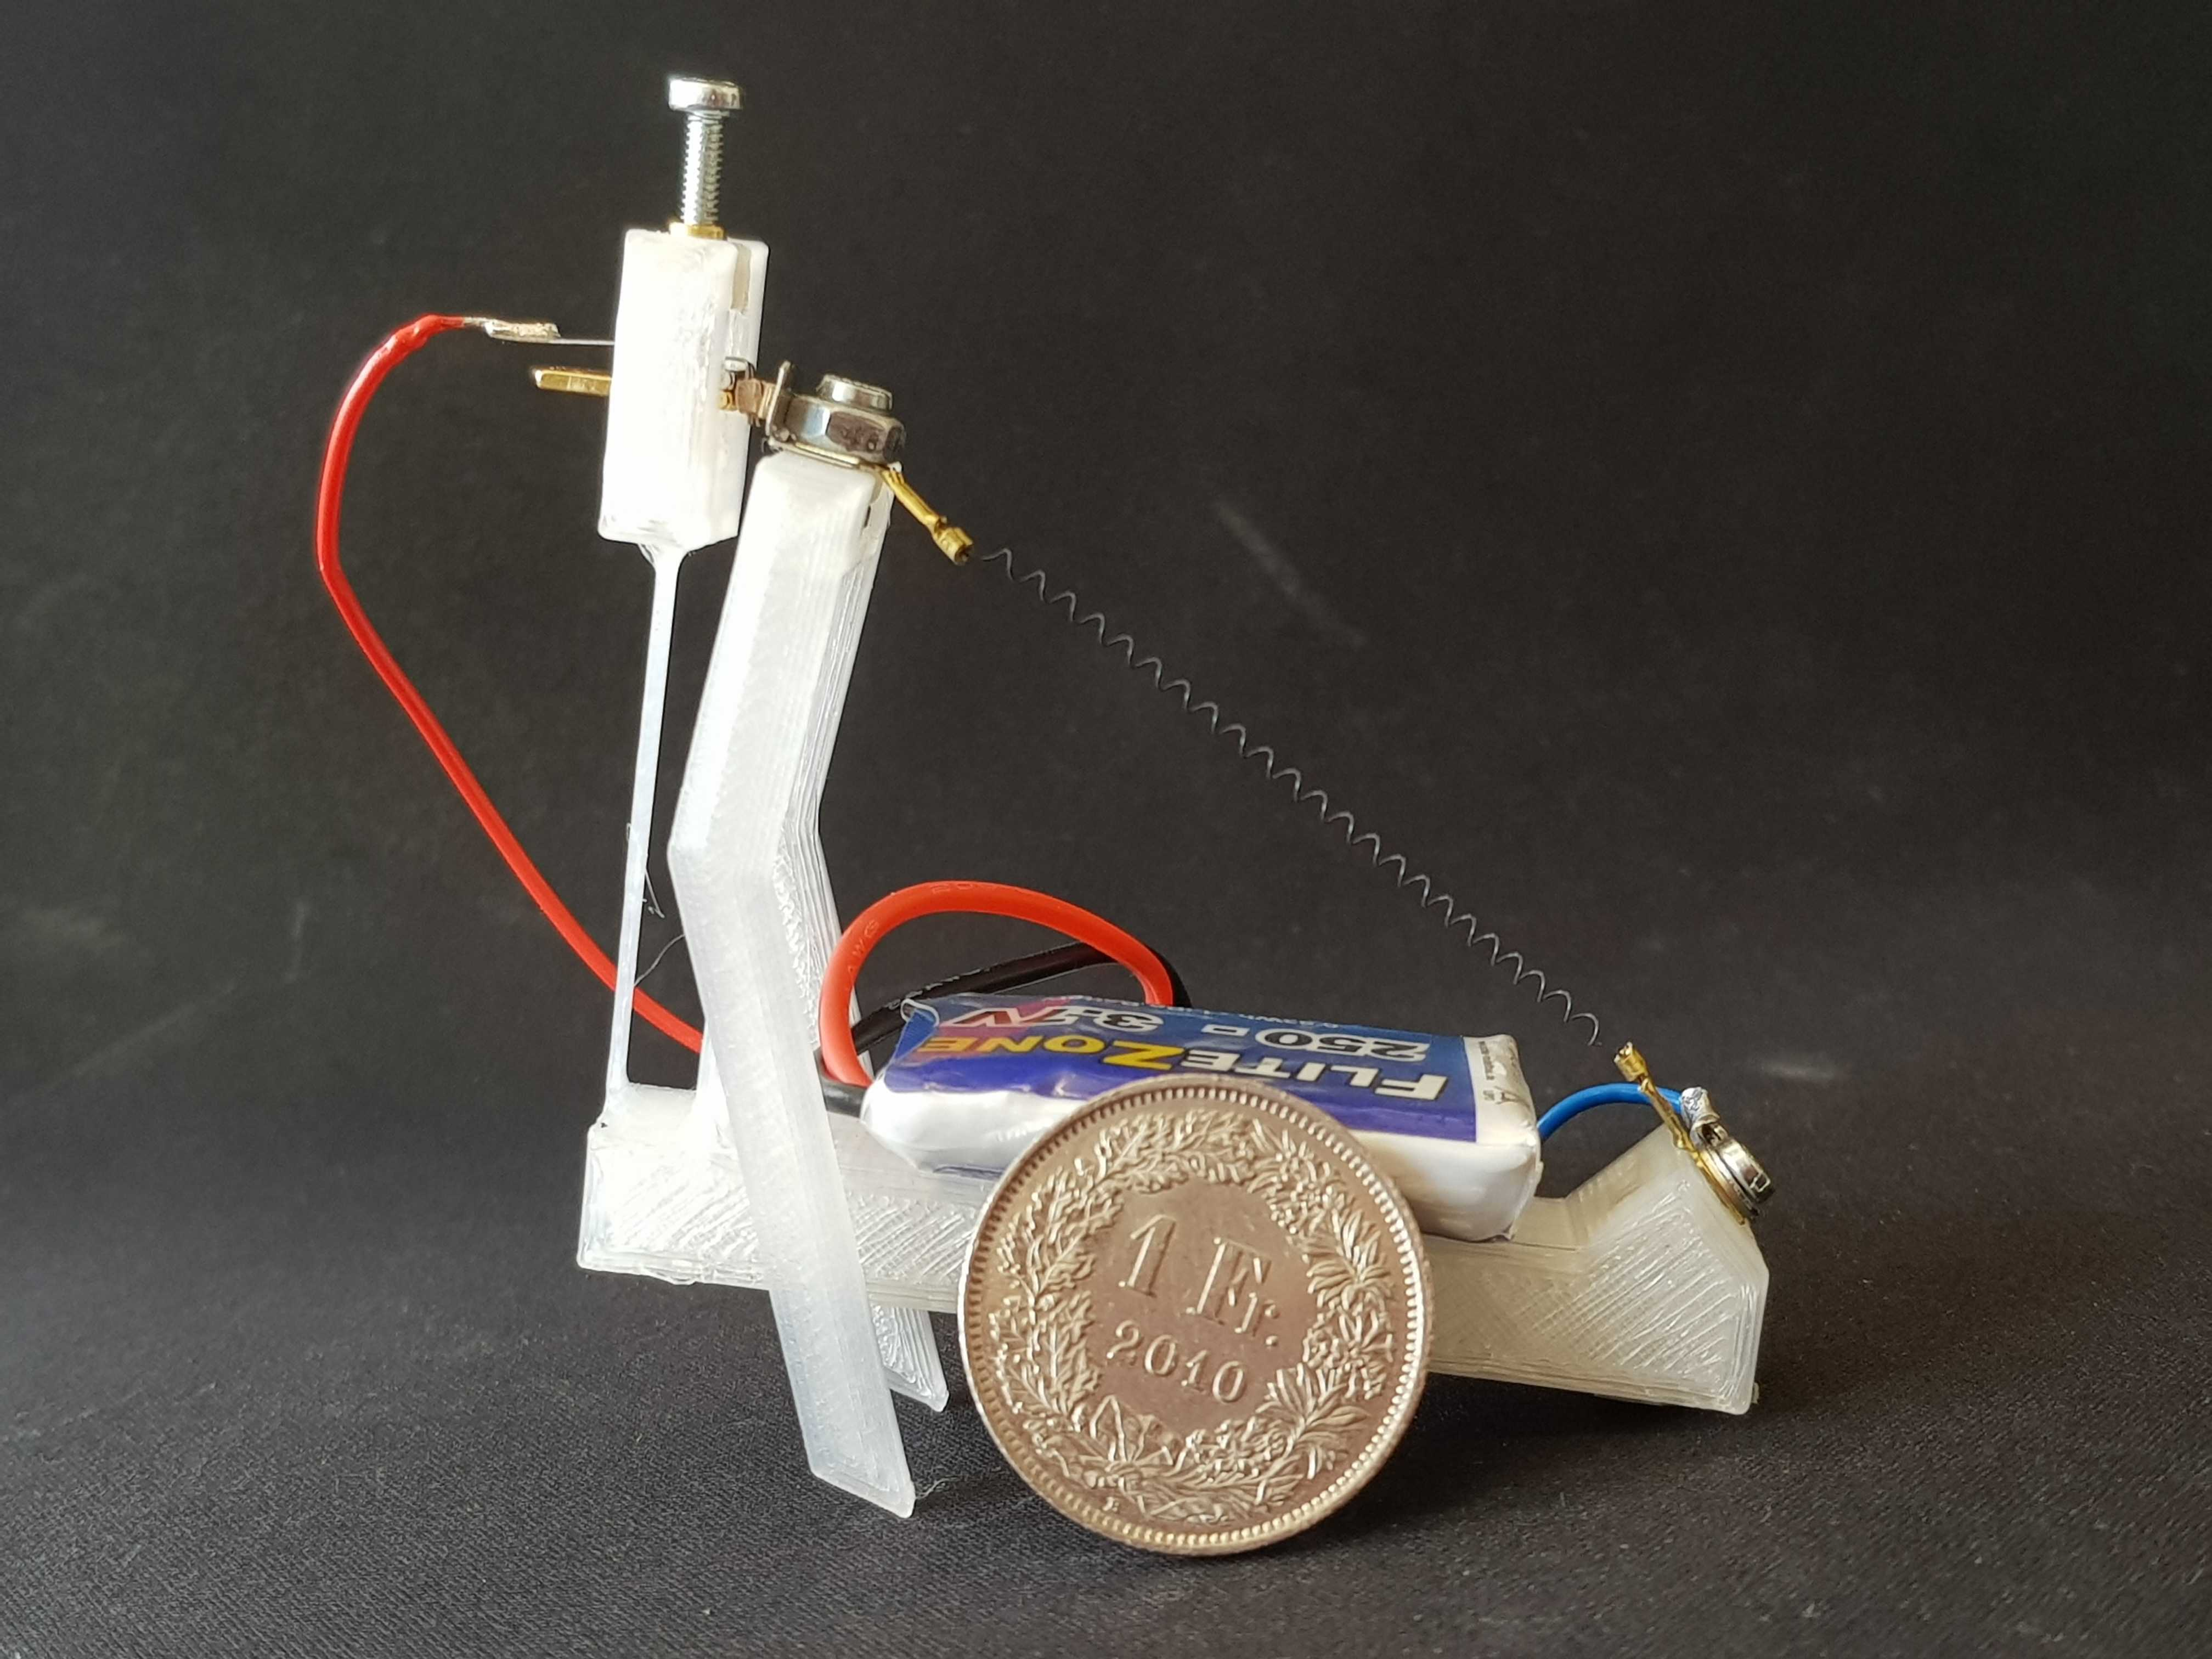
\includegraphics[trim={19cm 0cm 22cm 0cm},clip,width=0.7\textwidth]{images/chap6/insect-proto-bentleg.jpg}}
    	% \annotatedFigureBox{0.165,0.6493}{0.3111,0.9739}{A}{0.165,0.6493}{myblue}%bl
      % \node at (0.1595,0.8813) [fill=none,ultra thick,shape=circle,draw=white,inner sep=2pt,font=\sffamily,text=white, opacity=0.8] {\textbf{A}};
      \node [anchor=east, rotate=0] (ML) at (0.1895,0.8813) {\color{white} \normalsize \makecell[r]{Magnetic\\latch}};

      % \node at (0.1595,0.5313) [fill=none,ultra thick,shape=circle,draw=white,inner sep=2pt,font=\sffamily,text=white, opacity=0.8] {\textbf{B}};
      \node [anchor=east, rotate=82] (MLS) at (0.1855,0.663) {\color{white}Leaf spring};

    	% \node at (0.3755,0.6113) [fill=none,ultra thick,shape=circle,draw=black,inner sep=2pt,font=\sffamily,text=black, opacity=0.8] {\textbf{C}};
      \node [anchor=west, rotate=0] (SMALS) at (0.3605,0.5513) {\color{mygreen} \normalsize \makecell[l]{Bias\\leaf spring}};
      % \node [anchor=east, rotate=85] (SMALS) at (0.3405,0.6513) {\color{black} \footnotesize SMA leaf spring};

      % \node at (0.613,0.623) [fill=none,ultra thick,shape=circle,draw=white,inner sep=2pt,font=\sffamily,text=white, opacity=0.8] {\textbf{D}};
      \node [anchor=west, rotate=-42] (SMAC) at (0.613,0.623) {\color{white} SMA};

      % SMA Cantilever
      \node (sbot) at (0.26,0.31) {};
      \node (stop) at (0.33,0.69) {};
      \draw[dashed,ultra thick,color=mygreen] (sbot) to [bend left=8] (stop);
    \end{annotatedFigure}
    }{197.8}{2.2}{20}
%   \includegraphics[trim={3cm 5cm 3cm 3cm},clip, width=0.75\textwidth]{img/transducer.jpg}

    % \begin{tabular}{r@{ }l r@{ }l}
    %     A : & Magnetic latch & B : & Magnet cantilever leaf spring\\
    %     C : & SMA coil & D : & SMA cantilever leaf spring\\
    % \end{tabular}
    \caption{The implementation of the insect robot around the mechanical SMA oscillator.}
    \label{fig:insect-proto-diagram}
\end{figure}

The insect robot operates in a similar manner to the inchworm presented in \cref{subsec:bio-analysis} where the claws alternate between high friction and low friction with respect to the ground. By activating its artificial abdominal muscle consisting of the SMA coil, the insect robot is able to crawl across the ground. Here, the alternating friction that occurs at the claws is due to the design of the tips of the insect legs. The angle of the legs as the robot moves changes the angle of contact with the ground surface. As the leg tip design is asymmetrical with the direction of movement, the rotation of the legs cause alternating high and low friction. The behaviour is similar to a ratchet system where one degree of freedom is allowed in the forward direction but not in the backward direction. Here, the claw design allows rotation in the clockwise direction but prevents some rotation in the anti-clockwise direction. As the SMA is heated, the insect robot moves its forelegs away from the body. Then, when the SMA coil is stretch by the biasing leaf spring during cooling, the forelegs grip the ground and drags the rest of the body along the ground. By repeatedly heating and cooling the SMA, the insect robot can gradually move across the ground. As detailed in this novel control strategy, the magnetic latch system allows the SMA to oscillate and control the steps of the insect robot without any micro-controllers or electronics.

\subsection{Analytical model of the Biasing Compliant Mechanism}

When sizing the design and SMA of the insect robot, an analytical model of the compliant mechanism is required. This models allows dimensioning the SMA coil such that sufficient stroke is observed during the shape memory effect. Here, the stroke of the SMA actuator or the contraction of the SMA coil corresponds to the estimated step length of the insect robot.

The crux of the design revolves around the flexure-based biasing element and kinematic stage which, in this design, consists of a simple cantilever leaf spring. This flexural structure converts the linear contraction of the SMA coil into the rotation of the insect legs while also serving as the bias spring for SMA actuator allowing the coil to be stretched during the cooling phase based on the design approach detailed in \cref{chap:design-methodology}.

\begin{figure}[hbt!] % t for top of the page, H could be put to impose the position of the float
   \centering
   \begin{tikzpicture}
     \begin{scope}[x={(graph.south east)},y={(graph.north west)}]
       \coordinate (P) at (0.295,0.56);
       \coordinate (P0) at (0.17,0.65);
       \coordinate (S) at (0.55,0.16);
       \coordinate (V) at (0.145,0.33);
       \coordinate (C) at (0.058,0.02);
         \node[anchor=south west,inner sep=0] (image) at (0,0) {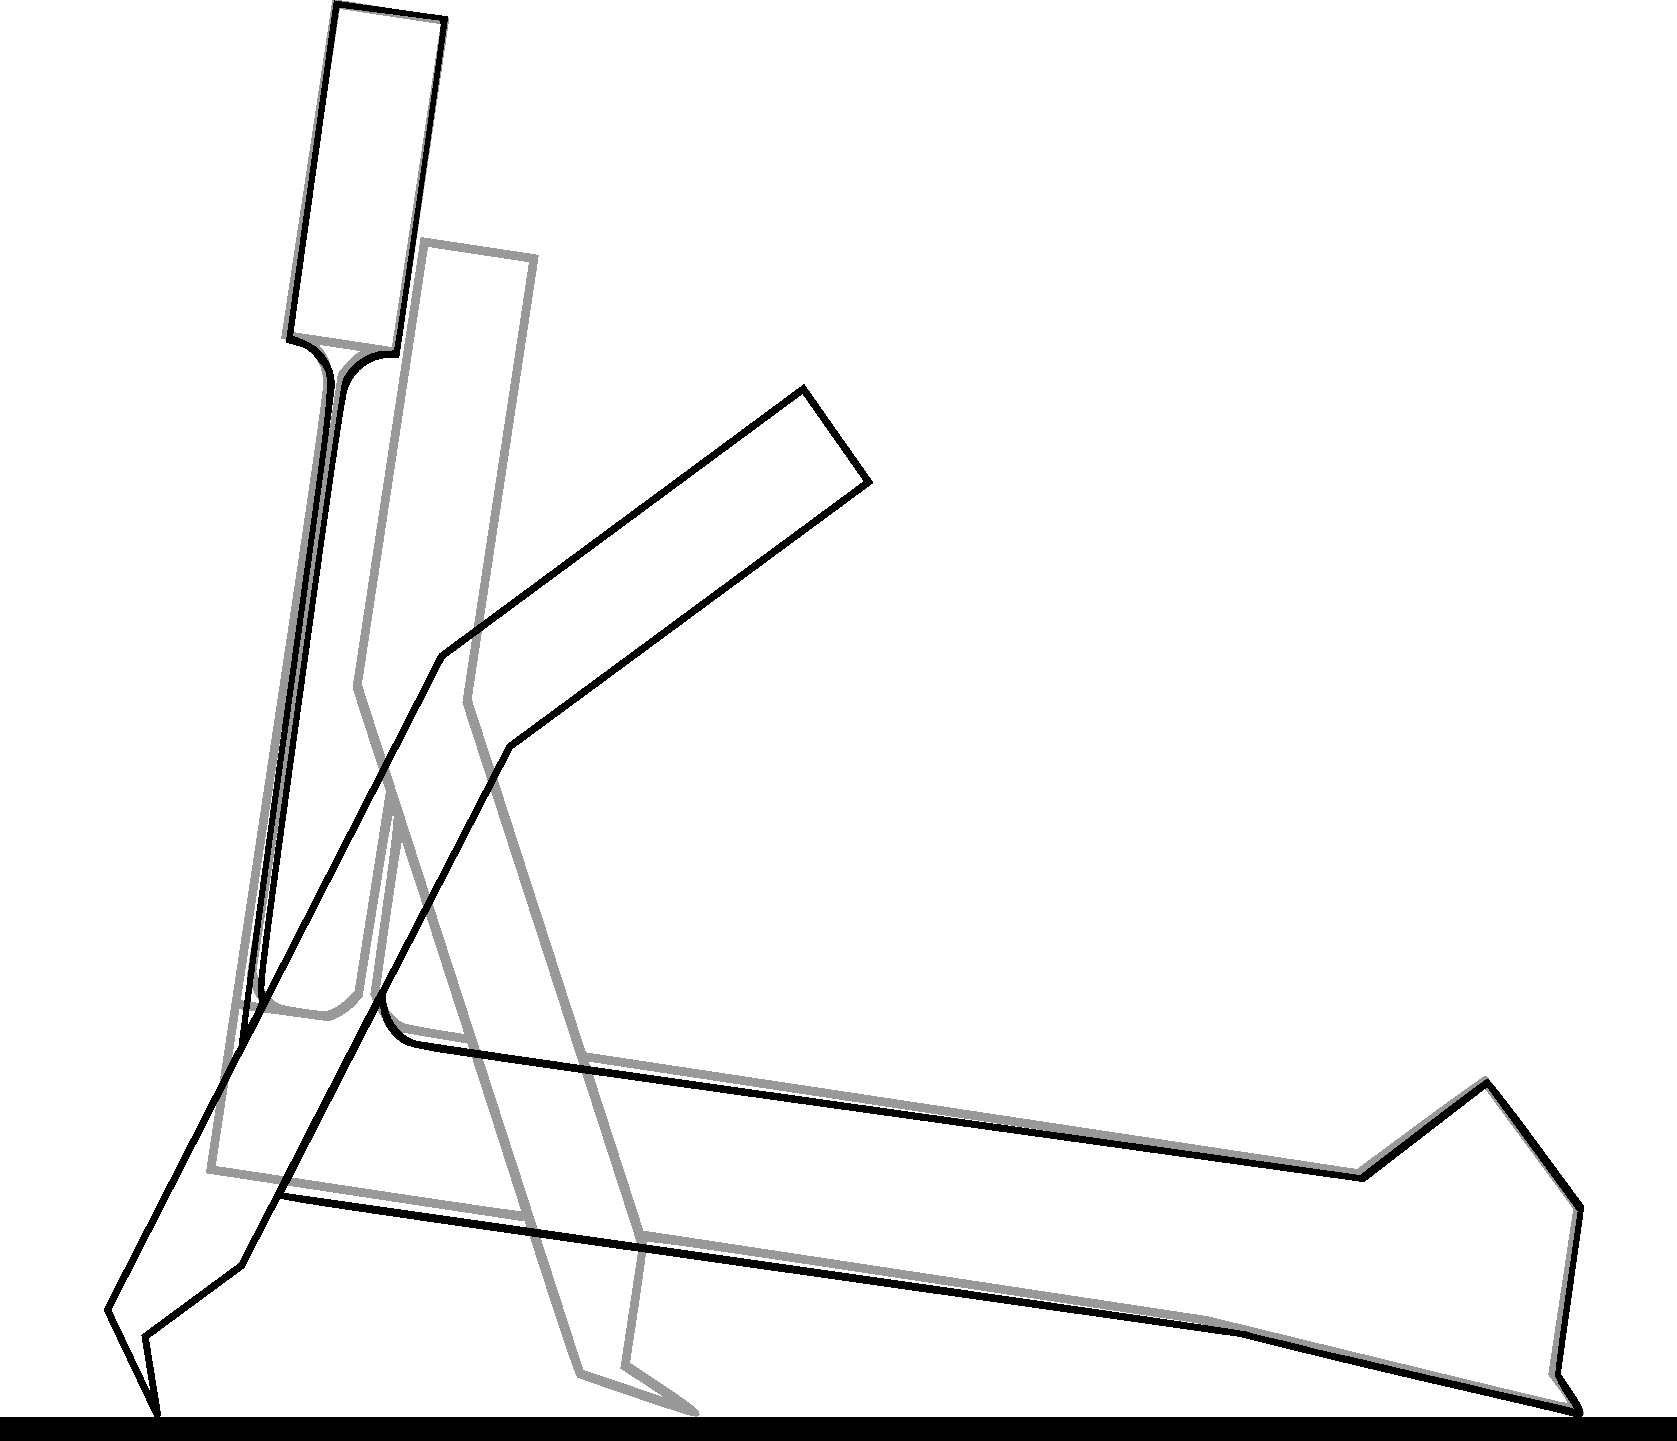
\includegraphics[trim={0 0cm 0 0cm},clip, width=0.5\textwidth]{images/chap6/insect-walking-diagram.pdf}};
         \node [anchor=west] (hfrictext) at (-0.030,0.05) {$\uparrow\mu_s$};
         \node [anchor=west] (lfrictext) at (0.25,0.05) {$\downarrow\mu_s$};
         \filldraw[black] (P) circle (2pt) node[anchor=south east,shift={(-0.02,0)}] {\normalsize P};
         \filldraw[black] (S) circle (2pt) node[anchor=north] {\normalsize S};
         \filldraw[black] (V) circle (2pt) node[anchor=north west,shift={(0.015,0)}] {\normalsize V};
         \filldraw[black] (C) circle (2pt) node[label={[shift={(0.02,-0.02)}]\normalsize C}] {};
         \draw[decoration={aspect=0.3, segment length=1mm, amplitude=0.3mm,coil},decorate] (P) -- node[above, rotate = -42] {\normalsize$r_2$} (S);
         \draw[decoration={aspect=0.3, segment length=1mm, amplitude=0.3mm,coil},decorate, opacity=0.5] (P0) -- node[below, rotate = -40,opacity=0.5] {\normalsize $L'_{SMA}$} (S);
         % \draw[dashed] (P) -- (S);

         % For claw only figure
         % \node [anchor=west, rotate=-62] (lfrictext) at (2.4,2.1) {\footnotesize Low friction};
         % \node [anchor=west, rotate=70] (hfrictext) at (0,0.3) {\footnotesize High friction};
         % Grid
         % \draw[lightgray,step=0.1] (image.south west) grid (image.north east);
         % \foreach \x in {0,0.1,...,1} { \node [below, rotate=-90] at (\x,0) {\tiny \x}; }
	     %    \foreach \y in {0,0.1,...,1} { \node [left] at (0,\y) {\tiny \y};}
     \end{scope}
     % \draw [brown] (current bounding box.south west) rectangle (current bounding box.north east);
   \end{tikzpicture}%
   ~
   \resizebox{0.3\textwidth}{!}{
   \begin{tikzpicture}
     \coordinate (rigid-top) at (0.75,1.5);
     \coordinate (deflected-top) at (0.5,0.65);
     \coordinate (top) at (0,1.5);
     \coordinate (bot) at (0,-1.5);
     \coordinate (virtual-pivot) at (0,-1);
     \filldraw[black] (virtual-pivot) circle (1pt) node[anchor=east] {V};
     \draw[line width=1.5mm] (-0.25,-1.5) -- (0.25,-1.5); % Ground
     \draw[dashed] (bot) -- (top);
     \draw[dashed] (virtual-pivot) -- (rigid-top);
     \draw[line width=0.5mm] (bot) to [bend left=5.5] (deflected-top); % cantilever
     \draw[line width=1mm] (deflected-top) -- (rigid-top); % rigid cantilever

     % Annotations
     \draw[|-|, line width=0.2mm] ($ (bot) + (0.6,0) $) -- node[anchor=west]{\scriptsize$aL$} ($ (virtual-pivot) + (0.6,0) $);
     \draw[|-|, line width=0.2mm] ($ (bot) + (-0.5,0) $) -- node[anchor=east]{\scriptsize$L$} ($ (0,0.65) + (-0.5,0) $);
     \draw[|-|, line width=0.2mm] ($ (deflected-top) + (0.5,-0.15) $) -- node[anchor=west]{\scriptsize$bL$} ($ (rigid-top) + (0.5,-0.15) $$);
     \draw (0,0.6) node[anchor=south west]{$\theta$} arc (90:76:2);
     % \dimline[line style = {line width=0.5}]{$ (bot) + (0.6,0) $}{$ (virtual-pivot) + (0.6,0) $}{$aL$};
     % \path ($ (bot) + (0.6,0) $) to[dim below=$aL$] ($ (virtual-pivot) + (0.6,0) $);
     % \path ($ (bot) + (-0.25,0) $) to[dim above=$L$] ($ (0,0.65) + (-0.25,0) $);
     % \path ($ (deflected-top) + (0.5,-0.15) $) to[dim below=$bL$] ($ (rigid-top) + (0.5,-0.15) $);
     % \pic ["$\theta$", draw, -, angle eccentricity=1.2, angle radius=1.5cm] {angle = deflected-top--virtual-pivot--top};
   \end{tikzpicture}%
   }
  \caption{The working principle of the insect robot showing the simplification of the cantilever beam to a virtual rigid body pivot. The claw design changes the coefficient of friction ($\mu_s$) of the insect with respect to the ground allowing the robot to crawl.}
  \label{fig:insect-claw-diagram}
\end{figure}

The pseudo-rigid-body model, as described in the work by \cite{howellHandbookCompliantMechanisms2013}, is used to model flexure-based mechanisms such as the cantilever beam as traditional rigid-body mechanisms. Thus, by simplifying the cantilever leaf spring as a virtual pivot, an analytical model can be established to estimate the effect of the SMA coil contraction. In the work by \cite{zhangRealPivotStructure2007}, the location of the virtual pivot can be estimated with relative accuracy to a point at a distance of $aL$ from the clamped end of the cantilever beam, where $L$ is the length of the beam, $bL$ is the length of the rigid attachment point with the SMA coil and $a$ is:

\begin{equation}\label{eq:virtual-pivot-a}
a = \frac{1+3b}{3+6b}
\end{equation}

The pre-stretched SMA coil of length, $L'_{SMA}$, is attached to the biasing cantilever leaf spring at the free end as shown in \cref{fig:insect-claw-diagram}. The position of cantilever tip, $P(x_P,y_P)$, as the SMA coil contracts in length by $\varepsilon$, can be deduced by finding the intersection between the two circles with radii, $r_1$ and $r_2$, and with centres at the virtual pivot $V(x_V,y_V)$ and fixed end of the SMA coil $S(x_S,y_S)$, respectively.

\begin{equation}\label{eq:cc-intersect}
  P(x,y) = \frac{1}{2}\begin{pmatrix} x_V+x_S \\ y_V+y_S \end{pmatrix}+\frac{r_1^2-r_2^2}{2R^2}\begin{pmatrix} x_S-x_V \\ y_S-y_V\end{pmatrix}\pm\frac{1}{2}\sqrt{2\frac{r_1^2+r_2^2}{R^2}-\frac{(r_1^2-r_2^2)^2}{R^4}-1}\begin{pmatrix} y_S-y_V \\ x_V-x_S\end{pmatrix}
\end{equation}
where $R$ is the Euclidean distance, $|\overline{VS}|$, between the two circle centres, $r_1 = (1-a+b)L$ and $r_2 = L'_{SMA}-\varepsilon$ representing the current length of the SMA coil.

As the insect legs are attached at the cantilever tip, the claw tips, $C(x_C,y_C)$, of the insect robot can be estimated by using a series of simple translation and rotation transformations from the cantilever tip based on the angles ($\alpha$) and lengths ($L$) of the insect leg segments.

\begin{equation}\label{eq:C}
  C(x,y) = \begin{pmatrix} x_P \\ y_P \end{pmatrix} + \sum_{i=1}L_i\begin{pmatrix} \cos(-\frac{\pi}{2}-\theta+\sum_{i=1}\alpha_i) \\ \sin(-\frac{\pi}{2}-\theta+\sum_{i=1}\alpha_i) \end{pmatrix}
\end{equation}
% \begin{multline}\label{eq:C}
%   \qquad C(x,y) = \begin{pmatrix} x_P \\ y_P \end{pmatrix} \\+ \sum_{i=1}L_i\begin{pmatrix} \cos(-\frac{\pi}{2}-\theta+\sum_{i=1}\alpha_i) \\ \sin(-\frac{\pi}{2}-\theta+\sum_{i=1}\alpha_i) \end{pmatrix}
% \end{multline}

Thus, based on the contraction or strain recovery of the SMA coil ($\varepsilon$), the step length of the insect, $\Delta C$, can be estimated by taking the Euclidean distance between the claw tip location before and after the SMA contraction. The position of the insect robot claw and the step length based on the SMA coil contraction can be seen in \cref{fig:insect-am-fem-compare}.

\begin{figure}[hb!] % t for top of the page, H could be put to impose the position of the float
  \centering
  \resizebox{0.95\columnwidth}{!}{%% Creator: Matplotlib, PGF backend
%%
%% To include the figure in your LaTeX document, write
%%   \input{<filename>.pgf}
%%
%% Make sure the required packages are loaded in your preamble
%%   \usepackage{pgf}
%%
%% and, on pdftex
%%   \usepackage[utf8]{inputenc}\DeclareUnicodeCharacter{2212}{-}
%%
%% or, on luatex and xetex
%%   \usepackage{unicode-math}
%%
%% Figures using additional raster images can only be included by \input if
%% they are in the same directory as the main LaTeX file. For loading figures
%% from other directories you can use the `import` package
%%   \usepackage{import}
%%
%% and then include the figures with
%%   \import{<path to file>}{<filename>.pgf}
%%
%% Matplotlib used the following preamble
%%
\begingroup%
\makeatletter%
\begin{pgfpicture}%
\pgfpathrectangle{\pgfpointorigin}{\pgfqpoint{4.528026in}{4.359349in}}%
\pgfusepath{use as bounding box, clip}%
\begin{pgfscope}%
\pgfsetbuttcap%
\pgfsetmiterjoin%
\pgfsetlinewidth{0.000000pt}%
\definecolor{currentstroke}{rgb}{0.000000,0.000000,0.000000}%
\pgfsetstrokecolor{currentstroke}%
\pgfsetstrokeopacity{0.000000}%
\pgfsetdash{}{0pt}%
\pgfpathmoveto{\pgfqpoint{0.000000in}{0.000000in}}%
\pgfpathlineto{\pgfqpoint{4.528026in}{0.000000in}}%
\pgfpathlineto{\pgfqpoint{4.528026in}{4.359349in}}%
\pgfpathlineto{\pgfqpoint{0.000000in}{4.359349in}}%
\pgfpathclose%
\pgfusepath{}%
\end{pgfscope}%
\begin{pgfscope}%
\pgfsetbuttcap%
\pgfsetmiterjoin%
\pgfsetlinewidth{0.000000pt}%
\definecolor{currentstroke}{rgb}{0.000000,0.000000,0.000000}%
\pgfsetstrokecolor{currentstroke}%
\pgfsetstrokeopacity{0.000000}%
\pgfsetdash{}{0pt}%
\pgfpathmoveto{\pgfqpoint{0.638581in}{2.531123in}}%
\pgfpathlineto{\pgfqpoint{4.358581in}{2.531123in}}%
\pgfpathlineto{\pgfqpoint{4.358581in}{4.211123in}}%
\pgfpathlineto{\pgfqpoint{0.638581in}{4.211123in}}%
\pgfpathclose%
\pgfusepath{}%
\end{pgfscope}%
\begin{pgfscope}%
\pgfpathrectangle{\pgfqpoint{0.638581in}{2.531123in}}{\pgfqpoint{3.720000in}{1.680000in}}%
\pgfusepath{clip}%
\pgfsetbuttcap%
\pgfsetroundjoin%
\pgfsetlinewidth{0.803000pt}%
\definecolor{currentstroke}{rgb}{0.690196,0.690196,0.690196}%
\pgfsetstrokecolor{currentstroke}%
\pgfsetstrokeopacity{0.800000}%
\pgfsetdash{{0.800000pt}{1.320000pt}}{0.000000pt}%
\pgfpathmoveto{\pgfqpoint{0.638581in}{2.531123in}}%
\pgfpathlineto{\pgfqpoint{0.638581in}{4.211123in}}%
\pgfusepath{stroke}%
\end{pgfscope}%
\begin{pgfscope}%
\pgfsetbuttcap%
\pgfsetroundjoin%
\definecolor{currentfill}{rgb}{0.000000,0.000000,0.000000}%
\pgfsetfillcolor{currentfill}%
\pgfsetlinewidth{0.803000pt}%
\definecolor{currentstroke}{rgb}{0.000000,0.000000,0.000000}%
\pgfsetstrokecolor{currentstroke}%
\pgfsetdash{}{0pt}%
\pgfsys@defobject{currentmarker}{\pgfqpoint{0.000000in}{-0.048611in}}{\pgfqpoint{0.000000in}{0.000000in}}{%
\pgfpathmoveto{\pgfqpoint{0.000000in}{0.000000in}}%
\pgfpathlineto{\pgfqpoint{0.000000in}{-0.048611in}}%
\pgfusepath{stroke,fill}%
}%
\begin{pgfscope}%
\pgfsys@transformshift{0.638581in}{2.531123in}%
\pgfsys@useobject{currentmarker}{}%
\end{pgfscope}%
\end{pgfscope}%
\begin{pgfscope}%
\definecolor{textcolor}{rgb}{0.000000,0.000000,0.000000}%
\pgfsetstrokecolor{textcolor}%
\pgfsetfillcolor{textcolor}%
\pgftext[x=0.638581in,y=2.433901in,,top]{\color{textcolor}\rmfamily\fontsize{10.000000}{12.000000}\selectfont \(\displaystyle {0}\)}%
\end{pgfscope}%
\begin{pgfscope}%
\pgfpathrectangle{\pgfqpoint{0.638581in}{2.531123in}}{\pgfqpoint{3.720000in}{1.680000in}}%
\pgfusepath{clip}%
\pgfsetbuttcap%
\pgfsetroundjoin%
\pgfsetlinewidth{0.803000pt}%
\definecolor{currentstroke}{rgb}{0.690196,0.690196,0.690196}%
\pgfsetstrokecolor{currentstroke}%
\pgfsetstrokeopacity{0.800000}%
\pgfsetdash{{0.800000pt}{1.320000pt}}{0.000000pt}%
\pgfpathmoveto{\pgfqpoint{1.382581in}{2.531123in}}%
\pgfpathlineto{\pgfqpoint{1.382581in}{4.211123in}}%
\pgfusepath{stroke}%
\end{pgfscope}%
\begin{pgfscope}%
\pgfsetbuttcap%
\pgfsetroundjoin%
\definecolor{currentfill}{rgb}{0.000000,0.000000,0.000000}%
\pgfsetfillcolor{currentfill}%
\pgfsetlinewidth{0.803000pt}%
\definecolor{currentstroke}{rgb}{0.000000,0.000000,0.000000}%
\pgfsetstrokecolor{currentstroke}%
\pgfsetdash{}{0pt}%
\pgfsys@defobject{currentmarker}{\pgfqpoint{0.000000in}{-0.048611in}}{\pgfqpoint{0.000000in}{0.000000in}}{%
\pgfpathmoveto{\pgfqpoint{0.000000in}{0.000000in}}%
\pgfpathlineto{\pgfqpoint{0.000000in}{-0.048611in}}%
\pgfusepath{stroke,fill}%
}%
\begin{pgfscope}%
\pgfsys@transformshift{1.382581in}{2.531123in}%
\pgfsys@useobject{currentmarker}{}%
\end{pgfscope}%
\end{pgfscope}%
\begin{pgfscope}%
\definecolor{textcolor}{rgb}{0.000000,0.000000,0.000000}%
\pgfsetstrokecolor{textcolor}%
\pgfsetfillcolor{textcolor}%
\pgftext[x=1.382581in,y=2.433901in,,top]{\color{textcolor}\rmfamily\fontsize{10.000000}{12.000000}\selectfont \(\displaystyle {2}\)}%
\end{pgfscope}%
\begin{pgfscope}%
\pgfpathrectangle{\pgfqpoint{0.638581in}{2.531123in}}{\pgfqpoint{3.720000in}{1.680000in}}%
\pgfusepath{clip}%
\pgfsetbuttcap%
\pgfsetroundjoin%
\pgfsetlinewidth{0.803000pt}%
\definecolor{currentstroke}{rgb}{0.690196,0.690196,0.690196}%
\pgfsetstrokecolor{currentstroke}%
\pgfsetstrokeopacity{0.800000}%
\pgfsetdash{{0.800000pt}{1.320000pt}}{0.000000pt}%
\pgfpathmoveto{\pgfqpoint{2.126581in}{2.531123in}}%
\pgfpathlineto{\pgfqpoint{2.126581in}{4.211123in}}%
\pgfusepath{stroke}%
\end{pgfscope}%
\begin{pgfscope}%
\pgfsetbuttcap%
\pgfsetroundjoin%
\definecolor{currentfill}{rgb}{0.000000,0.000000,0.000000}%
\pgfsetfillcolor{currentfill}%
\pgfsetlinewidth{0.803000pt}%
\definecolor{currentstroke}{rgb}{0.000000,0.000000,0.000000}%
\pgfsetstrokecolor{currentstroke}%
\pgfsetdash{}{0pt}%
\pgfsys@defobject{currentmarker}{\pgfqpoint{0.000000in}{-0.048611in}}{\pgfqpoint{0.000000in}{0.000000in}}{%
\pgfpathmoveto{\pgfqpoint{0.000000in}{0.000000in}}%
\pgfpathlineto{\pgfqpoint{0.000000in}{-0.048611in}}%
\pgfusepath{stroke,fill}%
}%
\begin{pgfscope}%
\pgfsys@transformshift{2.126581in}{2.531123in}%
\pgfsys@useobject{currentmarker}{}%
\end{pgfscope}%
\end{pgfscope}%
\begin{pgfscope}%
\definecolor{textcolor}{rgb}{0.000000,0.000000,0.000000}%
\pgfsetstrokecolor{textcolor}%
\pgfsetfillcolor{textcolor}%
\pgftext[x=2.126581in,y=2.433901in,,top]{\color{textcolor}\rmfamily\fontsize{10.000000}{12.000000}\selectfont \(\displaystyle {4}\)}%
\end{pgfscope}%
\begin{pgfscope}%
\pgfpathrectangle{\pgfqpoint{0.638581in}{2.531123in}}{\pgfqpoint{3.720000in}{1.680000in}}%
\pgfusepath{clip}%
\pgfsetbuttcap%
\pgfsetroundjoin%
\pgfsetlinewidth{0.803000pt}%
\definecolor{currentstroke}{rgb}{0.690196,0.690196,0.690196}%
\pgfsetstrokecolor{currentstroke}%
\pgfsetstrokeopacity{0.800000}%
\pgfsetdash{{0.800000pt}{1.320000pt}}{0.000000pt}%
\pgfpathmoveto{\pgfqpoint{2.870581in}{2.531123in}}%
\pgfpathlineto{\pgfqpoint{2.870581in}{4.211123in}}%
\pgfusepath{stroke}%
\end{pgfscope}%
\begin{pgfscope}%
\pgfsetbuttcap%
\pgfsetroundjoin%
\definecolor{currentfill}{rgb}{0.000000,0.000000,0.000000}%
\pgfsetfillcolor{currentfill}%
\pgfsetlinewidth{0.803000pt}%
\definecolor{currentstroke}{rgb}{0.000000,0.000000,0.000000}%
\pgfsetstrokecolor{currentstroke}%
\pgfsetdash{}{0pt}%
\pgfsys@defobject{currentmarker}{\pgfqpoint{0.000000in}{-0.048611in}}{\pgfqpoint{0.000000in}{0.000000in}}{%
\pgfpathmoveto{\pgfqpoint{0.000000in}{0.000000in}}%
\pgfpathlineto{\pgfqpoint{0.000000in}{-0.048611in}}%
\pgfusepath{stroke,fill}%
}%
\begin{pgfscope}%
\pgfsys@transformshift{2.870581in}{2.531123in}%
\pgfsys@useobject{currentmarker}{}%
\end{pgfscope}%
\end{pgfscope}%
\begin{pgfscope}%
\definecolor{textcolor}{rgb}{0.000000,0.000000,0.000000}%
\pgfsetstrokecolor{textcolor}%
\pgfsetfillcolor{textcolor}%
\pgftext[x=2.870581in,y=2.433901in,,top]{\color{textcolor}\rmfamily\fontsize{10.000000}{12.000000}\selectfont \(\displaystyle {6}\)}%
\end{pgfscope}%
\begin{pgfscope}%
\pgfpathrectangle{\pgfqpoint{0.638581in}{2.531123in}}{\pgfqpoint{3.720000in}{1.680000in}}%
\pgfusepath{clip}%
\pgfsetbuttcap%
\pgfsetroundjoin%
\pgfsetlinewidth{0.803000pt}%
\definecolor{currentstroke}{rgb}{0.690196,0.690196,0.690196}%
\pgfsetstrokecolor{currentstroke}%
\pgfsetstrokeopacity{0.800000}%
\pgfsetdash{{0.800000pt}{1.320000pt}}{0.000000pt}%
\pgfpathmoveto{\pgfqpoint{3.614581in}{2.531123in}}%
\pgfpathlineto{\pgfqpoint{3.614581in}{4.211123in}}%
\pgfusepath{stroke}%
\end{pgfscope}%
\begin{pgfscope}%
\pgfsetbuttcap%
\pgfsetroundjoin%
\definecolor{currentfill}{rgb}{0.000000,0.000000,0.000000}%
\pgfsetfillcolor{currentfill}%
\pgfsetlinewidth{0.803000pt}%
\definecolor{currentstroke}{rgb}{0.000000,0.000000,0.000000}%
\pgfsetstrokecolor{currentstroke}%
\pgfsetdash{}{0pt}%
\pgfsys@defobject{currentmarker}{\pgfqpoint{0.000000in}{-0.048611in}}{\pgfqpoint{0.000000in}{0.000000in}}{%
\pgfpathmoveto{\pgfqpoint{0.000000in}{0.000000in}}%
\pgfpathlineto{\pgfqpoint{0.000000in}{-0.048611in}}%
\pgfusepath{stroke,fill}%
}%
\begin{pgfscope}%
\pgfsys@transformshift{3.614581in}{2.531123in}%
\pgfsys@useobject{currentmarker}{}%
\end{pgfscope}%
\end{pgfscope}%
\begin{pgfscope}%
\definecolor{textcolor}{rgb}{0.000000,0.000000,0.000000}%
\pgfsetstrokecolor{textcolor}%
\pgfsetfillcolor{textcolor}%
\pgftext[x=3.614581in,y=2.433901in,,top]{\color{textcolor}\rmfamily\fontsize{10.000000}{12.000000}\selectfont \(\displaystyle {8}\)}%
\end{pgfscope}%
\begin{pgfscope}%
\pgfpathrectangle{\pgfqpoint{0.638581in}{2.531123in}}{\pgfqpoint{3.720000in}{1.680000in}}%
\pgfusepath{clip}%
\pgfsetbuttcap%
\pgfsetroundjoin%
\pgfsetlinewidth{0.803000pt}%
\definecolor{currentstroke}{rgb}{0.690196,0.690196,0.690196}%
\pgfsetstrokecolor{currentstroke}%
\pgfsetstrokeopacity{0.800000}%
\pgfsetdash{{0.800000pt}{1.320000pt}}{0.000000pt}%
\pgfpathmoveto{\pgfqpoint{4.358581in}{2.531123in}}%
\pgfpathlineto{\pgfqpoint{4.358581in}{4.211123in}}%
\pgfusepath{stroke}%
\end{pgfscope}%
\begin{pgfscope}%
\pgfsetbuttcap%
\pgfsetroundjoin%
\definecolor{currentfill}{rgb}{0.000000,0.000000,0.000000}%
\pgfsetfillcolor{currentfill}%
\pgfsetlinewidth{0.803000pt}%
\definecolor{currentstroke}{rgb}{0.000000,0.000000,0.000000}%
\pgfsetstrokecolor{currentstroke}%
\pgfsetdash{}{0pt}%
\pgfsys@defobject{currentmarker}{\pgfqpoint{0.000000in}{-0.048611in}}{\pgfqpoint{0.000000in}{0.000000in}}{%
\pgfpathmoveto{\pgfqpoint{0.000000in}{0.000000in}}%
\pgfpathlineto{\pgfqpoint{0.000000in}{-0.048611in}}%
\pgfusepath{stroke,fill}%
}%
\begin{pgfscope}%
\pgfsys@transformshift{4.358581in}{2.531123in}%
\pgfsys@useobject{currentmarker}{}%
\end{pgfscope}%
\end{pgfscope}%
\begin{pgfscope}%
\definecolor{textcolor}{rgb}{0.000000,0.000000,0.000000}%
\pgfsetstrokecolor{textcolor}%
\pgfsetfillcolor{textcolor}%
\pgftext[x=4.358581in,y=2.433901in,,top]{\color{textcolor}\rmfamily\fontsize{10.000000}{12.000000}\selectfont \(\displaystyle {10}\)}%
\end{pgfscope}%
\begin{pgfscope}%
\pgfpathrectangle{\pgfqpoint{0.638581in}{2.531123in}}{\pgfqpoint{3.720000in}{1.680000in}}%
\pgfusepath{clip}%
\pgfsetbuttcap%
\pgfsetroundjoin%
\pgfsetlinewidth{0.803000pt}%
\definecolor{currentstroke}{rgb}{0.690196,0.690196,0.690196}%
\pgfsetstrokecolor{currentstroke}%
\pgfsetstrokeopacity{0.800000}%
\pgfsetdash{{0.800000pt}{1.320000pt}}{0.000000pt}%
\pgfpathmoveto{\pgfqpoint{0.638581in}{2.531123in}}%
\pgfpathlineto{\pgfqpoint{4.358581in}{2.531123in}}%
\pgfusepath{stroke}%
\end{pgfscope}%
\begin{pgfscope}%
\pgfsetbuttcap%
\pgfsetroundjoin%
\definecolor{currentfill}{rgb}{0.000000,0.000000,0.000000}%
\pgfsetfillcolor{currentfill}%
\pgfsetlinewidth{0.803000pt}%
\definecolor{currentstroke}{rgb}{0.000000,0.000000,0.000000}%
\pgfsetstrokecolor{currentstroke}%
\pgfsetdash{}{0pt}%
\pgfsys@defobject{currentmarker}{\pgfqpoint{-0.048611in}{0.000000in}}{\pgfqpoint{-0.000000in}{0.000000in}}{%
\pgfpathmoveto{\pgfqpoint{-0.000000in}{0.000000in}}%
\pgfpathlineto{\pgfqpoint{-0.048611in}{0.000000in}}%
\pgfusepath{stroke,fill}%
}%
\begin{pgfscope}%
\pgfsys@transformshift{0.638581in}{2.531123in}%
\pgfsys@useobject{currentmarker}{}%
\end{pgfscope}%
\end{pgfscope}%
\begin{pgfscope}%
\definecolor{textcolor}{rgb}{0.000000,0.000000,0.000000}%
\pgfsetstrokecolor{textcolor}%
\pgfsetfillcolor{textcolor}%
\pgftext[x=0.363889in, y=2.482898in, left, base]{\color{textcolor}\rmfamily\fontsize{10.000000}{12.000000}\selectfont \(\displaystyle {0.0}\)}%
\end{pgfscope}%
\begin{pgfscope}%
\pgfpathrectangle{\pgfqpoint{0.638581in}{2.531123in}}{\pgfqpoint{3.720000in}{1.680000in}}%
\pgfusepath{clip}%
\pgfsetbuttcap%
\pgfsetroundjoin%
\pgfsetlinewidth{0.803000pt}%
\definecolor{currentstroke}{rgb}{0.690196,0.690196,0.690196}%
\pgfsetstrokecolor{currentstroke}%
\pgfsetstrokeopacity{0.800000}%
\pgfsetdash{{0.800000pt}{1.320000pt}}{0.000000pt}%
\pgfpathmoveto{\pgfqpoint{0.638581in}{2.811123in}}%
\pgfpathlineto{\pgfqpoint{4.358581in}{2.811123in}}%
\pgfusepath{stroke}%
\end{pgfscope}%
\begin{pgfscope}%
\pgfsetbuttcap%
\pgfsetroundjoin%
\definecolor{currentfill}{rgb}{0.000000,0.000000,0.000000}%
\pgfsetfillcolor{currentfill}%
\pgfsetlinewidth{0.803000pt}%
\definecolor{currentstroke}{rgb}{0.000000,0.000000,0.000000}%
\pgfsetstrokecolor{currentstroke}%
\pgfsetdash{}{0pt}%
\pgfsys@defobject{currentmarker}{\pgfqpoint{-0.048611in}{0.000000in}}{\pgfqpoint{-0.000000in}{0.000000in}}{%
\pgfpathmoveto{\pgfqpoint{-0.000000in}{0.000000in}}%
\pgfpathlineto{\pgfqpoint{-0.048611in}{0.000000in}}%
\pgfusepath{stroke,fill}%
}%
\begin{pgfscope}%
\pgfsys@transformshift{0.638581in}{2.811123in}%
\pgfsys@useobject{currentmarker}{}%
\end{pgfscope}%
\end{pgfscope}%
\begin{pgfscope}%
\definecolor{textcolor}{rgb}{0.000000,0.000000,0.000000}%
\pgfsetstrokecolor{textcolor}%
\pgfsetfillcolor{textcolor}%
\pgftext[x=0.363889in, y=2.762898in, left, base]{\color{textcolor}\rmfamily\fontsize{10.000000}{12.000000}\selectfont \(\displaystyle {2.5}\)}%
\end{pgfscope}%
\begin{pgfscope}%
\pgfpathrectangle{\pgfqpoint{0.638581in}{2.531123in}}{\pgfqpoint{3.720000in}{1.680000in}}%
\pgfusepath{clip}%
\pgfsetbuttcap%
\pgfsetroundjoin%
\pgfsetlinewidth{0.803000pt}%
\definecolor{currentstroke}{rgb}{0.690196,0.690196,0.690196}%
\pgfsetstrokecolor{currentstroke}%
\pgfsetstrokeopacity{0.800000}%
\pgfsetdash{{0.800000pt}{1.320000pt}}{0.000000pt}%
\pgfpathmoveto{\pgfqpoint{0.638581in}{3.091123in}}%
\pgfpathlineto{\pgfqpoint{4.358581in}{3.091123in}}%
\pgfusepath{stroke}%
\end{pgfscope}%
\begin{pgfscope}%
\pgfsetbuttcap%
\pgfsetroundjoin%
\definecolor{currentfill}{rgb}{0.000000,0.000000,0.000000}%
\pgfsetfillcolor{currentfill}%
\pgfsetlinewidth{0.803000pt}%
\definecolor{currentstroke}{rgb}{0.000000,0.000000,0.000000}%
\pgfsetstrokecolor{currentstroke}%
\pgfsetdash{}{0pt}%
\pgfsys@defobject{currentmarker}{\pgfqpoint{-0.048611in}{0.000000in}}{\pgfqpoint{-0.000000in}{0.000000in}}{%
\pgfpathmoveto{\pgfqpoint{-0.000000in}{0.000000in}}%
\pgfpathlineto{\pgfqpoint{-0.048611in}{0.000000in}}%
\pgfusepath{stroke,fill}%
}%
\begin{pgfscope}%
\pgfsys@transformshift{0.638581in}{3.091123in}%
\pgfsys@useobject{currentmarker}{}%
\end{pgfscope}%
\end{pgfscope}%
\begin{pgfscope}%
\definecolor{textcolor}{rgb}{0.000000,0.000000,0.000000}%
\pgfsetstrokecolor{textcolor}%
\pgfsetfillcolor{textcolor}%
\pgftext[x=0.363889in, y=3.042898in, left, base]{\color{textcolor}\rmfamily\fontsize{10.000000}{12.000000}\selectfont \(\displaystyle {5.0}\)}%
\end{pgfscope}%
\begin{pgfscope}%
\pgfpathrectangle{\pgfqpoint{0.638581in}{2.531123in}}{\pgfqpoint{3.720000in}{1.680000in}}%
\pgfusepath{clip}%
\pgfsetbuttcap%
\pgfsetroundjoin%
\pgfsetlinewidth{0.803000pt}%
\definecolor{currentstroke}{rgb}{0.690196,0.690196,0.690196}%
\pgfsetstrokecolor{currentstroke}%
\pgfsetstrokeopacity{0.800000}%
\pgfsetdash{{0.800000pt}{1.320000pt}}{0.000000pt}%
\pgfpathmoveto{\pgfqpoint{0.638581in}{3.371123in}}%
\pgfpathlineto{\pgfqpoint{4.358581in}{3.371123in}}%
\pgfusepath{stroke}%
\end{pgfscope}%
\begin{pgfscope}%
\pgfsetbuttcap%
\pgfsetroundjoin%
\definecolor{currentfill}{rgb}{0.000000,0.000000,0.000000}%
\pgfsetfillcolor{currentfill}%
\pgfsetlinewidth{0.803000pt}%
\definecolor{currentstroke}{rgb}{0.000000,0.000000,0.000000}%
\pgfsetstrokecolor{currentstroke}%
\pgfsetdash{}{0pt}%
\pgfsys@defobject{currentmarker}{\pgfqpoint{-0.048611in}{0.000000in}}{\pgfqpoint{-0.000000in}{0.000000in}}{%
\pgfpathmoveto{\pgfqpoint{-0.000000in}{0.000000in}}%
\pgfpathlineto{\pgfqpoint{-0.048611in}{0.000000in}}%
\pgfusepath{stroke,fill}%
}%
\begin{pgfscope}%
\pgfsys@transformshift{0.638581in}{3.371123in}%
\pgfsys@useobject{currentmarker}{}%
\end{pgfscope}%
\end{pgfscope}%
\begin{pgfscope}%
\definecolor{textcolor}{rgb}{0.000000,0.000000,0.000000}%
\pgfsetstrokecolor{textcolor}%
\pgfsetfillcolor{textcolor}%
\pgftext[x=0.363889in, y=3.322898in, left, base]{\color{textcolor}\rmfamily\fontsize{10.000000}{12.000000}\selectfont \(\displaystyle {7.5}\)}%
\end{pgfscope}%
\begin{pgfscope}%
\pgfpathrectangle{\pgfqpoint{0.638581in}{2.531123in}}{\pgfqpoint{3.720000in}{1.680000in}}%
\pgfusepath{clip}%
\pgfsetbuttcap%
\pgfsetroundjoin%
\pgfsetlinewidth{0.803000pt}%
\definecolor{currentstroke}{rgb}{0.690196,0.690196,0.690196}%
\pgfsetstrokecolor{currentstroke}%
\pgfsetstrokeopacity{0.800000}%
\pgfsetdash{{0.800000pt}{1.320000pt}}{0.000000pt}%
\pgfpathmoveto{\pgfqpoint{0.638581in}{3.651123in}}%
\pgfpathlineto{\pgfqpoint{4.358581in}{3.651123in}}%
\pgfusepath{stroke}%
\end{pgfscope}%
\begin{pgfscope}%
\pgfsetbuttcap%
\pgfsetroundjoin%
\definecolor{currentfill}{rgb}{0.000000,0.000000,0.000000}%
\pgfsetfillcolor{currentfill}%
\pgfsetlinewidth{0.803000pt}%
\definecolor{currentstroke}{rgb}{0.000000,0.000000,0.000000}%
\pgfsetstrokecolor{currentstroke}%
\pgfsetdash{}{0pt}%
\pgfsys@defobject{currentmarker}{\pgfqpoint{-0.048611in}{0.000000in}}{\pgfqpoint{-0.000000in}{0.000000in}}{%
\pgfpathmoveto{\pgfqpoint{-0.000000in}{0.000000in}}%
\pgfpathlineto{\pgfqpoint{-0.048611in}{0.000000in}}%
\pgfusepath{stroke,fill}%
}%
\begin{pgfscope}%
\pgfsys@transformshift{0.638581in}{3.651123in}%
\pgfsys@useobject{currentmarker}{}%
\end{pgfscope}%
\end{pgfscope}%
\begin{pgfscope}%
\definecolor{textcolor}{rgb}{0.000000,0.000000,0.000000}%
\pgfsetstrokecolor{textcolor}%
\pgfsetfillcolor{textcolor}%
\pgftext[x=0.294444in, y=3.602898in, left, base]{\color{textcolor}\rmfamily\fontsize{10.000000}{12.000000}\selectfont \(\displaystyle {10.0}\)}%
\end{pgfscope}%
\begin{pgfscope}%
\pgfpathrectangle{\pgfqpoint{0.638581in}{2.531123in}}{\pgfqpoint{3.720000in}{1.680000in}}%
\pgfusepath{clip}%
\pgfsetbuttcap%
\pgfsetroundjoin%
\pgfsetlinewidth{0.803000pt}%
\definecolor{currentstroke}{rgb}{0.690196,0.690196,0.690196}%
\pgfsetstrokecolor{currentstroke}%
\pgfsetstrokeopacity{0.800000}%
\pgfsetdash{{0.800000pt}{1.320000pt}}{0.000000pt}%
\pgfpathmoveto{\pgfqpoint{0.638581in}{3.931123in}}%
\pgfpathlineto{\pgfqpoint{4.358581in}{3.931123in}}%
\pgfusepath{stroke}%
\end{pgfscope}%
\begin{pgfscope}%
\pgfsetbuttcap%
\pgfsetroundjoin%
\definecolor{currentfill}{rgb}{0.000000,0.000000,0.000000}%
\pgfsetfillcolor{currentfill}%
\pgfsetlinewidth{0.803000pt}%
\definecolor{currentstroke}{rgb}{0.000000,0.000000,0.000000}%
\pgfsetstrokecolor{currentstroke}%
\pgfsetdash{}{0pt}%
\pgfsys@defobject{currentmarker}{\pgfqpoint{-0.048611in}{0.000000in}}{\pgfqpoint{-0.000000in}{0.000000in}}{%
\pgfpathmoveto{\pgfqpoint{-0.000000in}{0.000000in}}%
\pgfpathlineto{\pgfqpoint{-0.048611in}{0.000000in}}%
\pgfusepath{stroke,fill}%
}%
\begin{pgfscope}%
\pgfsys@transformshift{0.638581in}{3.931123in}%
\pgfsys@useobject{currentmarker}{}%
\end{pgfscope}%
\end{pgfscope}%
\begin{pgfscope}%
\definecolor{textcolor}{rgb}{0.000000,0.000000,0.000000}%
\pgfsetstrokecolor{textcolor}%
\pgfsetfillcolor{textcolor}%
\pgftext[x=0.294444in, y=3.882898in, left, base]{\color{textcolor}\rmfamily\fontsize{10.000000}{12.000000}\selectfont \(\displaystyle {12.5}\)}%
\end{pgfscope}%
\begin{pgfscope}%
\pgfpathrectangle{\pgfqpoint{0.638581in}{2.531123in}}{\pgfqpoint{3.720000in}{1.680000in}}%
\pgfusepath{clip}%
\pgfsetbuttcap%
\pgfsetroundjoin%
\pgfsetlinewidth{0.803000pt}%
\definecolor{currentstroke}{rgb}{0.690196,0.690196,0.690196}%
\pgfsetstrokecolor{currentstroke}%
\pgfsetstrokeopacity{0.800000}%
\pgfsetdash{{0.800000pt}{1.320000pt}}{0.000000pt}%
\pgfpathmoveto{\pgfqpoint{0.638581in}{4.211123in}}%
\pgfpathlineto{\pgfqpoint{4.358581in}{4.211123in}}%
\pgfusepath{stroke}%
\end{pgfscope}%
\begin{pgfscope}%
\pgfsetbuttcap%
\pgfsetroundjoin%
\definecolor{currentfill}{rgb}{0.000000,0.000000,0.000000}%
\pgfsetfillcolor{currentfill}%
\pgfsetlinewidth{0.803000pt}%
\definecolor{currentstroke}{rgb}{0.000000,0.000000,0.000000}%
\pgfsetstrokecolor{currentstroke}%
\pgfsetdash{}{0pt}%
\pgfsys@defobject{currentmarker}{\pgfqpoint{-0.048611in}{0.000000in}}{\pgfqpoint{-0.000000in}{0.000000in}}{%
\pgfpathmoveto{\pgfqpoint{-0.000000in}{0.000000in}}%
\pgfpathlineto{\pgfqpoint{-0.048611in}{0.000000in}}%
\pgfusepath{stroke,fill}%
}%
\begin{pgfscope}%
\pgfsys@transformshift{0.638581in}{4.211123in}%
\pgfsys@useobject{currentmarker}{}%
\end{pgfscope}%
\end{pgfscope}%
\begin{pgfscope}%
\definecolor{textcolor}{rgb}{0.000000,0.000000,0.000000}%
\pgfsetstrokecolor{textcolor}%
\pgfsetfillcolor{textcolor}%
\pgftext[x=0.294444in, y=4.162898in, left, base]{\color{textcolor}\rmfamily\fontsize{10.000000}{12.000000}\selectfont \(\displaystyle {15.0}\)}%
\end{pgfscope}%
\begin{pgfscope}%
\definecolor{textcolor}{rgb}{0.000000,0.000000,0.000000}%
\pgfsetstrokecolor{textcolor}%
\pgfsetfillcolor{textcolor}%
\pgftext[x=0.238889in,y=3.371123in,,bottom,rotate=90.000000]{\color{textcolor}\rmfamily\fontsize{10.000000}{12.000000}\bfseries\selectfont Claw Coordinate \(\displaystyle C\) [mm]}%
\end{pgfscope}%
\begin{pgfscope}%
\pgfpathrectangle{\pgfqpoint{0.638581in}{2.531123in}}{\pgfqpoint{3.720000in}{1.680000in}}%
\pgfusepath{clip}%
\pgfsetrectcap%
\pgfsetroundjoin%
\pgfsetlinewidth{1.505625pt}%
\definecolor{currentstroke}{rgb}{0.905882,0.207843,0.219608}%
\pgfsetstrokecolor{currentstroke}%
\pgfsetdash{}{0pt}%
\pgfpathmoveto{\pgfqpoint{0.638581in}{2.531123in}}%
\pgfpathlineto{\pgfqpoint{0.832693in}{2.596025in}}%
\pgfpathlineto{\pgfqpoint{1.024561in}{2.660950in}}%
\pgfpathlineto{\pgfqpoint{1.221267in}{2.728286in}}%
\pgfpathlineto{\pgfqpoint{1.422668in}{2.798017in}}%
\pgfpathlineto{\pgfqpoint{1.628629in}{2.870123in}}%
\pgfpathlineto{\pgfqpoint{1.839020in}{2.944582in}}%
\pgfpathlineto{\pgfqpoint{2.053717in}{3.021371in}}%
\pgfpathlineto{\pgfqpoint{2.272603in}{3.100462in}}%
\pgfpathlineto{\pgfqpoint{2.495568in}{3.181827in}}%
\pgfpathlineto{\pgfqpoint{2.722508in}{3.265435in}}%
\pgfpathlineto{\pgfqpoint{2.953329in}{3.351252in}}%
\pgfpathlineto{\pgfqpoint{3.194245in}{3.441618in}}%
\pgfpathlineto{\pgfqpoint{3.444965in}{3.536474in}}%
\pgfpathlineto{\pgfqpoint{3.699051in}{3.633394in}}%
\pgfpathlineto{\pgfqpoint{3.968636in}{3.737036in}}%
\pgfpathlineto{\pgfqpoint{4.247247in}{3.844951in}}%
\pgfpathlineto{\pgfqpoint{4.361914in}{3.889586in}}%
\pgfpathlineto{\pgfqpoint{4.361914in}{3.889586in}}%
\pgfusepath{stroke}%
\end{pgfscope}%
\begin{pgfscope}%
\pgfpathrectangle{\pgfqpoint{0.638581in}{2.531123in}}{\pgfqpoint{3.720000in}{1.680000in}}%
\pgfusepath{clip}%
\pgfsetbuttcap%
\pgfsetroundjoin%
\pgfsetlinewidth{1.505625pt}%
\definecolor{currentstroke}{rgb}{0.905882,0.207843,0.219608}%
\pgfsetstrokecolor{currentstroke}%
\pgfsetdash{{1.500000pt}{2.475000pt}}{0.000000pt}%
\pgfpathmoveto{\pgfqpoint{0.721831in}{2.561217in}}%
\pgfpathlineto{\pgfqpoint{0.806089in}{2.591872in}}%
\pgfpathlineto{\pgfqpoint{0.908526in}{2.629401in}}%
\pgfpathlineto{\pgfqpoint{1.012404in}{2.667741in}}%
\pgfpathlineto{\pgfqpoint{1.117680in}{2.706896in}}%
\pgfpathlineto{\pgfqpoint{1.224369in}{2.746858in}}%
\pgfpathlineto{\pgfqpoint{1.332435in}{2.787615in}}%
\pgfpathlineto{\pgfqpoint{1.441841in}{2.829167in}}%
\pgfpathlineto{\pgfqpoint{1.552585in}{2.871514in}}%
\pgfpathlineto{\pgfqpoint{1.664594in}{2.914634in}}%
\pgfpathlineto{\pgfqpoint{1.777868in}{2.958515in}}%
\pgfpathlineto{\pgfqpoint{1.892333in}{3.003147in}}%
\pgfpathlineto{\pgfqpoint{2.007987in}{3.048507in}}%
\pgfpathlineto{\pgfqpoint{2.124721in}{3.094562in}}%
\pgfpathlineto{\pgfqpoint{2.242533in}{3.141311in}}%
\pgfpathlineto{\pgfqpoint{2.361350in}{3.188720in}}%
\pgfpathlineto{\pgfqpoint{2.481134in}{3.236757in}}%
\pgfpathlineto{\pgfqpoint{2.601811in}{3.285387in}}%
\pgfpathlineto{\pgfqpoint{2.723306in}{3.334600in}}%
\pgfpathlineto{\pgfqpoint{2.845545in}{3.384339in}}%
\pgfpathlineto{\pgfqpoint{2.968491in}{3.434583in}}%
\pgfpathlineto{\pgfqpoint{3.092107in}{3.485307in}}%
\pgfpathlineto{\pgfqpoint{3.216206in}{3.536435in}}%
\pgfpathlineto{\pgfqpoint{3.340789in}{3.587944in}}%
\pgfpathlineto{\pgfqpoint{3.465744in}{3.639789in}}%
\pgfpathlineto{\pgfqpoint{3.591071in}{3.691891in}}%
\pgfpathlineto{\pgfqpoint{3.716621in}{3.744307in}}%
\pgfpathlineto{\pgfqpoint{3.842357in}{3.796947in}}%
\pgfpathlineto{\pgfqpoint{3.968204in}{3.849699in}}%
\pgfpathlineto{\pgfqpoint{4.094089in}{3.902675in}}%
\pgfpathlineto{\pgfqpoint{4.219899in}{3.955651in}}%
\pgfpathlineto{\pgfqpoint{4.345635in}{4.008627in}}%
\pgfpathlineto{\pgfqpoint{4.361914in}{4.015505in}}%
\pgfusepath{stroke}%
\end{pgfscope}%
\begin{pgfscope}%
\pgfpathrectangle{\pgfqpoint{0.638581in}{2.531123in}}{\pgfqpoint{3.720000in}{1.680000in}}%
\pgfusepath{clip}%
\pgfsetrectcap%
\pgfsetroundjoin%
\pgfsetlinewidth{1.505625pt}%
\definecolor{currentstroke}{rgb}{0.000000,0.447059,0.741176}%
\pgfsetstrokecolor{currentstroke}%
\pgfsetdash{}{0pt}%
\pgfpathmoveto{\pgfqpoint{0.638581in}{2.531123in}}%
\pgfpathlineto{\pgfqpoint{0.782587in}{2.558087in}}%
\pgfpathlineto{\pgfqpoint{0.925348in}{2.584042in}}%
\pgfpathlineto{\pgfqpoint{1.066903in}{2.609011in}}%
\pgfpathlineto{\pgfqpoint{1.207291in}{2.633013in}}%
\pgfpathlineto{\pgfqpoint{1.346547in}{2.656070in}}%
\pgfpathlineto{\pgfqpoint{1.484706in}{2.678200in}}%
\pgfpathlineto{\pgfqpoint{1.621802in}{2.699420in}}%
\pgfpathlineto{\pgfqpoint{1.757865in}{2.719749in}}%
\pgfpathlineto{\pgfqpoint{1.892926in}{2.739201in}}%
\pgfpathlineto{\pgfqpoint{2.027013in}{2.757793in}}%
\pgfpathlineto{\pgfqpoint{2.160155in}{2.775540in}}%
\pgfpathlineto{\pgfqpoint{2.298966in}{2.793280in}}%
\pgfpathlineto{\pgfqpoint{2.436793in}{2.810118in}}%
\pgfpathlineto{\pgfqpoint{2.573665in}{2.826071in}}%
\pgfpathlineto{\pgfqpoint{2.709609in}{2.841152in}}%
\pgfpathlineto{\pgfqpoint{2.844651in}{2.855375in}}%
\pgfpathlineto{\pgfqpoint{2.978818in}{2.868753in}}%
\pgfpathlineto{\pgfqpoint{3.112133in}{2.881297in}}%
\pgfpathlineto{\pgfqpoint{3.244620in}{2.893021in}}%
\pgfpathlineto{\pgfqpoint{3.376302in}{2.903936in}}%
\pgfpathlineto{\pgfqpoint{3.507202in}{2.914051in}}%
\pgfpathlineto{\pgfqpoint{3.637341in}{2.923378in}}%
\pgfpathlineto{\pgfqpoint{3.766740in}{2.931926in}}%
\pgfpathlineto{\pgfqpoint{3.895420in}{2.939705in}}%
\pgfpathlineto{\pgfqpoint{4.023400in}{2.946724in}}%
\pgfpathlineto{\pgfqpoint{4.150701in}{2.952990in}}%
\pgfpathlineto{\pgfqpoint{4.277340in}{2.958512in}}%
\pgfpathlineto{\pgfqpoint{4.361914in}{2.961803in}}%
\pgfpathlineto{\pgfqpoint{4.361914in}{2.961803in}}%
\pgfusepath{stroke}%
\end{pgfscope}%
\begin{pgfscope}%
\pgfpathrectangle{\pgfqpoint{0.638581in}{2.531123in}}{\pgfqpoint{3.720000in}{1.680000in}}%
\pgfusepath{clip}%
\pgfsetbuttcap%
\pgfsetroundjoin%
\pgfsetlinewidth{1.505625pt}%
\definecolor{currentstroke}{rgb}{0.000000,0.447059,0.741176}%
\pgfsetstrokecolor{currentstroke}%
\pgfsetdash{{1.500000pt}{2.475000pt}}{0.000000pt}%
\pgfpathmoveto{\pgfqpoint{0.721831in}{2.550123in}}%
\pgfpathlineto{\pgfqpoint{0.806089in}{2.569010in}}%
\pgfpathlineto{\pgfqpoint{0.908526in}{2.591505in}}%
\pgfpathlineto{\pgfqpoint{1.012404in}{2.613787in}}%
\pgfpathlineto{\pgfqpoint{1.117680in}{2.635829in}}%
\pgfpathlineto{\pgfqpoint{1.224369in}{2.657605in}}%
\pgfpathlineto{\pgfqpoint{1.332435in}{2.679064in}}%
\pgfpathlineto{\pgfqpoint{1.441841in}{2.700210in}}%
\pgfpathlineto{\pgfqpoint{1.552585in}{2.720986in}}%
\pgfpathlineto{\pgfqpoint{1.664594in}{2.741359in}}%
\pgfpathlineto{\pgfqpoint{1.777868in}{2.761306in}}%
\pgfpathlineto{\pgfqpoint{1.892333in}{2.780805in}}%
\pgfpathlineto{\pgfqpoint{2.007987in}{2.799800in}}%
\pgfpathlineto{\pgfqpoint{2.124721in}{2.818269in}}%
\pgfpathlineto{\pgfqpoint{2.242533in}{2.836178in}}%
\pgfpathlineto{\pgfqpoint{2.361350in}{2.853504in}}%
\pgfpathlineto{\pgfqpoint{2.481134in}{2.870203in}}%
\pgfpathlineto{\pgfqpoint{2.601811in}{2.886253in}}%
\pgfpathlineto{\pgfqpoint{2.723306in}{2.901619in}}%
\pgfpathlineto{\pgfqpoint{2.845545in}{2.916280in}}%
\pgfpathlineto{\pgfqpoint{2.968491in}{2.930213in}}%
\pgfpathlineto{\pgfqpoint{3.092107in}{2.943395in}}%
\pgfpathlineto{\pgfqpoint{3.216206in}{2.955783in}}%
\pgfpathlineto{\pgfqpoint{3.340789in}{2.967363in}}%
\pgfpathlineto{\pgfqpoint{3.465744in}{2.978138in}}%
\pgfpathlineto{\pgfqpoint{3.591071in}{2.988061in}}%
\pgfpathlineto{\pgfqpoint{3.716621in}{2.997133in}}%
\pgfpathlineto{\pgfqpoint{3.842357in}{3.005331in}}%
\pgfpathlineto{\pgfqpoint{3.968204in}{3.012656in}}%
\pgfpathlineto{\pgfqpoint{4.094089in}{3.019096in}}%
\pgfpathlineto{\pgfqpoint{4.219899in}{3.024651in}}%
\pgfpathlineto{\pgfqpoint{4.345635in}{3.029299in}}%
\pgfpathlineto{\pgfqpoint{4.361914in}{3.029785in}}%
\pgfusepath{stroke}%
\end{pgfscope}%
\begin{pgfscope}%
\pgfsetrectcap%
\pgfsetmiterjoin%
\pgfsetlinewidth{0.803000pt}%
\definecolor{currentstroke}{rgb}{0.000000,0.000000,0.000000}%
\pgfsetstrokecolor{currentstroke}%
\pgfsetdash{}{0pt}%
\pgfpathmoveto{\pgfqpoint{0.638581in}{2.531123in}}%
\pgfpathlineto{\pgfqpoint{0.638581in}{4.211123in}}%
\pgfusepath{stroke}%
\end{pgfscope}%
\begin{pgfscope}%
\pgfsetrectcap%
\pgfsetmiterjoin%
\pgfsetlinewidth{0.803000pt}%
\definecolor{currentstroke}{rgb}{0.000000,0.000000,0.000000}%
\pgfsetstrokecolor{currentstroke}%
\pgfsetdash{}{0pt}%
\pgfpathmoveto{\pgfqpoint{4.358581in}{2.531123in}}%
\pgfpathlineto{\pgfqpoint{4.358581in}{4.211123in}}%
\pgfusepath{stroke}%
\end{pgfscope}%
\begin{pgfscope}%
\pgfsetrectcap%
\pgfsetmiterjoin%
\pgfsetlinewidth{0.803000pt}%
\definecolor{currentstroke}{rgb}{0.000000,0.000000,0.000000}%
\pgfsetstrokecolor{currentstroke}%
\pgfsetdash{}{0pt}%
\pgfpathmoveto{\pgfqpoint{0.638581in}{2.531123in}}%
\pgfpathlineto{\pgfqpoint{4.358581in}{2.531123in}}%
\pgfusepath{stroke}%
\end{pgfscope}%
\begin{pgfscope}%
\pgfsetrectcap%
\pgfsetmiterjoin%
\pgfsetlinewidth{0.803000pt}%
\definecolor{currentstroke}{rgb}{0.000000,0.000000,0.000000}%
\pgfsetstrokecolor{currentstroke}%
\pgfsetdash{}{0pt}%
\pgfpathmoveto{\pgfqpoint{0.638581in}{4.211123in}}%
\pgfpathlineto{\pgfqpoint{4.358581in}{4.211123in}}%
\pgfusepath{stroke}%
\end{pgfscope}%
\begin{pgfscope}%
\pgfsetbuttcap%
\pgfsetmiterjoin%
\definecolor{currentfill}{rgb}{1.000000,1.000000,1.000000}%
\pgfsetfillcolor{currentfill}%
\pgfsetfillopacity{0.800000}%
\pgfsetlinewidth{1.003750pt}%
\definecolor{currentstroke}{rgb}{0.800000,0.800000,0.800000}%
\pgfsetstrokecolor{currentstroke}%
\pgfsetstrokeopacity{0.800000}%
\pgfsetdash{}{0pt}%
\pgfpathmoveto{\pgfqpoint{0.735803in}{3.712667in}}%
\pgfpathlineto{\pgfqpoint{1.353043in}{3.712667in}}%
\pgfpathquadraticcurveto{\pgfqpoint{1.380821in}{3.712667in}}{\pgfqpoint{1.380821in}{3.740444in}}%
\pgfpathlineto{\pgfqpoint{1.380821in}{4.113901in}}%
\pgfpathquadraticcurveto{\pgfqpoint{1.380821in}{4.141679in}}{\pgfqpoint{1.353043in}{4.141679in}}%
\pgfpathlineto{\pgfqpoint{0.735803in}{4.141679in}}%
\pgfpathquadraticcurveto{\pgfqpoint{0.708025in}{4.141679in}}{\pgfqpoint{0.708025in}{4.113901in}}%
\pgfpathlineto{\pgfqpoint{0.708025in}{3.740444in}}%
\pgfpathquadraticcurveto{\pgfqpoint{0.708025in}{3.712667in}}{\pgfqpoint{0.735803in}{3.712667in}}%
\pgfpathclose%
\pgfusepath{stroke,fill}%
\end{pgfscope}%
\begin{pgfscope}%
\pgfsetrectcap%
\pgfsetroundjoin%
\pgfsetlinewidth{1.505625pt}%
\definecolor{currentstroke}{rgb}{0.905882,0.207843,0.219608}%
\pgfsetstrokecolor{currentstroke}%
\pgfsetdash{}{0pt}%
\pgfpathmoveto{\pgfqpoint{0.763581in}{4.037512in}}%
\pgfpathlineto{\pgfqpoint{1.041359in}{4.037512in}}%
\pgfusepath{stroke}%
\end{pgfscope}%
\begin{pgfscope}%
\definecolor{textcolor}{rgb}{0.000000,0.000000,0.000000}%
\pgfsetstrokecolor{textcolor}%
\pgfsetfillcolor{textcolor}%
\pgftext[x=1.152470in,y=3.988901in,left,base]{\color{textcolor}\rmfamily\fontsize{10.000000}{12.000000}\selectfont \(\displaystyle x_C\)}%
\end{pgfscope}%
\begin{pgfscope}%
\pgfsetrectcap%
\pgfsetroundjoin%
\pgfsetlinewidth{1.505625pt}%
\definecolor{currentstroke}{rgb}{0.000000,0.447059,0.741176}%
\pgfsetstrokecolor{currentstroke}%
\pgfsetdash{}{0pt}%
\pgfpathmoveto{\pgfqpoint{0.763581in}{3.843839in}}%
\pgfpathlineto{\pgfqpoint{1.041359in}{3.843839in}}%
\pgfusepath{stroke}%
\end{pgfscope}%
\begin{pgfscope}%
\definecolor{textcolor}{rgb}{0.000000,0.000000,0.000000}%
\pgfsetstrokecolor{textcolor}%
\pgfsetfillcolor{textcolor}%
\pgftext[x=1.152470in,y=3.795228in,left,base]{\color{textcolor}\rmfamily\fontsize{10.000000}{12.000000}\selectfont \(\displaystyle y_C\)}%
\end{pgfscope}%
\begin{pgfscope}%
\pgfsetbuttcap%
\pgfsetmiterjoin%
\pgfsetlinewidth{0.000000pt}%
\definecolor{currentstroke}{rgb}{0.000000,0.000000,0.000000}%
\pgfsetstrokecolor{currentstroke}%
\pgfsetstrokeopacity{0.000000}%
\pgfsetdash{}{0pt}%
\pgfpathmoveto{\pgfqpoint{0.638581in}{0.515123in}}%
\pgfpathlineto{\pgfqpoint{4.358581in}{0.515123in}}%
\pgfpathlineto{\pgfqpoint{4.358581in}{2.195123in}}%
\pgfpathlineto{\pgfqpoint{0.638581in}{2.195123in}}%
\pgfpathclose%
\pgfusepath{}%
\end{pgfscope}%
\begin{pgfscope}%
\pgfpathrectangle{\pgfqpoint{0.638581in}{0.515123in}}{\pgfqpoint{3.720000in}{1.680000in}}%
\pgfusepath{clip}%
\pgfsetbuttcap%
\pgfsetroundjoin%
\pgfsetlinewidth{0.803000pt}%
\definecolor{currentstroke}{rgb}{0.690196,0.690196,0.690196}%
\pgfsetstrokecolor{currentstroke}%
\pgfsetstrokeopacity{0.800000}%
\pgfsetdash{{0.800000pt}{1.320000pt}}{0.000000pt}%
\pgfpathmoveto{\pgfqpoint{0.638581in}{0.515123in}}%
\pgfpathlineto{\pgfqpoint{0.638581in}{2.195123in}}%
\pgfusepath{stroke}%
\end{pgfscope}%
\begin{pgfscope}%
\pgfsetbuttcap%
\pgfsetroundjoin%
\definecolor{currentfill}{rgb}{0.000000,0.000000,0.000000}%
\pgfsetfillcolor{currentfill}%
\pgfsetlinewidth{0.803000pt}%
\definecolor{currentstroke}{rgb}{0.000000,0.000000,0.000000}%
\pgfsetstrokecolor{currentstroke}%
\pgfsetdash{}{0pt}%
\pgfsys@defobject{currentmarker}{\pgfqpoint{0.000000in}{-0.048611in}}{\pgfqpoint{0.000000in}{0.000000in}}{%
\pgfpathmoveto{\pgfqpoint{0.000000in}{0.000000in}}%
\pgfpathlineto{\pgfqpoint{0.000000in}{-0.048611in}}%
\pgfusepath{stroke,fill}%
}%
\begin{pgfscope}%
\pgfsys@transformshift{0.638581in}{0.515123in}%
\pgfsys@useobject{currentmarker}{}%
\end{pgfscope}%
\end{pgfscope}%
\begin{pgfscope}%
\definecolor{textcolor}{rgb}{0.000000,0.000000,0.000000}%
\pgfsetstrokecolor{textcolor}%
\pgfsetfillcolor{textcolor}%
\pgftext[x=0.638581in,y=0.417901in,,top]{\color{textcolor}\rmfamily\fontsize{10.000000}{12.000000}\selectfont \(\displaystyle {0}\)}%
\end{pgfscope}%
\begin{pgfscope}%
\pgfpathrectangle{\pgfqpoint{0.638581in}{0.515123in}}{\pgfqpoint{3.720000in}{1.680000in}}%
\pgfusepath{clip}%
\pgfsetbuttcap%
\pgfsetroundjoin%
\pgfsetlinewidth{0.803000pt}%
\definecolor{currentstroke}{rgb}{0.690196,0.690196,0.690196}%
\pgfsetstrokecolor{currentstroke}%
\pgfsetstrokeopacity{0.800000}%
\pgfsetdash{{0.800000pt}{1.320000pt}}{0.000000pt}%
\pgfpathmoveto{\pgfqpoint{1.382581in}{0.515123in}}%
\pgfpathlineto{\pgfqpoint{1.382581in}{2.195123in}}%
\pgfusepath{stroke}%
\end{pgfscope}%
\begin{pgfscope}%
\pgfsetbuttcap%
\pgfsetroundjoin%
\definecolor{currentfill}{rgb}{0.000000,0.000000,0.000000}%
\pgfsetfillcolor{currentfill}%
\pgfsetlinewidth{0.803000pt}%
\definecolor{currentstroke}{rgb}{0.000000,0.000000,0.000000}%
\pgfsetstrokecolor{currentstroke}%
\pgfsetdash{}{0pt}%
\pgfsys@defobject{currentmarker}{\pgfqpoint{0.000000in}{-0.048611in}}{\pgfqpoint{0.000000in}{0.000000in}}{%
\pgfpathmoveto{\pgfqpoint{0.000000in}{0.000000in}}%
\pgfpathlineto{\pgfqpoint{0.000000in}{-0.048611in}}%
\pgfusepath{stroke,fill}%
}%
\begin{pgfscope}%
\pgfsys@transformshift{1.382581in}{0.515123in}%
\pgfsys@useobject{currentmarker}{}%
\end{pgfscope}%
\end{pgfscope}%
\begin{pgfscope}%
\definecolor{textcolor}{rgb}{0.000000,0.000000,0.000000}%
\pgfsetstrokecolor{textcolor}%
\pgfsetfillcolor{textcolor}%
\pgftext[x=1.382581in,y=0.417901in,,top]{\color{textcolor}\rmfamily\fontsize{10.000000}{12.000000}\selectfont \(\displaystyle {2}\)}%
\end{pgfscope}%
\begin{pgfscope}%
\pgfpathrectangle{\pgfqpoint{0.638581in}{0.515123in}}{\pgfqpoint{3.720000in}{1.680000in}}%
\pgfusepath{clip}%
\pgfsetbuttcap%
\pgfsetroundjoin%
\pgfsetlinewidth{0.803000pt}%
\definecolor{currentstroke}{rgb}{0.690196,0.690196,0.690196}%
\pgfsetstrokecolor{currentstroke}%
\pgfsetstrokeopacity{0.800000}%
\pgfsetdash{{0.800000pt}{1.320000pt}}{0.000000pt}%
\pgfpathmoveto{\pgfqpoint{2.126581in}{0.515123in}}%
\pgfpathlineto{\pgfqpoint{2.126581in}{2.195123in}}%
\pgfusepath{stroke}%
\end{pgfscope}%
\begin{pgfscope}%
\pgfsetbuttcap%
\pgfsetroundjoin%
\definecolor{currentfill}{rgb}{0.000000,0.000000,0.000000}%
\pgfsetfillcolor{currentfill}%
\pgfsetlinewidth{0.803000pt}%
\definecolor{currentstroke}{rgb}{0.000000,0.000000,0.000000}%
\pgfsetstrokecolor{currentstroke}%
\pgfsetdash{}{0pt}%
\pgfsys@defobject{currentmarker}{\pgfqpoint{0.000000in}{-0.048611in}}{\pgfqpoint{0.000000in}{0.000000in}}{%
\pgfpathmoveto{\pgfqpoint{0.000000in}{0.000000in}}%
\pgfpathlineto{\pgfqpoint{0.000000in}{-0.048611in}}%
\pgfusepath{stroke,fill}%
}%
\begin{pgfscope}%
\pgfsys@transformshift{2.126581in}{0.515123in}%
\pgfsys@useobject{currentmarker}{}%
\end{pgfscope}%
\end{pgfscope}%
\begin{pgfscope}%
\definecolor{textcolor}{rgb}{0.000000,0.000000,0.000000}%
\pgfsetstrokecolor{textcolor}%
\pgfsetfillcolor{textcolor}%
\pgftext[x=2.126581in,y=0.417901in,,top]{\color{textcolor}\rmfamily\fontsize{10.000000}{12.000000}\selectfont \(\displaystyle {4}\)}%
\end{pgfscope}%
\begin{pgfscope}%
\pgfpathrectangle{\pgfqpoint{0.638581in}{0.515123in}}{\pgfqpoint{3.720000in}{1.680000in}}%
\pgfusepath{clip}%
\pgfsetbuttcap%
\pgfsetroundjoin%
\pgfsetlinewidth{0.803000pt}%
\definecolor{currentstroke}{rgb}{0.690196,0.690196,0.690196}%
\pgfsetstrokecolor{currentstroke}%
\pgfsetstrokeopacity{0.800000}%
\pgfsetdash{{0.800000pt}{1.320000pt}}{0.000000pt}%
\pgfpathmoveto{\pgfqpoint{2.870581in}{0.515123in}}%
\pgfpathlineto{\pgfqpoint{2.870581in}{2.195123in}}%
\pgfusepath{stroke}%
\end{pgfscope}%
\begin{pgfscope}%
\pgfsetbuttcap%
\pgfsetroundjoin%
\definecolor{currentfill}{rgb}{0.000000,0.000000,0.000000}%
\pgfsetfillcolor{currentfill}%
\pgfsetlinewidth{0.803000pt}%
\definecolor{currentstroke}{rgb}{0.000000,0.000000,0.000000}%
\pgfsetstrokecolor{currentstroke}%
\pgfsetdash{}{0pt}%
\pgfsys@defobject{currentmarker}{\pgfqpoint{0.000000in}{-0.048611in}}{\pgfqpoint{0.000000in}{0.000000in}}{%
\pgfpathmoveto{\pgfqpoint{0.000000in}{0.000000in}}%
\pgfpathlineto{\pgfqpoint{0.000000in}{-0.048611in}}%
\pgfusepath{stroke,fill}%
}%
\begin{pgfscope}%
\pgfsys@transformshift{2.870581in}{0.515123in}%
\pgfsys@useobject{currentmarker}{}%
\end{pgfscope}%
\end{pgfscope}%
\begin{pgfscope}%
\definecolor{textcolor}{rgb}{0.000000,0.000000,0.000000}%
\pgfsetstrokecolor{textcolor}%
\pgfsetfillcolor{textcolor}%
\pgftext[x=2.870581in,y=0.417901in,,top]{\color{textcolor}\rmfamily\fontsize{10.000000}{12.000000}\selectfont \(\displaystyle {6}\)}%
\end{pgfscope}%
\begin{pgfscope}%
\pgfpathrectangle{\pgfqpoint{0.638581in}{0.515123in}}{\pgfqpoint{3.720000in}{1.680000in}}%
\pgfusepath{clip}%
\pgfsetbuttcap%
\pgfsetroundjoin%
\pgfsetlinewidth{0.803000pt}%
\definecolor{currentstroke}{rgb}{0.690196,0.690196,0.690196}%
\pgfsetstrokecolor{currentstroke}%
\pgfsetstrokeopacity{0.800000}%
\pgfsetdash{{0.800000pt}{1.320000pt}}{0.000000pt}%
\pgfpathmoveto{\pgfqpoint{3.614581in}{0.515123in}}%
\pgfpathlineto{\pgfqpoint{3.614581in}{2.195123in}}%
\pgfusepath{stroke}%
\end{pgfscope}%
\begin{pgfscope}%
\pgfsetbuttcap%
\pgfsetroundjoin%
\definecolor{currentfill}{rgb}{0.000000,0.000000,0.000000}%
\pgfsetfillcolor{currentfill}%
\pgfsetlinewidth{0.803000pt}%
\definecolor{currentstroke}{rgb}{0.000000,0.000000,0.000000}%
\pgfsetstrokecolor{currentstroke}%
\pgfsetdash{}{0pt}%
\pgfsys@defobject{currentmarker}{\pgfqpoint{0.000000in}{-0.048611in}}{\pgfqpoint{0.000000in}{0.000000in}}{%
\pgfpathmoveto{\pgfqpoint{0.000000in}{0.000000in}}%
\pgfpathlineto{\pgfqpoint{0.000000in}{-0.048611in}}%
\pgfusepath{stroke,fill}%
}%
\begin{pgfscope}%
\pgfsys@transformshift{3.614581in}{0.515123in}%
\pgfsys@useobject{currentmarker}{}%
\end{pgfscope}%
\end{pgfscope}%
\begin{pgfscope}%
\definecolor{textcolor}{rgb}{0.000000,0.000000,0.000000}%
\pgfsetstrokecolor{textcolor}%
\pgfsetfillcolor{textcolor}%
\pgftext[x=3.614581in,y=0.417901in,,top]{\color{textcolor}\rmfamily\fontsize{10.000000}{12.000000}\selectfont \(\displaystyle {8}\)}%
\end{pgfscope}%
\begin{pgfscope}%
\pgfpathrectangle{\pgfqpoint{0.638581in}{0.515123in}}{\pgfqpoint{3.720000in}{1.680000in}}%
\pgfusepath{clip}%
\pgfsetbuttcap%
\pgfsetroundjoin%
\pgfsetlinewidth{0.803000pt}%
\definecolor{currentstroke}{rgb}{0.690196,0.690196,0.690196}%
\pgfsetstrokecolor{currentstroke}%
\pgfsetstrokeopacity{0.800000}%
\pgfsetdash{{0.800000pt}{1.320000pt}}{0.000000pt}%
\pgfpathmoveto{\pgfqpoint{4.358581in}{0.515123in}}%
\pgfpathlineto{\pgfqpoint{4.358581in}{2.195123in}}%
\pgfusepath{stroke}%
\end{pgfscope}%
\begin{pgfscope}%
\pgfsetbuttcap%
\pgfsetroundjoin%
\definecolor{currentfill}{rgb}{0.000000,0.000000,0.000000}%
\pgfsetfillcolor{currentfill}%
\pgfsetlinewidth{0.803000pt}%
\definecolor{currentstroke}{rgb}{0.000000,0.000000,0.000000}%
\pgfsetstrokecolor{currentstroke}%
\pgfsetdash{}{0pt}%
\pgfsys@defobject{currentmarker}{\pgfqpoint{0.000000in}{-0.048611in}}{\pgfqpoint{0.000000in}{0.000000in}}{%
\pgfpathmoveto{\pgfqpoint{0.000000in}{0.000000in}}%
\pgfpathlineto{\pgfqpoint{0.000000in}{-0.048611in}}%
\pgfusepath{stroke,fill}%
}%
\begin{pgfscope}%
\pgfsys@transformshift{4.358581in}{0.515123in}%
\pgfsys@useobject{currentmarker}{}%
\end{pgfscope}%
\end{pgfscope}%
\begin{pgfscope}%
\definecolor{textcolor}{rgb}{0.000000,0.000000,0.000000}%
\pgfsetstrokecolor{textcolor}%
\pgfsetfillcolor{textcolor}%
\pgftext[x=4.358581in,y=0.417901in,,top]{\color{textcolor}\rmfamily\fontsize{10.000000}{12.000000}\selectfont \(\displaystyle {10}\)}%
\end{pgfscope}%
\begin{pgfscope}%
\definecolor{textcolor}{rgb}{0.000000,0.000000,0.000000}%
\pgfsetstrokecolor{textcolor}%
\pgfsetfillcolor{textcolor}%
\pgftext[x=2.498581in,y=0.238889in,,top]{\color{textcolor}\rmfamily\fontsize{10.000000}{12.000000}\bfseries\selectfont SMA contraction \(\displaystyle \varepsilon\) [mm]}%
\end{pgfscope}%
\begin{pgfscope}%
\pgfpathrectangle{\pgfqpoint{0.638581in}{0.515123in}}{\pgfqpoint{3.720000in}{1.680000in}}%
\pgfusepath{clip}%
\pgfsetbuttcap%
\pgfsetroundjoin%
\pgfsetlinewidth{0.803000pt}%
\definecolor{currentstroke}{rgb}{0.690196,0.690196,0.690196}%
\pgfsetstrokecolor{currentstroke}%
\pgfsetstrokeopacity{0.800000}%
\pgfsetdash{{0.800000pt}{1.320000pt}}{0.000000pt}%
\pgfpathmoveto{\pgfqpoint{0.638581in}{0.515123in}}%
\pgfpathlineto{\pgfqpoint{4.358581in}{0.515123in}}%
\pgfusepath{stroke}%
\end{pgfscope}%
\begin{pgfscope}%
\pgfsetbuttcap%
\pgfsetroundjoin%
\definecolor{currentfill}{rgb}{0.000000,0.000000,0.000000}%
\pgfsetfillcolor{currentfill}%
\pgfsetlinewidth{0.803000pt}%
\definecolor{currentstroke}{rgb}{0.000000,0.000000,0.000000}%
\pgfsetstrokecolor{currentstroke}%
\pgfsetdash{}{0pt}%
\pgfsys@defobject{currentmarker}{\pgfqpoint{-0.048611in}{0.000000in}}{\pgfqpoint{-0.000000in}{0.000000in}}{%
\pgfpathmoveto{\pgfqpoint{-0.000000in}{0.000000in}}%
\pgfpathlineto{\pgfqpoint{-0.048611in}{0.000000in}}%
\pgfusepath{stroke,fill}%
}%
\begin{pgfscope}%
\pgfsys@transformshift{0.638581in}{0.515123in}%
\pgfsys@useobject{currentmarker}{}%
\end{pgfscope}%
\end{pgfscope}%
\begin{pgfscope}%
\definecolor{textcolor}{rgb}{0.000000,0.000000,0.000000}%
\pgfsetstrokecolor{textcolor}%
\pgfsetfillcolor{textcolor}%
\pgftext[x=0.363889in, y=0.466898in, left, base]{\color{textcolor}\rmfamily\fontsize{10.000000}{12.000000}\selectfont \(\displaystyle {0.0}\)}%
\end{pgfscope}%
\begin{pgfscope}%
\pgfpathrectangle{\pgfqpoint{0.638581in}{0.515123in}}{\pgfqpoint{3.720000in}{1.680000in}}%
\pgfusepath{clip}%
\pgfsetbuttcap%
\pgfsetroundjoin%
\pgfsetlinewidth{0.803000pt}%
\definecolor{currentstroke}{rgb}{0.690196,0.690196,0.690196}%
\pgfsetstrokecolor{currentstroke}%
\pgfsetstrokeopacity{0.800000}%
\pgfsetdash{{0.800000pt}{1.320000pt}}{0.000000pt}%
\pgfpathmoveto{\pgfqpoint{0.638581in}{0.795123in}}%
\pgfpathlineto{\pgfqpoint{4.358581in}{0.795123in}}%
\pgfusepath{stroke}%
\end{pgfscope}%
\begin{pgfscope}%
\pgfsetbuttcap%
\pgfsetroundjoin%
\definecolor{currentfill}{rgb}{0.000000,0.000000,0.000000}%
\pgfsetfillcolor{currentfill}%
\pgfsetlinewidth{0.803000pt}%
\definecolor{currentstroke}{rgb}{0.000000,0.000000,0.000000}%
\pgfsetstrokecolor{currentstroke}%
\pgfsetdash{}{0pt}%
\pgfsys@defobject{currentmarker}{\pgfqpoint{-0.048611in}{0.000000in}}{\pgfqpoint{-0.000000in}{0.000000in}}{%
\pgfpathmoveto{\pgfqpoint{-0.000000in}{0.000000in}}%
\pgfpathlineto{\pgfqpoint{-0.048611in}{0.000000in}}%
\pgfusepath{stroke,fill}%
}%
\begin{pgfscope}%
\pgfsys@transformshift{0.638581in}{0.795123in}%
\pgfsys@useobject{currentmarker}{}%
\end{pgfscope}%
\end{pgfscope}%
\begin{pgfscope}%
\definecolor{textcolor}{rgb}{0.000000,0.000000,0.000000}%
\pgfsetstrokecolor{textcolor}%
\pgfsetfillcolor{textcolor}%
\pgftext[x=0.363889in, y=0.746898in, left, base]{\color{textcolor}\rmfamily\fontsize{10.000000}{12.000000}\selectfont \(\displaystyle {2.5}\)}%
\end{pgfscope}%
\begin{pgfscope}%
\pgfpathrectangle{\pgfqpoint{0.638581in}{0.515123in}}{\pgfqpoint{3.720000in}{1.680000in}}%
\pgfusepath{clip}%
\pgfsetbuttcap%
\pgfsetroundjoin%
\pgfsetlinewidth{0.803000pt}%
\definecolor{currentstroke}{rgb}{0.690196,0.690196,0.690196}%
\pgfsetstrokecolor{currentstroke}%
\pgfsetstrokeopacity{0.800000}%
\pgfsetdash{{0.800000pt}{1.320000pt}}{0.000000pt}%
\pgfpathmoveto{\pgfqpoint{0.638581in}{1.075123in}}%
\pgfpathlineto{\pgfqpoint{4.358581in}{1.075123in}}%
\pgfusepath{stroke}%
\end{pgfscope}%
\begin{pgfscope}%
\pgfsetbuttcap%
\pgfsetroundjoin%
\definecolor{currentfill}{rgb}{0.000000,0.000000,0.000000}%
\pgfsetfillcolor{currentfill}%
\pgfsetlinewidth{0.803000pt}%
\definecolor{currentstroke}{rgb}{0.000000,0.000000,0.000000}%
\pgfsetstrokecolor{currentstroke}%
\pgfsetdash{}{0pt}%
\pgfsys@defobject{currentmarker}{\pgfqpoint{-0.048611in}{0.000000in}}{\pgfqpoint{-0.000000in}{0.000000in}}{%
\pgfpathmoveto{\pgfqpoint{-0.000000in}{0.000000in}}%
\pgfpathlineto{\pgfqpoint{-0.048611in}{0.000000in}}%
\pgfusepath{stroke,fill}%
}%
\begin{pgfscope}%
\pgfsys@transformshift{0.638581in}{1.075123in}%
\pgfsys@useobject{currentmarker}{}%
\end{pgfscope}%
\end{pgfscope}%
\begin{pgfscope}%
\definecolor{textcolor}{rgb}{0.000000,0.000000,0.000000}%
\pgfsetstrokecolor{textcolor}%
\pgfsetfillcolor{textcolor}%
\pgftext[x=0.363889in, y=1.026898in, left, base]{\color{textcolor}\rmfamily\fontsize{10.000000}{12.000000}\selectfont \(\displaystyle {5.0}\)}%
\end{pgfscope}%
\begin{pgfscope}%
\pgfpathrectangle{\pgfqpoint{0.638581in}{0.515123in}}{\pgfqpoint{3.720000in}{1.680000in}}%
\pgfusepath{clip}%
\pgfsetbuttcap%
\pgfsetroundjoin%
\pgfsetlinewidth{0.803000pt}%
\definecolor{currentstroke}{rgb}{0.690196,0.690196,0.690196}%
\pgfsetstrokecolor{currentstroke}%
\pgfsetstrokeopacity{0.800000}%
\pgfsetdash{{0.800000pt}{1.320000pt}}{0.000000pt}%
\pgfpathmoveto{\pgfqpoint{0.638581in}{1.355123in}}%
\pgfpathlineto{\pgfqpoint{4.358581in}{1.355123in}}%
\pgfusepath{stroke}%
\end{pgfscope}%
\begin{pgfscope}%
\pgfsetbuttcap%
\pgfsetroundjoin%
\definecolor{currentfill}{rgb}{0.000000,0.000000,0.000000}%
\pgfsetfillcolor{currentfill}%
\pgfsetlinewidth{0.803000pt}%
\definecolor{currentstroke}{rgb}{0.000000,0.000000,0.000000}%
\pgfsetstrokecolor{currentstroke}%
\pgfsetdash{}{0pt}%
\pgfsys@defobject{currentmarker}{\pgfqpoint{-0.048611in}{0.000000in}}{\pgfqpoint{-0.000000in}{0.000000in}}{%
\pgfpathmoveto{\pgfqpoint{-0.000000in}{0.000000in}}%
\pgfpathlineto{\pgfqpoint{-0.048611in}{0.000000in}}%
\pgfusepath{stroke,fill}%
}%
\begin{pgfscope}%
\pgfsys@transformshift{0.638581in}{1.355123in}%
\pgfsys@useobject{currentmarker}{}%
\end{pgfscope}%
\end{pgfscope}%
\begin{pgfscope}%
\definecolor{textcolor}{rgb}{0.000000,0.000000,0.000000}%
\pgfsetstrokecolor{textcolor}%
\pgfsetfillcolor{textcolor}%
\pgftext[x=0.363889in, y=1.306898in, left, base]{\color{textcolor}\rmfamily\fontsize{10.000000}{12.000000}\selectfont \(\displaystyle {7.5}\)}%
\end{pgfscope}%
\begin{pgfscope}%
\pgfpathrectangle{\pgfqpoint{0.638581in}{0.515123in}}{\pgfqpoint{3.720000in}{1.680000in}}%
\pgfusepath{clip}%
\pgfsetbuttcap%
\pgfsetroundjoin%
\pgfsetlinewidth{0.803000pt}%
\definecolor{currentstroke}{rgb}{0.690196,0.690196,0.690196}%
\pgfsetstrokecolor{currentstroke}%
\pgfsetstrokeopacity{0.800000}%
\pgfsetdash{{0.800000pt}{1.320000pt}}{0.000000pt}%
\pgfpathmoveto{\pgfqpoint{0.638581in}{1.635123in}}%
\pgfpathlineto{\pgfqpoint{4.358581in}{1.635123in}}%
\pgfusepath{stroke}%
\end{pgfscope}%
\begin{pgfscope}%
\pgfsetbuttcap%
\pgfsetroundjoin%
\definecolor{currentfill}{rgb}{0.000000,0.000000,0.000000}%
\pgfsetfillcolor{currentfill}%
\pgfsetlinewidth{0.803000pt}%
\definecolor{currentstroke}{rgb}{0.000000,0.000000,0.000000}%
\pgfsetstrokecolor{currentstroke}%
\pgfsetdash{}{0pt}%
\pgfsys@defobject{currentmarker}{\pgfqpoint{-0.048611in}{0.000000in}}{\pgfqpoint{-0.000000in}{0.000000in}}{%
\pgfpathmoveto{\pgfqpoint{-0.000000in}{0.000000in}}%
\pgfpathlineto{\pgfqpoint{-0.048611in}{0.000000in}}%
\pgfusepath{stroke,fill}%
}%
\begin{pgfscope}%
\pgfsys@transformshift{0.638581in}{1.635123in}%
\pgfsys@useobject{currentmarker}{}%
\end{pgfscope}%
\end{pgfscope}%
\begin{pgfscope}%
\definecolor{textcolor}{rgb}{0.000000,0.000000,0.000000}%
\pgfsetstrokecolor{textcolor}%
\pgfsetfillcolor{textcolor}%
\pgftext[x=0.294444in, y=1.586898in, left, base]{\color{textcolor}\rmfamily\fontsize{10.000000}{12.000000}\selectfont \(\displaystyle {10.0}\)}%
\end{pgfscope}%
\begin{pgfscope}%
\pgfpathrectangle{\pgfqpoint{0.638581in}{0.515123in}}{\pgfqpoint{3.720000in}{1.680000in}}%
\pgfusepath{clip}%
\pgfsetbuttcap%
\pgfsetroundjoin%
\pgfsetlinewidth{0.803000pt}%
\definecolor{currentstroke}{rgb}{0.690196,0.690196,0.690196}%
\pgfsetstrokecolor{currentstroke}%
\pgfsetstrokeopacity{0.800000}%
\pgfsetdash{{0.800000pt}{1.320000pt}}{0.000000pt}%
\pgfpathmoveto{\pgfqpoint{0.638581in}{1.915123in}}%
\pgfpathlineto{\pgfqpoint{4.358581in}{1.915123in}}%
\pgfusepath{stroke}%
\end{pgfscope}%
\begin{pgfscope}%
\pgfsetbuttcap%
\pgfsetroundjoin%
\definecolor{currentfill}{rgb}{0.000000,0.000000,0.000000}%
\pgfsetfillcolor{currentfill}%
\pgfsetlinewidth{0.803000pt}%
\definecolor{currentstroke}{rgb}{0.000000,0.000000,0.000000}%
\pgfsetstrokecolor{currentstroke}%
\pgfsetdash{}{0pt}%
\pgfsys@defobject{currentmarker}{\pgfqpoint{-0.048611in}{0.000000in}}{\pgfqpoint{-0.000000in}{0.000000in}}{%
\pgfpathmoveto{\pgfqpoint{-0.000000in}{0.000000in}}%
\pgfpathlineto{\pgfqpoint{-0.048611in}{0.000000in}}%
\pgfusepath{stroke,fill}%
}%
\begin{pgfscope}%
\pgfsys@transformshift{0.638581in}{1.915123in}%
\pgfsys@useobject{currentmarker}{}%
\end{pgfscope}%
\end{pgfscope}%
\begin{pgfscope}%
\definecolor{textcolor}{rgb}{0.000000,0.000000,0.000000}%
\pgfsetstrokecolor{textcolor}%
\pgfsetfillcolor{textcolor}%
\pgftext[x=0.294444in, y=1.866898in, left, base]{\color{textcolor}\rmfamily\fontsize{10.000000}{12.000000}\selectfont \(\displaystyle {12.5}\)}%
\end{pgfscope}%
\begin{pgfscope}%
\pgfpathrectangle{\pgfqpoint{0.638581in}{0.515123in}}{\pgfqpoint{3.720000in}{1.680000in}}%
\pgfusepath{clip}%
\pgfsetbuttcap%
\pgfsetroundjoin%
\pgfsetlinewidth{0.803000pt}%
\definecolor{currentstroke}{rgb}{0.690196,0.690196,0.690196}%
\pgfsetstrokecolor{currentstroke}%
\pgfsetstrokeopacity{0.800000}%
\pgfsetdash{{0.800000pt}{1.320000pt}}{0.000000pt}%
\pgfpathmoveto{\pgfqpoint{0.638581in}{2.195123in}}%
\pgfpathlineto{\pgfqpoint{4.358581in}{2.195123in}}%
\pgfusepath{stroke}%
\end{pgfscope}%
\begin{pgfscope}%
\pgfsetbuttcap%
\pgfsetroundjoin%
\definecolor{currentfill}{rgb}{0.000000,0.000000,0.000000}%
\pgfsetfillcolor{currentfill}%
\pgfsetlinewidth{0.803000pt}%
\definecolor{currentstroke}{rgb}{0.000000,0.000000,0.000000}%
\pgfsetstrokecolor{currentstroke}%
\pgfsetdash{}{0pt}%
\pgfsys@defobject{currentmarker}{\pgfqpoint{-0.048611in}{0.000000in}}{\pgfqpoint{-0.000000in}{0.000000in}}{%
\pgfpathmoveto{\pgfqpoint{-0.000000in}{0.000000in}}%
\pgfpathlineto{\pgfqpoint{-0.048611in}{0.000000in}}%
\pgfusepath{stroke,fill}%
}%
\begin{pgfscope}%
\pgfsys@transformshift{0.638581in}{2.195123in}%
\pgfsys@useobject{currentmarker}{}%
\end{pgfscope}%
\end{pgfscope}%
\begin{pgfscope}%
\definecolor{textcolor}{rgb}{0.000000,0.000000,0.000000}%
\pgfsetstrokecolor{textcolor}%
\pgfsetfillcolor{textcolor}%
\pgftext[x=0.294444in, y=2.146898in, left, base]{\color{textcolor}\rmfamily\fontsize{10.000000}{12.000000}\selectfont \(\displaystyle {15.0}\)}%
\end{pgfscope}%
\begin{pgfscope}%
\definecolor{textcolor}{rgb}{0.000000,0.000000,0.000000}%
\pgfsetstrokecolor{textcolor}%
\pgfsetfillcolor{textcolor}%
\pgftext[x=0.238889in,y=1.355123in,,bottom,rotate=90.000000]{\color{textcolor}\rmfamily\fontsize{10.000000}{12.000000}\bfseries\selectfont Step Length \(\displaystyle \Delta C\) [mm]}%
\end{pgfscope}%
\begin{pgfscope}%
\pgfpathrectangle{\pgfqpoint{0.638581in}{0.515123in}}{\pgfqpoint{3.720000in}{1.680000in}}%
\pgfusepath{clip}%
\pgfsetrectcap%
\pgfsetroundjoin%
\pgfsetlinewidth{1.505625pt}%
\definecolor{currentstroke}{rgb}{0.317647,0.596078,0.423529}%
\pgfsetstrokecolor{currentstroke}%
\pgfsetdash{}{0pt}%
\pgfpathmoveto{\pgfqpoint{0.638581in}{0.515123in}}%
\pgfpathlineto{\pgfqpoint{4.361914in}{1.940222in}}%
\pgfpathlineto{\pgfqpoint{4.361914in}{1.940222in}}%
\pgfusepath{stroke}%
\end{pgfscope}%
\begin{pgfscope}%
\pgfpathrectangle{\pgfqpoint{0.638581in}{0.515123in}}{\pgfqpoint{3.720000in}{1.680000in}}%
\pgfusepath{clip}%
\pgfsetbuttcap%
\pgfsetroundjoin%
\pgfsetlinewidth{1.505625pt}%
\definecolor{currentstroke}{rgb}{0.317647,0.596078,0.423529}%
\pgfsetstrokecolor{currentstroke}%
\pgfsetdash{{1.500000pt}{2.475000pt}}{0.000000pt}%
\pgfpathmoveto{\pgfqpoint{0.721831in}{0.550714in}}%
\pgfpathlineto{\pgfqpoint{0.806089in}{0.586719in}}%
\pgfpathlineto{\pgfqpoint{0.908526in}{0.630472in}}%
\pgfpathlineto{\pgfqpoint{1.012404in}{0.674813in}}%
\pgfpathlineto{\pgfqpoint{1.117680in}{0.719725in}}%
\pgfpathlineto{\pgfqpoint{1.224369in}{0.765197in}}%
\pgfpathlineto{\pgfqpoint{1.332435in}{0.811229in}}%
\pgfpathlineto{\pgfqpoint{1.441841in}{0.857799in}}%
\pgfpathlineto{\pgfqpoint{1.552585in}{0.904895in}}%
\pgfpathlineto{\pgfqpoint{1.664594in}{0.952495in}}%
\pgfpathlineto{\pgfqpoint{1.777868in}{1.000576in}}%
\pgfpathlineto{\pgfqpoint{1.892333in}{1.049128in}}%
\pgfpathlineto{\pgfqpoint{2.007987in}{1.098117in}}%
\pgfpathlineto{\pgfqpoint{2.124721in}{1.147531in}}%
\pgfpathlineto{\pgfqpoint{2.242533in}{1.197338in}}%
\pgfpathlineto{\pgfqpoint{2.361350in}{1.247503in}}%
\pgfpathlineto{\pgfqpoint{2.481134in}{1.298015in}}%
\pgfpathlineto{\pgfqpoint{2.601811in}{1.348829in}}%
\pgfpathlineto{\pgfqpoint{2.723306in}{1.399923in}}%
\pgfpathlineto{\pgfqpoint{2.845545in}{1.451275in}}%
\pgfpathlineto{\pgfqpoint{2.968491in}{1.502829in}}%
\pgfpathlineto{\pgfqpoint{3.092107in}{1.554584in}}%
\pgfpathlineto{\pgfqpoint{3.216206in}{1.606463in}}%
\pgfpathlineto{\pgfqpoint{3.340789in}{1.658419in}}%
\pgfpathlineto{\pgfqpoint{3.465744in}{1.710499in}}%
\pgfpathlineto{\pgfqpoint{3.591071in}{1.762691in}}%
\pgfpathlineto{\pgfqpoint{3.716621in}{1.814771in}}%
\pgfpathlineto{\pgfqpoint{3.842357in}{1.866851in}}%
\pgfpathlineto{\pgfqpoint{3.968204in}{1.918931in}}%
\pgfpathlineto{\pgfqpoint{4.094089in}{1.970899in}}%
\pgfpathlineto{\pgfqpoint{4.219899in}{2.022755in}}%
\pgfpathlineto{\pgfqpoint{4.345635in}{2.074387in}}%
\pgfpathlineto{\pgfqpoint{4.361914in}{2.081062in}}%
\pgfusepath{stroke}%
\end{pgfscope}%
\begin{pgfscope}%
\pgfpathrectangle{\pgfqpoint{0.638581in}{0.515123in}}{\pgfqpoint{3.720000in}{1.680000in}}%
\pgfusepath{clip}%
\pgfsetbuttcap%
\pgfsetroundjoin%
\pgfsetlinewidth{1.505625pt}%
\definecolor{currentstroke}{rgb}{0.000000,0.000000,0.000000}%
\pgfsetstrokecolor{currentstroke}%
\pgfsetdash{{5.550000pt}{2.400000pt}}{0.000000pt}%
\pgfpathmoveto{\pgfqpoint{0.638581in}{0.515123in}}%
\pgfpathlineto{\pgfqpoint{0.675781in}{0.515123in}}%
\pgfpathlineto{\pgfqpoint{0.756218in}{0.526323in}}%
\pgfpathlineto{\pgfqpoint{0.888126in}{0.559923in}}%
\pgfpathlineto{\pgfqpoint{1.039237in}{0.615923in}}%
\pgfpathlineto{\pgfqpoint{1.187832in}{0.694323in}}%
\pgfpathlineto{\pgfqpoint{1.404576in}{0.761778in}}%
\pgfpathlineto{\pgfqpoint{1.557353in}{0.828923in}}%
\pgfpathlineto{\pgfqpoint{1.711593in}{0.896088in}}%
\pgfpathlineto{\pgfqpoint{1.940581in}{0.963263in}}%
\pgfpathlineto{\pgfqpoint{2.096992in}{1.030445in}}%
\pgfpathlineto{\pgfqpoint{2.196102in}{1.075235in}}%
\pgfpathlineto{\pgfqpoint{2.329443in}{1.143223in}}%
\pgfpathlineto{\pgfqpoint{2.486639in}{1.187963in}}%
\pgfpathlineto{\pgfqpoint{2.615788in}{1.221523in}}%
\pgfpathlineto{\pgfqpoint{2.718124in}{1.277464in}}%
\pgfpathlineto{\pgfqpoint{2.795539in}{1.322223in}}%
\pgfpathlineto{\pgfqpoint{2.927213in}{1.355795in}}%
\pgfpathlineto{\pgfqpoint{3.006559in}{1.389369in}}%
\pgfpathlineto{\pgfqpoint{3.138742in}{1.422945in}}%
\pgfpathlineto{\pgfqpoint{3.165992in}{1.456523in}}%
\pgfusepath{stroke}%
\end{pgfscope}%
\begin{pgfscope}%
\pgfsetrectcap%
\pgfsetmiterjoin%
\pgfsetlinewidth{0.803000pt}%
\definecolor{currentstroke}{rgb}{0.000000,0.000000,0.000000}%
\pgfsetstrokecolor{currentstroke}%
\pgfsetdash{}{0pt}%
\pgfpathmoveto{\pgfqpoint{0.638581in}{0.515123in}}%
\pgfpathlineto{\pgfqpoint{0.638581in}{2.195123in}}%
\pgfusepath{stroke}%
\end{pgfscope}%
\begin{pgfscope}%
\pgfsetrectcap%
\pgfsetmiterjoin%
\pgfsetlinewidth{0.803000pt}%
\definecolor{currentstroke}{rgb}{0.000000,0.000000,0.000000}%
\pgfsetstrokecolor{currentstroke}%
\pgfsetdash{}{0pt}%
\pgfpathmoveto{\pgfqpoint{4.358581in}{0.515123in}}%
\pgfpathlineto{\pgfqpoint{4.358581in}{2.195123in}}%
\pgfusepath{stroke}%
\end{pgfscope}%
\begin{pgfscope}%
\pgfsetrectcap%
\pgfsetmiterjoin%
\pgfsetlinewidth{0.803000pt}%
\definecolor{currentstroke}{rgb}{0.000000,0.000000,0.000000}%
\pgfsetstrokecolor{currentstroke}%
\pgfsetdash{}{0pt}%
\pgfpathmoveto{\pgfqpoint{0.638581in}{0.515123in}}%
\pgfpathlineto{\pgfqpoint{4.358581in}{0.515123in}}%
\pgfusepath{stroke}%
\end{pgfscope}%
\begin{pgfscope}%
\pgfsetrectcap%
\pgfsetmiterjoin%
\pgfsetlinewidth{0.803000pt}%
\definecolor{currentstroke}{rgb}{0.000000,0.000000,0.000000}%
\pgfsetstrokecolor{currentstroke}%
\pgfsetdash{}{0pt}%
\pgfpathmoveto{\pgfqpoint{0.638581in}{2.195123in}}%
\pgfpathlineto{\pgfqpoint{4.358581in}{2.195123in}}%
\pgfusepath{stroke}%
\end{pgfscope}%
\begin{pgfscope}%
\pgfsetbuttcap%
\pgfsetmiterjoin%
\definecolor{currentfill}{rgb}{1.000000,1.000000,1.000000}%
\pgfsetfillcolor{currentfill}%
\pgfsetfillopacity{0.800000}%
\pgfsetlinewidth{1.003750pt}%
\definecolor{currentstroke}{rgb}{0.800000,0.800000,0.800000}%
\pgfsetstrokecolor{currentstroke}%
\pgfsetstrokeopacity{0.800000}%
\pgfsetdash{}{0pt}%
\pgfpathmoveto{\pgfqpoint{0.735803in}{1.502994in}}%
\pgfpathlineto{\pgfqpoint{1.517826in}{1.502994in}}%
\pgfpathquadraticcurveto{\pgfqpoint{1.545604in}{1.502994in}}{\pgfqpoint{1.545604in}{1.530772in}}%
\pgfpathlineto{\pgfqpoint{1.545604in}{2.097901in}}%
\pgfpathquadraticcurveto{\pgfqpoint{1.545604in}{2.125679in}}{\pgfqpoint{1.517826in}{2.125679in}}%
\pgfpathlineto{\pgfqpoint{0.735803in}{2.125679in}}%
\pgfpathquadraticcurveto{\pgfqpoint{0.708025in}{2.125679in}}{\pgfqpoint{0.708025in}{2.097901in}}%
\pgfpathlineto{\pgfqpoint{0.708025in}{1.530772in}}%
\pgfpathquadraticcurveto{\pgfqpoint{0.708025in}{1.502994in}}{\pgfqpoint{0.735803in}{1.502994in}}%
\pgfpathclose%
\pgfusepath{stroke,fill}%
\end{pgfscope}%
\begin{pgfscope}%
\pgfsetrectcap%
\pgfsetroundjoin%
\pgfsetlinewidth{1.505625pt}%
\definecolor{currentstroke}{rgb}{0.317647,0.596078,0.423529}%
\pgfsetstrokecolor{currentstroke}%
\pgfsetdash{}{0pt}%
\pgfpathmoveto{\pgfqpoint{0.763581in}{2.021512in}}%
\pgfpathlineto{\pgfqpoint{1.041359in}{2.021512in}}%
\pgfusepath{stroke}%
\end{pgfscope}%
\begin{pgfscope}%
\definecolor{textcolor}{rgb}{0.000000,0.000000,0.000000}%
\pgfsetstrokecolor{textcolor}%
\pgfsetfillcolor{textcolor}%
\pgftext[x=1.152470in,y=1.972901in,left,base]{\color{textcolor}\rmfamily\fontsize{10.000000}{12.000000}\selectfont AM}%
\end{pgfscope}%
\begin{pgfscope}%
\pgfsetbuttcap%
\pgfsetroundjoin%
\pgfsetlinewidth{1.505625pt}%
\definecolor{currentstroke}{rgb}{0.317647,0.596078,0.423529}%
\pgfsetstrokecolor{currentstroke}%
\pgfsetdash{{1.500000pt}{2.475000pt}}{0.000000pt}%
\pgfpathmoveto{\pgfqpoint{0.763581in}{1.827839in}}%
\pgfpathlineto{\pgfqpoint{1.041359in}{1.827839in}}%
\pgfusepath{stroke}%
\end{pgfscope}%
\begin{pgfscope}%
\definecolor{textcolor}{rgb}{0.000000,0.000000,0.000000}%
\pgfsetstrokecolor{textcolor}%
\pgfsetfillcolor{textcolor}%
\pgftext[x=1.152470in,y=1.779228in,left,base]{\color{textcolor}\rmfamily\fontsize{10.000000}{12.000000}\selectfont FEM}%
\end{pgfscope}%
\begin{pgfscope}%
\pgfsetbuttcap%
\pgfsetroundjoin%
\pgfsetlinewidth{1.505625pt}%
\definecolor{currentstroke}{rgb}{0.000000,0.000000,0.000000}%
\pgfsetstrokecolor{currentstroke}%
\pgfsetdash{{5.550000pt}{2.400000pt}}{0.000000pt}%
\pgfpathmoveto{\pgfqpoint{0.763581in}{1.634167in}}%
\pgfpathlineto{\pgfqpoint{1.041359in}{1.634167in}}%
\pgfusepath{stroke}%
\end{pgfscope}%
\begin{pgfscope}%
\definecolor{textcolor}{rgb}{0.000000,0.000000,0.000000}%
\pgfsetstrokecolor{textcolor}%
\pgfsetfillcolor{textcolor}%
\pgftext[x=1.152470in,y=1.585556in,left,base]{\color{textcolor}\rmfamily\fontsize{10.000000}{12.000000}\selectfont Expt.}%
\end{pgfscope}%
\end{pgfpicture}%
\makeatother%
\endgroup%
}
  \caption{Comparison of the leg tip displacement versus the contraction of the SMA coil between the analytical model (AM) and Finite Element Model (FEM) simulation. Here, the dotted and filled lines represent the FEM results and analytical model, respectively.}
  \label{fig:insect-am-fem-compare}
\end{figure}

% \subsection{Results and Discussion}
\subsection{Implications of the Prototype}
As detailed in the methodology, the analytical model of the inchworm robot that determines the relationship between the contraction of the SMA during actuation and the estimated step length was first estimated. This design was simulated using a commercial finite element modelling (FEM) software which was then used to validate the analytical model, as shown in \cref{fig:insect-am-fem-compare}. Furthermore, the experimental results obtained from the inchworm prototype was used to validate the model, as shown in the same figure. This comparison shows that the pseudo-rigid body model used to model the design is quite accurate and can thus be used to further optimize the step length in future iterations.

% Step figures
\begin{figure}[hbt!] % t for top of the page, H could be put to impose the position of the float
\centering
  \begin{subfigure}[b]{0.4\columnwidth}
      \centering
      \begin{annotationimage}{trim={9.5cm 8cm 30cm 8cm},clip,width=\textwidth}{images/chap6/insect-gait-1_8092617,000.png}
        \draw[image label = {$0\,\mathrm{s}$ at north east}];
      \end{annotationimage}
      \label{subfig:step-1}
  \end{subfigure}\\[-2.4ex]
  \begin{subfigure}[b]{0.4\columnwidth}
      \centering
      \begin{annotationimage}{trim={9.5cm 8cm 30cm 8cm},clip,width=\textwidth}{images/chap6/insect-gait-2_9270812,000.png}
        \draw[image label = {$1\,\mathrm{s}$ at north east}];
      \end{annotationimage}
      \label{subfig:step-2}
  \end{subfigure}\\[-2.4ex]
  \begin{subfigure}[b]{0.4\columnwidth}
      \centering
      \begin{annotationimage}{trim={9.5cm 8cm 30cm 8cm},clip,width=\textwidth}{images/chap6/insect-gait-3_14228023,000.png}
      \draw[image label = {$6\,\mathrm{s}$ at north east}];
     \end{annotationimage}
      \label{subfig:step-3}
  \end{subfigure}
\caption{The untethered gait of the insect robot with a step length of $8.4$ mm. As predicted, the snap-through of the magnetic latch halts the heating of the SMA coil.}
\label{fig:insect-gait}
\end{figure}

\begin{table}[hbt!]
    \centering
    \caption{The design parameters of the inchworm robot.}
    \label{tab:design-parameters}
    {\rowcolors{1}{black!5}{black!10}
     \begin{tabular}{r l}
     % \thickhline
     \rowcolor{black} \textbf{\color{white} Parameter}  & \textbf{\color{white} Value}                                                                                        \\
     SMA dimensions & \begin{tabular}[c]{@{}l@{}}Coil: $\varnothing1.37\times12\,\mathrm{mm}$\\Wire: $\varnothing0.2\,\mathrm{mm}$\end{tabular}                                                                                         \\
     Biasing Leaf Spring & $30\times10\times0.6\,\mathrm{mm}$                                                                                    \\
     Magnet Leaf Spring  & $30\times2.5\times0.6\,\mathrm{mm}$                                                                                    \\
     Magnet force        & $250$ g                                                                                         \\
     Battery Life        & $1.6$ min @ $20$ mAh                                                                               \\
     % Leg dimensions      & \begin{tabular}[c]{@{}c@{}}$L_i = [20\,\mathrm{mm}, 33.5\,\mathrm{mm}]$\\ $ \alpha_i = [0$\textdegree$, 26.6$\textdegree]\end{tabular} \\ \thickhline
 \end{tabular}}
\end{table}

Due to the design being based on flexure-based structure, the inchworm could be fabricated from a single 3D printed piece. The structure was printed from PLA filament using fused deposition fabrication based on the parameters shown in \cref{tab:design-parameters}. Due to the novel control system based on the magnetic latch, when connecting the robot to a $20$ mAh battery, the robot is able to crawl untethered , as shown in \cref{fig:insect-gait}, for an estimated $1.6$ min. When allowed to crawl on a flat surface, the average speed of the insect robot was measured to be $1.55$ mms$^{-1}$, as shown in \cref{fig:insect-disp}. The efficiency of the leg design is highly dependant on the surface; smoother surfaces cause the legs to slip and drastically changes the overall efficiency of the design.

\begin{figure}[hbt!] % t for top of the page, H could be put to impose the position of the float
  \centering
  \resizebox{0.9\columnwidth}{!}{%% Creator: Matplotlib, PGF backend
%%
%% To include the figure in your LaTeX document, write
%%   \input{<filename>.pgf}
%%
%% Make sure the required packages are loaded in your preamble
%%   \usepackage{pgf}
%%
%% and, on pdftex
%%   \usepackage[utf8]{inputenc}\DeclareUnicodeCharacter{2212}{-}
%%
%% or, on luatex and xetex
%%   \usepackage{unicode-math}
%%
%% Figures using additional raster images can only be included by \input if
%% they are in the same directory as the main LaTeX file. For loading figures
%% from other directories you can use the `import` package
%%   \usepackage{import}
%%
%% and then include the figures with
%%   \import{<path to file>}{<filename>.pgf}
%%
%% Matplotlib used the following preamble
%%
\begingroup%
\makeatletter%
\begin{pgfpicture}%
\pgfpathrectangle{\pgfpointorigin}{\pgfqpoint{8.252914in}{4.502126in}}%
\pgfusepath{use as bounding box, clip}%
\begin{pgfscope}%
\pgfsetbuttcap%
\pgfsetmiterjoin%
\pgfsetlinewidth{0.000000pt}%
\definecolor{currentstroke}{rgb}{0.000000,0.000000,0.000000}%
\pgfsetstrokecolor{currentstroke}%
\pgfsetstrokeopacity{0.000000}%
\pgfsetdash{}{0pt}%
\pgfpathmoveto{\pgfqpoint{0.000000in}{0.000000in}}%
\pgfpathlineto{\pgfqpoint{8.252914in}{0.000000in}}%
\pgfpathlineto{\pgfqpoint{8.252914in}{4.502126in}}%
\pgfpathlineto{\pgfqpoint{0.000000in}{4.502126in}}%
\pgfpathclose%
\pgfusepath{}%
\end{pgfscope}%
\begin{pgfscope}%
\pgfsetbuttcap%
\pgfsetmiterjoin%
\pgfsetlinewidth{0.000000pt}%
\definecolor{currentstroke}{rgb}{0.000000,0.000000,0.000000}%
\pgfsetstrokecolor{currentstroke}%
\pgfsetstrokeopacity{0.000000}%
\pgfsetdash{}{0pt}%
\pgfpathmoveto{\pgfqpoint{0.712914in}{0.706126in}}%
\pgfpathlineto{\pgfqpoint{8.152914in}{0.706126in}}%
\pgfpathlineto{\pgfqpoint{8.152914in}{4.402126in}}%
\pgfpathlineto{\pgfqpoint{0.712914in}{4.402126in}}%
\pgfpathclose%
\pgfusepath{}%
\end{pgfscope}%
\begin{pgfscope}%
\pgfpathrectangle{\pgfqpoint{0.712914in}{0.706126in}}{\pgfqpoint{7.440000in}{3.696000in}}%
\pgfusepath{clip}%
\pgfsetbuttcap%
\pgfsetroundjoin%
\pgfsetlinewidth{0.803000pt}%
\definecolor{currentstroke}{rgb}{0.690196,0.690196,0.690196}%
\pgfsetstrokecolor{currentstroke}%
\pgfsetdash{{0.800000pt}{1.320000pt}}{0.000000pt}%
\pgfpathmoveto{\pgfqpoint{1.051096in}{0.706126in}}%
\pgfpathlineto{\pgfqpoint{1.051096in}{4.402126in}}%
\pgfusepath{stroke}%
\end{pgfscope}%
\begin{pgfscope}%
\pgfsetbuttcap%
\pgfsetroundjoin%
\definecolor{currentfill}{rgb}{0.000000,0.000000,0.000000}%
\pgfsetfillcolor{currentfill}%
\pgfsetlinewidth{0.803000pt}%
\definecolor{currentstroke}{rgb}{0.000000,0.000000,0.000000}%
\pgfsetstrokecolor{currentstroke}%
\pgfsetdash{}{0pt}%
\pgfsys@defobject{currentmarker}{\pgfqpoint{0.000000in}{-0.048611in}}{\pgfqpoint{0.000000in}{0.000000in}}{%
\pgfpathmoveto{\pgfqpoint{0.000000in}{0.000000in}}%
\pgfpathlineto{\pgfqpoint{0.000000in}{-0.048611in}}%
\pgfusepath{stroke,fill}%
}%
\begin{pgfscope}%
\pgfsys@transformshift{1.051096in}{0.706126in}%
\pgfsys@useobject{currentmarker}{}%
\end{pgfscope}%
\end{pgfscope}%
\begin{pgfscope}%
\definecolor{textcolor}{rgb}{0.000000,0.000000,0.000000}%
\pgfsetstrokecolor{textcolor}%
\pgfsetfillcolor{textcolor}%
\pgftext[x=1.051096in,y=0.608904in,,top]{\color{textcolor}\rmfamily\fontsize{16.000000}{19.200000}\selectfont \(\displaystyle {0}\)}%
\end{pgfscope}%
\begin{pgfscope}%
\pgfpathrectangle{\pgfqpoint{0.712914in}{0.706126in}}{\pgfqpoint{7.440000in}{3.696000in}}%
\pgfusepath{clip}%
\pgfsetbuttcap%
\pgfsetroundjoin%
\pgfsetlinewidth{0.803000pt}%
\definecolor{currentstroke}{rgb}{0.690196,0.690196,0.690196}%
\pgfsetstrokecolor{currentstroke}%
\pgfsetdash{{0.800000pt}{1.320000pt}}{0.000000pt}%
\pgfpathmoveto{\pgfqpoint{1.940287in}{0.706126in}}%
\pgfpathlineto{\pgfqpoint{1.940287in}{4.402126in}}%
\pgfusepath{stroke}%
\end{pgfscope}%
\begin{pgfscope}%
\pgfsetbuttcap%
\pgfsetroundjoin%
\definecolor{currentfill}{rgb}{0.000000,0.000000,0.000000}%
\pgfsetfillcolor{currentfill}%
\pgfsetlinewidth{0.803000pt}%
\definecolor{currentstroke}{rgb}{0.000000,0.000000,0.000000}%
\pgfsetstrokecolor{currentstroke}%
\pgfsetdash{}{0pt}%
\pgfsys@defobject{currentmarker}{\pgfqpoint{0.000000in}{-0.048611in}}{\pgfqpoint{0.000000in}{0.000000in}}{%
\pgfpathmoveto{\pgfqpoint{0.000000in}{0.000000in}}%
\pgfpathlineto{\pgfqpoint{0.000000in}{-0.048611in}}%
\pgfusepath{stroke,fill}%
}%
\begin{pgfscope}%
\pgfsys@transformshift{1.940287in}{0.706126in}%
\pgfsys@useobject{currentmarker}{}%
\end{pgfscope}%
\end{pgfscope}%
\begin{pgfscope}%
\definecolor{textcolor}{rgb}{0.000000,0.000000,0.000000}%
\pgfsetstrokecolor{textcolor}%
\pgfsetfillcolor{textcolor}%
\pgftext[x=1.940287in,y=0.608904in,,top]{\color{textcolor}\rmfamily\fontsize{16.000000}{19.200000}\selectfont \(\displaystyle {2}\)}%
\end{pgfscope}%
\begin{pgfscope}%
\pgfpathrectangle{\pgfqpoint{0.712914in}{0.706126in}}{\pgfqpoint{7.440000in}{3.696000in}}%
\pgfusepath{clip}%
\pgfsetbuttcap%
\pgfsetroundjoin%
\pgfsetlinewidth{0.803000pt}%
\definecolor{currentstroke}{rgb}{0.690196,0.690196,0.690196}%
\pgfsetstrokecolor{currentstroke}%
\pgfsetdash{{0.800000pt}{1.320000pt}}{0.000000pt}%
\pgfpathmoveto{\pgfqpoint{2.829479in}{0.706126in}}%
\pgfpathlineto{\pgfqpoint{2.829479in}{4.402126in}}%
\pgfusepath{stroke}%
\end{pgfscope}%
\begin{pgfscope}%
\pgfsetbuttcap%
\pgfsetroundjoin%
\definecolor{currentfill}{rgb}{0.000000,0.000000,0.000000}%
\pgfsetfillcolor{currentfill}%
\pgfsetlinewidth{0.803000pt}%
\definecolor{currentstroke}{rgb}{0.000000,0.000000,0.000000}%
\pgfsetstrokecolor{currentstroke}%
\pgfsetdash{}{0pt}%
\pgfsys@defobject{currentmarker}{\pgfqpoint{0.000000in}{-0.048611in}}{\pgfqpoint{0.000000in}{0.000000in}}{%
\pgfpathmoveto{\pgfqpoint{0.000000in}{0.000000in}}%
\pgfpathlineto{\pgfqpoint{0.000000in}{-0.048611in}}%
\pgfusepath{stroke,fill}%
}%
\begin{pgfscope}%
\pgfsys@transformshift{2.829479in}{0.706126in}%
\pgfsys@useobject{currentmarker}{}%
\end{pgfscope}%
\end{pgfscope}%
\begin{pgfscope}%
\definecolor{textcolor}{rgb}{0.000000,0.000000,0.000000}%
\pgfsetstrokecolor{textcolor}%
\pgfsetfillcolor{textcolor}%
\pgftext[x=2.829479in,y=0.608904in,,top]{\color{textcolor}\rmfamily\fontsize{16.000000}{19.200000}\selectfont \(\displaystyle {4}\)}%
\end{pgfscope}%
\begin{pgfscope}%
\pgfpathrectangle{\pgfqpoint{0.712914in}{0.706126in}}{\pgfqpoint{7.440000in}{3.696000in}}%
\pgfusepath{clip}%
\pgfsetbuttcap%
\pgfsetroundjoin%
\pgfsetlinewidth{0.803000pt}%
\definecolor{currentstroke}{rgb}{0.690196,0.690196,0.690196}%
\pgfsetstrokecolor{currentstroke}%
\pgfsetdash{{0.800000pt}{1.320000pt}}{0.000000pt}%
\pgfpathmoveto{\pgfqpoint{3.718671in}{0.706126in}}%
\pgfpathlineto{\pgfqpoint{3.718671in}{4.402126in}}%
\pgfusepath{stroke}%
\end{pgfscope}%
\begin{pgfscope}%
\pgfsetbuttcap%
\pgfsetroundjoin%
\definecolor{currentfill}{rgb}{0.000000,0.000000,0.000000}%
\pgfsetfillcolor{currentfill}%
\pgfsetlinewidth{0.803000pt}%
\definecolor{currentstroke}{rgb}{0.000000,0.000000,0.000000}%
\pgfsetstrokecolor{currentstroke}%
\pgfsetdash{}{0pt}%
\pgfsys@defobject{currentmarker}{\pgfqpoint{0.000000in}{-0.048611in}}{\pgfqpoint{0.000000in}{0.000000in}}{%
\pgfpathmoveto{\pgfqpoint{0.000000in}{0.000000in}}%
\pgfpathlineto{\pgfqpoint{0.000000in}{-0.048611in}}%
\pgfusepath{stroke,fill}%
}%
\begin{pgfscope}%
\pgfsys@transformshift{3.718671in}{0.706126in}%
\pgfsys@useobject{currentmarker}{}%
\end{pgfscope}%
\end{pgfscope}%
\begin{pgfscope}%
\definecolor{textcolor}{rgb}{0.000000,0.000000,0.000000}%
\pgfsetstrokecolor{textcolor}%
\pgfsetfillcolor{textcolor}%
\pgftext[x=3.718671in,y=0.608904in,,top]{\color{textcolor}\rmfamily\fontsize{16.000000}{19.200000}\selectfont \(\displaystyle {6}\)}%
\end{pgfscope}%
\begin{pgfscope}%
\pgfpathrectangle{\pgfqpoint{0.712914in}{0.706126in}}{\pgfqpoint{7.440000in}{3.696000in}}%
\pgfusepath{clip}%
\pgfsetbuttcap%
\pgfsetroundjoin%
\pgfsetlinewidth{0.803000pt}%
\definecolor{currentstroke}{rgb}{0.690196,0.690196,0.690196}%
\pgfsetstrokecolor{currentstroke}%
\pgfsetdash{{0.800000pt}{1.320000pt}}{0.000000pt}%
\pgfpathmoveto{\pgfqpoint{4.607862in}{0.706126in}}%
\pgfpathlineto{\pgfqpoint{4.607862in}{4.402126in}}%
\pgfusepath{stroke}%
\end{pgfscope}%
\begin{pgfscope}%
\pgfsetbuttcap%
\pgfsetroundjoin%
\definecolor{currentfill}{rgb}{0.000000,0.000000,0.000000}%
\pgfsetfillcolor{currentfill}%
\pgfsetlinewidth{0.803000pt}%
\definecolor{currentstroke}{rgb}{0.000000,0.000000,0.000000}%
\pgfsetstrokecolor{currentstroke}%
\pgfsetdash{}{0pt}%
\pgfsys@defobject{currentmarker}{\pgfqpoint{0.000000in}{-0.048611in}}{\pgfqpoint{0.000000in}{0.000000in}}{%
\pgfpathmoveto{\pgfqpoint{0.000000in}{0.000000in}}%
\pgfpathlineto{\pgfqpoint{0.000000in}{-0.048611in}}%
\pgfusepath{stroke,fill}%
}%
\begin{pgfscope}%
\pgfsys@transformshift{4.607862in}{0.706126in}%
\pgfsys@useobject{currentmarker}{}%
\end{pgfscope}%
\end{pgfscope}%
\begin{pgfscope}%
\definecolor{textcolor}{rgb}{0.000000,0.000000,0.000000}%
\pgfsetstrokecolor{textcolor}%
\pgfsetfillcolor{textcolor}%
\pgftext[x=4.607862in,y=0.608904in,,top]{\color{textcolor}\rmfamily\fontsize{16.000000}{19.200000}\selectfont \(\displaystyle {8}\)}%
\end{pgfscope}%
\begin{pgfscope}%
\pgfpathrectangle{\pgfqpoint{0.712914in}{0.706126in}}{\pgfqpoint{7.440000in}{3.696000in}}%
\pgfusepath{clip}%
\pgfsetbuttcap%
\pgfsetroundjoin%
\pgfsetlinewidth{0.803000pt}%
\definecolor{currentstroke}{rgb}{0.690196,0.690196,0.690196}%
\pgfsetstrokecolor{currentstroke}%
\pgfsetdash{{0.800000pt}{1.320000pt}}{0.000000pt}%
\pgfpathmoveto{\pgfqpoint{5.497054in}{0.706126in}}%
\pgfpathlineto{\pgfqpoint{5.497054in}{4.402126in}}%
\pgfusepath{stroke}%
\end{pgfscope}%
\begin{pgfscope}%
\pgfsetbuttcap%
\pgfsetroundjoin%
\definecolor{currentfill}{rgb}{0.000000,0.000000,0.000000}%
\pgfsetfillcolor{currentfill}%
\pgfsetlinewidth{0.803000pt}%
\definecolor{currentstroke}{rgb}{0.000000,0.000000,0.000000}%
\pgfsetstrokecolor{currentstroke}%
\pgfsetdash{}{0pt}%
\pgfsys@defobject{currentmarker}{\pgfqpoint{0.000000in}{-0.048611in}}{\pgfqpoint{0.000000in}{0.000000in}}{%
\pgfpathmoveto{\pgfqpoint{0.000000in}{0.000000in}}%
\pgfpathlineto{\pgfqpoint{0.000000in}{-0.048611in}}%
\pgfusepath{stroke,fill}%
}%
\begin{pgfscope}%
\pgfsys@transformshift{5.497054in}{0.706126in}%
\pgfsys@useobject{currentmarker}{}%
\end{pgfscope}%
\end{pgfscope}%
\begin{pgfscope}%
\definecolor{textcolor}{rgb}{0.000000,0.000000,0.000000}%
\pgfsetstrokecolor{textcolor}%
\pgfsetfillcolor{textcolor}%
\pgftext[x=5.497054in,y=0.608904in,,top]{\color{textcolor}\rmfamily\fontsize{16.000000}{19.200000}\selectfont \(\displaystyle {10}\)}%
\end{pgfscope}%
\begin{pgfscope}%
\pgfpathrectangle{\pgfqpoint{0.712914in}{0.706126in}}{\pgfqpoint{7.440000in}{3.696000in}}%
\pgfusepath{clip}%
\pgfsetbuttcap%
\pgfsetroundjoin%
\pgfsetlinewidth{0.803000pt}%
\definecolor{currentstroke}{rgb}{0.690196,0.690196,0.690196}%
\pgfsetstrokecolor{currentstroke}%
\pgfsetdash{{0.800000pt}{1.320000pt}}{0.000000pt}%
\pgfpathmoveto{\pgfqpoint{6.386246in}{0.706126in}}%
\pgfpathlineto{\pgfqpoint{6.386246in}{4.402126in}}%
\pgfusepath{stroke}%
\end{pgfscope}%
\begin{pgfscope}%
\pgfsetbuttcap%
\pgfsetroundjoin%
\definecolor{currentfill}{rgb}{0.000000,0.000000,0.000000}%
\pgfsetfillcolor{currentfill}%
\pgfsetlinewidth{0.803000pt}%
\definecolor{currentstroke}{rgb}{0.000000,0.000000,0.000000}%
\pgfsetstrokecolor{currentstroke}%
\pgfsetdash{}{0pt}%
\pgfsys@defobject{currentmarker}{\pgfqpoint{0.000000in}{-0.048611in}}{\pgfqpoint{0.000000in}{0.000000in}}{%
\pgfpathmoveto{\pgfqpoint{0.000000in}{0.000000in}}%
\pgfpathlineto{\pgfqpoint{0.000000in}{-0.048611in}}%
\pgfusepath{stroke,fill}%
}%
\begin{pgfscope}%
\pgfsys@transformshift{6.386246in}{0.706126in}%
\pgfsys@useobject{currentmarker}{}%
\end{pgfscope}%
\end{pgfscope}%
\begin{pgfscope}%
\definecolor{textcolor}{rgb}{0.000000,0.000000,0.000000}%
\pgfsetstrokecolor{textcolor}%
\pgfsetfillcolor{textcolor}%
\pgftext[x=6.386246in,y=0.608904in,,top]{\color{textcolor}\rmfamily\fontsize{16.000000}{19.200000}\selectfont \(\displaystyle {12}\)}%
\end{pgfscope}%
\begin{pgfscope}%
\pgfpathrectangle{\pgfqpoint{0.712914in}{0.706126in}}{\pgfqpoint{7.440000in}{3.696000in}}%
\pgfusepath{clip}%
\pgfsetbuttcap%
\pgfsetroundjoin%
\pgfsetlinewidth{0.803000pt}%
\definecolor{currentstroke}{rgb}{0.690196,0.690196,0.690196}%
\pgfsetstrokecolor{currentstroke}%
\pgfsetdash{{0.800000pt}{1.320000pt}}{0.000000pt}%
\pgfpathmoveto{\pgfqpoint{7.275437in}{0.706126in}}%
\pgfpathlineto{\pgfqpoint{7.275437in}{4.402126in}}%
\pgfusepath{stroke}%
\end{pgfscope}%
\begin{pgfscope}%
\pgfsetbuttcap%
\pgfsetroundjoin%
\definecolor{currentfill}{rgb}{0.000000,0.000000,0.000000}%
\pgfsetfillcolor{currentfill}%
\pgfsetlinewidth{0.803000pt}%
\definecolor{currentstroke}{rgb}{0.000000,0.000000,0.000000}%
\pgfsetstrokecolor{currentstroke}%
\pgfsetdash{}{0pt}%
\pgfsys@defobject{currentmarker}{\pgfqpoint{0.000000in}{-0.048611in}}{\pgfqpoint{0.000000in}{0.000000in}}{%
\pgfpathmoveto{\pgfqpoint{0.000000in}{0.000000in}}%
\pgfpathlineto{\pgfqpoint{0.000000in}{-0.048611in}}%
\pgfusepath{stroke,fill}%
}%
\begin{pgfscope}%
\pgfsys@transformshift{7.275437in}{0.706126in}%
\pgfsys@useobject{currentmarker}{}%
\end{pgfscope}%
\end{pgfscope}%
\begin{pgfscope}%
\definecolor{textcolor}{rgb}{0.000000,0.000000,0.000000}%
\pgfsetstrokecolor{textcolor}%
\pgfsetfillcolor{textcolor}%
\pgftext[x=7.275437in,y=0.608904in,,top]{\color{textcolor}\rmfamily\fontsize{16.000000}{19.200000}\selectfont \(\displaystyle {14}\)}%
\end{pgfscope}%
\begin{pgfscope}%
\definecolor{textcolor}{rgb}{0.000000,0.000000,0.000000}%
\pgfsetstrokecolor{textcolor}%
\pgfsetfillcolor{textcolor}%
\pgftext[x=4.432914in,y=0.340000in,,top]{\color{textcolor}\rmfamily\fontsize{18.000000}{21.600000}\bfseries\selectfont Time [s]}%
\end{pgfscope}%
\begin{pgfscope}%
\pgfpathrectangle{\pgfqpoint{0.712914in}{0.706126in}}{\pgfqpoint{7.440000in}{3.696000in}}%
\pgfusepath{clip}%
\pgfsetbuttcap%
\pgfsetroundjoin%
\pgfsetlinewidth{0.803000pt}%
\definecolor{currentstroke}{rgb}{0.690196,0.690196,0.690196}%
\pgfsetstrokecolor{currentstroke}%
\pgfsetdash{{0.800000pt}{1.320000pt}}{0.000000pt}%
\pgfpathmoveto{\pgfqpoint{0.712914in}{0.874126in}}%
\pgfpathlineto{\pgfqpoint{8.152914in}{0.874126in}}%
\pgfusepath{stroke}%
\end{pgfscope}%
\begin{pgfscope}%
\pgfsetbuttcap%
\pgfsetroundjoin%
\definecolor{currentfill}{rgb}{0.000000,0.000000,0.000000}%
\pgfsetfillcolor{currentfill}%
\pgfsetlinewidth{0.803000pt}%
\definecolor{currentstroke}{rgb}{0.000000,0.000000,0.000000}%
\pgfsetstrokecolor{currentstroke}%
\pgfsetdash{}{0pt}%
\pgfsys@defobject{currentmarker}{\pgfqpoint{-0.048611in}{0.000000in}}{\pgfqpoint{-0.000000in}{0.000000in}}{%
\pgfpathmoveto{\pgfqpoint{-0.000000in}{0.000000in}}%
\pgfpathlineto{\pgfqpoint{-0.048611in}{0.000000in}}%
\pgfusepath{stroke,fill}%
}%
\begin{pgfscope}%
\pgfsys@transformshift{0.712914in}{0.874126in}%
\pgfsys@useobject{currentmarker}{}%
\end{pgfscope}%
\end{pgfscope}%
\begin{pgfscope}%
\definecolor{textcolor}{rgb}{0.000000,0.000000,0.000000}%
\pgfsetstrokecolor{textcolor}%
\pgfsetfillcolor{textcolor}%
\pgftext[x=0.505623in, y=0.790793in, left, base]{\color{textcolor}\rmfamily\fontsize{16.000000}{19.200000}\selectfont \(\displaystyle {0}\)}%
\end{pgfscope}%
\begin{pgfscope}%
\pgfpathrectangle{\pgfqpoint{0.712914in}{0.706126in}}{\pgfqpoint{7.440000in}{3.696000in}}%
\pgfusepath{clip}%
\pgfsetbuttcap%
\pgfsetroundjoin%
\pgfsetlinewidth{0.803000pt}%
\definecolor{currentstroke}{rgb}{0.690196,0.690196,0.690196}%
\pgfsetstrokecolor{currentstroke}%
\pgfsetdash{{0.800000pt}{1.320000pt}}{0.000000pt}%
\pgfpathmoveto{\pgfqpoint{0.712914in}{1.557975in}}%
\pgfpathlineto{\pgfqpoint{8.152914in}{1.557975in}}%
\pgfusepath{stroke}%
\end{pgfscope}%
\begin{pgfscope}%
\pgfsetbuttcap%
\pgfsetroundjoin%
\definecolor{currentfill}{rgb}{0.000000,0.000000,0.000000}%
\pgfsetfillcolor{currentfill}%
\pgfsetlinewidth{0.803000pt}%
\definecolor{currentstroke}{rgb}{0.000000,0.000000,0.000000}%
\pgfsetstrokecolor{currentstroke}%
\pgfsetdash{}{0pt}%
\pgfsys@defobject{currentmarker}{\pgfqpoint{-0.048611in}{0.000000in}}{\pgfqpoint{-0.000000in}{0.000000in}}{%
\pgfpathmoveto{\pgfqpoint{-0.000000in}{0.000000in}}%
\pgfpathlineto{\pgfqpoint{-0.048611in}{0.000000in}}%
\pgfusepath{stroke,fill}%
}%
\begin{pgfscope}%
\pgfsys@transformshift{0.712914in}{1.557975in}%
\pgfsys@useobject{currentmarker}{}%
\end{pgfscope}%
\end{pgfscope}%
\begin{pgfscope}%
\definecolor{textcolor}{rgb}{0.000000,0.000000,0.000000}%
\pgfsetstrokecolor{textcolor}%
\pgfsetfillcolor{textcolor}%
\pgftext[x=0.505623in, y=1.474642in, left, base]{\color{textcolor}\rmfamily\fontsize{16.000000}{19.200000}\selectfont \(\displaystyle {5}\)}%
\end{pgfscope}%
\begin{pgfscope}%
\pgfpathrectangle{\pgfqpoint{0.712914in}{0.706126in}}{\pgfqpoint{7.440000in}{3.696000in}}%
\pgfusepath{clip}%
\pgfsetbuttcap%
\pgfsetroundjoin%
\pgfsetlinewidth{0.803000pt}%
\definecolor{currentstroke}{rgb}{0.690196,0.690196,0.690196}%
\pgfsetstrokecolor{currentstroke}%
\pgfsetdash{{0.800000pt}{1.320000pt}}{0.000000pt}%
\pgfpathmoveto{\pgfqpoint{0.712914in}{2.241824in}}%
\pgfpathlineto{\pgfqpoint{8.152914in}{2.241824in}}%
\pgfusepath{stroke}%
\end{pgfscope}%
\begin{pgfscope}%
\pgfsetbuttcap%
\pgfsetroundjoin%
\definecolor{currentfill}{rgb}{0.000000,0.000000,0.000000}%
\pgfsetfillcolor{currentfill}%
\pgfsetlinewidth{0.803000pt}%
\definecolor{currentstroke}{rgb}{0.000000,0.000000,0.000000}%
\pgfsetstrokecolor{currentstroke}%
\pgfsetdash{}{0pt}%
\pgfsys@defobject{currentmarker}{\pgfqpoint{-0.048611in}{0.000000in}}{\pgfqpoint{-0.000000in}{0.000000in}}{%
\pgfpathmoveto{\pgfqpoint{-0.000000in}{0.000000in}}%
\pgfpathlineto{\pgfqpoint{-0.048611in}{0.000000in}}%
\pgfusepath{stroke,fill}%
}%
\begin{pgfscope}%
\pgfsys@transformshift{0.712914in}{2.241824in}%
\pgfsys@useobject{currentmarker}{}%
\end{pgfscope}%
\end{pgfscope}%
\begin{pgfscope}%
\definecolor{textcolor}{rgb}{0.000000,0.000000,0.000000}%
\pgfsetstrokecolor{textcolor}%
\pgfsetfillcolor{textcolor}%
\pgftext[x=0.395555in, y=2.158491in, left, base]{\color{textcolor}\rmfamily\fontsize{16.000000}{19.200000}\selectfont \(\displaystyle {10}\)}%
\end{pgfscope}%
\begin{pgfscope}%
\pgfpathrectangle{\pgfqpoint{0.712914in}{0.706126in}}{\pgfqpoint{7.440000in}{3.696000in}}%
\pgfusepath{clip}%
\pgfsetbuttcap%
\pgfsetroundjoin%
\pgfsetlinewidth{0.803000pt}%
\definecolor{currentstroke}{rgb}{0.690196,0.690196,0.690196}%
\pgfsetstrokecolor{currentstroke}%
\pgfsetdash{{0.800000pt}{1.320000pt}}{0.000000pt}%
\pgfpathmoveto{\pgfqpoint{0.712914in}{2.925673in}}%
\pgfpathlineto{\pgfqpoint{8.152914in}{2.925673in}}%
\pgfusepath{stroke}%
\end{pgfscope}%
\begin{pgfscope}%
\pgfsetbuttcap%
\pgfsetroundjoin%
\definecolor{currentfill}{rgb}{0.000000,0.000000,0.000000}%
\pgfsetfillcolor{currentfill}%
\pgfsetlinewidth{0.803000pt}%
\definecolor{currentstroke}{rgb}{0.000000,0.000000,0.000000}%
\pgfsetstrokecolor{currentstroke}%
\pgfsetdash{}{0pt}%
\pgfsys@defobject{currentmarker}{\pgfqpoint{-0.048611in}{0.000000in}}{\pgfqpoint{-0.000000in}{0.000000in}}{%
\pgfpathmoveto{\pgfqpoint{-0.000000in}{0.000000in}}%
\pgfpathlineto{\pgfqpoint{-0.048611in}{0.000000in}}%
\pgfusepath{stroke,fill}%
}%
\begin{pgfscope}%
\pgfsys@transformshift{0.712914in}{2.925673in}%
\pgfsys@useobject{currentmarker}{}%
\end{pgfscope}%
\end{pgfscope}%
\begin{pgfscope}%
\definecolor{textcolor}{rgb}{0.000000,0.000000,0.000000}%
\pgfsetstrokecolor{textcolor}%
\pgfsetfillcolor{textcolor}%
\pgftext[x=0.395555in, y=2.842339in, left, base]{\color{textcolor}\rmfamily\fontsize{16.000000}{19.200000}\selectfont \(\displaystyle {15}\)}%
\end{pgfscope}%
\begin{pgfscope}%
\pgfpathrectangle{\pgfqpoint{0.712914in}{0.706126in}}{\pgfqpoint{7.440000in}{3.696000in}}%
\pgfusepath{clip}%
\pgfsetbuttcap%
\pgfsetroundjoin%
\pgfsetlinewidth{0.803000pt}%
\definecolor{currentstroke}{rgb}{0.690196,0.690196,0.690196}%
\pgfsetstrokecolor{currentstroke}%
\pgfsetdash{{0.800000pt}{1.320000pt}}{0.000000pt}%
\pgfpathmoveto{\pgfqpoint{0.712914in}{3.609522in}}%
\pgfpathlineto{\pgfqpoint{8.152914in}{3.609522in}}%
\pgfusepath{stroke}%
\end{pgfscope}%
\begin{pgfscope}%
\pgfsetbuttcap%
\pgfsetroundjoin%
\definecolor{currentfill}{rgb}{0.000000,0.000000,0.000000}%
\pgfsetfillcolor{currentfill}%
\pgfsetlinewidth{0.803000pt}%
\definecolor{currentstroke}{rgb}{0.000000,0.000000,0.000000}%
\pgfsetstrokecolor{currentstroke}%
\pgfsetdash{}{0pt}%
\pgfsys@defobject{currentmarker}{\pgfqpoint{-0.048611in}{0.000000in}}{\pgfqpoint{-0.000000in}{0.000000in}}{%
\pgfpathmoveto{\pgfqpoint{-0.000000in}{0.000000in}}%
\pgfpathlineto{\pgfqpoint{-0.048611in}{0.000000in}}%
\pgfusepath{stroke,fill}%
}%
\begin{pgfscope}%
\pgfsys@transformshift{0.712914in}{3.609522in}%
\pgfsys@useobject{currentmarker}{}%
\end{pgfscope}%
\end{pgfscope}%
\begin{pgfscope}%
\definecolor{textcolor}{rgb}{0.000000,0.000000,0.000000}%
\pgfsetstrokecolor{textcolor}%
\pgfsetfillcolor{textcolor}%
\pgftext[x=0.395555in, y=3.526188in, left, base]{\color{textcolor}\rmfamily\fontsize{16.000000}{19.200000}\selectfont \(\displaystyle {20}\)}%
\end{pgfscope}%
\begin{pgfscope}%
\pgfpathrectangle{\pgfqpoint{0.712914in}{0.706126in}}{\pgfqpoint{7.440000in}{3.696000in}}%
\pgfusepath{clip}%
\pgfsetbuttcap%
\pgfsetroundjoin%
\pgfsetlinewidth{0.803000pt}%
\definecolor{currentstroke}{rgb}{0.690196,0.690196,0.690196}%
\pgfsetstrokecolor{currentstroke}%
\pgfsetdash{{0.800000pt}{1.320000pt}}{0.000000pt}%
\pgfpathmoveto{\pgfqpoint{0.712914in}{4.293371in}}%
\pgfpathlineto{\pgfqpoint{8.152914in}{4.293371in}}%
\pgfusepath{stroke}%
\end{pgfscope}%
\begin{pgfscope}%
\pgfsetbuttcap%
\pgfsetroundjoin%
\definecolor{currentfill}{rgb}{0.000000,0.000000,0.000000}%
\pgfsetfillcolor{currentfill}%
\pgfsetlinewidth{0.803000pt}%
\definecolor{currentstroke}{rgb}{0.000000,0.000000,0.000000}%
\pgfsetstrokecolor{currentstroke}%
\pgfsetdash{}{0pt}%
\pgfsys@defobject{currentmarker}{\pgfqpoint{-0.048611in}{0.000000in}}{\pgfqpoint{-0.000000in}{0.000000in}}{%
\pgfpathmoveto{\pgfqpoint{-0.000000in}{0.000000in}}%
\pgfpathlineto{\pgfqpoint{-0.048611in}{0.000000in}}%
\pgfusepath{stroke,fill}%
}%
\begin{pgfscope}%
\pgfsys@transformshift{0.712914in}{4.293371in}%
\pgfsys@useobject{currentmarker}{}%
\end{pgfscope}%
\end{pgfscope}%
\begin{pgfscope}%
\definecolor{textcolor}{rgb}{0.000000,0.000000,0.000000}%
\pgfsetstrokecolor{textcolor}%
\pgfsetfillcolor{textcolor}%
\pgftext[x=0.395555in, y=4.210037in, left, base]{\color{textcolor}\rmfamily\fontsize{16.000000}{19.200000}\selectfont \(\displaystyle {25}\)}%
\end{pgfscope}%
\begin{pgfscope}%
\definecolor{textcolor}{rgb}{0.000000,0.000000,0.000000}%
\pgfsetstrokecolor{textcolor}%
\pgfsetfillcolor{textcolor}%
\pgftext[x=0.340000in,y=2.554126in,,bottom,rotate=90.000000]{\color{textcolor}\rmfamily\fontsize{18.000000}{21.600000}\bfseries\selectfont Displacement [mm]}%
\end{pgfscope}%
\begin{pgfscope}%
\pgfpathrectangle{\pgfqpoint{0.712914in}{0.706126in}}{\pgfqpoint{7.440000in}{3.696000in}}%
\pgfusepath{clip}%
\pgfsetrectcap%
\pgfsetroundjoin%
\pgfsetlinewidth{3.011250pt}%
\definecolor{currentstroke}{rgb}{0.317647,0.596078,0.423529}%
\pgfsetstrokecolor{currentstroke}%
\pgfsetdash{}{0pt}%
\pgfpathmoveto{\pgfqpoint{1.051096in}{0.874126in}}%
\pgfpathlineto{\pgfqpoint{1.072881in}{0.915157in}}%
\pgfpathlineto{\pgfqpoint{1.087553in}{0.915157in}}%
\pgfpathlineto{\pgfqpoint{1.102224in}{0.942511in}}%
\pgfpathlineto{\pgfqpoint{1.117340in}{0.942511in}}%
\pgfpathlineto{\pgfqpoint{1.132012in}{0.956188in}}%
\pgfpathlineto{\pgfqpoint{1.147128in}{0.983542in}}%
\pgfpathlineto{\pgfqpoint{1.161800in}{0.997219in}}%
\pgfpathlineto{\pgfqpoint{1.176472in}{0.997219in}}%
\pgfpathlineto{\pgfqpoint{1.191588in}{1.024573in}}%
\pgfpathlineto{\pgfqpoint{1.206260in}{1.024573in}}%
\pgfpathlineto{\pgfqpoint{1.221376in}{1.038250in}}%
\pgfpathlineto{\pgfqpoint{1.236048in}{1.038250in}}%
\pgfpathlineto{\pgfqpoint{1.251164in}{1.065604in}}%
\pgfpathlineto{\pgfqpoint{1.265835in}{1.079281in}}%
\pgfpathlineto{\pgfqpoint{1.280507in}{1.079281in}}%
\pgfpathlineto{\pgfqpoint{1.295623in}{1.106635in}}%
\pgfpathlineto{\pgfqpoint{1.310295in}{1.106635in}}%
\pgfpathlineto{\pgfqpoint{1.325411in}{1.120312in}}%
\pgfpathlineto{\pgfqpoint{1.340083in}{1.147666in}}%
\pgfpathlineto{\pgfqpoint{1.369871in}{1.147666in}}%
\pgfpathlineto{\pgfqpoint{1.384543in}{1.161343in}}%
\pgfpathlineto{\pgfqpoint{1.399659in}{1.161343in}}%
\pgfpathlineto{\pgfqpoint{1.414331in}{1.188697in}}%
\pgfpathlineto{\pgfqpoint{1.429002in}{1.188697in}}%
\pgfpathlineto{\pgfqpoint{1.444118in}{1.202374in}}%
\pgfpathlineto{\pgfqpoint{1.458790in}{1.202374in}}%
\pgfpathlineto{\pgfqpoint{1.473906in}{1.229728in}}%
\pgfpathlineto{\pgfqpoint{1.502805in}{1.229728in}}%
\pgfpathlineto{\pgfqpoint{1.518366in}{1.243405in}}%
\pgfpathlineto{\pgfqpoint{1.533038in}{1.270758in}}%
\pgfpathlineto{\pgfqpoint{1.548154in}{1.270758in}}%
\pgfpathlineto{\pgfqpoint{1.562826in}{1.284435in}}%
\pgfpathlineto{\pgfqpoint{1.577497in}{1.284435in}}%
\pgfpathlineto{\pgfqpoint{1.592613in}{1.311789in}}%
\pgfpathlineto{\pgfqpoint{1.607285in}{1.311789in}}%
\pgfpathlineto{\pgfqpoint{1.622401in}{1.325466in}}%
\pgfpathlineto{\pgfqpoint{1.637073in}{1.325466in}}%
\pgfpathlineto{\pgfqpoint{1.651745in}{1.352820in}}%
\pgfpathlineto{\pgfqpoint{1.666861in}{1.352820in}}%
\pgfpathlineto{\pgfqpoint{1.681533in}{1.366497in}}%
\pgfpathlineto{\pgfqpoint{1.711321in}{1.366497in}}%
\pgfpathlineto{\pgfqpoint{1.725992in}{1.393851in}}%
\pgfpathlineto{\pgfqpoint{1.741108in}{1.393851in}}%
\pgfpathlineto{\pgfqpoint{1.755780in}{1.407528in}}%
\pgfpathlineto{\pgfqpoint{1.785568in}{1.407528in}}%
\pgfpathlineto{\pgfqpoint{1.800240in}{1.434882in}}%
\pgfpathlineto{\pgfqpoint{1.815356in}{1.448559in}}%
\pgfpathlineto{\pgfqpoint{1.874487in}{1.448559in}}%
\pgfpathlineto{\pgfqpoint{1.889603in}{1.475913in}}%
\pgfpathlineto{\pgfqpoint{1.919391in}{1.475913in}}%
\pgfpathlineto{\pgfqpoint{1.934063in}{1.516944in}}%
\pgfpathlineto{\pgfqpoint{2.008311in}{1.516944in}}%
\pgfpathlineto{\pgfqpoint{2.022982in}{1.530621in}}%
\pgfpathlineto{\pgfqpoint{2.038098in}{1.557975in}}%
\pgfpathlineto{\pgfqpoint{2.052770in}{1.571652in}}%
\pgfpathlineto{\pgfqpoint{2.112346in}{1.571652in}}%
\pgfpathlineto{\pgfqpoint{2.127018in}{1.599006in}}%
\pgfpathlineto{\pgfqpoint{2.142134in}{1.599006in}}%
\pgfpathlineto{\pgfqpoint{2.156806in}{1.612683in}}%
\pgfpathlineto{\pgfqpoint{2.171477in}{1.681068in}}%
\pgfpathlineto{\pgfqpoint{2.231053in}{1.681068in}}%
\pgfpathlineto{\pgfqpoint{2.245725in}{1.653714in}}%
\pgfpathlineto{\pgfqpoint{2.275513in}{1.653714in}}%
\pgfpathlineto{\pgfqpoint{2.290629in}{1.681068in}}%
\pgfpathlineto{\pgfqpoint{2.528043in}{1.681068in}}%
\pgfpathlineto{\pgfqpoint{2.542715in}{1.776807in}}%
\pgfpathlineto{\pgfqpoint{2.632078in}{1.776807in}}%
\pgfpathlineto{\pgfqpoint{2.646750in}{1.817838in}}%
\pgfpathlineto{\pgfqpoint{2.765457in}{1.817838in}}%
\pgfpathlineto{\pgfqpoint{2.780573in}{1.845192in}}%
\pgfpathlineto{\pgfqpoint{2.795245in}{1.845192in}}%
\pgfpathlineto{\pgfqpoint{2.810361in}{1.858869in}}%
\pgfpathlineto{\pgfqpoint{2.825033in}{1.858869in}}%
\pgfpathlineto{\pgfqpoint{2.839260in}{1.886222in}}%
\pgfpathlineto{\pgfqpoint{2.869493in}{1.886222in}}%
\pgfpathlineto{\pgfqpoint{2.884609in}{1.899899in}}%
\pgfpathlineto{\pgfqpoint{2.899281in}{1.927253in}}%
\pgfpathlineto{\pgfqpoint{2.943740in}{1.927253in}}%
\pgfpathlineto{\pgfqpoint{2.958856in}{1.940930in}}%
\pgfpathlineto{\pgfqpoint{3.285634in}{1.940930in}}%
\pgfpathlineto{\pgfqpoint{3.300306in}{1.968284in}}%
\pgfpathlineto{\pgfqpoint{3.314978in}{1.968284in}}%
\pgfpathlineto{\pgfqpoint{3.330094in}{1.981961in}}%
\pgfpathlineto{\pgfqpoint{3.359882in}{1.981961in}}%
\pgfpathlineto{\pgfqpoint{3.374554in}{2.009315in}}%
\pgfpathlineto{\pgfqpoint{3.389225in}{2.022992in}}%
\pgfpathlineto{\pgfqpoint{3.419013in}{2.022992in}}%
\pgfpathlineto{\pgfqpoint{3.434129in}{2.050346in}}%
\pgfpathlineto{\pgfqpoint{3.448801in}{2.050346in}}%
\pgfpathlineto{\pgfqpoint{3.463473in}{2.064023in}}%
\pgfpathlineto{\pgfqpoint{3.478589in}{2.091377in}}%
\pgfpathlineto{\pgfqpoint{3.493261in}{2.105054in}}%
\pgfpathlineto{\pgfqpoint{3.537720in}{2.105054in}}%
\pgfpathlineto{\pgfqpoint{3.552836in}{2.132408in}}%
\pgfpathlineto{\pgfqpoint{3.567508in}{2.132408in}}%
\pgfpathlineto{\pgfqpoint{3.582624in}{2.173439in}}%
\pgfpathlineto{\pgfqpoint{3.597296in}{2.173439in}}%
\pgfpathlineto{\pgfqpoint{3.611968in}{2.200793in}}%
\pgfpathlineto{\pgfqpoint{3.641756in}{2.200793in}}%
\pgfpathlineto{\pgfqpoint{3.656872in}{2.214470in}}%
\pgfpathlineto{\pgfqpoint{3.701331in}{2.214470in}}%
\pgfpathlineto{\pgfqpoint{3.716003in}{2.241824in}}%
\pgfpathlineto{\pgfqpoint{3.731119in}{2.255501in}}%
\pgfpathlineto{\pgfqpoint{3.745791in}{2.255501in}}%
\pgfpathlineto{\pgfqpoint{3.760463in}{2.282855in}}%
\pgfpathlineto{\pgfqpoint{3.790251in}{2.282855in}}%
\pgfpathlineto{\pgfqpoint{3.805367in}{2.296532in}}%
\pgfpathlineto{\pgfqpoint{3.820039in}{2.323886in}}%
\pgfpathlineto{\pgfqpoint{3.834710in}{2.323886in}}%
\pgfpathlineto{\pgfqpoint{3.849826in}{2.337563in}}%
\pgfpathlineto{\pgfqpoint{3.894286in}{2.337563in}}%
\pgfpathlineto{\pgfqpoint{3.908958in}{2.378594in}}%
\pgfpathlineto{\pgfqpoint{3.938746in}{2.378594in}}%
\pgfpathlineto{\pgfqpoint{3.953862in}{2.405948in}}%
\pgfpathlineto{\pgfqpoint{3.983205in}{2.405948in}}%
\pgfpathlineto{\pgfqpoint{3.998321in}{2.419625in}}%
\pgfpathlineto{\pgfqpoint{4.012993in}{2.446979in}}%
\pgfpathlineto{\pgfqpoint{4.057453in}{2.446979in}}%
\pgfpathlineto{\pgfqpoint{4.072569in}{2.460656in}}%
\pgfpathlineto{\pgfqpoint{4.087241in}{2.460656in}}%
\pgfpathlineto{\pgfqpoint{4.102357in}{2.488009in}}%
\pgfpathlineto{\pgfqpoint{4.117029in}{2.501686in}}%
\pgfpathlineto{\pgfqpoint{4.146816in}{2.501686in}}%
\pgfpathlineto{\pgfqpoint{4.161488in}{2.529040in}}%
\pgfpathlineto{\pgfqpoint{4.176604in}{2.529040in}}%
\pgfpathlineto{\pgfqpoint{4.191276in}{2.542717in}}%
\pgfpathlineto{\pgfqpoint{4.205948in}{2.542717in}}%
\pgfpathlineto{\pgfqpoint{4.221064in}{2.570071in}}%
\pgfpathlineto{\pgfqpoint{4.280195in}{2.570071in}}%
\pgfpathlineto{\pgfqpoint{4.295311in}{2.583748in}}%
\pgfpathlineto{\pgfqpoint{4.309983in}{2.611102in}}%
\pgfpathlineto{\pgfqpoint{4.325099in}{2.611102in}}%
\pgfpathlineto{\pgfqpoint{4.339771in}{2.624779in}}%
\pgfpathlineto{\pgfqpoint{4.384231in}{2.624779in}}%
\pgfpathlineto{\pgfqpoint{4.399347in}{2.652133in}}%
\pgfpathlineto{\pgfqpoint{4.414019in}{2.665810in}}%
\pgfpathlineto{\pgfqpoint{4.428690in}{2.665810in}}%
\pgfpathlineto{\pgfqpoint{4.443806in}{2.693164in}}%
\pgfpathlineto{\pgfqpoint{4.488266in}{2.693164in}}%
\pgfpathlineto{\pgfqpoint{4.502938in}{2.706841in}}%
\pgfpathlineto{\pgfqpoint{4.562514in}{2.706841in}}%
\pgfpathlineto{\pgfqpoint{4.577185in}{2.734195in}}%
\pgfpathlineto{\pgfqpoint{4.592301in}{2.747872in}}%
\pgfpathlineto{\pgfqpoint{4.622089in}{2.747872in}}%
\pgfpathlineto{\pgfqpoint{4.636316in}{2.775226in}}%
\pgfpathlineto{\pgfqpoint{4.651433in}{2.829934in}}%
\pgfpathlineto{\pgfqpoint{4.711009in}{2.829934in}}%
\pgfpathlineto{\pgfqpoint{4.725680in}{2.816257in}}%
\pgfpathlineto{\pgfqpoint{4.740797in}{2.816257in}}%
\pgfpathlineto{\pgfqpoint{4.755468in}{2.829934in}}%
\pgfpathlineto{\pgfqpoint{5.097362in}{2.829934in}}%
\pgfpathlineto{\pgfqpoint{5.112034in}{2.857288in}}%
\pgfpathlineto{\pgfqpoint{5.126706in}{2.829934in}}%
\pgfpathlineto{\pgfqpoint{5.186282in}{2.829934in}}%
\pgfpathlineto{\pgfqpoint{5.200953in}{2.857288in}}%
\pgfpathlineto{\pgfqpoint{5.216069in}{2.911996in}}%
\pgfpathlineto{\pgfqpoint{5.245857in}{2.911996in}}%
\pgfpathlineto{\pgfqpoint{5.260529in}{2.939350in}}%
\pgfpathlineto{\pgfqpoint{5.409024in}{2.939350in}}%
\pgfpathlineto{\pgfqpoint{5.423696in}{2.953027in}}%
\pgfpathlineto{\pgfqpoint{5.453484in}{2.953027in}}%
\pgfpathlineto{\pgfqpoint{5.468600in}{2.939350in}}%
\pgfpathlineto{\pgfqpoint{5.483272in}{2.953027in}}%
\pgfpathlineto{\pgfqpoint{5.497943in}{2.953027in}}%
\pgfpathlineto{\pgfqpoint{5.513059in}{2.980381in}}%
\pgfpathlineto{\pgfqpoint{5.527731in}{2.994058in}}%
\pgfpathlineto{\pgfqpoint{5.572191in}{2.994058in}}%
\pgfpathlineto{\pgfqpoint{5.587307in}{3.021412in}}%
\pgfpathlineto{\pgfqpoint{5.601979in}{3.021412in}}%
\pgfpathlineto{\pgfqpoint{5.617095in}{3.035089in}}%
\pgfpathlineto{\pgfqpoint{5.631767in}{3.062443in}}%
\pgfpathlineto{\pgfqpoint{5.691342in}{3.062443in}}%
\pgfpathlineto{\pgfqpoint{5.706014in}{3.076120in}}%
\pgfpathlineto{\pgfqpoint{5.720686in}{3.103473in}}%
\pgfpathlineto{\pgfqpoint{5.735802in}{3.117150in}}%
\pgfpathlineto{\pgfqpoint{5.765590in}{3.117150in}}%
\pgfpathlineto{\pgfqpoint{5.780262in}{3.144504in}}%
\pgfpathlineto{\pgfqpoint{5.810049in}{3.144504in}}%
\pgfpathlineto{\pgfqpoint{5.824721in}{3.158181in}}%
\pgfpathlineto{\pgfqpoint{5.839837in}{3.185535in}}%
\pgfpathlineto{\pgfqpoint{5.884297in}{3.185535in}}%
\pgfpathlineto{\pgfqpoint{5.898969in}{3.226566in}}%
\pgfpathlineto{\pgfqpoint{5.914085in}{3.226566in}}%
\pgfpathlineto{\pgfqpoint{5.928757in}{3.240243in}}%
\pgfpathlineto{\pgfqpoint{5.973216in}{3.240243in}}%
\pgfpathlineto{\pgfqpoint{5.988332in}{3.267597in}}%
\pgfpathlineto{\pgfqpoint{6.003004in}{3.281274in}}%
\pgfpathlineto{\pgfqpoint{6.017676in}{3.308628in}}%
\pgfpathlineto{\pgfqpoint{6.047464in}{3.308628in}}%
\pgfpathlineto{\pgfqpoint{6.062580in}{3.322305in}}%
\pgfpathlineto{\pgfqpoint{6.091923in}{3.377013in}}%
\pgfpathlineto{\pgfqpoint{6.107039in}{3.377013in}}%
\pgfpathlineto{\pgfqpoint{6.121711in}{3.349659in}}%
\pgfpathlineto{\pgfqpoint{6.136827in}{3.377013in}}%
\pgfpathlineto{\pgfqpoint{6.151499in}{3.377013in}}%
\pgfpathlineto{\pgfqpoint{6.166171in}{3.390690in}}%
\pgfpathlineto{\pgfqpoint{6.181287in}{3.418044in}}%
\pgfpathlineto{\pgfqpoint{6.195959in}{3.418044in}}%
\pgfpathlineto{\pgfqpoint{6.211075in}{3.431721in}}%
\pgfpathlineto{\pgfqpoint{6.225747in}{3.431721in}}%
\pgfpathlineto{\pgfqpoint{6.240418in}{3.459075in}}%
\pgfpathlineto{\pgfqpoint{6.270206in}{3.459075in}}%
\pgfpathlineto{\pgfqpoint{6.285322in}{3.472752in}}%
\pgfpathlineto{\pgfqpoint{6.299994in}{3.500106in}}%
\pgfpathlineto{\pgfqpoint{6.329782in}{3.500106in}}%
\pgfpathlineto{\pgfqpoint{6.344454in}{3.513783in}}%
\pgfpathlineto{\pgfqpoint{6.359570in}{3.513783in}}%
\pgfpathlineto{\pgfqpoint{6.374242in}{3.554814in}}%
\pgfpathlineto{\pgfqpoint{6.433817in}{3.554814in}}%
\pgfpathlineto{\pgfqpoint{6.448489in}{3.582168in}}%
\pgfpathlineto{\pgfqpoint{6.463161in}{3.595845in}}%
\pgfpathlineto{\pgfqpoint{6.478277in}{3.623199in}}%
\pgfpathlineto{\pgfqpoint{6.522737in}{3.623199in}}%
\pgfpathlineto{\pgfqpoint{6.537408in}{3.636876in}}%
\pgfpathlineto{\pgfqpoint{6.552525in}{3.636876in}}%
\pgfpathlineto{\pgfqpoint{6.567196in}{3.664230in}}%
\pgfpathlineto{\pgfqpoint{6.582312in}{3.677907in}}%
\pgfpathlineto{\pgfqpoint{6.612100in}{3.677907in}}%
\pgfpathlineto{\pgfqpoint{6.626772in}{3.705261in}}%
\pgfpathlineto{\pgfqpoint{6.641444in}{3.705261in}}%
\pgfpathlineto{\pgfqpoint{6.656560in}{3.718937in}}%
\pgfpathlineto{\pgfqpoint{6.671232in}{3.746291in}}%
\pgfpathlineto{\pgfqpoint{6.730807in}{3.746291in}}%
\pgfpathlineto{\pgfqpoint{6.745479in}{3.759968in}}%
\pgfpathlineto{\pgfqpoint{6.760595in}{3.759968in}}%
\pgfpathlineto{\pgfqpoint{6.775267in}{3.800999in}}%
\pgfpathlineto{\pgfqpoint{6.805055in}{3.800999in}}%
\pgfpathlineto{\pgfqpoint{6.819727in}{3.828353in}}%
\pgfpathlineto{\pgfqpoint{6.834843in}{3.828353in}}%
\pgfpathlineto{\pgfqpoint{6.849515in}{3.842030in}}%
\pgfpathlineto{\pgfqpoint{6.864186in}{3.869384in}}%
\pgfpathlineto{\pgfqpoint{6.923762in}{3.869384in}}%
\pgfpathlineto{\pgfqpoint{6.938434in}{3.883061in}}%
\pgfpathlineto{\pgfqpoint{6.953550in}{3.883061in}}%
\pgfpathlineto{\pgfqpoint{6.968222in}{3.910415in}}%
\pgfpathlineto{\pgfqpoint{6.983338in}{3.910415in}}%
\pgfpathlineto{\pgfqpoint{6.998010in}{3.924092in}}%
\pgfpathlineto{\pgfqpoint{7.012681in}{3.951446in}}%
\pgfpathlineto{\pgfqpoint{7.057585in}{3.951446in}}%
\pgfpathlineto{\pgfqpoint{7.073591in}{3.965123in}}%
\pgfpathlineto{\pgfqpoint{7.102045in}{3.965123in}}%
\pgfpathlineto{\pgfqpoint{7.116717in}{3.992477in}}%
\pgfpathlineto{\pgfqpoint{7.131833in}{3.992477in}}%
\pgfpathlineto{\pgfqpoint{7.146505in}{4.006154in}}%
\pgfpathlineto{\pgfqpoint{7.161176in}{4.033508in}}%
\pgfpathlineto{\pgfqpoint{7.206080in}{4.033508in}}%
\pgfpathlineto{\pgfqpoint{7.220752in}{4.047185in}}%
\pgfpathlineto{\pgfqpoint{7.250540in}{4.047185in}}%
\pgfpathlineto{\pgfqpoint{7.265212in}{4.074539in}}%
\pgfpathlineto{\pgfqpoint{7.280328in}{4.088216in}}%
\pgfpathlineto{\pgfqpoint{7.339459in}{4.088216in}}%
\pgfpathlineto{\pgfqpoint{7.354575in}{4.115570in}}%
\pgfpathlineto{\pgfqpoint{7.383919in}{4.197632in}}%
\pgfpathlineto{\pgfqpoint{7.413707in}{4.197632in}}%
\pgfpathlineto{\pgfqpoint{7.428823in}{4.170278in}}%
\pgfpathlineto{\pgfqpoint{7.458166in}{4.170278in}}%
\pgfpathlineto{\pgfqpoint{7.473282in}{4.197632in}}%
\pgfpathlineto{\pgfqpoint{7.487954in}{4.197632in}}%
\pgfpathlineto{\pgfqpoint{7.503070in}{4.170278in}}%
\pgfpathlineto{\pgfqpoint{7.517742in}{4.197632in}}%
\pgfpathlineto{\pgfqpoint{7.532414in}{4.170278in}}%
\pgfpathlineto{\pgfqpoint{7.547530in}{4.197632in}}%
\pgfpathlineto{\pgfqpoint{7.562202in}{4.170278in}}%
\pgfpathlineto{\pgfqpoint{7.577318in}{4.197632in}}%
\pgfpathlineto{\pgfqpoint{7.814732in}{4.197632in}}%
\pgfpathlineto{\pgfqpoint{7.814732in}{4.197632in}}%
\pgfusepath{stroke}%
\end{pgfscope}%
\begin{pgfscope}%
\pgfpathrectangle{\pgfqpoint{0.712914in}{0.706126in}}{\pgfqpoint{7.440000in}{3.696000in}}%
\pgfusepath{clip}%
\pgfsetbuttcap%
\pgfsetroundjoin%
\pgfsetlinewidth{3.011250pt}%
\definecolor{currentstroke}{rgb}{0.905882,0.207843,0.219608}%
\pgfsetstrokecolor{currentstroke}%
\pgfsetdash{{11.100000pt}{4.800000pt}}{0.000000pt}%
\pgfpathmoveto{\pgfqpoint{1.051096in}{0.998810in}}%
\pgfpathlineto{\pgfqpoint{7.814732in}{4.234126in}}%
\pgfpathlineto{\pgfqpoint{7.814732in}{4.234126in}}%
\pgfusepath{stroke}%
\end{pgfscope}%
\begin{pgfscope}%
\pgfpathrectangle{\pgfqpoint{0.712914in}{0.706126in}}{\pgfqpoint{7.440000in}{3.696000in}}%
\pgfusepath{clip}%
\pgfsetbuttcap%
\pgfsetroundjoin%
\pgfsetlinewidth{3.011250pt}%
\definecolor{currentstroke}{rgb}{0.000000,0.447059,0.741176}%
\pgfsetstrokecolor{currentstroke}%
\pgfsetdash{{3.000000pt}{4.950000pt}}{0.000000pt}%
\pgfpathmoveto{\pgfqpoint{1.051096in}{0.874126in}}%
\pgfpathlineto{\pgfqpoint{2.186223in}{0.874126in}}%
\pgfpathlineto{\pgfqpoint{2.186668in}{1.557975in}}%
\pgfpathlineto{\pgfqpoint{2.513023in}{1.557975in}}%
\pgfpathlineto{\pgfqpoint{2.513468in}{0.874126in}}%
\pgfpathlineto{\pgfqpoint{4.651225in}{0.874126in}}%
\pgfpathlineto{\pgfqpoint{4.651669in}{1.557975in}}%
\pgfpathlineto{\pgfqpoint{5.186109in}{1.557975in}}%
\pgfpathlineto{\pgfqpoint{5.186553in}{0.874126in}}%
\pgfpathlineto{\pgfqpoint{7.369218in}{0.874126in}}%
\pgfpathlineto{\pgfqpoint{7.369662in}{1.557975in}}%
\pgfpathlineto{\pgfqpoint{7.814287in}{1.557975in}}%
\pgfpathlineto{\pgfqpoint{7.814732in}{0.874126in}}%
\pgfpathlineto{\pgfqpoint{7.814732in}{0.874126in}}%
\pgfusepath{stroke}%
\end{pgfscope}%
\begin{pgfscope}%
\pgfsetrectcap%
\pgfsetmiterjoin%
\pgfsetlinewidth{0.803000pt}%
\definecolor{currentstroke}{rgb}{0.000000,0.000000,0.000000}%
\pgfsetstrokecolor{currentstroke}%
\pgfsetdash{}{0pt}%
\pgfpathmoveto{\pgfqpoint{0.712914in}{0.706126in}}%
\pgfpathlineto{\pgfqpoint{0.712914in}{4.402126in}}%
\pgfusepath{stroke}%
\end{pgfscope}%
\begin{pgfscope}%
\pgfsetrectcap%
\pgfsetmiterjoin%
\pgfsetlinewidth{0.803000pt}%
\definecolor{currentstroke}{rgb}{0.000000,0.000000,0.000000}%
\pgfsetstrokecolor{currentstroke}%
\pgfsetdash{}{0pt}%
\pgfpathmoveto{\pgfqpoint{8.152914in}{0.706126in}}%
\pgfpathlineto{\pgfqpoint{8.152914in}{4.402126in}}%
\pgfusepath{stroke}%
\end{pgfscope}%
\begin{pgfscope}%
\pgfsetrectcap%
\pgfsetmiterjoin%
\pgfsetlinewidth{0.803000pt}%
\definecolor{currentstroke}{rgb}{0.000000,0.000000,0.000000}%
\pgfsetstrokecolor{currentstroke}%
\pgfsetdash{}{0pt}%
\pgfpathmoveto{\pgfqpoint{0.712914in}{0.706126in}}%
\pgfpathlineto{\pgfqpoint{8.152914in}{0.706126in}}%
\pgfusepath{stroke}%
\end{pgfscope}%
\begin{pgfscope}%
\pgfsetrectcap%
\pgfsetmiterjoin%
\pgfsetlinewidth{0.803000pt}%
\definecolor{currentstroke}{rgb}{0.000000,0.000000,0.000000}%
\pgfsetstrokecolor{currentstroke}%
\pgfsetdash{}{0pt}%
\pgfpathmoveto{\pgfqpoint{0.712914in}{4.402126in}}%
\pgfpathlineto{\pgfqpoint{8.152914in}{4.402126in}}%
\pgfusepath{stroke}%
\end{pgfscope}%
\begin{pgfscope}%
\pgfsetbuttcap%
\pgfsetmiterjoin%
\definecolor{currentfill}{rgb}{1.000000,1.000000,1.000000}%
\pgfsetfillcolor{currentfill}%
\pgfsetfillopacity{0.800000}%
\pgfsetlinewidth{1.003750pt}%
\definecolor{currentstroke}{rgb}{0.800000,0.800000,0.800000}%
\pgfsetstrokecolor{currentstroke}%
\pgfsetstrokeopacity{0.800000}%
\pgfsetdash{}{0pt}%
\pgfpathmoveto{\pgfqpoint{0.887914in}{3.144179in}}%
\pgfpathlineto{\pgfqpoint{3.923829in}{3.144179in}}%
\pgfpathquadraticcurveto{\pgfqpoint{3.973829in}{3.144179in}}{\pgfqpoint{3.973829in}{3.194179in}}%
\pgfpathlineto{\pgfqpoint{3.973829in}{4.227126in}}%
\pgfpathquadraticcurveto{\pgfqpoint{3.973829in}{4.277126in}}{\pgfqpoint{3.923829in}{4.277126in}}%
\pgfpathlineto{\pgfqpoint{0.887914in}{4.277126in}}%
\pgfpathquadraticcurveto{\pgfqpoint{0.837914in}{4.277126in}}{\pgfqpoint{0.837914in}{4.227126in}}%
\pgfpathlineto{\pgfqpoint{0.837914in}{3.194179in}}%
\pgfpathquadraticcurveto{\pgfqpoint{0.837914in}{3.144179in}}{\pgfqpoint{0.887914in}{3.144179in}}%
\pgfpathclose%
\pgfusepath{stroke,fill}%
\end{pgfscope}%
\begin{pgfscope}%
\pgfsetrectcap%
\pgfsetroundjoin%
\pgfsetlinewidth{3.011250pt}%
\definecolor{currentstroke}{rgb}{0.317647,0.596078,0.423529}%
\pgfsetstrokecolor{currentstroke}%
\pgfsetdash{}{0pt}%
\pgfpathmoveto{\pgfqpoint{0.937914in}{4.089626in}}%
\pgfpathlineto{\pgfqpoint{1.437914in}{4.089626in}}%
\pgfusepath{stroke}%
\end{pgfscope}%
\begin{pgfscope}%
\definecolor{textcolor}{rgb}{0.000000,0.000000,0.000000}%
\pgfsetstrokecolor{textcolor}%
\pgfsetfillcolor{textcolor}%
\pgftext[x=1.637914in,y=4.002126in,left,base]{\color{textcolor}\rmfamily\fontsize{18.000000}{21.600000}\selectfont Insect Robot}%
\end{pgfscope}%
\begin{pgfscope}%
\pgfsetbuttcap%
\pgfsetroundjoin%
\pgfsetlinewidth{3.011250pt}%
\definecolor{currentstroke}{rgb}{0.905882,0.207843,0.219608}%
\pgfsetstrokecolor{currentstroke}%
\pgfsetdash{{11.100000pt}{4.800000pt}}{0.000000pt}%
\pgfpathmoveto{\pgfqpoint{0.937914in}{3.742944in}}%
\pgfpathlineto{\pgfqpoint{1.437914in}{3.742944in}}%
\pgfusepath{stroke}%
\end{pgfscope}%
\begin{pgfscope}%
\definecolor{textcolor}{rgb}{0.000000,0.000000,0.000000}%
\pgfsetstrokecolor{textcolor}%
\pgfsetfillcolor{textcolor}%
\pgftext[x=1.637914in,y=3.655444in,left,base]{\color{textcolor}\rmfamily\fontsize{18.000000}{21.600000}\selectfont Trendline}%
\end{pgfscope}%
\begin{pgfscope}%
\pgfsetbuttcap%
\pgfsetroundjoin%
\pgfsetlinewidth{3.011250pt}%
\definecolor{currentstroke}{rgb}{0.000000,0.447059,0.741176}%
\pgfsetstrokecolor{currentstroke}%
\pgfsetdash{{3.000000pt}{4.950000pt}}{0.000000pt}%
\pgfpathmoveto{\pgfqpoint{0.937914in}{3.391478in}}%
\pgfpathlineto{\pgfqpoint{1.437914in}{3.391478in}}%
\pgfusepath{stroke}%
\end{pgfscope}%
\begin{pgfscope}%
\definecolor{textcolor}{rgb}{0.000000,0.000000,0.000000}%
\pgfsetstrokecolor{textcolor}%
\pgfsetfillcolor{textcolor}%
\pgftext[x=1.637914in,y=3.303978in,left,base]{\color{textcolor}\rmfamily\fontsize{18.000000}{21.600000}\selectfont Step (SMA Activation)}%
\end{pgfscope}%
\end{pgfpicture}%
\makeatother%
\endgroup%
}
  % \begin{tabular}{r@{ }l r@{ }l}
  %   {\color{myblue} \rule[2pt]{10pt}{0.5mm} } & 340 mA & {\color{myred} \rule[2pt]{10pt}{0.5mm} } & 840 mA
  % \end{tabular}
  \caption{The displacement of the insect robot. The average speed of the robot is $1.55$ mms$^{-1}$. Here, the step line represents the state of the SMA. A high value denotes that the SMA coil is being heated and a low state denotes that the SMA coil is cooling down.}
  \label{fig:insect-disp}
\end{figure}

As stated, the principle advantage to the novel control system approach is the absence of sensors or micro-controllers. Using this methodology, the total weight of the robot including the battery weights $9.7$ g. The insect robot is powered using only a single SMA coil. As with most SMA actuators, the coil is heated using Joule's heating by passing a current through it. Here, the heating consists of passing a $770$ mA current for a duration of $750$ ms with a power of $1.7$ W. As shown in \cref{fig:insect-am-fem-compare}, the step length of the insect robot was measured to be $8$ mm.

Often, in the case of mobile robots, especially bio-inspired robots, the cost of transport (CoT) is calculated to compare the design and implementation. This factor allows the comparison of mobile robots with varying structures, sizes and gaits. It can be calculated using the following equation :
\begin{equation}\label{eq:CoT}
    \textrm{CoT} = \frac{E}{mgd}
\end{equation}
where $E$ is the energy required to heat the SMA, $m$ is the total mass of the robot including the battery, $g$ is the acceleration due to gravity and $d$ is the step length of the robot. Using the equation, the CoT was calculated to be around 1620 Jkg$^{-1}$m$^{-1}$. This is comparable to other untethered inchworm robots like in the work by \cite{jiAutonomousUntetheredFast2019} whose CoT is measured to be 1670 Jkg$^{-1}$m$^{-1}$. However, when compared to other inchworm robots, as shown in \cref{tab:literature-compare}, this work is limited in the overall speed. This can be explained due to the inefficiency in the claw design and the dependence on the friction with the ground. The design, while being cheap and easily fabricated using 3D printing, it is limited by the PLA material. By optimizing the material to create thinner leaf springs, the size of the robot can be greatly reduced. Future work will have to include the optimization of the claw design and improve the overall efficiency of the insect robot's claw design to prevent slipping.

% \afterpage{%
% \clearpage% Flush earlier floats (otherwise order might not be correct)
% \begin{landscape}
\begin{table}[hbt!]
 \centering
 \hfill
 \caption{Comparison of various different smart material based mobile robots using data from the work by \cite{jiAutonomousUntetheredFast2019}}
 \label{tab:literature-compare}
 {\rowcolors{3}{black!5}{black!10}
% \begin{tabular}{lccccc}
\begin{tabular}{p{3.5cm}P{2cm}P{1.5cm}P{1.5cm}P{1.25cm}P{2.25cm}}
 % \begin{tabu} to 1\textwidth {X[l, 2] X[l, 0.75] X[l,0.75] X[l,1] X[l,1] X[l,1.25]}
   % \rowcolor{black} & \textbf{\color{white} Robot length (BL)} & \textbf{\color{white} Speed} & \textbf{\color{white} Speed} & \textbf{\color{white} Total weight}  & \textbf{\color{white} Speed / weight} \\
   % \rowcolor{black} \multirow{-2}{2cm}{\textbf{\color{white} Smart Material Technology}} & \textbf{\color{white} [mm]} & \textbf{\color{white} [mms$^{-1}$]} & \textbf{\color{white} [BLs$^{-1}$]} & \textbf{\color{white} [g]} & \textbf{\color{white} [BLs$^{-1}$ per g]} \\
   \rowcolor{black} \textbf{\color{white} Smart Material Technology} & \textbf{\color{white} Robot length (BL) [mm]} & \textbf{\color{white} Speed [mms$^{-1}$]} & \textbf{\color{white} Speed [BLs$^{-1}$]} & \textbf{\color{white} Total weight [g]}  & \textbf{\color{white} Speed / weight [BLs$^{-1}$ per g]} \\
   \textbf{SMA [This work]}          & 60                         & 1.55              & 0.03              & 9.7                  & 0.003                          \\
   SMA [\cite{kohOmegaShapedInchwormInspiredCrawling2013}] & 150 & 10 & 0.07 & 1.2 & 0.055\\
   SMA [\cite{huangChasingBiomimeticLocomotion2018}]                          & 57                         & 34                & 0.6               & $\sim$20             & 0.03                           \\
   DEA [\cite{jiAutonomousUntetheredFast2019}]                         & 40                         & 12                & 0.3               & 0.97                 & 0.3                            \\
   DEA [\cite{caoUntetheredSoftRobot2018}]                          & 200                        & 4                 & 0.02              & 252.6                & $8\times10^{-5}$                         \\
   Pneumatic actuator [\cite{tolleyResilientUntetheredSoft2014}] & 650                        & 5                 & 0.008             & $\sim$4000           & $2\times10^{-6}$                         \\
   IPMC [\cite{mustIonicCapacitiveArtificial2015}]                         & 45                         & 0.45              & 0.01              & 0.83                 & 0.01                           \\
 % \end{tabu}
\end{tabular}}
\end{table}
% \end{landscape}
% \clearpage% Flush page
% }
\section{Summary and Conclusion}
In this chapter, a novel approach to design a mechanical control system is presented. In this methodology, the control stage of a traditional SMA actuator is integrated into the kinematic stage of the actuator. This results in a control mechanism that uses the thermomechanical behaviour of the SMA such that the system no longer requires any sensors or electronics.

Furthermore, a basic implementation of such a system is presented using a magnetic latch-based system. Using a magnet and flexure-based cantilever leaf springs, a magnetic latch was designed and implemented where after a certain stroke threshold, results in an instantaneous snap-through. This rapid bifurcation is exploited to instantly disconnect mechanically the electrical contact across the SMA and thus, preventing any overheating. This design principle was implemented by fabricating a basic SMA mechanical oscillator that requires no sensors or electronics to oscillate.

Lastly, the design methodology was validated using a case study consisting of an untethered crawling insect robot powered by a single SMA coil. Here, based on the presented design methodology, a biasing flexure-based SMA actuator was modelled and sized to power the crawling robot. Furthermore, the control system presented in this chapter, was implement using the magnetic latch system so as to create a reversible control scheme for the SMA actuator. The kinematic stage, which acts as the biasing element of the SMA actuator, is exploited within the control system. Based on the results from the locomotion of the insect robot, a regular step size and walking speed is observed, thus, validating the design approach presenting in this chapter.

Using the methodology presented in this chapter, a novel control system can be designed and sized such that the SMA actuator can be controlled without the need for bulky sensors and micro-controllers and without the risk of overheating the SMA element.
